% !TEX program = xelatex
% ============================================================================
% One Math Book — 小学与初中数学（一至九年级）
% Simplified Chinese edition of one_math_book_1_primary_middle_school.tex.
%
% Build:  latexmk one_math_book_1_primary_middle_school_zh.tex
%         (XeLaTeX + xeCJK; see styles/onemath.sty)
% Output: build/one_math_book_1_primary_middle_school_zh.pdf
% ============================================================================
\documentclass[11pt,a4paper,twoside,openany]{book}

\newcommand{\booklang}{zh}
\usepackage{styles/onemath}
% Give TeX room around unbreakable Latin and math runs in Chinese lines.
\setlength{\emergencystretch}{3em}

% Print, at the end of every exercise and weekend problem, a hyperlinked
% "Solution p. <n>" pointer to its solution in the appendix.
\omsolutionlinks

% Brand the running header: rosette + ONE-COURSE.COM (linking to the site)
% above the chapter mark and the book title, on even pages; page number at the
% foot. See \ombrandheader in styles/onemath.sty.
\ombrandheader

% Version and date default to empty / today, but a release build supplies a
% generated version.tex that overrides them (see .github/workflows/release.yml).
\newcommand{\bookdate}{\today}
\newcommand{\bookversion}{}
\IfFileExists{version.tex}{\input{version.tex}}{}

% This volume's line on the shared cover (frontmatter/titlepage.tex).
\newcommand{\bookline}{第 1 册：小学与初中数学}

\title{One Math Book}
\author{One Math Book 贡献者}
\date{\bookdate}

\begin{document}

\frontmatter
% One Course cover (mockup 81): pale blue-gray header band with the rosette
% sitting on its lower edge, ONE-COURSE.COM wordmark, four-color quad lines.
% Drawn as a full-page overlay: "remember picture" needs two LaTeX passes
% (latexmk handles the reruns). Coordinates in cm from the page's south west
% corner; the page is A4, 21 x 29.7.
%
% Text strings come from styles/lang/<lang>.tex (\bookmaintitle, …) and from
% the book entry file (\bookline).
\begin{titlepage}
  \begin{tikzpicture}[remember picture, overlay]
    \begin{scope}[shift={(current page.south west)}]
      % header band and rosette astride its lower edge
      \fill[ocPaleBlue] (0,24.6) rectangle (21,29.7);
      \ocQuadLine{0}{21}{24.36}{0.24}
      \ocRosette{10.5}{24.6}{2.4}{58}
      % wordmark, linking out to the site (\omSiteURL, styles/onemath.sty).
      % \href would recolor it (hyperref's urlcolor), so the ink is restated
      % inside the link.
      \node[text=ocInk, font=\sffamily\bfseries\LARGE] at (10.5,20.6)
        {\href{\omSiteURL}{\textcolor{ocInk}{\textls[210]{ONE-COURSE.COM}}}};
      % title block
      \node[text=ocDarkBlue, font=\fontsize{40}{44}\selectfont\bfseries]
        at (10.5,16.4) {\bookmaintitle};
      \node[text=ocInk, font=\Large\itshape] at (10.5,14.75)
        {\booktagline};
      \node[text=ocInk, font=\normalsize, align=center, text width=13cm]
        at (10.5,13.4)
        {\bookdescription};
      \ocQuadLine{6.6}{14.4}{12.0}{0.22}
      % this volume's name (defined by each book's entry file)
      \ifdefined\bookline
        \node[text=ocDarkBlue, font=\Large\bfseries] at (10.5,11.15)
          {\bookline};
      \fi
      % credits, version and date
      \node[text=ocInk, font=\normalsize] at (10.5,6.2)
        {\bookcontributors};
      \node[text=ocInk, font=\small] at (10.5,5.55)
        {Benjamin Virrion \;\textperiodcentered\; One Course};
      \node[text=ocInk, font=\small] at (10.5,4.7)
        {\ifdefempty{\bookversion}{}%
          {\bookversionlabel\ \bookversion\;\textperiodcentered\;}\bookdate};
      % bottom band
      \ocQuadLine{0}{21}{0}{1.0}
    \end{scope}
  \end{tikzpicture}
  \null
\end{titlepage}

% Reference page (verso of the title page): where the book lives and its licence.
\thispagestyle{empty}
\vspace*{\fill}
\begin{center}
\omcolophonsource\\[2pt]
\url{https://github.com/bvirrion/one-math-book}

\bigskip
\omcolophonlicense\\[2pt]
\url{https://creativecommons.org/licenses/by-nc-sa/4.0/}\\[6pt]
\omcolophoncredit
\end{center}
\vspace*{\fill}
\clearpage

\chapter{前言}

本书的愿望很简单：用一部前后连贯的数学书，涵盖从幼儿园到本科毕业的全部内容，
为世界各地的读者而写。

本书力求简洁而严谨：课程由定义、例子、命题和定理构成，只要在相应阶段可以理解，
就给出证明，随后是精心挑选的练习。不加证明给出的结果都明确标为“承认”。
所有练习的完整解答集中在书末。

每个学年构成本书的一个部分，每个部分再分为若干章。本项目目前涵盖一年级至十二年级
（6--18 岁），从小学一年级到中学最后一年，其中最后两年达到数学强化方向的水平。
学年越早，面向的读者越年幼：插图更多，演算步骤更详细，练习也更平缓。

\section*{如何阅读本书}

各陈述在每章内编号，并以颜色区分：定义为蓝色，定理为红色，命题及其同类为橙色，
方法（处理常见任务的简短步骤）为绿色。练习按难度分级，从直接应用的（$\star$）
到较难的（$\star\star\star$）。

\section*{参与贡献}

本书的源代码存放在一个公开的 git 仓库中：
\begin{center}
\url{https://github.com/bvirrion/one-math-book}
\end{center}
欢迎各种贡献，包括新的章节、勘误、更好的证明和更多的练习；
详见仓库根目录下的 \texttt{CONTRIBUTING.md}。

\tableofcontents

\mainmatter

% --------------------------------------------------------------------------
% Parts — shared structure in parts/grade-N/part.tex; Chinese bodies under zh/
% --------------------------------------------------------------------------
% ============================================================================
% Grade 1 (age 6–7) — first year of primary school.
%
% One chapter per file. Solutions live in solutions/, one file per chapter,
% same numbering.
% ============================================================================
\part{Grade 1 (Age 6--7)}

\chapter{Counting to 20}\label{ch:g1:counting}

How many marbles? Counting answers the very first question of
mathematics. In this chapter we count small collections, write the
numbers from $0$ to $20$, and compare: who has more?

\section{Counting objects}

\begin{method}[How to count]\label{met:g1:counting:how}
\begin{enumerate}
  \item Touch each object once, saying the numbers in order: one,
        two, three, \dots;
  \item do not skip any object, do not touch one twice (move the
        counted ones aside, or cross them out);
  \item the \emph{last} number said is how many there are.
\end{enumerate}
The order of touching does not matter: counted left to right or
right to left, $7$ marbles are $7$ marbles.
\end{method}

\begin{omfigure}
\begin{tikzpicture}[scale=0.6]
  \foreach \i/\n in {0/1,1/2,2/3,3/4,4/5} {
    \fill[omDef] (\i*1.1,0) circle (0.32);
    \node[above, font=\small] at (\i*1.1,0.42) {\n};
  }
  \node[right, font=\small] at (5.2,0) {five marbles: there are $5$};
\end{tikzpicture}

{\small Counting: one number for each marble, and the last number is
the answer.}
\end{omfigure}

\begin{definition}[Zero]\label{def:g1:counting:zero}
When there is nothing to count --- an empty box --- the number is
\emph{zero}, written $0$.
\end{definition}

\section{The numbers up to 20}

\begin{example}[Reading and writing]\label{ex:g1:counting:writing}
The numbers from $0$ to $20$, in order:
\[
0,\ 1,\ 2,\ 3,\ 4,\ 5,\ 6,\ 7,\ 8,\ 9,\ 10,
\]
\[
11,\ 12,\ 13,\ 14,\ 15,\ 16,\ 17,\ 18,\ 19,\ 20 .
\]
After $9$, the numbers use \emph{two} digits: $13$ is a ten and $3$
more; $20$ is two tens. (Tens take the stage in
\cref{ch:g1:tens}.)
\end{example}

\begin{omfigure}
\begin{tikzpicture}[scale=0.62]
  \draw[-Stealth] (-0.4,0) -- (20.8,0);
  \foreach \i in {0,...,20} {
    \draw (\i,-0.12) -- (\i,0.12);
    \node[below, font=\footnotesize] at (\i,-0.15) {\i};
  }
  \fill[omThm] (7,0) circle (2.6pt);
  \fill[omMeth] (13,0) circle (2.6pt);
\end{tikzpicture}

{\small The number line from $0$ to $20$: every number has its place.
Walking right, the numbers grow. The dots mark $7$ and $13$.}
\end{omfigure}

\begin{example}[Just before, just after]\label{ex:g1:counting:neighbors}
On the line, each number has two neighbors: just before $14$ comes
$13$, just after comes $15$. Counting backward --- $10$, $9$, $8$,
\dots\ --- is walking left.
\end{example}

\section{Comparing}

\begin{method}[Who has more?]\label{met:g1:counting:compare}
To compare two collections, make pairs: one from each collection,
side by side.
\begin{enumerate}
  \item If some objects of one collection are left without a partner,
        that collection has \emph{more};
  \item if nothing is left over on either side, there are
        \emph{as many} on both.
\end{enumerate}
With numbers: the one further right on the number line is the
bigger. We write $12 > 9$ ($12$ is more) or $9 < 12$ ($9$ is less).
\end{method}

\begin{omfigure}
\begin{tikzpicture}[scale=0.55]
  \foreach \i in {0,...,6} \fill[omDef] (\i*1.1,1.1) circle (0.3);
  \foreach \i in {0,...,4} \fill[omThm] (\i*1.1,0) circle (0.3);
  \foreach \i in {0,...,4} \draw[omExo] (\i*1.1,0.32) -- (\i*1.1,0.78);
  \draw[omExo, thick] (5.5,1.1) circle (0.5);
  \draw[omExo, thick] (6.6,1.1) circle (0.5);
  \node[right, font=\small] at (7.4,0.55)
    {$7 > 5$: two blue marbles have no partner};
\end{tikzpicture}

{\small Comparing by pairing: $7$ blue marbles against $5$ red ones
--- two blues are left over, so $7$ is more than $5$.}
\end{omfigure}

\begin{example}[First, second, third]\label{ex:g1:counting:ordinal}
In a race, the runners arrive in order: the \emph{first}, the
\emph{second}, the \emph{third}, the \emph{fourth}\,\dots\ These
words tell the \emph{position}, not the amount: the third runner is
one runner, at place number $3$.
\end{example}

\section{Exercises}

\begin{exercise}[$\star$]\label{exo:g1:counting:1}
Count the letters of your first name. Count the fingers of two
hands. Count the legs of two cats.
\end{exercise}

\begin{exercise}[$\star$]\label{exo:g1:counting:2}
Write in digits: seven; \ twelve; \ twenty; \ zero. Write in words:
$4$; \ $15$; \ $18$.
\end{exercise}

\begin{exercise}[$\star$]\label{exo:g1:counting:3}
Continue the counting: $8,\ 9,\ 10,\ ?,\ ?,\ ?$. Count backward:
$15,\ 14,\ 13,\ ?,\ ?,\ ?$.
\end{exercise}

\begin{exercise}[$\star$]\label{exo:g1:counting:4}
Which number comes just before $10$? Just after $16$? Between
$12$ and $14$?
\end{exercise}

\begin{exercise}[$\star$]\label{exo:g1:counting:5}
Copy and complete with $<$ or $>$:
\[
6 \;?\; 9, \qquad
14 \;?\; 8, \qquad
11 \;?\; 13, \qquad
20 \;?\; 19 .
\]
\end{exercise}

\begin{exercise}[$\star$]\label{exo:g1:counting:6}
Draw $6$ circles and $8$ crosses. Pair them up: which are more, and
by how many?
\end{exercise}

\begin{exercise}[$\star$]\label{exo:g1:counting:7}
Order from smallest to biggest: $12$; \ $7$; \ $17$; \ $2$; \ $10$.
\end{exercise}

\begin{exercise}[$\star$]\label{exo:g1:counting:8}
Five children stand in line: Ana, Bob, Cleo, Dan, Emma. Who is
second? Who is fourth? At which place is Dan?
\end{exercise}

\begin{exercise}[$\star\star$]\label{exo:g1:counting:9}
I am a number between $10$ and $20$. Counting by the line, I am
three steps after $13$. Who am I? And who is three steps
\emph{before} $13$?
\end{exercise}

\chapter{Addition: First Steps}\label{ch:g1:addition}

Three red marbles and two blue marbles: together, how many? Putting
together and counting the whole is \emph{adding} --- the first
operation, with its two famous signs $+$ and $=$.

\section{Putting together}

\begin{definition}[Addition]\label{def:g1:addition:def}
\emph{Adding} means putting together and counting everything. We
write
\[
3 + 2 = 5
\]
and read: ``three plus two equals five''. The answer of an addition
is called the \emph{sum}.
\end{definition}

\begin{omfigure}
\begin{tikzpicture}[scale=0.6]
  \foreach \i in {0,1,2} \fill[omThm] (\i*1.0,0) circle (0.3);
  \node[font=\large] at (3.0,0) {$+$};
  \foreach \i in {0,1} \fill[omDef] (3.8+\i*1.0,0) circle (0.3);
  \node[font=\large] at (5.8,0) {$=$};
  \foreach \i in {0,1,2} \fill[omThm] (6.6+\i*1.0,0) circle (0.3);
  \foreach \i in {0,1} \fill[omDef] (9.6+\i*1.0,0) circle (0.3);
  \node[below, font=\small] at (5.6,-0.7)
    {$3 + 2 = 5$: three and two make five};
\end{tikzpicture}

{\small An addition in pictures: the two groups together make one
group of five.}
\end{omfigure}

\begin{example}[The order does not matter]\label{ex:g1:addition:order}
$2 + 3$ and $3 + 2$ put together the same marbles: both make $5$.
To compute $2 + 9$, it is faster to start from the bigger number:
say ``nine'', then count on two --- ``ten, eleven''. So
$2 + 9 = 11$.
\end{example}

\section{The ten friends}

\begin{example}[Complements to 10]\label{ex:g1:addition:friends}
Two numbers that make $10$ together are ``ten friends'':
\[
1 + 9, \quad 2 + 8, \quad 3 + 7, \quad 4 + 6, \quad 5 + 5 .
\]
Ten fingers show them all: raise $3$ fingers, and the $7$ folded
ones are the friend. Knowing the ten friends by heart makes many
additions fast.
\end{example}

\begin{omfigure}
\begin{tikzpicture}[scale=0.55]
  \foreach \i in {0,...,9} {
    \pgfmathtruncatemacro{\c}{ifthenelse(\i<3,1,0)}
    \ifnum\c=1
      \fill[omDef] (\i*1.05,0) circle (0.3);
    \else
      \draw[omThm, thick] (\i*1.05,0) circle (0.3);
    \fi
  }
  \node[right, font=\small] at (10.2,0) {$3 + 7 = 10$};
\end{tikzpicture}

{\small A row of ten: $3$ filled and $7$ empty --- the ten friends
$3$ and $7$.}
\end{omfigure}

\begin{method}[Crossing the ten]\label{met:g1:addition:crossten}
To compute $8 + 5$:
\begin{enumerate}
  \item take from the $5$ what the $8$ needs to reach $10$: that is
        $2$ (its ten friend);
  \item $8 + 2 = 10$, and $3$ remains from the $5$;
  \item $10 + 3 = 13$. So $8 + 5 = 13$.
\end{enumerate}
Passing through $10$ turns a hard sum into two easy ones.
\end{method}

\begin{omfigure}
\begin{tikzpicture}[scale=0.6]
  \draw[-Stealth] (-0.4,0) -- (15.4,0);
  \foreach \i in {0,...,15} \draw (\i,-0.1) -- (\i,0.1);
  \foreach \i in {0,5,8,10,13,15}
    \node[below, font=\footnotesize] at (\i,-0.12) {\i};
  \draw[-Stealth, omDef, thick] (8,0.3) .. controls (9,0.95) ..
    (10,0.3);
  \node[omDef, font=\small] at (9,1.05) {$+2$};
  \draw[-Stealth, omThm, thick] (10,0.3) .. controls (11.5,1.15) ..
    (13,0.3);
  \node[omThm, font=\small] at (11.5,1.2) {$+3$};
\end{tikzpicture}

{\small $8 + 5$ on the number line: hop to $10$ first, then the rest.}
\end{omfigure}

\begin{example}[Doubles]\label{ex:g1:addition:doubles}
The doubles are worth learning by heart:
\[
1+1=2, \quad 2+2=4, \quad 3+3=6, \quad 4+4=8, \quad 5+5=10,
\]
\[
6+6=12, \quad 7+7=14, \quad 8+8=16, \quad 9+9=18, \quad 10+10=20 .
\]
Near-doubles come free: $6 + 7$ is one more than $6 + 6$, so $13$.
\end{example}

\section{Little problems}

\begin{example}\label{ex:g1:addition:problem}
``Lea has $7$ stickers. She gets $6$ more. How many now?''
Getting more means adding: $7 + 6 = 13$ (through ten:
$7 + 3 = 10$, then $+3$). Lea has $13$ stickers. Always finish with
a little sentence!
\end{example}

\section{Exercises}

\begin{exercise}[$\star$]\label{exo:g1:addition:1}
Draw the marbles and compute: $4 + 3$; \quad $5 + 2$; \quad
$6 + 4$.
\end{exercise}

\begin{exercise}[$\star$]\label{exo:g1:addition:2}
Compute by starting from the bigger number: $3 + 8$; \quad
$2 + 12$; \quad $4 + 9$.
\end{exercise}

\begin{exercise}[$\star$]\label{exo:g1:addition:3}
Give the ten friend of: $7$; \ $4$; \ $9$; \ $5$; \ $1$.
\end{exercise}

\begin{exercise}[$\star$]\label{exo:g1:addition:4}
Compute through the ten (\cref{met:g1:addition:crossten}):
$9 + 4$; \quad $8 + 7$; \quad $6 + 5$.
\end{exercise}

\begin{exercise}[$\star$]\label{exo:g1:addition:5}
Recite the doubles, then compute using them: $7 + 8$; \quad
$5 + 6$; \quad $9 + 8$.
\end{exercise}

\begin{exercise}[$\star$]\label{exo:g1:addition:6}
Complete the holes:
\[
6 + \;?\; = 10, \qquad
\;?\; + 5 = 12, \qquad
10 + \;?\; = 17 .
\]
\end{exercise}

\begin{exercise}[$\star$]\label{exo:g1:addition:7}
``In the bus there are $8$ children; $5$ grown-ups climb in. How
many people are in the bus?'' Write the addition and the answer
sentence.
\end{exercise}

\begin{exercise}[$\star$]\label{exo:g1:addition:8}
Tom has $6$ red cars and $7$ blue cars. Mia has $10$ cars. Who has
more cars?
\end{exercise}

\begin{exercise}[$\star\star$]\label{exo:g1:addition:9}
Three dice show $4$, $6$ and $5$. What is the total? (Add two dice
first --- choose the two that make a ten friend!)
\end{exercise}

\chapter{Subtraction: First Steps}\label{ch:g1:subtraction}

Seven balloons, two fly away: how many are left? Taking away is
\emph{subtracting}, written with the sign $-$. And subtraction has a
second face: it also answers ``how many more?''.

\section{Taking away}

\begin{definition}[Subtraction]\label{def:g1:subtraction:def}
\emph{Subtracting} means taking away and counting what is left. We
write
\[
7 - 2 = 5
\]
and read: ``seven minus two equals five''.
\end{definition}

\begin{omfigure}
\begin{tikzpicture}[scale=0.6]
  \foreach \i in {0,...,4} \fill[omDef] (\i*1.05,0) circle (0.3);
  \foreach \i in {5,6} {
    \fill[omDef!30] (\i*1.05,0) circle (0.3);
    \draw[omThm, thick] (\i*1.05-0.32,-0.32) -- (\i*1.05+0.32,0.32);
    \draw[omThm, thick] (\i*1.05-0.32,0.32) -- (\i*1.05+0.32,-0.32);
  }
  \node[right, font=\small] at (7.6,0)
    {$7 - 2 = 5$: cross out two, five remain};
\end{tikzpicture}

{\small A subtraction in pictures: crossing out is taking away.}
\end{omfigure}

\begin{example}[Counting back]\label{ex:g1:subtraction:countback}
For a small take-away, count backward on the line: $11 - 3$: say
``eleven'', then three steps back --- ``ten, nine, eight''. So
$11 - 3 = 8$.
\end{example}

\section{How many more?}

\begin{example}[The difference]\label{ex:g1:subtraction:difference}
``Nina has $9$ marbles and Tom has $6$. How many more has Nina?''
Nothing is taken away, yet it is a subtraction: pair up the marbles,
and count Nina's marbles without a partner:
\[
9 - 6 = 3 .
\]
Nina has $3$ more. The answer of a subtraction is called the
\emph{difference}\index{difference}.
\end{example}

\begin{method}[Counting up]\label{met:g1:subtraction:countup}
To find a \omterm{ex:g1:subtraction:difference}{difference}, counting \emph{up} is often easiest:
for $12 - 9$, start at $9$ and climb to $12$: ``ten, eleven,
twelve'' --- three steps. So $12 - 9 = 3$. (Climb through $10$ for
bigger gaps: $14 - 8$: from $8$ to $10$ is $2$, from $10$ to $14$
is $4$: \omterm{ex:g1:subtraction:difference}{difference} $6$.)
\end{method}

\begin{omfigure}
\begin{tikzpicture}[scale=0.6]
  \draw[-Stealth] (5.6,0) -- (15.4,0);
  \foreach \i in {6,...,15} \draw (\i,-0.1) -- (\i,0.1);
  \foreach \i in {8,10,14}
    \node[below, font=\footnotesize] at (\i,-0.12) {\i};
  \draw[-Stealth, omDef, thick] (8,0.3) .. controls (9,0.9) ..
    (10,0.3);
  \node[omDef, font=\small] at (9,1.0) {$+2$};
  \draw[-Stealth, omThm, thick] (10,0.3) .. controls (12,1.2) ..
    (14,0.3);
  \node[omThm, font=\small] at (12,1.25) {$+4$};
\end{tikzpicture}

{\small $14 - 8$ by counting up: from $8$ to $14$ there are
$2 + 4 = 6$ steps.}
\end{omfigure}

\section{Addition and subtraction are twins}

\begin{example}[Fact families]\label{ex:g1:subtraction:family}
The numbers $3$, $4$ and $7$ form a little family:
\[
3 + 4 = 7, \qquad
4 + 3 = 7, \qquad
7 - 4 = 3, \qquad
7 - 3 = 4 .
\]
Knowing one fact of the family gives the three others for free.
Subtraction undoes addition: after $+4$, doing $-4$ brings you back.
\end{example}

\begin{example}[Checking]\label{ex:g1:subtraction:check}
Computed $13 - 5 = 8$? Check with the twin addition:
$8 + 5 = 13$. \checkmark\ A subtraction is right exactly when adding
back works.
\end{example}

\begin{example}[Which operation?]\label{ex:g1:subtraction:choose}
``$6$ birds on the wire, $4$ fly away'': take away, $6 - 4 = 2$.
``$6$ birds, then $4$ more arrive'': put together, $6 + 4 = 10$.
``$6$ sparrows and $4$ robins: how many more sparrows?'':
\omterm{ex:g1:subtraction:difference}{difference}, $6 - 4 = 2$. Draw the story when unsure!
\end{example}

\section{Exercises}

\begin{exercise}[$\star$]\label{exo:g1:subtraction:1}
Draw, cross out, and compute: $6 - 2$; \quad $8 - 5$; \quad
$10 - 4$.
\end{exercise}

\begin{exercise}[$\star$]\label{exo:g1:subtraction:2}
Count backward to compute: $9 - 3$; \quad $12 - 2$; \quad
$15 - 4$.
\end{exercise}

\begin{exercise}[$\star$]\label{exo:g1:subtraction:3}
Count up to find the \omterm{ex:g1:subtraction:difference}{difference}: $11 - 8$; \quad $13 - 9$; \quad
$16 - 12$.
\end{exercise}

\begin{exercise}[$\star$]\label{exo:g1:subtraction:4}
Write the four facts of the family of $2$, $6$ and $8$.
\end{exercise}

\begin{exercise}[$\star$]\label{exo:g1:subtraction:5}
Compute, then check with the twin addition: $14 - 6$; \quad
$17 - 9$.
\end{exercise}

\begin{exercise}[$\star$]\label{exo:g1:subtraction:6}
Complete the holes:
\[
10 - \;?\; = 7, \qquad
\;?\; - 5 = 5, \qquad
12 - \;?\; = 12 .
\]
\end{exercise}

\begin{exercise}[$\star$]\label{exo:g1:subtraction:7}
``There are $15$ cherries in the bowl. The children eat $8$. How
many are left?'' Write the subtraction and the answer sentence.
\end{exercise}

\begin{exercise}[$\star$]\label{exo:g1:subtraction:8}
For each story, choose $+$ or $-$, then compute: ``$9$ ducks on the
pond, $5$ swim away''; ``$9$ ducks, $5$ geese arrive'';
``Ali is $9$, his sister is $5$: how many years older is Ali?''.
\end{exercise}

\begin{exercise}[$\star\star$]\label{exo:g1:subtraction:9}
Mother duck had $12$ eggs. Some hatched; now $12 - ?$ eggs remain
and she counts $7$ unhatched eggs. How many eggs hatched? (Which
fact family is this?)
\end{exercise}

\chapter{Numbers to 100}\label{ch:g1:tens}

Counting a big pile one by one takes forever. The great trick:
bundle the objects in packs of \emph{ten}, and count the packs. This
is how the numbers up to $100$ are built --- and why they are
written with two digits.

\section{Bundles of ten}

\begin{definition}[Tens and units]\label{def:g1:tens:def}
A \emph{ten} is a bundle of ten units. The number $34$ means $3$
tens and $4$ units:
\[
34 = 10 + 10 + 10 + 4 .
\]
The left digit counts the bundles, the right digit the loose units.
\end{definition}

\begin{omfigure}
\begin{tikzpicture}[scale=0.75]
  % three bundles of ten sticks, each tied with a rounded band
  \foreach \b in {0,1,2} {
    \begin{scope}[xshift=\b*2.4cm]
    \foreach \i in {0,...,9} \draw[omDef, very thick]
      ({0.16*\i},0) -- ({0.16*\i},1.7);
    \draw[omExo, thick, rounded corners=3pt]
      (-0.22,0.62) rectangle (1.66,1.05);
    \end{scope}
  }
  % four loose sticks
  \foreach \i in {0,...,3} \draw[omThm, very thick]
    (7.7+0.4*\i,0) -- (7.7+0.4*\i,1.7);
  \node[right, font=\small] at (9.7,0.85)
    {$3$ bundles and $4$ sticks: $34$};
\end{tikzpicture}

{\small Thirty-four sticks: three bundles of ten (each tied with a
band) and four loose sticks. No need to count to $34$ one by one!}
\end{omfigure}

\begin{example}[Reading the numbers]\label{ex:g1:tens:reading}
$20$ is two tens (twenty), $30$ three tens (thirty)\,\dots\ up to
$90$ (ninety) and $100$ (one hundred: ten tens!). In between:
$47$ reads ``forty-seven'' --- forty for the $4$ tens, seven for the
units.
\end{example}

\begin{omfigure}
\begin{tikzpicture}[scale=0.9]
  \draw (0,0) grid[xstep=2.2, ystep=0.8] (4.4,1.6);
  \node[font=\small] at (1.1,1.2) {tens};
  \node[font=\small] at (3.3,1.2) {units};
  \node[font=\large, omDef] at (1.1,0.4) {$3$};
  \node[font=\large, omThm] at (3.3,0.4) {$4$};
\end{tikzpicture}

{\small The place table of $34$: the $3$ sits in the tens place, the
$4$ in the units place. This little table grows a new column every
year!}
\end{omfigure}

\begin{example}[Same digits, different numbers]\label{ex:g1:tens:place}
$27$ and $72$ use the same digits but are very different: $27$ is
$2$ tens and $7$ units; $72$ is $7$ tens and $2$ units --- much
bigger! The \emph{place} of a digit decides what it counts.
\end{example}

\section{The hundred grid}

\begin{omfigure}
\begin{tikzpicture}[scale=0.52]
  \foreach \r in {0,...,9} {
    \foreach \c in {0,...,9} {
      \pgfmathtruncatemacro{\n}{\r*10+\c+1}
      \draw[gray!50] (\c,-\r) +(-0.5,-0.5) rectangle +(0.5,0.5);
      \node[font=\footnotesize] at (\c,-\r) {\n};
    }
  }
  \draw[omThm, very thick] (3,-4) +(-0.5,-0.5) rectangle +(0.5,0.5);
  \draw[omDef, very thick] (3,-5) +(-0.5,-0.5) rectangle +(0.5,0.5);
\end{tikzpicture}

{\small The hundred grid: each row is one ten. One step right is
$+1$; one step \emph{down} is $+10$ (from the red $44$ straight down
to the blue $54$).}
\end{omfigure}

\begin{method}[Moving on the grid]\label{met:g1:tens:grid}
\begin{enumerate}
  \item $+1$ / $-1$: one step right / left;
  \item $+10$ / $-10$: one step down / up --- only the tens digit
        changes: $37 + 10 = 47$;
  \item counting by tens: $10, 20, 30, \dots$ --- follow the last
        column of the grid straight down.
\end{enumerate}
\end{method}

\begin{example}[Counting by 2s and 5s]\label{ex:g1:tens:skip}
By $2$s: $2, 4, 6, 8, 10, 12, \dots$ (the even numbers). By $5$s:
$5, 10, 15, 20, 25, \dots$ --- they end in $5$ or $0$ and make a
nice pattern on the grid. Skip counting prepares multiplication
(\cref{ch:g2:mult}).
\end{example}

\section{Comparing bigger numbers}

\begin{method}[Comparing with tens]\label{met:g1:tens:compare}
More tens wins: $61 > 58$ because $6$ tens beat $5$ tens ---
even though $8$ is more than $1$! Only when the tens are equal do
the units decide: $43 < 47$.
\end{method}

\begin{example}\label{ex:g1:tens:compare}
Order $35$, $53$, $29$: tens first ($2$, $3$, $5$):
\[
29 < 35 < 53 .
\]
\end{example}

\section{Exercises}

\begin{exercise}[$\star$]\label{exo:g1:tens:1}
How many tens and units in: $26$; \ $40$; \ $73$; \ $99$?
\end{exercise}

\begin{exercise}[$\star$]\label{exo:g1:tens:2}
Write the number: $5$ tens and $2$ units; \ $8$ tens; \ $1$ ten and
$9$ units; \ $10$ tens.
\end{exercise}

\begin{exercise}[$\star$]\label{exo:g1:tens:3}
Write in digits: sixty-three; \ forty; \ eighty-five; \ one
hundred.
\end{exercise}

\begin{exercise}[$\star$]\label{exo:g1:tens:4}
Compute by moving on the hundred grid: $23 + 10$; \quad $67 + 10$;
\quad $45 - 10$; \quad $80 - 10$.
\end{exercise}

\begin{exercise}[$\star$]\label{exo:g1:tens:5}
Continue: $10, 20, 30, ?, ?, ?$. \quad
$5, 10, 15, ?, ?, ?$. \quad $12, 14, 16, ?, ?, ?$.
\end{exercise}

\begin{exercise}[$\star$]\label{exo:g1:tens:6}
Copy and complete with $<$ or $>$:
\[
34 \;?\; 43, \qquad
58 \;?\; 61, \qquad
70 \;?\; 69, \qquad
99 \;?\; 100 .
\]
\end{exercise}

\begin{exercise}[$\star$]\label{exo:g1:tens:7}
Order from smallest to biggest: $46$; \ $19$; \ $64$; \ $91$; \
$41$.
\end{exercise}

\begin{exercise}[$\star$]\label{exo:g1:tens:8}
A gardener bundles $52$ flowers in bunches of ten. How many full
bunches, and how many loose flowers?
\end{exercise}

\begin{exercise}[$\star\star$]\label{exo:g1:tens:9}
On the hundred grid, start at $36$; go two steps down and one step
left. Where do you land? Which computation did you just do?
\end{exercise}

\chapter{Shapes and Space}\label{ch:g1:shapes}

Windows are rectangles, wheels are circles, roofs hide triangles:
shapes are everywhere. This chapter learns to recognize them by
counting sides and corners, and to say precisely \emph{where} things
are: left, right, above, below, between.

\section{The four basic shapes}

\begin{definition}[Square, rectangle, triangle, circle]\label{def:g1:shapes:def}
\begin{itemize}
  \item the \emph{triangle}\index{triangle} has $3$ sides and $3$ corners;
  \item the \emph{square}\index{square} has $4$ equal sides and $4$ corners;
  \item the \emph{rectangle}\index{rectangle} has $4$ sides and $4$ corners, with
        opposite sides equal (a stretched square);
  \item the \emph{circle}\index{circle} is perfectly round: no sides, no corners.
\end{itemize}
\end{definition}

\begin{omfigure}
\begin{tikzpicture}[scale=0.7]
  \draw[thick, fill=omDef!12] (0,0) -- (2,0) -- (1,1.7) -- cycle;
  \node[below, align=center, font=\small] at (1,-0.25)
    {triangle:\\$3$ sides};
  \begin{scope}[xshift=3.6cm]
  \draw[thick, fill=omThm!12] (0,0) rectangle (1.7,1.7);
  \node[below, align=center, font=\small] at (0.85,-0.25)
    {square:\\$4$ equal sides};
  \end{scope}
  \begin{scope}[xshift=6.9cm]
  \draw[thick, fill=omMeth!12] (0,0.05) rectangle (2.8,1.65);
  \node[below, align=center, font=\small] at (1.4,-0.25)
    {rectangle:\\$4$ sides};
  \end{scope}
  \begin{scope}[xshift=11.3cm]
  \draw[thick, fill=omProp!12] (0.9,0.85) circle (0.9);
  \node[below, align=center, font=\small] at (0.9,-0.25)
    {circle:\\no corner};
  \end{scope}
\end{tikzpicture}

{\small The four basic shapes. To name a shape, do not trust the
first glance: \emph{count} its sides and corners.}
\end{omfigure}

\begin{example}[Tilted shapes are still shapes]\label{ex:g1:shapes:tilted}
A square standing on its corner is still a square --- four equal
sides, four corners --- even if it looks like a kite. Turning a
shape does not change what it is.
\end{example}

\begin{example}[Shape hunt]\label{ex:g1:shapes:hunt}
In the classroom: the board is a rectangle, the clock a circle, a
folded napkin can be a triangle, some windows are squares. Real
objects are not perfect shapes, but their faces are close to them
(solids and their faces return in \cref{ch:g2:shapes}).
\end{example}

\section{Where is it?}

\begin{definition}[Position words]\label{def:g1:shapes:position}
To say where something is: \emph{left} / \emph{right},
\emph{above} / \emph{below}, \emph{on} / \emph{under},
\emph{in front of} / \emph{behind}, \emph{between},
\emph{inside} / \emph{outside}.
\end{definition}

\begin{omfigure}
\begin{tikzpicture}[scale=0.75]
  \draw[thick, fill=omDef!12] (0,0) circle (0.55);
  \draw[thick, fill=omThm!12] (1.9,-0.55) rectangle (3.0,0.55);
  \draw[thick, fill=omMeth!12] (4.4,-0.5) -- (5.5,-0.5) -- (4.95,0.45)
    -- cycle;
  \node[below, font=\small] at (0,-0.75) {circle};
  \node[below, font=\small] at (2.45,-0.75) {square};
  \node[below, font=\small] at (4.95,-0.75) {triangle};
  \node[right, font=\small, align=left] at (6.3,0)
    {the square is \emph{between}\\the circle and the triangle;\\
    the circle is \emph{left} of the square};
\end{tikzpicture}

{\small Position words in action. Careful: \emph{your} left and the
left of someone facing you are opposite!}
\end{omfigure}

\section{Paths on a grid}

\begin{method}[Describing a path]\label{met:g1:shapes:path}
On grid paper, a path is a list of steps:
$\to$ (one square right), $\leftarrow$ (left), $\uparrow$ (up),
$\downarrow$ (down).
\begin{enumerate}
  \item To follow a path: start on the marked square and obey the
        arrows one by one;
  \item to describe a path: walk it in your head and write the
        arrows in order;
  \item two different paths can join the same two squares --- some
        shorter, some longer.
\end{enumerate}
\end{method}

\begin{omfigure}
\begin{tikzpicture}[scale=0.6]
  \draw[gray!40] (0,0) grid (7,4);
  \fill[omDef!40] (0.5,0.5) +(-0.42,-0.42) rectangle +(0.42,0.42);
  \node[font=\footnotesize] at (0.5,0.5) {start};
  \fill[omThm!40] (5.5,2.5) +(-0.42,-0.42) rectangle +(0.42,0.42);
  \node[font=\footnotesize] at (5.5,2.5) {goal};
  % seven unit arrows, one per step, with small gaps
  \foreach \a/\b in {0.5/1.5, 1.5/2.5}
    \draw[-Stealth, omDef, very thick] (\a+0.1,0.5) -- (\b-0.1,0.5);
  \foreach \a/\b in {0.5/1.5, 1.5/2.5}
    \draw[-Stealth, omDef, very thick] (2.5,\a+0.1) -- (2.5,\b-0.1);
  \foreach \a/\b in {2.5/3.5, 3.5/4.5}
    \draw[-Stealth, omDef, very thick] (\a+0.1,2.5) -- (\b-0.1,2.5);
  \draw[-Stealth, omDef, very thick] (4.6,2.5) -- (5.05,2.5);
\end{tikzpicture}

{\small A path from start to goal, one arrow per step:
$\to\ \to\ \uparrow\ \uparrow\ \to\ \to\ \to$ --- seven steps. Can
you find another path with the same number of steps?}
\end{omfigure}

\section{Exercises}

\begin{exercise}[$\star$]\label{exo:g1:shapes:1}
For each shape, count the sides and corners and name it: a shape
with $3$ corners; a round shape with no corner; a shape with $4$
equal sides.
\end{exercise}

\begin{exercise}[$\star$]\label{exo:g1:shapes:2}
Find at home: two rectangles, one circle, one triangle, one square.
(Doors? plates? road signs?)
\end{exercise}

\begin{exercise}[$\star$]\label{exo:g1:shapes:3}
True or false? ``A square turned on its corner stops being a
square.'' Explain with \cref{ex:g1:shapes:tilted}.
\end{exercise}

\begin{exercise}[$\star$]\label{exo:g1:shapes:4}
Draw on grid paper: a square of $3$ squares by $3$; a rectangle of
$5$ by $2$; a triangle using a diagonal of the grid.
\end{exercise}

\begin{exercise}[$\star$]\label{exo:g1:shapes:5}
Place three toys in a row. Describe the row with position words:
which is between the others? Which is on the left?
\end{exercise}

\begin{exercise}[$\star$]\label{exo:g1:shapes:6}
Draw a circle. Draw a cross \emph{inside} it, a star
\emph{outside} it, and a dot \emph{on} the circle itself.
\end{exercise}

\begin{exercise}[$\star$]\label{exo:g1:shapes:7}
On grid paper, mark a start square. Follow:
$\to\ \uparrow\ \to\ \uparrow\ \to$. Mark the arrival. Then write
the path that goes straight back to the start.
\end{exercise}

\begin{exercise}[$\star$]\label{exo:g1:shapes:8}
How many corners in total: two triangles and one square? One circle
and two rectangles?
\end{exercise}

\begin{exercise}[$\star\star$]\label{exo:g1:shapes:9}
Take $12$ matches. Can you outline a square using \emph{all} of
them, with whole matches and the same number on each side? How many
matches per side? Could you do it with $10$ matches?
\end{exercise}

\chapter{Measuring and Time}\label{ch:g1:measure}

Which pencil is longer? What day is it? How much does a sweet cost?
This chapter compares lengths and measures them in centimeters,
puts the days of the week in order, reads whole hours on the clock,
and counts small coins.

\section{Longer and shorter}

\begin{method}[Comparing lengths]\label{met:g1:measure:compare}
To compare two lengths, line them up with \emph{one end matched}:
\begin{enumerate}
  \item put both objects side by side, starting from the same line;
  \item the one that reaches further is \emph{longer}, the other is
        \emph{shorter};
  \item if both reach the same place, they are the \emph{same
        length}.
\end{enumerate}
Matching the start is the whole secret --- comparing from crooked
starts fools the eye.
\end{method}

\begin{omfigure}
\begin{tikzpicture}[scale=0.9]
  \draw[very thick, omDef] (0,0.6) -- (3.4,0.6);
  \draw[very thick, omThm] (0,0) -- (2.2,0);
  \draw[gray, dashed] (0,-0.2) -- (0,0.8);
  \node[right, font=\small] at (3.6,0.6) {longer};
  \node[right, font=\small] at (3.6,0) {shorter};
\end{tikzpicture}

{\small Two sticks, matched at the left: the blue one reaches
further, so it is longer.}
\end{omfigure}

\begin{definition}[The centimeter]\label{def:g1:measure:cm}
To say \emph{how} long, we measure with a ruler in
\emph{centimeters} (cm). Put the $0$ of the ruler at the start of
the object, and read the number at its end.
\end{definition}

\begin{omfigure}
\begin{tikzpicture}[scale=1.0]
  % ruler body extends a little past the last mark so no numeral is cut
  \draw[thick] (-0.4,0) rectangle (8.4,0.7);
  \foreach \i in {0,...,8} {
    \draw[thick] (\i,0.7) -- (\i,0.4);
    \node[font=\footnotesize] at (\i,0.2) {\i};
  }
  \draw[very thick, omThm] (0,1.15) -- (5,1.15);
  \node[omThm, above, font=\small] at (2.5,1.22) {the pencil: $5$ cm};
\end{tikzpicture}

{\small Measuring: the $0$ at the start, read the end. This pencil
is $5$ cm long. (Millimeters and meters come in
\cref{ch:g3:measure}.)}
\end{omfigure}

\section{The days of the week}

\begin{example}[The seven days]\label{ex:g1:measure:days}
The week has $7$ days, always in the same order:
\[
\text{Monday, Tuesday, Wednesday, Thursday, Friday, Saturday,
Sunday.}
\]
After Sunday, Monday starts again. \emph{Yesterday} is the day
before, \emph{tomorrow} the day after: if today is Wednesday,
yesterday was Tuesday and tomorrow is Thursday.
\end{example}

\section{Whole hours on the clock}

\begin{method}[Reading a whole hour]\label{met:g1:measure:clock}
When the long hand points straight up to the $12$, it is a whole
hour: read the number the \emph{short} hand points to. Short hand on
the $3$, long hand on the $12$: it is $3$ o'clock.
\end{method}

\begin{omfigure}
\begin{tikzpicture}[scale=0.95]
  \draw[thick] (0,0) circle (1.3);
  \foreach \h in {1,...,12} {
    \node[font=\footnotesize] at ({90-\h*30}:1.05) {\h};
    \draw ({90-\h*30}:1.22) -- ({90-\h*30}:1.3);
  }
  \draw[very thick, omDef] (0,0) -- (0:0.62);
  \draw[thick, omThm] (0,0) -- (90:1.02);
  \node[below, font=\small] at (0,-1.55) {$3$ o'clock};
  \begin{scope}[xshift=4.4cm]
  \draw[thick] (0,0) circle (1.3);
  \foreach \h in {1,...,12} {
    \node[font=\footnotesize] at ({90-\h*30}:1.05) {\h};
    \draw ({90-\h*30}:1.22) -- ({90-\h*30}:1.3);
  }
  \draw[very thick, omDef] (0,0) -- ({90-8*30}:0.62);
  \draw[thick, omThm] (0,0) -- (90:1.02);
  \node[below, font=\small] at (0,-1.55) {$8$ o'clock};
  \end{scope}
\end{tikzpicture}

{\small Whole hours: the long red hand on the $12$, the short blue
hand giving the hour. (Half and quarter hours come in
\cref{ch:g2:measure}.)}
\end{omfigure}

\section{Small coins}

\begin{example}[Making an amount]\label{ex:g1:measure:coins}
With coins of $1$, $2$ and $5$, many amounts can be made in several
ways. To make $7$:
\[
5 + 2, \qquad
5 + 1 + 1, \qquad
2 + 2 + 2 + 1 .
\]
The biggest coins first is usually the quickest way, using the
fewest coins.
\end{example}

\begin{omfigure}
\begin{tikzpicture}[scale=0.85]
  \draw[thick, fill=omMeth!20] (0,0) circle (0.5);
  \node[font=\small] at (0,0) {$5$};
  \node[font=\large] at (1.0,0) {$+$};
  \draw[thick, fill=omDef!20] (2.0,0) circle (0.42);
  \node[font=\small] at (2.0,0) {$2$};
  \node[font=\large] at (3.0,0) {$=$};
  \node[font=\small] at (4.0,0) {$7$};
\end{tikzpicture}

{\small A five-coin and a two-coin make seven.}
\end{omfigure}

\section{Exercises}

\begin{exercise}[$\star$]\label{exo:g1:measure:1}
Line up three pencils matched at one end. Which is the longest?
Which is the shortest?
\end{exercise}

\begin{exercise}[$\star$]\label{exo:g1:measure:2}
Measure with your ruler: the long side of this book; your little
finger; a spoon. Answer in whole centimeters.
\end{exercise}

\begin{exercise}[$\star$]\label{exo:g1:measure:3}
Name the day: after Monday; before Sunday; two days after Friday.
\end{exercise}

\begin{exercise}[$\star$]\label{exo:g1:measure:4}
Today is Thursday. What day was yesterday? What day is tomorrow?
What day is in three days?
\end{exercise}

\begin{exercise}[$\star$]\label{exo:g1:measure:5}
Draw a clock showing $6$ o'clock. Where is the short hand? Where is
the long hand?
\end{exercise}

\begin{exercise}[$\star$]\label{exo:g1:measure:6}
Read the whole hour: short hand on $5$, long hand on $12$; short
hand on $11$, long hand on $12$.
\end{exercise}

\begin{exercise}[$\star$]\label{exo:g1:measure:7}
Make $8$ with coins of $1$, $2$ and $5$, in two different ways.
\end{exercise}

\begin{exercise}[$\star$]\label{exo:g1:measure:8}
Leo has a $5$ coin and three $2$ coins. How much money has he
altogether?
\end{exercise}

\begin{exercise}[$\star\star$]\label{exo:g1:measure:9}
A sweet costs $3$. Zoe pays with a $5$ coin. How much change does
she get back? (Count up from $3$ to $5$.)
\end{exercise}


% ============================================================================
% Grade 2 (age 7–8) — second year of primary school.
%
% One chapter per file. Solutions live in solutions/, one file per chapter,
% same numbering.
% ============================================================================
\part{Grade 2 (Age 7--8)}

\chapter{Numbers to 1000}\label{ch:g2:numbers}

Grade 1 bundled units into tens (\cref{ch:g1:tens}); now ten tens
bundle into a \emph{hundred}, and the numbers stretch all the way to
$1000$. Three digits, three jobs: hundreds, tens, units.

\section{Hundreds, tens, units}

\begin{definition}[Three places]\label{def:g2:numbers:places}
A \emph{hundred} is ten tens, that is ten bundles of ten. The
number $346$ has three parts:
\[
346 = 3 \text{ hundreds} + 4 \text{ tens} + 6 \text{ units}
= 300 + 40 + 6 .
\]
\end{definition}

\begin{omfigure}
\begin{tikzpicture}[scale=0.85]
  \draw (0,0) grid[xstep=2.3, ystep=0.85] (6.9,1.7);
  \node[font=\small] at (1.15,1.275) {hundreds};
  \node[font=\small] at (3.45,1.275) {tens};
  \node[font=\small] at (5.75,1.275) {units};
  \node[font=\large, omDef] at (1.15,0.425) {$3$};
  \node[font=\large, omDef] at (3.45,0.425) {$4$};
  \node[font=\large, omDef] at (5.75,0.425) {$6$};
\end{tikzpicture}

{\small The place table of $346$, read ``three hundred forty-six''.
(Bigger numbers wait for \cref{ch:g3:numbers}.)}
\end{omfigure}

\begin{example}[The zero holds the place]\label{ex:g2:numbers:zero}
``Three hundred and five'' is $305$: three hundreds, \emph{no}
tens, five units. The $0$ keeps the $5$ in the units place. Without
it, $35$ would be a completely different number.
\end{example}

\begin{example}[Exchanging]\label{ex:g2:numbers:exchange}
Ten units make a ten, ten tens make a hundred. So $10$ tens
$= 100$, and $2$ hundreds $= 20$ tens. The number $250$ contains
$25$ tens, not just the digit $5$.
\end{example}

\section{Comparing and ordering}

\begin{method}[Comparing three-digit numbers]\label{met:g2:numbers:compare}
\begin{enumerate}
  \item More digits wins: $103 > 98$;
  \item same length: compare from the left --- hundreds first, then
        tens, then units. The first difference decides:
        $472 > 468$ because at the tens, $7 > 6$.
\end{enumerate}
\end{method}

\begin{example}\label{ex:g2:numbers:order}
Order $530$, $305$, $503$: hundreds first ($5$, $3$, $5$), so
$305$ leads; between $530$ and $503$, the tens decide ($3 > 0$):
\[
305 < 503 < 530 .
\]
\end{example}

\section{Jumps on the number line}

\begin{method}[Adding tens and hundreds]\label{met:g2:numbers:jumps}
On the line:
\begin{enumerate}
  \item $+1$ / $-1$: change the units;
  \item $+10$ / $-10$: change the tens ($362 + 10 = 372$);
  \item $+100$ / $-100$: change the hundreds ($362 + 100 = 462$).
\end{enumerate}
Only one digit moves each time --- unless a place ``fills up'' and
carries over, like $195 + 10 = 205$.
\end{method}

\begin{omfigure}
\begin{tikzpicture}[scale=1.0]
  \draw[-Stealth] (-0.3,0) -- (10.6,0);
  \foreach \x/\l in {0.5/{362}, 5.5/{372}, 9.5/{472}}
    { \draw (\x,-0.1) -- (\x,0.1);
      \node[below, font=\small] at (\x,-0.12) {$\l$}; }
  \draw[-Stealth, omDef, thick] (0.5,0.28) .. controls (2.5,1.0) ..
    (5.5,0.28);
  \node[omDef, font=\small] at (3.0,1.05) {$+10$};
  \draw[-Stealth, omThm, thick] (5.5,0.28) .. controls (7.5,1.05) ..
    (9.5,0.28);
  \node[omThm, font=\small] at (7.5,1.1) {$+100$};
\end{tikzpicture}

{\small Jumps from $362$: a small hop of $+10$ changes the tens, a
big hop of $+100$ changes the hundreds.}
\end{omfigure}

\section{Exercises}

\begin{exercise}[$\star$]\label{exo:g2:numbers:1}
How many hundreds, tens and units in: $258$; \ $470$; \ $600$; \
$909$?
\end{exercise}

\begin{exercise}[$\star$]\label{exo:g2:numbers:2}
Write the number: $4$ hundreds, $0$ tens, $7$ units; \ $6$ hundreds
and $3$ tens; \ ten hundreds.
\end{exercise}

\begin{exercise}[$\star$]\label{exo:g2:numbers:3}
Write in digits: two hundred sixteen; \ five hundred and four; \
seven hundred ninety.
\end{exercise}

\begin{exercise}[$\star$]\label{exo:g2:numbers:4}
Decompose as in \cref{def:g2:numbers:places}: $438$; \ $702$; \
$560$.
\end{exercise}

\begin{exercise}[$\star$]\label{exo:g2:numbers:5}
Copy and complete with $<$ or $>$:
\[
327 \;?\; 372, \qquad
580 \;?\; 508, \qquad
199 \;?\; 200, \qquad
640 \;?\; 604 .
\]
\end{exercise}

\begin{exercise}[$\star$]\label{exo:g2:numbers:6}
Order from smallest to biggest: $430$; \ $304$; \ $340$; \ $403$.
\end{exercise}

\begin{exercise}[$\star$]\label{exo:g2:numbers:7}
Compute by jumping on the line: $253 + 10$; \quad $253 + 100$;
\quad $480 - 10$; \quad $716 - 100$.
\end{exercise}

\begin{exercise}[$\star$]\label{exo:g2:numbers:8}
Count on: $195, 205, 215, ?, ?$. \quad
$300, 400, 500, ?, ?$. \quad Careful with the first one!
\end{exercise}

\begin{exercise}[$\star$]\label{exo:g2:numbers:9}
A shop has $6$ boxes of $100$ pencils and $5$ loose pencils. How
many pencils in all?
\end{exercise}

\begin{exercise}[$\star\star$]\label{exo:g2:numbers:10}
Using the digits $2$, $5$ and $8$ once each, write the biggest
three-digit number and the smallest one. How far apart are they?
(You may add them up on the line by jumps.)
\end{exercise}

\chapter{Addition with Carrying}\label{ch:g2:addition}

When the units of a sum pass nine, ten of them bundle into a new
ten --- and that little bundle, moved to the next column, is the
famous \emph{carry}. This chapter explains the carry with sticks,
then trains the written method.

\section{Why we carry}

\begin{example}[Bundling ten units]\label{ex:g2:addition:bundle}
$27 + 15$: put the units together, $7 + 5 = 12$ units. But ten
units make a ten! Bundle ten of them: that leaves $2$ loose units
and one new ten to carry. Now the tens: $2 + 1 + 1 = 4$ tens. So
$27 + 15 = 42$.
\end{example}

\begin{omfigure}
\begin{tikzpicture}[scale=0.5]
  % 12 loose units, ten bundled
  \foreach \i in {0,...,9} \draw[omThm, very thick]
    (0.16*\i,0) -- (0.16*\i,1.4);
  \draw[omExo, thick] (0.72,0.7) ellipse (1.15 and 0.28);
  \node[below, font=\small] at (0.72,-0.3) {$10$ bundled};
  \foreach \i in {0,1} \draw[omDef, very thick]
    (3.4+0.3*\i,0) -- (3.4+0.3*\i,1.4);
  \node[below, font=\small] at (3.55,-0.3) {$2$ left};
  \node[right, font=\small] at (5.0,0.7)
    {$7 + 5 = 12 = $ one ten and $2$: carry the ten};
\end{tikzpicture}

{\small The carry is a bundle: ten loose units become one ten, moved
to the tens column.}
\end{omfigure}

\section{The written method}

\begin{method}[Column addition]\label{met:g2:addition:column}
\begin{enumerate}
  \item Write the numbers one under the other, units under units,
        tens under tens;
  \item add the units; if the answer passes $9$, write the units
        digit and carry a small $1$ above the tens;
  \item add the tens (with the carry), then the hundreds;
  \item check with an estimate: round each number and add roughly.
\end{enumerate}
\end{method}

\begin{example}\label{ex:g2:addition:worked}
Compute $268 + 156$:
\[
\begin{array}{r}
{\scriptstyle 1}\ {\scriptstyle 1}\ \phantom{0} \\[-3pt]
2\,6\,8 \\
+\ 1\,5\,6 \\
\hline
4\,2\,4
\end{array}
\]
Units: $8 + 6 = 14$: write $4$, carry $1$. Tens:
$6 + 5 + 1 = 12$: write $2$, carry $1$. Hundreds:
$2 + 1 + 1 = 4$. Estimate check: about $270 + 160 = 430$, close to
$424$. \checkmark
\end{example}

\section{Adding in your head}

\begin{example}[Make a ten]\label{ex:g2:addition:mental}
For small sums, jump to a round number first:
\[
48 + 6 = 48 + 2 + 4 = 50 + 4 = 54 .
\]
Add tens and units separately:
$35 + 23 = (30 + 20) + (5 + 3) = 50 + 8 = 58$. And a near-hundred
trick: $99 + 46 = 100 + 46 - 1 = 145$.
\end{example}

\begin{example}[A little problem]\label{ex:g2:addition:problem}
``The library has $185$ books; $57$ new ones arrive. How many books
now?'' Adding: $185 + 57 = 242$ (units $5 + 7 = 12$, carry\,\dots).
The library has $242$ books.
\end{example}

\section{Exercises}

\begin{exercise}[$\star$]\label{exo:g2:addition:1}
Compute (no carry needed): $34 + 25$; \quad $126 + 43$; \quad
$507 + 82$.
\end{exercise}

\begin{exercise}[$\star$]\label{exo:g2:addition:2}
Compute with a carry: $47 + 8$; \quad $56 + 27$; \quad $65 + 19$.
\end{exercise}

\begin{exercise}[$\star$]\label{exo:g2:addition:3}
Compute in columns: $268 + 145$; \quad $374 + 158$; \quad
$429 + 293$.
\end{exercise}

\begin{exercise}[$\star$]\label{exo:g2:addition:4}
Compute in your head by making a ten: $38 + 5$; \quad $67 + 6$;
\quad $54 + 8$.
\end{exercise}

\begin{exercise}[$\star$]\label{exo:g2:addition:5}
Compute by adding tens and units separately: $42 + 36$; \quad
$53 + 24$; \quad $61 + 28$.
\end{exercise}

\begin{exercise}[$\star$]\label{exo:g2:addition:6}
Estimate first (round to the nearest ten or hundred), then compute
exactly: $58 + 34$; \quad $296 + 187$.
\end{exercise}

\begin{exercise}[$\star$]\label{exo:g2:addition:7}
``Ana has $128$ marbles, Tom has $95$. How many together?'' Write
the addition and the answer sentence.
\end{exercise}

\begin{exercise}[$\star$]\label{exo:g2:addition:8}
Complete the units hole: $3\,?\, + 27 = 64$ (find the missing units
digit of the first number).
\end{exercise}

\begin{exercise}[$\star$]\label{exo:g2:addition:9}
Two classes go to the show: $27$ and $28$ children, plus $6$
grown-ups. How many people in all? (Add the two classes first.)
\end{exercise}

\begin{exercise}[$\star\star$]\label{exo:g2:addition:10}
Find three numbers on the list $27$, $33$, $40$, $65$ that add up
to $100$. (Look for two whose units are ten friends first.)
\end{exercise}

\chapter{Subtraction}\label{ch:g2:subtraction}

When the units on top are too few to take from, we break open a
ten --- the \emph{borrow}, the mirror of the carry. This chapter
explains it with sticks, then trains the written subtraction, with
counting up as a friendly shortcut.

\section{Why we borrow}

\begin{example}[Unbundling a ten]\label{ex:g2:subtraction:unbundle}
$42 - 17$: we want to take $7$ units from $2$ units --- too few!
So untie one of the $4$ tens into ten loose units: now the top has
$3$ tens and $12$ units. Take away: $12 - 7 = 5$ units, and
$3 - 1 = 2$ tens. So $42 - 17 = 25$.
\end{example}

\begin{omfigure}
\begin{tikzpicture}[scale=0.75]
  % a tied ten...
  \foreach \i in {0,...,9} \draw[omExo, very thick]
    (0.2*\i,0) -- (0.2*\i,1.7);
  \draw[omExo, thick, rounded corners=3pt]
    (-0.2,0.62) rectangle (2.0,1.05);
  \node[below, font=\small] at (0.9,-0.25) {one ten};
  % ...untied into ten loose units
  \draw[-Stealth, omThm, very thick] (2.6,0.85) -- (3.6,0.85);
  \foreach \i in {0,...,9} \draw[omDef, very thick]
    (4.2+0.34*\i,0) -- (4.2+0.34*\i,1.7);
  \node[below, font=\small] at (5.73,-0.25) {ten loose units};
  \node[right, font=\small, align=left] at (8.0,0.85)
    {untie a ten to have enough\\units to take away};
\end{tikzpicture}

{\small The borrow is unbundling: one ten becomes ten units, so the
subtraction can go through.}
\end{omfigure}

\section{The written method}

\begin{method}[Column subtraction]\label{met:g2:subtraction:column}
\begin{enumerate}
  \item Write the bigger number on top, aligned on the right;
  \item subtract the units; if the top digit is too small, borrow
        a ten (it becomes ten units in the current column);
  \item subtract the tens, then the hundreds;
  \item \emph{check}: the answer plus the number taken away must
        give back the top number.
\end{enumerate}
\end{method}

\begin{example}\label{ex:g2:subtraction:worked}
Compute $503 - 168$:
\[
\begin{array}{r}
5\,0\,3 \\
-\ 1\,6\,8 \\
\hline
3\,3\,5
\end{array}
\]
Units: $3 - 8$ too small; borrow through the tens (there are none,
so borrow from the hundreds first): the top becomes $4$ hundreds,
$9$ tens, $13$ units. Then $13 - 8 = 5$; $9 - 6 = 3$;
$4 - 1 = 3$. Check: $335 + 168 = 503$. \checkmark
\end{example}

\section{Counting up}

\begin{method}[Subtracting by counting up]\label{met:g2:subtraction:countup}
For numbers that are close, climb from the small one to the big
one and add the hops:
\[
83 - 78: \quad 78 \to 80 \text{ is } 2, \ 80 \to 83 \text{ is } 3,
\text{ so } 83 - 78 = 5 .
\]
Counting up is quicker than borrowing when the two numbers are near
each other --- and it is exactly how a shopkeeper gives change.
\end{method}

\begin{omfigure}
\begin{tikzpicture}[scale=0.85]
  \draw[-Stealth] (76.6,0) -- (84.4,0);
  \foreach \i in {77,...,84} \draw (\i,-0.1) -- (\i,0.1);
  \foreach \i in {78,80,83}
    \node[below, font=\footnotesize] at (\i,-0.12) {\i};
  \draw[-Stealth, omDef, thick] (78,0.3) .. controls (79,0.9) ..
    (80,0.3);
  \node[omDef, font=\small] at (79,1.0) {$+2$};
  \draw[-Stealth, omThm, thick] (80,0.3) .. controls (81.5,1.05) ..
    (83,0.3);
  \node[omThm, font=\small] at (81.5,1.1) {$+3$};
\end{tikzpicture}

{\small $83 - 78$ by counting up: two hops, $2 + 3 = 5$.}
\end{omfigure}

\begin{example}[Giving change]\label{ex:g2:subtraction:change}
A toy costs $34$; you pay with a $50$. Change: count up,
$34 \to 40$ is $6$, $40 \to 50$ is $10$, so the change is $16$.
The subtraction $50 - 34 = 16$, done the shopkeeper's way.
\end{example}

\section{Exercises}

\begin{exercise}[$\star$]\label{exo:g2:subtraction:1}
Compute (no borrow needed): $58 - 23$; \quad $176 - 45$; \quad
$389 - 164$.
\end{exercise}

\begin{exercise}[$\star$]\label{exo:g2:subtraction:2}
Compute with a borrow: $52 - 17$; \quad $73 - 28$; \quad
$60 - 24$.
\end{exercise}

\begin{exercise}[$\star$]\label{exo:g2:subtraction:3}
Compute in columns and check each one: $324 - 167$; \quad
$500 - 236$; \quad $703 - 158$.
\end{exercise}

\begin{exercise}[$\star$]\label{exo:g2:subtraction:4}
Compute by counting up: $62 - 58$; \quad $91 - 85$; \quad
$100 - 96$.
\end{exercise}

\begin{exercise}[$\star$]\label{exo:g2:subtraction:5}
Compute the change (count up): pay $50$ for a $42$ book; pay $20$
for a $13$ toy; pay $100$ for a $75$ bag.
\end{exercise}

\begin{exercise}[$\star$]\label{exo:g2:subtraction:6}
``A tree is $156$ cm tall. It grew $28$ cm this year. How tall was
it last year?'' Write the subtraction and answer.
\end{exercise}

\begin{exercise}[$\star$]\label{exo:g2:subtraction:7}
Complete with the twin addition to check: $85 - 39 = 46$; is it
right? $214 - 68 = 156$; is it right?
\end{exercise}

\begin{exercise}[$\star$]\label{exo:g2:subtraction:8}
For each story, choose $+$ or $-$: ``$47$ birds, $19$ fly away'';
``$47$ apples, $19$ more picked''; ``Sam has $47$, Lea has $19$:
how many more has Sam?''.
\end{exercise}

\begin{exercise}[$\star$]\label{exo:g2:subtraction:9}
Fill the hole: $63 - \;?\; = 45$. (Count up from $45$ to $63$.)
\end{exercise}

\begin{exercise}[$\star\star$]\label{exo:g2:subtraction:10}
A game: think of a number, add $30$, then take away $18$. The
result is $58$. What was the number? (Work backward!)
\end{exercise}

\chapter{Multiplication: First Steps}\label{ch:g2:mult}

Four boxes of three cakes: rather than $3 + 3 + 3 + 3$, we write
$4 \times 3$. Multiplication is the shortcut for adding the same
number many times --- and its best picture is a neat array of rows
and columns.

\section{Adding the same number}

\begin{definition}[Multiplication]\label{def:g2:mult:def}
$4 \times 3$ means ``four times three'':
\[
4 \times 3 = 3 + 3 + 3 + 3 = 12 .
\]
The sign is $\times$, read ``times''. The answer is the
\emph{product}\index{product} (multiplication grows up in \cref{ch:g3:mult}).
\end{definition}

\begin{omfigure}
\begin{tikzpicture}[scale=0.5]
  \foreach \r in {0,1,2,3}
    \foreach \c in {0,1,2}
      \fill[omDef] (\c,-\r) circle (0.28);
  \node[right, font=\small] at (3.0,-1.5)
    {$4$ rows of $3$ dots: $4 \times 3 = 12$};
\end{tikzpicture}

{\small An \emph{array}: $4$ rows of $3$. Counting by rows gives
$4 \times 3$; the same dots by columns give $3 \times 4$ --- so the
order does not matter.}
\end{omfigure}

\begin{example}[Order does not matter]\label{ex:g2:mult:order}
$4 \times 3$ and $3 \times 4$ count the same $12$ dots, one by
rows, one by columns. Turning the array on its side proves it. So
learning one \omterm{def:g2:mult:def}{product} gives its twin for free.
\end{example}

\section{Skip counting and the easy tables}

\begin{method}[Building a table by skip counting]\label{met:g2:mult:skip}
To find $5 \times 4$, count by fours five times:
$4, 8, 12, 16, 20$. Skip counting on the number line \emph{is} the
table.
\begin{itemize}
  \item Table of $2$: $2, 4, 6, 8, 10, \dots$ (the doubles);
  \item table of $5$: $5, 10, 15, 20, 25, \dots$ (ends in $5$ or
        $0$);
  \item table of $10$: $10, 20, 30, \dots$ (just add a \omterm{def:g1:counting:zero}{zero}).
\end{itemize}
\end{method}

\begin{omfigure}
\begin{tikzpicture}[scale=0.6]
  \draw[-Stealth] (-0.4,0) -- (11.4,0);
  \foreach \i in {0,...,11} \draw (\i,-0.1) -- (\i,0.1);
  \foreach \i in {0,2,4,6,8,10}
    \node[below, font=\footnotesize] at (\i,-0.12) {\i};
  \foreach \i in {0,1,2,3,4}
    \draw[-Stealth, omDef, thick] (2*\i,0.28) .. controls
      (2*\i+1,0.85) .. (2*\i+2,0.28);
  \node[omDef, font=\small] at (5.5,1.1) {hops of $2$};
\end{tikzpicture}

{\small The table of $2$ as hops on the line: $2, 4, 6, 8, 10$. Five
hops of $2$ reach $10$, so $5 \times 2 = 10$.}
\end{omfigure}

\begin{example}[Doubles and halves]\label{ex:g2:mult:double}
Multiplying by $2$ is doubling: $2 \times 7 = 14$. The reverse,
halving, undoes it: half of $14$ is $7$. Doubles known by heart
make the whole table of $2$ instant --- and prepare division
(\cref{ch:g3:division}).
\end{example}

\section{Multiplying in problems}

\begin{example}\label{ex:g2:mult:problem}
``A box holds $5$ eggs. How many eggs in $4$ boxes?'' Four groups of
five: $4 \times 5 = 20$ (skip count: $5, 10, 15, 20$). There are
$20$ eggs.
\end{example}

\section{Exercises}

\begin{exercise}[$\star$]\label{exo:g2:mult:1}
Write as a multiplication, then compute: $2 + 2 + 2$; \quad
$5 + 5 + 5 + 5$; \quad $10 + 10 + 10$.
\end{exercise}

\begin{exercise}[$\star$]\label{exo:g2:mult:2}
Draw an array of $3$ rows of $5$ dots. What multiplication does it
show? And turned on its side?
\end{exercise}

\begin{exercise}[$\star$]\label{exo:g2:mult:3}
Skip count to fill the table of $2$ up to $2 \times 6$; the table
of $5$ up to $5 \times 6$.
\end{exercise}

\begin{exercise}[$\star$]\label{exo:g2:mult:4}
Compute: $2 \times 7$; \quad $5 \times 3$; \quad $10 \times 4$;
\quad $2 \times 9$; \quad $5 \times 6$.
\end{exercise}

\begin{exercise}[$\star$]\label{exo:g2:mult:5}
Compute the doubles: double of $6$; double of $8$; double of $10$.
Then the halves: half of $12$; half of $20$.
\end{exercise}

\begin{exercise}[$\star$]\label{exo:g2:mult:6}
Compute the table of $3$ by skip counting: $3, 6, 9, ?, ?, ?$. What
is $3 \times 5$?
\end{exercise}

\begin{exercise}[$\star$]\label{exo:g2:mult:7}
``There are $4$ tables with $5$ chairs each. How many chairs?''
Write the multiplication and answer.
\end{exercise}

\begin{exercise}[$\star$]\label{exo:g2:mult:8}
A spider has $8$ legs. How many legs have $3$ spiders? (Skip count
by $8$: $8, 16, \dots$)
\end{exercise}

\begin{exercise}[$\star$]\label{exo:g2:mult:9}
Two ways to arrange $12$ dots in equal rows: draw $2$ rows of $6$,
and $3$ rows of $4$. Write the multiplication for each.
\end{exercise}

\begin{exercise}[$\star\star$]\label{exo:g2:mult:10}
Cakes come in boxes of $5$. Mia needs $18$ cakes for a party. How
many boxes must she buy? (Skip count by $5$ until you pass $18$.)
\end{exercise}

\chapter{Shapes and Solids}\label{ch:g2:shapes}

Flat shapes live on paper; solids fill your hands. This chapter
sorts flat shapes by counting sides and corners, tests the right
angle with a folded paper corner, and meets the first solids ---
whose faces are the flat shapes we already know.

\section{Sorting flat shapes}

\begin{definition}[Straight-sided and round]\label{def:g2:shapes:sort}
A shape whose border is made only of straight sides is a
\emph{polygon}: triangle ($3$ sides), quadrilateral ($4$ sides:
squares and rectangles are quadrilaterals), pentagon ($5$),
hexagon ($6$). A shape with a curved border, like the circle, is
\emph{not} a polygon.
\end{definition}

\begin{omfigure}
\begin{tikzpicture}[scale=0.62]
  \draw[thick, fill=omDef!12] (0,0) -- (1.8,0) -- (0.9,1.5) -- cycle;
  \node[below, font=\small] at (0.9,-0.35) {$3$ sides};
  \begin{scope}[xshift=3.2cm]
  \draw[thick, fill=omThm!12] (0,0) rectangle (1.7,1.5);
  \node[below, font=\small] at (0.85,-0.35) {$4$ sides};
  \end{scope}
  \begin{scope}[xshift=6.6cm]
  % pentagon sized to span the same height band (0..1.5) as its neighbors
  \draw[thick, fill=omMeth!12] (0.95,0.67) +(90:0.83) -- +(162:0.83) --
    +(234:0.83) -- +(306:0.83) -- +(18:0.83) -- cycle;
  \node[below, font=\small] at (0.95,-0.35) {$5$ sides};
  \end{scope}
  \begin{scope}[xshift=10.0cm]
  \draw[thick, fill=omProp!12] (0.75,0.75) circle (0.75);
  \node[below, font=\small] at (0.75,-0.35) {round};
  \end{scope}
\end{tikzpicture}

{\small Sorting by the number of sides. The number of corners always
equals the number of sides.}
\end{omfigure}

\begin{method}[Testing a right angle]\label{met:g2:shapes:rightangle}
Fold a sheet of paper twice to make a sharp corner --- that corner
is a right angle. Lay it into the corner of a shape:
\begin{enumerate}
  \item if the two sides of the shape run exactly along the folded
        corner, the angle is right;
  \item if the corner is wider or narrower, it is not right.
\end{enumerate}
A square and a rectangle have four right angles.
\end{method}

\section{Reproducing on a grid}

\begin{method}[Copying a figure]\label{met:g2:shapes:copy}
On grid paper, copy a figure vertex by vertex:
\begin{enumerate}
  \item pick a corner and mark it on the empty grid;
  \item count the squares to the next corner (``$3$ right, $2$
        up'') and mark it;
  \item join the corners in order; compare with the model.
\end{enumerate}
\end{method}

\begin{omfigure}
\begin{tikzpicture}[scale=0.5]
  \draw[gray!40] (0,0) grid (5,4);
  \draw[thick, omDef] (1,1) -- (4,1) -- (4,3) -- (2,3) -- cycle;
  \begin{scope}[xshift=7cm]
  \draw[gray!40] (0,0) grid (5,4);
  \draw[thick, omThm] (1,1) -- (4,1) -- (4,3) -- (2,3) -- cycle;
  \node[font=\footnotesize, omThm, below] at (2.5,-0.15) {the copy};
  \end{scope}
\end{tikzpicture}

{\small A figure and its copy, made by counting squares between the
corners.}
\end{omfigure}

\section{Solids}

\begin{definition}[First solids]\label{def:g2:shapes:solids}
Solids take up space. Their flat sides are \emph{faces}:
\begin{itemize}
  \item the \emph{cube}: $6$ square faces (a die);
  \item the \emph{box} (rectangular prism): $6$ rectangle faces (a
        cereal packet);
  \item the \emph{cylinder}: two round faces and a rolled side (a
        can);
  \item the \emph{ball}: perfectly round, no flat face.
\end{itemize}
Solids and their faces return in \cref{ch:g5:solids}.
\end{definition}

\begin{omfigure}
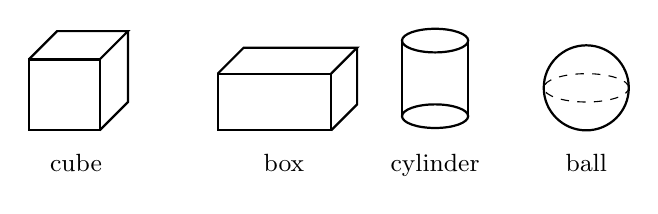
\begin{tikzpicture}[scale=0.6]
  \draw[thick] (0,0) rectangle (1.5,1.5);
  \draw[thick] (0,1.5) -- (0.6,2.1) -- (2.1,2.1) -- (1.5,1.5);
  \draw[thick] (2.1,2.1) -- (2.1,0.6) -- (1.5,0);
  \node[below, font=\small] at (1.0,-0.3) {cube};
  \begin{scope}[xshift=4.0cm]
  \draw[thick] (0,0) rectangle (2.4,1.2);
  \draw[thick] (0,1.2) -- (0.55,1.75) -- (2.95,1.75) -- (2.4,1.2);
  \draw[thick] (2.95,1.75) -- (2.95,0.55) -- (2.4,0);
  \node[below, font=\small] at (1.4,-0.3) {box};
  \end{scope}
  \begin{scope}[xshift=8.6cm]
  \draw[thick] (0,0.3) ellipse (0.7 and 0.25);
  \draw[thick] (-0.7,0.3) -- (-0.7,1.9);
  \draw[thick] (0.7,0.3) -- (0.7,1.9);
  \draw[thick] (0,1.9) ellipse (0.7 and 0.25);
  \node[below, font=\small] at (0,-0.3) {cylinder};
  \end{scope}
  \begin{scope}[xshift=11.8cm]
  \draw[thick] (0,0.9) circle (0.9);
  \draw[dashed] (0,0.9) ellipse (0.9 and 0.3);
  \node[below, font=\small] at (0,-0.3) {ball};
  \end{scope}
\end{tikzpicture}

{\small The first solids. Run a finger over a cube: you feel $6$ flat
faces and sharp edges; a ball has none.}
\end{omfigure}

\section{Exercises}

\begin{exercise}[$\star$]\label{exo:g2:shapes:1}
For each, count sides and corners and name it: a shape with $5$
sides; a shape with $3$ corners; a round shape.
\end{exercise}

\begin{exercise}[$\star$]\label{exo:g2:shapes:2}
Sort into ``polygon'' or ``not a polygon'': a square; a circle; a
triangle; a hexagon.
\end{exercise}

\begin{exercise}[$\star$]\label{exo:g2:shapes:3}
Make a right-angle tester by folding paper. Find three right angles
in the room, and one angle that is not right.
\end{exercise}

\begin{exercise}[$\star$]\label{exo:g2:shapes:4}
How many right angles has a square? A rectangle? A triangle can have
at most how many? (Try to draw one with two.)
\end{exercise}

\begin{exercise}[$\star$]\label{exo:g2:shapes:5}
On grid paper, copy a rectangle that is $4$ squares wide and $2$
tall, then a triangle with a $3$-square base.
\end{exercise}

\begin{exercise}[$\star$]\label{exo:g2:shapes:6}
Name the solid: a die; a can of soup; a football; a shoebox.
\end{exercise}

\begin{exercise}[$\star$]\label{exo:g2:shapes:7}
How many faces has a cube? What shape is each face? How many faces
has a box?
\end{exercise}

\begin{exercise}[$\star$]\label{exo:g2:shapes:8}
Which solids can roll: the cube, the box, the ball, the cylinder?
Why?
\end{exercise}

\begin{exercise}[$\star$]\label{exo:g2:shapes:9}
A shape has $6$ sides. What is it called? How many corners has it?
\end{exercise}

\begin{exercise}[$\star\star$]\label{exo:g2:shapes:10}
On grid paper, draw a house: a square for the wall
($4 \times 4$) with a triangle roof on top. How many sides and
corners has the whole outline of the house?
\end{exercise}

\chapter{Money and Measures}\label{ch:g2:measure}

Measuring rulers, kitchen scales, jugs, coins, clocks and
calendars: this chapter is about the numbers of everyday life ---
how long, how heavy, how much it holds, how much it costs, and what
time it is.

\section{Lengths, masses, capacities}

\begin{definition}[Everyday units]\label{def:g2:measure:units}
\begin{itemize}
  \item \emph{Length}: centimeter (cm) for small things, meter (m)
        for big ones, with $1$ m $= 100$ cm;
  \item \emph{mass}\index{mass}: gram (g) for light things, kilogram (kg) for
        heavy ones, with $1$ kg $= 1000$ g;
  \item \emph{capacity}\index{capacity} (how much a container holds): liter (L).
\end{itemize}
Smaller units and their exact rules come in \cref{ch:g3:measure}.
\end{definition}

\begin{example}[Which unit?]\label{ex:g2:measure:choose}
A crayon: about $9$ cm. A door: about $2$ m. An apple: about $150$
g. A big bag of flour: $1$ kg. A milk bottle: $1$ L. Guess the unit
before measuring --- it stops silly answers like ``the door is $2$
cm''.
\end{example}

\section{Money}

\begin{method}[Making an amount]\label{met:g2:measure:money}
With coins and bills of $1$, $2$, $5$, $10$, $20$:
\begin{enumerate}
  \item start with the biggest that fits, then fill the rest;
  \item to make $27$: a $20$, a $5$, and a $2$;
  \item there are often several ways --- $27$ is also $10 + 10 + 5 +
        2$.
\end{enumerate}
\end{method}

\begin{omfigure}
\begin{tikzpicture}[scale=0.9]
  \draw[thick, fill=omProp!20] (0,0) rectangle (1.3,0.7);
  \node[font=\small] at (0.65,0.35) {$20$};
  \node[font=\large] at (1.9,0.35) {$+$};
  \draw[thick, fill=omMeth!20] (2.85,0.35) circle (0.35);
  \node[font=\small] at (2.85,0.35) {$5$};
  \node[font=\large] at (3.8,0.35) {$+$};
  \draw[thick, fill=omDef!20] (4.7,0.35) circle (0.3);
  \node[font=\small] at (4.7,0.35) {$2$};
  \node[font=\large] at (5.6,0.35) {$=$};
  \node[font=\normalsize] at (6.5,0.35) {$27$};
\end{tikzpicture}

{\small Making $27$ with a bill and two coins --- and there are other
ways, like $10 + 10 + 5 + 2$.}
\end{omfigure}

\begin{example}[Change]\label{ex:g2:measure:change}
A book costs $14$; you pay with a $20$. The change is $20 - 14 =
6$, found by counting up: $14 \to 20$ is $6$
(\cref{met:g2:subtraction:countup}).
\end{example}

\section{Time}

\begin{method}[Half and quarter hours]\label{met:g2:measure:clock}
The long hand tells the minutes past the hour:
\begin{enumerate}
  \item straight up ($12$): on the hour --- $3{:}00$;
  \item quarter turn to the right ($3$): quarter past --- $3{:}15$;
  \item straight down ($6$): half past --- $3{:}30$;
  \item three-quarter turn ($9$): quarter to the next hour ---
        $3{:}45$, ``quarter to four''.
\end{enumerate}
\end{method}

\begin{omfigure}
\begin{tikzpicture}[scale=0.8]
  \foreach \x/\hh/\mm/\lbl in {0/3/3/{3:15}, 4/3/6/{3:30},
                                8/3/9/{3:45}} {
    \begin{scope}[xshift=\x cm]
    \draw[thick] (0,0) circle (1.2);
    \foreach \h in {1,...,12} {
      \node[font=\tiny] at ({90-\h*30}:0.98) {\h};
    }
    \draw[very thick, omDef] (0,0) -- ({90-(\hh+\mm/12)*30}:0.55);
    \draw[thick, omThm] (0,0) -- ({90-\mm*30}:0.95);
    \node[below, font=\small] at (0,-1.45) {\lbl};
    \end{scope}
  }
\end{tikzpicture}

{\small Quarter past, half past, quarter to: the long red hand at
the $3$, the $6$, the $9$.}
\end{omfigure}

\begin{example}[The calendar]\label{ex:g2:measure:calendar}
A year has $12$ months, in order: January, February, March, April,
May, June, July, August, September, October, November, December.
Most months have $30$ or $31$ days; February has $28$ (or $29$).
A date names the day and the month: ``the $5$th of March''.
\end{example}

\section{Exercises}

\begin{exercise}[$\star$]\label{exo:g2:measure:1}
Choose the unit (cm, m, g, kg or L): a pencil; the classroom
length; a feather; a schoolbag; a water bottle.
\end{exercise}

\begin{exercise}[$\star$]\label{exo:g2:measure:2}
Convert: $2$ m into cm; $300$ cm into m; $1$ kg into g.
\end{exercise}

\begin{exercise}[$\star$]\label{exo:g2:measure:3}
Make these amounts with coins and bills: $16$; \quad $23$; \quad
$35$. Give one way for each.
\end{exercise}

\begin{exercise}[$\star$]\label{exo:g2:measure:4}
Compute the change: pay $10$ for a $6$ toy; pay $20$ for a $17$
book; pay $50$ for a $32$ game.
\end{exercise}

\begin{exercise}[$\star$]\label{exo:g2:measure:5}
Read the time: long hand on $6$, short hand between $4$ and $5$;
long hand on $3$, short hand just after $8$.
\end{exercise}

\begin{exercise}[$\star$]\label{exo:g2:measure:6}
Draw a clock showing half past two. Where does each hand point?
\end{exercise}

\begin{exercise}[$\star$]\label{exo:g2:measure:7}
Name the month: after May; before January; the month of your
birthday.
\end{exercise}

\begin{exercise}[$\star$]\label{exo:g2:measure:8}
Lea buys a drink for $3$ and a cake for $4$. She pays with a $10$
bill. How much change?
\end{exercise}

\begin{exercise}[$\star$]\label{exo:g2:measure:9}
Which is heavier: a $1$ kg bag of sugar or $800$ g of apples? By how
many grams?
\end{exercise}

\begin{exercise}[$\star\star$]\label{exo:g2:measure:10}
Make $40$ with exactly four coins or bills (chosen from $1$, $2$,
$5$, $10$, $20$). Find two different ways.
\end{exercise}

\chapter{Solving Problems}\label{ch:g2:problems}

A story with numbers hides a question: add? take away? multiply?
This chapter gives a way to decide, uses simple bar pictures to
\emph{see} the operation, and reads information from tables and
pictograms.

\section{Choosing the operation}

\begin{method}[Which operation?]\label{met:g2:problems:choose}
\begin{enumerate}
  \item \emph{putting together, in all}: add ($+$);
  \item \emph{taking away, how many left, how many more}: subtract
        ($-$);
  \item \emph{so many equal groups}: multiply ($\times$);
  \item draw a quick picture when unsure, and always answer with a
        sentence.
\end{enumerate}
\end{method}

\begin{omfigure}
\begin{tikzpicture}[scale=0.6]
  % put together
  \draw[thick, fill=omDef!20] (0,0) rectangle (3,0.8);
  \draw[thick, fill=omThm!20] (3,0) rectangle (4.6,0.8);
  \node[font=\small] at (1.5,0.4) {$24$};
  \node[font=\small] at (3.8,0.4) {$15$};
  \draw[Stealth-Stealth] (0,-0.4) -- (4.6,-0.4);
  \node[below, font=\small] at (2.3,-0.5) {? in all: $24 + 15$};
  % compare
  \begin{scope}[xshift=8cm]
  \draw[thick, fill=omDef!20] (0,0.9) rectangle (4.6,1.7);
  \node[font=\small] at (2.3,1.3) {$40$};
  \draw[thick, fill=omThm!20] (0,0) rectangle (2.8,0.8);
  \node[font=\small] at (1.4,0.4) {$28$};
  \draw[Stealth-Stealth] (2.8,0.4) -- (4.6,0.4);
  \node[below, font=\small] at (2.3,-0.2) {? more: $40 - 28$};
  \end{scope}
\end{tikzpicture}

{\small Bar pictures: two bars joined mean an addition; two bars
compared mean a subtraction.}
\end{omfigure}

\begin{example}[A two-step problem]\label{ex:g2:problems:twostep}
``Sam buys $3$ packs of $6$ stickers, then gives $5$ away. How many
does he keep?''
\begin{enumerate}
  \item Groups: $3 \times 6 = 18$ stickers;
  \item give away: $18 - 5 = 13$.
\end{enumerate}
Sam keeps $13$ stickers. Reread the question: is the story really
finished? Here yes.
\end{example}

\begin{example}[A hidden extra number]\label{ex:g2:problems:extra}
``A $210$-page book\,\dots'' --- careful, not every number in a
story is needed. ``Ben has $8$ red and $6$ blue marbles and is $7$
years old. How many marbles?'' The age is a decoy: $8 + 6 = 14$
marbles. Sort the numbers before computing.
\end{example}

\section{Tables and pictograms}

\begin{example}[A table]\label{ex:g2:problems:table}
Cakes sold at a stall:
\begin{center}
\renewcommand{\arraystretch}{1.3}
\begin{tabular}{l|ccc}
 & Saturday & Sunday & total \\
\hline
muffins & $12$ & $9$ & $21$ \\
tarts & $7$ & $10$ & $17$ \\
\end{tabular}
\end{center}
Reading: Sunday tarts, $10$. Computing: muffins over the two days,
$12 + 9 = 21$; more tarts on Sunday than Saturday by $10 - 7 = 3$.
\end{example}

\begin{example}[A pictogram]\label{ex:g2:problems:pictogram}
Read the key first: here one apple stands for $2$ pieces of fruit.

\begin{omfigure}
\begin{tikzpicture}[scale=0.62]
  \node[left, font=\small] at (0,2) {red};
  \foreach \i in {0,1,2,3} \fill[omThm] (0.5+\i*0.75,2) circle (0.24);
  \node[left, font=\small] at (0,1) {green};
  \foreach \i in {0,1} \fill[omMeth] (0.5+\i*0.75,1) circle (0.24);
  \node[left, font=\small] at (0,0) {yellow};
  \foreach \i in {0,1,2} \fill[omProp] (0.5+\i*0.75,0) circle (0.24);
  \node[right, font=\small] at (4.0,1) {key: one dot $= 2$ fruits};
\end{tikzpicture}

{\small A pictogram: red shows $4$ dots, so $4 \times 2 = 8$ red
fruits; green $2$ dots, $4$ fruits; yellow $3$ dots, $6$ fruits.}
\end{omfigure}
\end{example}

\section{Exercises}

\begin{exercise}[$\star$]\label{exo:g2:problems:1}
Name the operation (do not compute): ``$34$ and $28$ marbles put
together''; ``$50$ sweets, $12$ eaten''; ``$4$ boxes of $5$
apples''; ``Ana has $30$, Leo has $18$: how many more has Ana?''.
\end{exercise}

\begin{exercise}[$\star$]\label{exo:g2:problems:2}
Solve: ``A car park has $156$ cars; $48$ leave. How many stay?''
\end{exercise}

\begin{exercise}[$\star$]\label{exo:g2:problems:3}
Solve: ``$5$ children each pick $4$ flowers. How many flowers in
all?''
\end{exercise}

\begin{exercise}[$\star$]\label{exo:g2:problems:4}
Draw a bar picture, then solve: ``Tom has $45$ cards, Mia has $17$
fewer. How many has Mia?''
\end{exercise}

\begin{exercise}[$\star$]\label{exo:g2:problems:5}
Two steps: ``A crate holds $6$ bottles. A shop gets $4$ crates and
sells $9$ bottles. How many bottles remain?''
\end{exercise}

\begin{exercise}[$\star$]\label{exo:g2:problems:6}
Find and cross out the useless number, then solve: ``Ben is $8$
years old and has $23$ marbles. He wins $15$ more. How many marbles
now?''
\end{exercise}

\begin{exercise}[$\star$]\label{exo:g2:problems:7}
Using the table of \cref{ex:g2:problems:table}: how many tarts sold
over the two days? How many cakes of all kinds on Saturday?
\end{exercise}

\begin{exercise}[$\star$]\label{exo:g2:problems:8}
Using the pictogram of \cref{ex:g2:problems:pictogram}: how many
fruits in all? Which colour has the most?
\end{exercise}

\begin{exercise}[$\star$]\label{exo:g2:problems:9}
Solve: ``A ribbon is $80$ cm long. Lea cuts off $35$ cm. How long is
the piece that remains?''
\end{exercise}

\begin{exercise}[$\star\star$]\label{exo:g2:problems:10}
``A baker makes $5$ trays of $4$ cakes in the morning and $3$ trays
of $4$ cakes in the afternoon. How many cakes that day?'' (Two
multiplications, then a \omterm{def:g1:addition:def}{sum} --- or count the trays first!)
\end{exercise}


% ============================================================================
% Grade 3 (age 8–9) — third year of primary school.
%
% One chapter per file. Solutions live in solutions/, one file per chapter,
% same numbering.
% ============================================================================
\part{Grade 3 (Age 8--9)}

\chapter{Numbers up to 10\,000}\label{ch:g3:numbers}

One thousand, two thousand, three thousand\,\dots\ big numbers are
built from small ones, using a wonderful idea: the \emph{place} of a
digit tells its value. This chapter teaches how to read, write,
compare and order numbers up to $10\,000$.

\section{Reading and writing numbers}

\begin{definition}[Place value]\label{def:g3:numbers:place}
A number is written with the digits $0, 1, 2, \dots, 9$. Reading from
the right, the places are: units, tens, hundreds, thousands. In
$3\,254$:
\[
3\,254 = 3 \text{ thousands} + 2 \text{ hundreds} + 5 \text{ tens}
+ 4 \text{ units}.
\]
\end{definition}

\begin{omfigure}
\begin{tikzpicture}[scale=0.9]
  \draw (0,0) grid[xstep=1.7, ystep=0.8] (6.8,1.6);
  \node[font=\small] at (0.85,1.2) {thousands};
  \node[font=\small] at (2.55,1.2) {hundreds};
  \node[font=\small] at (4.25,1.2) {tens};
  \node[font=\small] at (5.95,1.2) {units};
  \node[font=\large, omDef] at (0.85,0.4) {$3$};
  \node[font=\large, omDef] at (2.55,0.4) {$2$};
  \node[font=\large, omDef] at (4.25,0.4) {$5$};
  \node[font=\large, omDef] at (5.95,0.4) {$4$};
\end{tikzpicture}

{\small The place-value table of $3\,254$, read ``three thousand two
hundred fifty-four''.}
\end{omfigure}

\begin{example}[The zero that holds a place]\label{ex:g3:numbers:zero}
``Four thousand and seven'' is written $4\,007$: a $4$ in the
thousands, a $7$ in the units, and \emph{zeros} in between to keep
each digit in its right place. Without them, $47$ would be a very
different number!
\end{example}

\begin{example}[Exchanging]\label{ex:g3:numbers:exchange}
Ten units make one ten; ten tens make one hundred; ten hundreds make
one thousand. So $10$ hundreds $= 1\,000$, and $32$ tens
$= 320$: the number $320$ contains $32$ tens (not just the digit
$2$!).
\end{example}

\section{Comparing and ordering}

\begin{method}[Comparing two numbers]\label{met:g3:numbers:compare}
\begin{enumerate}
  \item Count the digits: more digits means a bigger number
        ($1\,002 > 998$).
  \item Same number of digits: compare digit by digit starting from
        the \emph{left}. The first difference decides:
        $5\,614 > 5\,589$ because $6 > 5$ at the hundreds.
  \item Write the answer with the signs $<$ (smaller than) or $>$
        (bigger than): the open side always faces the bigger number.
\end{enumerate}
\end{method}

\begin{omfigure}
\begin{tikzpicture}[scale=1.1]
  \draw[-Stealth] (-0.3,0) -- (10.5,0);
  \foreach \i in {0,1,...,10} \draw (\i,-0.08) -- (\i,0.08);
  \node[below, font=\small] at (0,-0.1) {$0$};
  \node[below, font=\small] at (5,-0.1) {$500$};
  \node[below, font=\small] at (10,-0.1) {$1000$};
  \fill[omThm] (2.4,0) circle (2pt) node[above, font=\small] {$240$};
  \fill[omDef] (6.9,0) circle (2pt) node[above, font=\small] {$690$};
  \fill[omMeth] (9.05,0) circle (2pt) node[above, font=\small] {$905$};
\end{tikzpicture}

{\small Numbers on a line graduated in hundreds: further right means
bigger. $240 < 690 < 905$.}
\end{omfigure}

\begin{example}\label{ex:g3:numbers:order}
Order from smallest to biggest: $780$, $8\,700$, $807$, $87$.
First by the number of digits: $87$ (two), then $780$ and $807$
(three), then $8\,700$ (four). Between $780$ and $807$: compare the
hundreds digits, $7 < 8$, so $780 < 807$. Final order:
\[
87 < 780 < 807 < 8\,700 .
\]
\end{example}

\section{Even and odd}

\begin{definition}[Even, odd]\label{def:g3:numbers:evenodd}
A number is \emph{even}\index{even number} when it can be split into
two equal whole parts --- its units digit is $0$, $2$, $4$, $6$ or
$8$. Otherwise it is \emph{odd}\index{odd number} (units digit $1$,
$3$, $5$, $7$ or $9$).
\end{definition}

\begin{example}
$46$ is even ($46 = 23 + 23$); $47$ is odd (two equal parts would
need half an object). Only the \emph{last} digit matters: $3\,578$ is
even, $2\,341$ is odd.
\end{example}

\begin{omfigure}
\begin{tikzpicture}[scale=0.45]
  \foreach \i in {0,...,5} \fill[omDef] ({\i},0) circle (0.28);
  \foreach \i in {0,...,5} \fill[omDef] ({\i},1) circle (0.28);
  \node[below, font=\small] at (2.5,-0.7) {$12$: even, two equal rows};
  \begin{scope}[xshift=10.5cm]
  \foreach \i in {0,...,5} \fill[omThm] ({\i},0) circle (0.28);
  \foreach \i in {0,...,4} \fill[omThm] ({\i},1) circle (0.28);
  \node[below, font=\small] at (2.5,-0.7) {$11$: odd, one dot alone};
  \end{scope}
\end{tikzpicture}

{\small Even numbers split into two equal rows; odd numbers always
leave one alone.}
\end{omfigure}

\section{Exercises}

\begin{exercise}[$\star$]\label{exo:g3:numbers:1}
Write in digits: ``two thousand three hundred forty-five''; ``six
thousand and fifty''; ``nine thousand and one''.
\end{exercise}

\begin{exercise}[$\star$]\label{exo:g3:numbers:2}
Write in words: $1\,208$; \quad $4\,070$; \quad $9\,999$.
\end{exercise}

\begin{exercise}[$\star$]\label{exo:g3:numbers:3}
In $7\,382$: which digit is in the tens place? In the thousands
place? How many \emph{hundreds} does the number contain in total
(careful: not just the hundreds digit --- think of
\cref{ex:g3:numbers:exchange})?
\end{exercise}

\begin{exercise}[$\star$]\label{exo:g3:numbers:4}
Decompose as in \cref{def:g3:numbers:place}:
$5\,631$; \quad $2\,046$; \quad $8\,500$.
\end{exercise}

\begin{exercise}[$\star$]\label{exo:g3:numbers:5}
Copy and complete with $<$ or $>$:
\[
456 \;?\; 465, \qquad
1\,203 \;?\; 989, \qquad
6\,090 \;?\; 6\,009, \qquad
9\,999 \;?\; 10\,000 .
\]
\end{exercise}

\begin{exercise}[$\star$]\label{exo:g3:numbers:6}
Order from smallest to biggest: $530$; \ $3\,500$; \ $353$; \ $5\,033$;
\ $503$.
\end{exercise}

\begin{exercise}[$\star$]\label{exo:g3:numbers:7}
On a number line graduated in hundreds from $0$ to $1\,000$, place
(approximately) the numbers $150$, $480$, $820$ and $990$.
\end{exercise}

\begin{exercise}[$\star$]\label{exo:g3:numbers:8}
Even or odd? \ $34$; \ $57$; \ $70$; \ $2\,481$; \ $6\,548$.
\end{exercise}

\begin{exercise}[$\star$]\label{exo:g3:numbers:9}
Count by steps: from $2\,970$, count five steps of $10$; from $860$,
count four steps of $100$; from $9\,996$, count four steps of $1$.
What do you notice at the end of the last one?
\end{exercise}

\begin{exercise}[$\star\star$]\label{exo:g3:numbers:10}
Using each of the digits $3$, $7$, $0$, $5$ exactly once, write the
biggest possible four-digit number, then the smallest one (a number
cannot start with $0$).
\end{exercise}

\begin{exercise}[$\star\star$]\label{exo:g3:numbers:11}
I am a three-digit number. My digits are $2$, $5$ and $8$, I am even,
and I am bigger than $800$. Who am I?
\end{exercise}

\chapter{Addition and Subtraction}\label{ch:g3:addsub}

Adding means putting together; subtracting means taking away, or
finding what is missing. This chapter trains the two column methods
--- with their famous carries and borrows --- and the mental tricks
that often make columns unnecessary.

\section{Column addition}

\begin{method}[Adding in columns]\label{met:g3:addsub:add}
\begin{enumerate}
  \item Write the numbers one under the other, units under units,
        tens under tens (line up on the \emph{right});
  \item add the units; if the \omterm{def:g1:addition:def}{sum} passes $9$, write its units digit
        and \emph{carry} the ten to the next column (a small $1$);
  \item continue with the tens, the hundreds, \dots, adding the carry
        each time.
\end{enumerate}
\end{method}

\begin{example}\label{ex:g3:addsub:add}
Compute $457 + 368$:
\[
\begin{array}{r}
{\scriptstyle 1}\ \ {\scriptstyle 1}\ \ \phantom{0} \\[-3pt]
4\,5\,7 \\
+\ 3\,6\,8 \\
\hline
8\,2\,5
\end{array}
\]
Units: $7 + 8 = 15$: write $5$, carry $1$. Tens:
$5 + 6 + 1 = 12$: write $2$, carry $1$. Hundreds: $4 + 3 + 1 = 8$.
Result: $825$.
\end{example}

\begin{example}[Mental addition]\label{ex:g3:addsub:mental}
Look for friendly numbers before reaching for columns:
\begin{itemize}
  \item \emph{make a ten}: $47 + 8 = 47 + 3 + 5 = 50 + 5 = 55$;
  \item \emph{jump by parts}: $256 + 130 = 256 + 100 + 30 = 386$;
  \item \emph{reorder}: $17 + 59 + 3 = (17 + 3) + 59 = 79$.
\end{itemize}
\end{example}

\begin{omfigure}
\begin{tikzpicture}[scale=1.05]
  \draw[-Stealth] (-0.2,0) -- (10.4,0);
  \foreach \x/\l in {0.56/{256}, 5.56/{356}, 7.06/{386}}
    { \draw (\x,-0.08) -- (\x,0.08);
      \node[below, font=\small] at (\x,-0.1) {$\l$}; }
  \draw[-Stealth, omDef, thick] (0.56,0.25) .. controls (2.8,1.15) ..
    (5.56,0.25);
  \node[omDef, font=\small] at (3.05,1.05) {$+100$};
  \draw[-Stealth, omThm, thick] (5.56,0.25) .. controls (6.3,0.8) ..
    (7.06,0.25);
  \node[omThm, font=\small] at (6.3,0.85) {$+30$};
\end{tikzpicture}

{\small Mental addition as jumps on the number line: $256 + 130$ in
two hops, first the hundreds, then the tens.}
\end{omfigure}

\section{Column subtraction}

\begin{method}[Subtracting in columns]\label{met:g3:addsub:sub}
\begin{enumerate}
  \item Write the bigger number on top, aligned on the right;
  \item subtract column by column, starting from the units;
  \item if the top digit is too small, \emph{borrow}: take one from
        the next place on the top row (it is worth ten in the current
        column);
  \item \emph{check}: the result plus the subtracted number must give
        back the top number.
\end{enumerate}
\end{method}

\begin{example}\label{ex:g3:addsub:sub}
Compute $603 - 147$:
\[
\begin{array}{r}
6\,0\,3 \\
-\ 1\,4\,7 \\
\hline
4\,5\,6
\end{array}
\]
Units: $3 - 7$ impossible; borrow through: $603$ becomes
$5$ hundreds, $9$ tens, $13$ units. Then $13 - 7 = 6$;
tens $9 - 4 = 5$; hundreds $5 - 1 = 4$. Result: $456$.
Check: $456 + 147 = 603$.
\end{example}

\begin{omfigure}
\begin{tikzpicture}[scale=0.82]
  % before: 6 hundreds, 0 tens, 3 units
  \node[font=\small] at (2.5,2.25) {$603$ before the borrow};
  \foreach \i in {0,...,5}
    \draw[omProp, fill=omProp!25] (0.62*\i,0.7) rectangle
      (0.62*\i+0.44,1.7);
  \node[below, font=\footnotesize] at (1.7,0.55) {$6$ hundreds};
  \node[font=\footnotesize] at (4.35,1.2) {$0$ tens};
  \foreach \i in {0,1,2} \fill[omDef] (5.4+0.4*\i,1.2) circle (0.13);
  \node[below, font=\footnotesize] at (5.8,0.55) {$3$ units};
  % after: 5 hundreds, 9 tens, 13 units
  \begin{scope}[yshift=-3.3cm]
  \node[font=\small] at (2.5,2.25) {$603$ after the borrow};
  \foreach \i in {0,...,4}
    \draw[omProp, fill=omProp!25] (0.62*\i,0.7) rectangle
      (0.62*\i+0.44,1.7);
  \node[below, font=\footnotesize] at (1.4,0.55) {$5$ hundreds};
  \foreach \i in {0,...,8}
    \draw[omThm, very thick] (3.5+0.22*\i,0.7) -- (3.5+0.22*\i,1.7);
  \node[below, font=\footnotesize] at (4.4,0.55) {$9$ tens};
  \foreach \i in {0,...,6} \fill[omDef] (6.1+0.4*\i,1.45) circle (0.13);
  \foreach \i in {0,...,5} \fill[omDef] (6.1+0.4*\i,0.95) circle (0.13);
  \node[below, font=\footnotesize] at (7.3,0.55) {$13$ units};
  \end{scope}
\end{tikzpicture}

{\small The borrow of $603 - 147$ in pictures: one hundred is untied
into ten tens, and one of those tens into ten units. Same amount,
new clothes --- $6\,\vert\,0\,\vert\,3$ becomes
$5\,\vert\,9\,\vert\,13$, and every column can now subtract.}
\end{omfigure}

\begin{example}[Subtraction as a missing part]\label{ex:g3:addsub:missing}
``Lila has $35$ marbles, Tom has $52$: how many more has Tom?'' is
the subtraction $52 - 35$. Mentally, count \emph{up} from $35$:
$35 \to 40$ is $5$, then $40 \to 52$ is $12$; in total
$5 + 12 = 17$. Counting up is often easier than borrowing.
\end{example}

\begin{omfigure}
\begin{tikzpicture}[scale=1.05]
  \draw[-Stealth] (-0.2,0) -- (10.4,0);
  \foreach \x/\l in {1.0/{35}, 3.5/{40}, 9.5/{52}}
    { \draw (\x,-0.08) -- (\x,0.08);
      \node[below, font=\small] at (\x,-0.1) {$\l$}; }
  \draw[-Stealth, omDef, thick] (1.0,0.25) .. controls (2.2,0.9) ..
    (3.5,0.25);
  \node[omDef, font=\small] at (2.25,0.92) {$+5$};
  \draw[-Stealth, omThm, thick] (3.5,0.25) .. controls (6.5,1.2) ..
    (9.5,0.25);
  \node[omThm, font=\small] at (6.5,1.1) {$+12$};
\end{tikzpicture}

{\small Computing $52 - 35$ by counting up: first to the friendly
$40$, then to $52$. The answer is the total of the hops:
$5 + 12 = 17$.}
\end{omfigure}

\section{Orders of magnitude}

\begin{method}[Estimating before computing]\label{met:g3:addsub:estimate}
Before any column computation, round the numbers to friendly ones and
compute an \emph{estimate}. After computing, compare: a result far
from the estimate signals a mistake.
\end{method}

\begin{example}
For $487 + 312$: the estimate is $500 + 300 = 800$. The column
result, $799$, is close: plausible. If you had found $1\,099$
(a missed alignment), the estimate would have warned you.
\end{example}

\section{Exercises}

\begin{exercise}[$\star$]\label{exo:g3:addsub:1}
Compute in columns: $346 + 253$; \quad $478 + 265$; \quad
$1\,536 + 2\,876$.
\end{exercise}

\begin{exercise}[$\star$]\label{exo:g3:addsub:2}
Compute in columns, then check by an addition: $587 - 234$; \quad
$805 - 348$; \quad $1\,000 - 463$.
\end{exercise}

\begin{exercise}[$\star$]\label{exo:g3:addsub:3}
Compute mentally by making tens: $38 + 7$; \quad $56 + 9$; \quad
$45 + 28$ (add $30$, take away $2$).
\end{exercise}

\begin{exercise}[$\star$]\label{exo:g3:addsub:4}
Compute mentally by jumps: $340 + 220$; \quad $675 + 210$; \quad
$512 - 300$; \quad $840 - 220$.
\end{exercise}

\begin{exercise}[$\star$]\label{exo:g3:addsub:5}
Compute $63 - 47$ by counting up (as in
\cref{ex:g3:addsub:missing}), then check in columns.
\end{exercise}

\begin{exercise}[$\star$]\label{exo:g3:addsub:6}
Estimate first (round to hundreds), then compute exactly:
$492 + 218$; \quad $913 - 388$.
\end{exercise}

\begin{exercise}[$\star$]\label{exo:g3:addsub:7}
A school has $348$ girls and $296$ boys. How many students in all?
Write the operation, compute, and answer with a sentence.
\end{exercise}

\begin{exercise}[$\star$]\label{exo:g3:addsub:8}
A book has $224$ pages; Nora has read $178$. How many pages are left
to read?
\end{exercise}

\begin{exercise}[$\star$]\label{exo:g3:addsub:9}
Complete the holes (work column by column):
\[
\begin{array}{r}
3\,?\,7 \\
+\ ?\,2\,? \\
\hline
8\,6\,2
\end{array}
\]
Is there only one way to fill the three holes? Explain.
\end{exercise}

\begin{exercise}[$\star\star$]\label{exo:g3:addsub:10}
A bakery sold $145$ croissants in the morning and $89$ in the
afternoon; $17$ croissants were left unsold at closing time. How many
croissants were baked that day? (Two steps.)
\end{exercise}

\begin{exercise}[$\star\star$]\label{exo:g3:addsub:11}
Theo says: ``to compute $500 - 199$, I compute $500 - 200$ and then
add $1$.'' Is he right? Compute both ways, and explain his trick.
\end{exercise}

\chapter{Multiplication}\label{ch:g3:mult}

Three bags of seven marbles: you could add $7 + 7 + 7$, but there is
a faster way --- multiplication, the operation of repeated addition.
This chapter builds the multiplication tables from pictures, then
teaches the column method.

\section{What multiplying means}

\begin{definition}[Multiplication]\label{def:g3:mult:def}
The product $3 \times 7$ means ``three times seven'':
\[
3 \times 7 = 7 + 7 + 7 = 21 .
\]
On a picture, $3 \times 7$ is a rectangle of dots: $3$ rows of $7$
dots.
\end{definition}

\begin{omfigure}
\begin{tikzpicture}[scale=0.42]
  \foreach \r in {0,1,2}
    \foreach \c in {0,...,6}
      \fill[omDef] (\c,-\r) circle (0.27);
  \node[right, font=\small] at (7.0,-1.0) {$3$ rows of $7$:\ \
  $3 \times 7 = 21$};
  \begin{scope}[yshift=-4.4cm]
  \foreach \r in {0,...,6}
    \foreach \c in {0,1,2}
      \fill[omThm] (\c,-\r*0.62) circle (0.27);
  \node[right, font=\small] at (7.0,-1.9) {$7$ rows of $3$:\ \
  $7 \times 3 = 21$ too!};
  \end{scope}
\end{tikzpicture}

{\small The same $21$ dots, counted by rows or by columns: the order
of a product does not matter. Knowing $3 \times 7$ gives
$7 \times 3$ for free --- half the tables to learn!}
\end{omfigure}

\begin{proposition}[Rules that help]\label{prop:g3:mult:rules}
\begin{enumerate}
  \item The order does not matter: $a \times b = b \times a$.
  \item Multiplying by $1$ changes nothing; multiplying by $0$ gives
        $0$.
  \item Multiplying by $10$ appends a zero: $34 \times 10 = 340$;
        by $100$, two zeros.
  \item A table can be rebuilt from its neighbors:
        $6 \times 8 = 5 \times 8 + 8 = 40 + 8 = 48$.
\end{enumerate}
\end{proposition}
\admitted

\begin{example}[The table square]\label{ex:g3:mult:table}
All the tables fit in one square. To read $6 \times 7$: row $6$,
column $7$.
\begin{center}
\renewcommand{\arraystretch}{1.15}
\begin{tabular}{c|ccccccccc}
$\times$ & $1$ & $2$ & $3$ & $4$ & $5$ & $6$ & $7$ & $8$ & $9$ \\
\hline
$1$ & 1 & 2 & 3 & 4 & 5 & 6 & 7 & 8 & 9 \\
$2$ & 2 & 4 & 6 & 8 & 10 & 12 & 14 & 16 & 18 \\
$3$ & 3 & 6 & 9 & 12 & 15 & 18 & 21 & 24 & 27 \\
$4$ & 4 & 8 & 12 & 16 & 20 & 24 & 28 & 32 & 36 \\
$5$ & 5 & 10 & 15 & 20 & 25 & 30 & 35 & 40 & 45 \\
$6$ & 6 & 12 & 18 & 24 & 30 & 36 & 42 & 48 & 54 \\
$7$ & 7 & 14 & 21 & 28 & 35 & 42 & 49 & 56 & 63 \\
$8$ & 8 & 16 & 24 & 32 & 40 & 48 & 56 & 64 & 72 \\
$9$ & 9 & 18 & 27 & 36 & 45 & 54 & 63 & 72 & 81 \\
\end{tabular}
\end{center}
The square is symmetric across its diagonal --- that is rule 1 made
visible.
\end{example}

\section{Column multiplication}

\begin{method}[Multiplying by a one-digit number]\label{met:g3:mult:column}
To compute $234 \times 6$:
\begin{enumerate}
  \item multiply the units: $4 \times 6 = 24$: write $4$, carry $2$;
  \item multiply the tens and add the carry:
        $3 \times 6 + 2 = 20$: write $0$, carry $2$;
  \item multiply the hundreds and add the carry:
        $2 \times 6 + 2 = 14$: write $14$.
\end{enumerate}
\[
\begin{array}{r}
2\,3\,4 \\
\times \quad 6 \\
\hline
1\,4\,0\,4
\end{array}
\]
Estimate to check: $234$ is close to $200$, and
$200 \times 6 = 1\,200$: the answer $1\,404$ is plausible.
\end{method}

\begin{example}[Splitting to multiply mentally]\label{ex:g3:mult:split}
The column method secretly splits the number by places. Mentally, do
the same:
\[
23 \times 4 = (20 + 3) \times 4 = 20 \times 4 + 3 \times 4
= 80 + 12 = 92 .
\]
And with a friendly neighbor: $99 \times 5 = 100 \times 5 - 5 =
495$.
\end{example}

\begin{omfigure}
\begin{tikzpicture}[scale=0.55]
  \fill[omDef!18] (0,0) rectangle (10,4);
  \fill[omThm!18] (10,0) rectangle (11.5,4);
  \draw[thick] (0,0) rectangle (11.5,4);
  \draw[thick] (10,0) -- (10,4);
  \node[font=\small] at (5,2) {$20 \times 4 = 80$};
  \node[font=\small, rotate=90] at (10.75,2) {$3 {\times} 4$};
  \node[below, font=\small] at (5,0) {$20$};
  \node[below, font=\small] at (10.75,0) {$3$};
  \node[left, font=\small] at (0,2) {$4$};
\end{tikzpicture}

{\small Why splitting works: a $23 \times 4$ rectangle of unit
squares is a $20 \times 4$ part plus a $3 \times 4$ part ---
$80 + 12 = 92$ squares.}
\end{omfigure}

\section{Multiplication in problems}

\begin{example}\label{ex:g3:mult:problem}
A minibus carries $9$ passengers. How many passengers can $27$
minibuses carry?
\begin{enumerate}
  \item It is a multiplication: $27$ groups of $9$.
  \item $27 \times 9 = 243$ (columns, or
        $27 \times 9 = 27 \times 10 - 27 = 270 - 27$).
  \item Sentence: the minibuses can carry $243$ passengers.
\end{enumerate}
\end{example}

\section{Exercises}

\begin{exercise}[$\star$]\label{exo:g3:mult:1}
Write as a multiplication, then compute:
$8 + 8 + 8 + 8$; \quad $5 + 5 + 5$; \quad
$20 + 20 + 20 + 20 + 20$.
\end{exercise}

\begin{exercise}[$\star$]\label{exo:g3:mult:2}
Recite and complete: $6 \times 7$; \ $8 \times 4$; \ $9 \times 9$;
\ $7 \times 8$; \ $6 \times 6$.
\end{exercise}

\begin{exercise}[$\star$]\label{exo:g3:mult:3}
Draw a dot rectangle for $4 \times 6$, then one for $6 \times 4$.
What do you notice about the two counts?
\end{exercise}

\begin{exercise}[$\star$]\label{exo:g3:mult:4}
Compute using the rules of \cref{prop:g3:mult:rules}:
$56 \times 10$; \quad $8 \times 100$; \quad $73 \times 0$; \quad
$45 \times 1$; \quad $30 \times 10$.
\end{exercise}

\begin{exercise}[$\star$]\label{exo:g3:mult:5}
Compute in columns: $132 \times 3$; \quad $217 \times 4$; \quad
$408 \times 7$.
\end{exercise}

\begin{exercise}[$\star$]\label{exo:g3:mult:6}
Compute mentally by splitting (as in \cref{ex:g3:mult:split}):
$31 \times 5$; \quad $42 \times 3$; \quad $25 \times 6$.
\end{exercise}

\begin{exercise}[$\star$]\label{exo:g3:mult:7}
Compute with a friendly neighbor: $99 \times 7$; \quad
$101 \times 6$; \quad $98 \times 5$.
\end{exercise}

\begin{exercise}[$\star$]\label{exo:g3:mult:8}
Estimate first, then compute: $389 \times 5$ (estimate with $400$);
$612 \times 8$ (estimate with $600$).
\end{exercise}

\begin{exercise}[$\star$]\label{exo:g3:mult:9}
An egg box holds $6$ eggs. How many eggs are in $38$ boxes? Write
the operation, compute, answer with a sentence.
\end{exercise}

\begin{exercise}[$\star\star$]\label{exo:g3:mult:10}
A classroom has $8$ rows of $4$ desks; each desk seats $2$ students.
How many students can the room seat? (Two multiplications.)
\end{exercise}

\begin{exercise}[$\star\star$]\label{exo:g3:mult:11}
Find all the ways of arranging $24$ chairs into equal rows (rows of
$1$, of $2$, \dots). Which arrangements are possible? (Use the table
square: look for $24$ inside it.)
\end{exercise}

\begin{exercise}[$\star\star$]\label{exo:g3:mult:12}
Zoe computes $47 \times 6$ like this: $40 \times 6 = 240$,
$7 \times 6 = 42$, and then $240 + 42 = 282$. Léa computes
$47 \times 6 = 50 \times 6 - 3 \times 6 = 300 - 18 = 282$. Explain
each method. Which do you prefer for $38 \times 4$? Compute it both
ways.
\end{exercise}

\chapter{Sharing and Division}\label{ch:g3:division}

Twenty marbles shared fairly among four children: how many each?
Division answers all the sharing questions --- and the grouping
questions too --- and it is multiplication's twin: one undoes the
other.

\section{Two faces of division}

\begin{definition}[Division]\label{def:g3:division:def}
The division $20 \div 4$ answers two kinds of questions:
\begin{itemize}
  \item \emph{sharing}: $20$ marbles shared among $4$ children ---
        how many marbles \emph{each}? ($5$ each);
  \item \emph{grouping}: $20$ marbles put in bags of $4$ --- how many
        \emph{bags}? ($5$ bags).
\end{itemize}
Both questions have the same answer, because both undo the same
multiplication: $4 \times 5 = 20$.
\end{definition}

\begin{omfigure}
\begin{tikzpicture}[scale=0.42]
  \foreach \g in {0,1,2,3} {
    \draw[omExo, rounded corners] (\g*5-0.6,-0.65) rectangle
      (\g*5+3.4,0.65);
    \foreach \c in {0,...,4} \fill[omDef] (\g*5+\c*0.7,0) circle (0.25);
  }
  \node[below, font=\small] at (9,-1.2)
    {$20$ marbles, $4$ equal groups: $5$ in each group};
\end{tikzpicture}

{\small Sharing $20$ into $4$ equal groups. Grouping by $4$ instead
would give $5$ groups --- the same division.}
\end{omfigure}

\begin{method}[Dividing with the tables]\label{met:g3:division:tables}
To compute $42 \div 6$, ask: ``$6$ times \emph{what} makes $42$?''
The table of $6$ answers: $6 \times 7 = 42$, so $42 \div 6 = 7$.
Every division question is a multiplication question read
backwards.
\end{method}

\section{When it does not come out even}

\begin{definition}[Remainder]\label{def:g3:division:remainder}
Sharing $23$ marbles among $4$ children gives $5$ marbles each ---
and $3$ marbles \emph{left over}, not enough for another round. We
write
\[
23 = 4 \times 5 + 3 ,
\]
and say: the \emph{quotient} is $5$, the
\emph{remainder}\index{remainder} is $3$. The remainder is always
smaller than the number of children --- otherwise another round of
sharing would be possible.
\end{definition}

\begin{omfigure}
\begin{tikzpicture}[scale=0.42]
  \foreach \g in {0,1,2,3} {
    \draw[omExo, rounded corners] (\g*5-0.6,-0.65) rectangle
      (\g*5+3.4,0.65);
    \foreach \c in {0,...,4} \fill[omDef] (\g*5+\c*0.7,0) circle (0.25);
  }
  \foreach \c in {0,1,2} \fill[omThm] (20.4+\c*0.7,0) circle (0.25);
  \node[below, font=\small] at (10.4,-1.2)
    {$23 = 4 \times 5 + 3$: quotient $5$, remainder $3$ (in red)};
\end{tikzpicture}

{\small Sharing $23$ among $4$: after $5$ rounds, $3$ marbles remain
--- too few for a $6$th round.}
\end{omfigure}

\begin{example}\label{ex:g3:division:remainder}
Divide $58$ by $7$. Scan the table of $7$:
$7 \times 8 = 56$ is the biggest product that fits under $58$
($7 \times 9 = 63$ is too much). So
\[
58 = 7 \times 8 + 2 :
\]
quotient $8$, remainder $2$. Check: $56 + 2 = 58$, and $2 < 7$.
\end{example}

\begin{method}[Interpreting the remainder]\label{met:g3:division:interpret}
After dividing, return to the story:
\begin{enumerate}
  \item ``how many each / how many full groups?'' --- the quotient;
  \item ``how many left over?'' --- the remainder;
  \item ``how many boxes to hold everything?'' --- the quotient
        \emph{plus one} if the remainder is not zero.
\end{enumerate}
\end{method}

\begin{example}\label{ex:g3:division:interpret}
$58$ students go canoeing, $7$ per canoe. $58 = 7 \times 8 + 2$:
eight canoes are full, and $2$ students remain --- they need a canoe
too. So $9$ canoes must be booked.
\end{example}

\section{Halves, thirds, quarters}

\begin{definition}[Half, third, quarter]\label{def:g3:division:half}
The \emph{half} of a number is the result of dividing it by $2$; the
\emph{third}, by $3$; the \emph{quarter}, by $4$. For instance the
half of $18$ is $9$, the third of $18$ is $6$, the quarter of $36$
is $9$.
\end{definition}

\begin{example}[Doubles and halves go together]\label{ex:g3:division:double}
The half of $46$: since $46 = 40 + 6$, half of each part gives
$20 + 3 = 23$. Check with the double: $23 + 23 = 46$. Knowing
doubles by heart ($25 \to 50$, $45 \to 90$, $150 \to 300$) makes
halves instantaneous.
\end{example}

\section{Exercises}

\begin{exercise}[$\star$]\label{exo:g3:division:1}
Compute using the tables backwards: $36 \div 4$; \quad $63 \div 9$;
\quad $40 \div 5$; \quad $56 \div 8$.
\end{exercise}

\begin{exercise}[$\star$]\label{exo:g3:division:2}
For each division, write the equality $a = b \times q + r$ and give
the quotient and the remainder: $17 \div 5$; \quad $30 \div 4$; \quad
$50 \div 6$.
\end{exercise}

\begin{exercise}[$\star$]\label{exo:g3:division:3}
$28$ marbles are shared among $6$ children. How many marbles each,
and how many left over? Draw the sharing if it helps.
\end{exercise}

\begin{exercise}[$\star$]\label{exo:g3:division:4}
Compute: the half of $68$; the third of $27$; the quarter of $48$;
the half of $150$.
\end{exercise}

\begin{exercise}[$\star$]\label{exo:g3:division:5}
True or false? Check with a multiplication.
``$45 \div 5 = 9$''; \quad ``$52 \div 6 = 8$ remainder $4$'';
\quad ``$70 \div 8 = 9$ remainder $2$''.
\end{exercise}

\begin{exercise}[$\star$]\label{exo:g3:division:6}
$32$ photos are glued into an album, $4$ per page. How many pages are
used? Which face of division is this (sharing or grouping)?
\end{exercise}

\begin{exercise}[$\star$]\label{exo:g3:division:7}
A rope of $75$ cm is cut into pieces of $9$ cm. How many full pieces,
and how long is the leftover bit?
\end{exercise}

\begin{exercise}[$\star$]\label{exo:g3:division:8}
$50$ children go on a trip in cars of $4$ seats. How many cars are
needed? (Careful: everyone must ride!)
\end{exercise}

\begin{exercise}[$\star$]\label{exo:g3:division:9}
Find the missing numbers: $? \div 7 = 6$; \quad
$54 \div ? = 6$; \quad the half of $?$ is $35$.
\end{exercise}

\begin{exercise}[$\star\star$]\label{exo:g3:division:10}
Amina shares her $47$ stickers among her $5$ friends, as fairly as
possible, and keeps the leftover for herself. How many stickers does
each friend get, and how many does Amina keep?
\end{exercise}

\begin{exercise}[$\star\star$]\label{exo:g3:division:11}
When a number is divided by $6$, what are all the possible
remainders? What is the biggest number whose division by $6$ has
quotient $7$?
\end{exercise}

\chapter{Shapes and Right Angles}\label{ch:g3:shapes}

Squares, rectangles, triangles, circles: the shapes are old friends.
This chapter looks at them with a geometer's eye --- what exactly
makes a square a square? --- and introduces the tool that decides:
the set square and its right angle.

\section{The right angle}

\begin{definition}[Right angle]\label{def:g3:shapes:rightangle}
A \emph{right angle}\index{right angle} is the corner angle of a
sheet of paper, or of the set square. Two lines making a right angle
are \emph{perpendicular}. In figures, a right angle is marked with a
small square in the corner.
\end{definition}

\begin{method}[Checking a right angle]\label{met:g3:shapes:check}
\begin{enumerate}
  \item Place the corner of the set square exactly on the corner to
        test;
  \item slide one edge of the set square along one side of the angle;
  \item if the other side of the angle runs exactly along the other
        edge, the angle is right --- if it opens wider or narrower,
        it is not.
\end{enumerate}
\end{method}

\begin{omfigure}
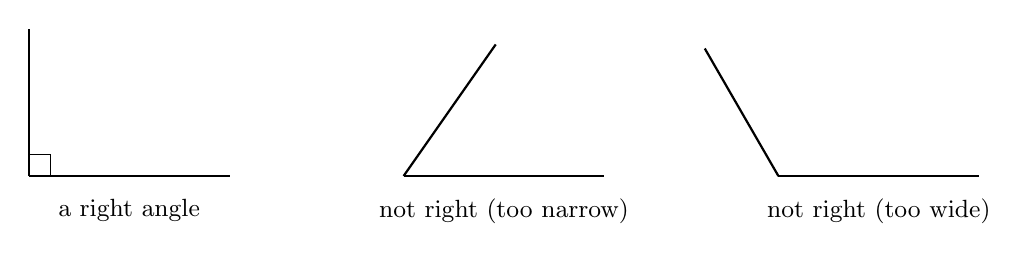
\begin{tikzpicture}[scale=0.85]
  \draw[thick] (0,0) -- (3,0);
  \draw[thick] (0,0) -- (0,2.2);
  \draw[thin] (0.32,0) -- (0.32,0.32) -- (0,0.32);
  \node[below, font=\small] at (1.5,-0.2) {a right angle};
  \begin{scope}[xshift=5.6cm]
  \draw[thick] (0,0) -- (3,0);
  \draw[thick] (0,0) -- (55:2.4);
  \node[below, font=\small] at (1.5,-0.2) {not right (too narrow)};
  \end{scope}
  \begin{scope}[xshift=11.2cm]
  \draw[thick] (0,0) -- (3,0);
  \draw[thick] (0,0) -- (120:2.2);
  \node[below, font=\small] at (1.5,-0.2) {not right (too wide)};
  \end{scope}
\end{tikzpicture}

{\small Only the first angle is right --- and only the little square
mark, or the set square, can certify it: eyes alone are easily
fooled.}
\end{omfigure}

\section{The shapes and their rules}

\begin{definition}[Square, rectangle, triangle]\label{def:g3:shapes:shapes}
\begin{itemize}
  \item A \emph{rectangle}\index{rectangle} has $4$ sides and $4$
        right angles; its opposite sides have the same length.
  \item A \emph{square}\index{square} is a rectangle whose $4$ sides
        all have the same length.
  \item A \emph{triangle}\index{triangle} has $3$ sides; a
        \emph{right triangle} has one right angle.
  \item A \emph{circle}\index{circle} is drawn with the compass: all
        its points are at the same distance (the \emph{radius}) from
        the \emph{center}.
\end{itemize}
\end{definition}

\begin{omfigure}
\begin{tikzpicture}[scale=0.72]
  % square
  \draw[thick] (0,0) rectangle (2,2);
  \foreach \c in {(0,0),(2,0),(0,2),(2,2)}
    \draw[thin] \c rectangle +(0.22,0.22);
  \draw (0.93,-0.07) -- (1.07,0.07);
  \draw (0.93,1.93) -- (1.07,2.07);
  \draw (-0.07,0.93) -- (0.07,1.07);
  \draw (1.93,0.93) -- (2.07,1.07);
  \node[below, font=\small] at (1,-0.3) {square};
  % rectangle
  \begin{scope}[xshift=3.8cm]
  \draw[thick] (0,0) rectangle (3,2);
  \foreach \c in {(0,0),(3,0),(0,2),(3,2)}
    \draw[thin] \c rectangle +(0.22,0.22);
  \node[below, font=\small] at (1.5,-0.3) {rectangle};
  \end{scope}
  % right triangle
  \begin{scope}[xshift=8.6cm]
  \draw[thick] (0,0) -- (2.6,0) -- (0,2) -- cycle;
  \draw[thin] (0.28,0) -- (0.28,0.28) -- (0,0.28);
  \node[below, font=\small] at (1.3,-0.3) {right triangle};
  \end{scope}
  % circle
  \begin{scope}[xshift=13.2cm]
  \draw[thick] (1,1) circle (1.1);
  \fill (1,1) circle (1.5pt);
  \draw[omDef] (1,1) -- (2.1,1) node[midway, above, font=\small]
    {radius};
  \node[below, font=\small] at (1,-0.3) {circle};
  \end{scope}
\end{tikzpicture}

{\small The shape gallery, with their marks: little squares for right
angles, small ticks for equal sides.}
\end{omfigure}

\begin{example}[Why marks matter]\label{ex:g3:shapes:marks}
A shape drawn slightly tilted can \emph{look} like a square without
being one. The marks tell the truth: $4$ right-angle squares $+$ $4$
tick marks $=$ a real square. When you draw, put the marks; when you
read a figure, trust only the marks and the given measures.
\end{example}

\section{Drawing on grid paper}

\begin{method}[Constructions on a grid]\label{met:g3:shapes:grid}
Grid paper offers free right angles: its lines are perpendicular.
\begin{enumerate}
  \item To draw a rectangle $5$ by $3$: choose a crossing point,
        count $5$ squares right, $3$ squares up, and close the shape
        along the grid lines;
  \item to check equal lengths, count squares;
  \item diagonal steps make tilted lines: going ``$1$ right, $1$ up''
        repeatedly draws a $45^\circ$ line.
\end{enumerate}
\end{method}

\begin{omfigure}
\begin{tikzpicture}[scale=0.5]
  \draw[gray!40, thin] (0,0) grid (13,5);
  \draw[very thick, omDef] (1,1) rectangle (6,4);
  \node[omDef, font=\small] at (3.5,2.5) {$5 \times 3$ rectangle};
  \draw[very thick, omThm] (8,1) -- (12,1) -- (8,4) -- cycle;
  \node[omThm, font=\small, below right] at (8.35,3.4) {right
  triangle};
\end{tikzpicture}

{\small Two constructions on the grid: the grid lines guarantee the
right angles.}
\end{omfigure}

\begin{example}[A construction program]\label{ex:g3:shapes:program}
A figure can be described by instructions:
``1. Draw a square $ABCD$ of side $4$ cm. 2. Draw the circle with
center $A$ passing through $B$.'' Following a program line by line,
anyone can redraw the same figure --- and writing one forces you to
name every point. Try it with a partner: one writes, the other
draws.
\end{example}

\section{Exercises}

\begin{exercise}[$\star$]\label{exo:g3:shapes:1}
In the classroom, find (without measuring) three right angles and
one angle that is not right. How can you \emph{check} each one?
\end{exercise}

\begin{exercise}[$\star$]\label{exo:g3:shapes:2}
Draw a rectangle of $6$ cm by $4$ cm with ruler and set square. Mark
its right angles and its equal sides.
\end{exercise}

\begin{exercise}[$\star$]\label{exo:g3:shapes:3}
Draw a square of side $5$ cm. How many right angles does it have?
How many equal sides? Mark everything.
\end{exercise}

\begin{exercise}[$\star$]\label{exo:g3:shapes:4}
On grid paper, draw: a $4 \times 4$ square; a $7 \times 2$
rectangle; a right triangle with legs of $3$ and $5$ squares.
\end{exercise}

\begin{exercise}[$\star$]\label{exo:g3:shapes:5}
True or false? Explain.
``Every square is a rectangle.'' \quad
``Every rectangle is a square.'' \quad
``A triangle can have two right angles.'' (Try to draw one!)
\end{exercise}

\begin{exercise}[$\star$]\label{exo:g3:shapes:6}
Draw a circle of radius $4$ cm. Mark its center $O$, a point $A$ on
the circle, and draw the radius $[OA]$. How long is $OA$? And if $B$
is another point of the circle, how long is $OB$?
\end{exercise}

\begin{exercise}[$\star$]\label{exo:g3:shapes:7}
Follow this program: ``1. Draw a rectangle $ABCD$ with $AB = 6$ cm
and $BC = 3$ cm. 2. Mark the point $M$ in the middle of $[AB]$.
3. Join $M$ to $C$ and to $D$.'' What shapes has the rectangle been
cut into?
\end{exercise}

\begin{exercise}[$\star$]\label{exo:g3:shapes:8}
Sort the shapes: which of these have at least one right angle?
A square; a (non-square) rectangle; a right triangle; a circle; the
letter L drawn with thick strokes.
\end{exercise}

\begin{exercise}[$\star\star$]\label{exo:g3:shapes:9}
On grid paper, draw a tilted square whose sides go ``$2$ right, $1$
up'' (and the matching turns). Count squares to convince yourself
the four sides have the same length.
\end{exercise}

\begin{exercise}[$\star\star$]\label{exo:g3:shapes:10}
Write a construction program (numbered instructions, named points)
for: a square of side $3$ cm sitting on top of a rectangle
$3$ cm $\times$ $2$ cm, like a house on its ground floor. Test your
program on a classmate.
\end{exercise}

\begin{exercise}[$\star\star$]\label{exo:g3:shapes:11}
How many squares can you find in a $3 \times 3$ grid of small
squares? (Count the $1 \times 1$, the $2 \times 2$ and the
$3 \times 3$ ones.)
\end{exercise}

\chapter{Measuring}\label{ch:g3:measure}

How long, how heavy, how much does it hold, how late is it? Measuring
turns the world into numbers --- provided everyone uses the same
units. This chapter presents the units of length, mass and capacity,
and teaches how to read a clock.

\section{Lengths}

\begin{definition}[Units of length]\label{def:g3:measure:length}
The basic unit of length is the \emph{meter} (m). For small lengths:
the centimeter (cm) and the millimeter (mm); for long distances: the
kilometer (km).
\[
1 \text{ m} = 100 \text{ cm}, \qquad
1 \text{ cm} = 10 \text{ mm}, \qquad
1 \text{ km} = 1\,000 \text{ m}.
\]
\end{definition}

\begin{omfigure}
\begin{tikzpicture}[scale=1.3]
  % ruler body extends past the marks so no numeral is clipped
  \draw[thick] (-0.35,0) rectangle (8.35,0.9);
  \foreach \i in {0,...,8} {
    \draw[thick] (\i,0.9) -- (\i,0.55);
    \node[font=\small] at (\i,0.32) {\i};
  }
  \foreach \i in {0,...,80} \draw (\i*0.1,0.9) -- (\i*0.1,0.72);
  \draw[omThm, very thick] (0,1.25) -- (3.6,1.25);
  \node[omThm, above, font=\small] at (1.8,1.3)
    {$3.6$ cm $= 3$ cm and $6$ mm};
\end{tikzpicture}

{\small Reading a ruler: big marks for centimeters, small marks for
millimeters. The object starts at the $0$ mark --- not at the edge of
the ruler! --- and ends at the $6$th small mark after the $3$.}
\end{omfigure}

\begin{example}[Choosing the right unit]\label{ex:g3:measure:choose}
An ant: about $5$ mm. A pencil: about $18$ cm. A door: about $2$ m.
A walk to the next village: about $3$ km. Giving ``the length of a
pencil is $18$'' means nothing --- the unit is part of the answer.
\end{example}

\begin{method}[Converting units]\label{met:g3:measure:convert}
To convert, multiply or divide by $10$, $100$ or $1\,000$:
\begin{enumerate}
  \item from a big unit to a small one, \emph{multiply}:
        $3$ m $= 3 \times 100 = 300$ cm;
  \item from a small unit to a big one, \emph{divide}:
        $250$ cm $= 250 \div 100 = 2$ m and $50$ cm;
  \item to add lengths, convert them to the \emph{same} unit first:
        $1$ m $+ 35$ cm $= 100 + 35 = 135$ cm.
\end{enumerate}
\end{method}

\section{Masses and capacities}

\begin{definition}[Units of mass and capacity]\label{def:g3:measure:mass}
Masses are measured in \emph{grams} (g) and \emph{kilograms} (kg),
capacities (how much a container holds) in \emph{liters} (L) and
\emph{centiliters} (cL):
\[
1 \text{ kg} = 1\,000 \text{ g},
\qquad
1 \text{ L} = 100 \text{ cL}.
\]
\end{definition}

\begin{example}\label{ex:g3:measure:mass}
A letter: about $20$ g. A bag of flour: $1$ kg. A bathtub: about
$150$ L. A glass: about $20$ cL. To balance a scale holding a
$1$ kg bag against $650$ g of apples, add $1\,000 - 650 = 350$ g on
the apples' side.
\end{example}

\section{Reading the clock}

\begin{method}[Reading the time]\label{met:g3:measure:clock}
On a clock with hands:
\begin{enumerate}
  \item the \emph{short} hand gives the hour: read the number it has
        passed last;
  \item the \emph{long} hand gives the minutes: each big mark is $5$
        minutes, so a long hand on the $3$ means $15$ minutes;
  \item after half past, one can also read ``to the next hour'':
        $10{:}50$ is ``ten to eleven''.
\end{enumerate}
\end{method}

\begin{omfigure}
\begin{tikzpicture}[scale=1.0]
  % clock 1: 3:00
  \draw[thick] (0,0) circle (1.3);
  \foreach \h in {1,...,12} {
    \node[font=\footnotesize] at ({90-\h*30}:1.05) {\h};
    \draw ({90-\h*30}:1.22) -- ({90-\h*30}:1.3);
  }
  \draw[very thick, omDef] (0,0) -- (0:0.65);
  \draw[thick, omThm] (0,0) -- (90:1.05);
  \node[below, font=\small] at (0,-1.55) {3:00};
  % clock 2: 7:30
  \begin{scope}[xshift=4.4cm]
  \draw[thick] (0,0) circle (1.3);
  \foreach \h in {1,...,12} {
    \node[font=\footnotesize] at ({90-\h*30}:1.05) {\h};
    \draw ({90-\h*30}:1.22) -- ({90-\h*30}:1.3);
  }
  \draw[very thick, omDef] (0,0) -- ({90-7.5*30}:0.65);
  \draw[thick, omThm] (0,0) -- (270:1.05);
  \node[below, font=\small] at (0,-1.55) {7:30};
  \end{scope}
  % clock 3: 10:50
  \begin{scope}[xshift=8.8cm]
  \draw[thick] (0,0) circle (1.3);
  \foreach \h in {1,...,12} {
    \node[font=\footnotesize] at ({90-\h*30}:1.05) {\h};
    \draw ({90-\h*30}:1.22) -- ({90-\h*30}:1.3);
  }
  \draw[very thick, omDef] (0,0) -- ({90-10.83*30}:0.65);
  \draw[thick, omThm] (0,0) -- ({90-10*30}:1.05);
  \node[below, font=\small] at (0,-1.55) {10:50};
  \end{scope}
\end{tikzpicture}

{\small Three clocks: short blue hand for hours, long red hand for
minutes. At 7:30 the hour hand sits \emph{between} 7 and 8; at 10:50
it is almost on the 11.}
\end{omfigure}

\begin{example}[Durations]\label{ex:g3:measure:duration}
The film starts at $14{:}40$ and ends at $16{:}10$. How long is it?
Count in two hops:
\begin{enumerate}
  \item from $14{:}40$ to $15{:}00$: $20$ minutes;
  \item from $15{:}00$ to $16{:}10$: $1$ hour $10$ minutes.
\end{enumerate}
Total: $1$ h $30$ min. Careful: an hour has $60$ minutes, so
$16{:}10$ minus $14{:}40$ cannot be computed like $1610 - 1440$!
\end{example}

\section{Exercises}

\begin{exercise}[$\star$]\label{exo:g3:measure:1}
Which unit would you use (mm, cm, m or km) for: the width of a nail;
the height of a classmate; the length of the schoolyard; the
distance between two towns?
\end{exercise}

\begin{exercise}[$\star$]\label{exo:g3:measure:2}
Convert: $5$ m into cm; \quad $70$ mm into cm; \quad $4$ km into m;
\quad $600$ cm into m.
\end{exercise}

\begin{exercise}[$\star$]\label{exo:g3:measure:3}
Measure with your ruler (to the nearest millimeter) the sides of a
triangle drawn by a classmate, and compute the total length of its
border.
\end{exercise}

\begin{exercise}[$\star$]\label{exo:g3:measure:4}
Compute, converting first: $2$ m $+ 45$ cm (in cm); \quad
$1$ km $+ 250$ m (in m); \quad $3$ cm $+ 8$ mm (in mm).
\end{exercise}

\begin{exercise}[$\star$]\label{exo:g3:measure:5}
Convert: $3$ kg into g; \quad $2\,500$ g into kg and g; \quad
$4$ L into cL; \quad $350$ cL into L and cL.
\end{exercise}

\begin{exercise}[$\star$]\label{exo:g3:measure:6}
A recipe needs $750$ g of flour. Mona has a $1$ kg bag. Does she have
enough? How much will be left?
\end{exercise}

\begin{exercise}[$\star$]\label{exo:g3:measure:7}
Read the times: the short hand is between $2$ and $3$, the long hand
on the $6$; the short hand on the $9$, the long hand on the $12$;
the short hand almost on the $5$, the long hand on the $10$.
\end{exercise}

\begin{exercise}[$\star$]\label{exo:g3:measure:8}
School starts at $8{:}30$ and the morning ends at $11{:}45$. How long
is the morning? (Count in hops, as in
\cref{ex:g3:measure:duration}.)
\end{exercise}

\begin{exercise}[$\star$]\label{exo:g3:measure:9}
The train leaves at $9{:}50$ and the ride lasts $45$ minutes. At what
time does it arrive? (Hop to $10{:}00$ first.)
\end{exercise}

\begin{exercise}[$\star\star$]\label{exo:g3:measure:10}
A bottle holds $1$ L. Paul fills glasses of $20$ cL. How many full
glasses can he pour? (Convert first.)
\end{exercise}

\begin{exercise}[$\star\star$]\label{exo:g3:measure:11}
Lena walks $600$ m to school, and back, every day. How many meters
does she walk in a $5$-day school week? Give the answer in meters,
then in kilometers.
\end{exercise}

\chapter{Solving Problems}\label{ch:g3:problems}

Knowing the four operations is one thing; knowing \emph{which one} a
story needs is another. This chapter gives a method for word
problems --- the same four steps every time --- and teaches how to
read information from tables and pictograms.

\section{The four steps}

\begin{method}[Solving a word problem]\label{met:g3:problems:steps}
\begin{enumerate}
  \item \emph{Read} the problem twice; say in your own words what is
        asked, and what is known.
  \item \emph{Choose} the operation: draw a quick sketch or a bar
        picture if the choice is not obvious.
  \item \emph{Compute}, in columns or mentally, with an estimate as a
        safety net.
  \item \emph{Answer} with a full sentence, including the unit ---
        and check the answer makes sense (a child does not weigh
        $300$ kg).
\end{enumerate}
\end{method}

\begin{example}[Which operation?]\label{ex:g3:problems:which}
The words hint at the operation, the sketch decides:
\begin{itemize}
  \item \emph{putting together / in all}: addition;
  \item \emph{taking away / how many more / what is missing}:
        subtraction;
  \item \emph{so many groups of so many / so many times}:
        multiplication;
  \item \emph{sharing fairly / how many groups}: division.
\end{itemize}
\end{example}

\begin{omfigure}
\begin{tikzpicture}[scale=0.62]
  % addition bar
  \draw[thick, fill=omDef!20] (0,0) rectangle (3.4,0.8);
  \draw[thick, fill=omThm!20] (3.4,0) rectangle (5.8,0.8);
  \node[font=\small] at (1.7,0.4) {$26$};
  \node[font=\small] at (4.6,0.4) {$17$};
  \draw[Stealth-Stealth] (0,-0.35) -- (5.8,-0.35);
  \node[below, font=\small] at (2.9,-0.4) {? in all: $26 + 17$};
  % comparison bar
  \begin{scope}[xshift=9.4cm]
  \draw[thick, fill=omDef!20] (0,0.9) rectangle (5.2,1.7);
  \node[font=\small] at (2.6,1.3) {$52$};
  \draw[thick, fill=omThm!20] (0,0) rectangle (3.5,0.8);
  \node[font=\small] at (1.75,0.4) {$35$};
  \draw[Stealth-Stealth] (3.5,0.4) -- (5.2,0.4);
  \node[below, font=\small] at (2.6,-0.15)
    {? more: $52 - 35$};
  \end{scope}
\end{tikzpicture}

{\small Bar pictures make the operation visible: parts side by side
call for an addition; two bars compared call for a subtraction.}
\end{omfigure}

\begin{example}[A two-step problem]\label{ex:g3:problems:twostep}
``Maya buys $3$ packs of $6$ bottles and drinks $2$ bottles. How many
bottles are left?''
\begin{enumerate}
  \item What is asked: the number of bottles remaining. Known: $3$
        packs of $6$; $2$ drunk.
  \item Sketch: $3$ groups of $6$, then take $2$ away. Two
        operations!
  \item Compute: $3 \times 6 = 18$, then $18 - 2 = 16$.
  \item Sentence: $16$ bottles are left.
\end{enumerate}
Never stop after the first operation: reread the question to see
whether the story is finished.
\end{example}

\begin{example}[A useless number]\label{ex:g3:problems:trap}
``A baker, who is $52$ years old, bakes $120$ rolls and sells $85$.
How many rolls are left?'' The age is there to distract you: the
answer only needs $120 - 85 = 35$ rolls. Before computing, always
sort the numbers: which ones does the question really use?
\end{example}

\section{Reading tables and pictograms}

\begin{example}[A table]\label{ex:g3:problems:table}
Books borrowed at the library:
\begin{center}
\renewcommand{\arraystretch}{1.3}
\begin{tabular}{l|cccc}
 & comics & novels & science & total \\
\hline
week 1 & $14$ & $9$ & $6$ & $29$ \\
week 2 & $11$ & $12$ & $8$ & $31$ \\
\end{tabular}
\end{center}
Reading: week 2, novels: $12$. Computing from the table: in the two
weeks together, $14 + 11 = 25$ comics were borrowed; the busiest
week was week 2 ($31 > 29$).
\end{example}

\begin{example}[A pictogram]\label{ex:g3:problems:pictogram}
In a pictogram, one symbol stands for a fixed amount --- read the
key first!

\begin{omfigure}
\begin{tikzpicture}[scale=0.62]
  \node[left, font=\small] at (0,2.4) {Monday};
  \foreach \i in {0,1,2} \fill[omDef] (0.5+\i*0.8,2.4) circle (0.26);
  \node[left, font=\small] at (0,1.2) {Tuesday};
  \foreach \i in {0,1,2,3,4} \fill[omDef] (0.5+\i*0.8,1.2) circle (0.26);
  \node[left, font=\small] at (0,0) {Wednesday};
  \foreach \i in {0,1} \fill[omDef] (0.5+\i*0.8,0) circle (0.26);
  \fill[omDef] (0.5+1.6,0) circle (0.26);
  \node[right, font=\small] at (5.4,1.2)
    {key: one dot $= 4$ cakes sold};
\end{tikzpicture}

{\small A pictogram: Monday shows $3$ dots, so $3 \times 4 = 12$
cakes; Tuesday $5$ dots, $20$ cakes; Wednesday $3$ dots, $12$
cakes.}
\end{omfigure}
\end{example}

\section{Exercises}

\begin{exercise}[$\star$]\label{exo:g3:problems:1}
For each story, just \emph{name} the operation (do not compute):
a flock of $48$ sheep joins a flock of $37$; \ $56$ cherries shared
among $7$ children; \ $9$ boxes of $8$ pencils; \ Ali had $71$ cards
and gave away $18$.
\end{exercise}

\begin{exercise}[$\star$]\label{exo:g3:problems:2}
Solve with the four steps: ``A parking lot has $246$ cars in the
morning; $158$ more arrive at noon. How many cars are there now?''
\end{exercise}

\begin{exercise}[$\star$]\label{exo:g3:problems:3}
Solve: ``A rope of $90$ m is cut into pieces of $9$ m. How many
pieces?''
\end{exercise}

\begin{exercise}[$\star$]\label{exo:g3:problems:4}
Solve: ``Tickets cost $8$ each. What do $26$ tickets cost?''
\end{exercise}

\begin{exercise}[$\star$]\label{exo:g3:problems:5}
Draw a bar picture, then solve: ``Emma has $64$ stickers, Hugo has
$29$ fewer. How many has Hugo?''
\end{exercise}

\begin{exercise}[$\star$]\label{exo:g3:problems:6}
Two steps: ``A crate holds $45$ apples. A grocer receives $6$ crates
and sells $178$ apples. How many apples remain?''
\end{exercise}

\begin{exercise}[$\star$]\label{exo:g3:problems:7}
Using the table of \cref{ex:g3:problems:table}: how many science
books were borrowed in the two weeks together? How many more novels
in week 2 than in week 1?
\end{exercise}

\begin{exercise}[$\star$]\label{exo:g3:problems:8}
Using the pictogram of \cref{ex:g3:problems:pictogram}: how many
cakes were sold in the three days together? On which day were the
most cakes sold?
\end{exercise}

\begin{exercise}[$\star$]\label{exo:g3:problems:9}
This problem has a useless number --- find it, then solve: ``A
$210$-page book costs $12$. Leo reads $35$ pages a day. How many
days does he need to finish the book?''
\end{exercise}

\begin{exercise}[$\star\star$]\label{exo:g3:problems:10}
``A family of $2$ adults and $3$ children visits the museum. Adult
tickets cost $9$, children tickets $4$. They pay with a $50$ bill.
How much change do they get?'' (Three steps: adults, children, then
the change.)
\end{exercise}

\begin{exercise}[$\star\star$]\label{exo:g3:problems:11}
Make up your own two-step problem whose answer is $100$, write its
solution with the four steps, and test it on a classmate.
\end{exercise}


% ============================================================================
% Grade 4 — shared structure (language-agnostic).
% Bodies: parts/grade-4/<file>.tex (en) or parts/grade-4/<lang>/<file>.tex
% ============================================================================
\part{\omstr{part.grade4}}

\ominput{grade-4}{01-large-numbers}
\ominput{grade-4}{02-multiplication}
\ominput{grade-4}{03-division}
\ominput{grade-4}{04-first-fractions}
\ominput{grade-4}{05-tenths-and-hundredths}
\ominput{grade-4}{06-lines-and-polygons}
\ominput{grade-4}{07-symmetry}
\ominput{grade-4}{08-measures-and-perimeter}

% ============================================================================
% Grade 5 (age 10–11) — fifth and last year of primary school.
%
% One chapter per file. Solutions live in solutions/, one file per chapter,
% same numbering.
% ============================================================================
\part{Grade 5 (Age 10--11)}

\chapter{Decimal Numbers}\label{ch:g5:decimals}

Tenths and hundredths appeared in \cref{ch:g4:decimals}; adding one
more level, thousandths, completes the decimal system. This chapter
consolidates reading, decomposing and --- above all --- comparing
decimal numbers without falling into their famous traps.

\section{Down to thousandths}

\begin{definition}[Decimal places]\label{def:g5:decimals:places}
After the decimal point come the tenths, the hundredths, the
thousandths --- each worth ten times less than the one before:
\[
4.362 = 4 + \frac{3}{10} + \frac{6}{100} + \frac{2}{1000}
= \frac{4\,362}{1000}.
\]
\end{definition}

\begin{omfigure}
\begin{tikzpicture}[scale=0.9]
  \draw (0,0) grid[xstep=2.3, ystep=0.85] (9.2,1.7);
  \node[font=\small] at (1.15,1.275) {units};
  \node[font=\small] at (3.45,1.275) {tenths};
  \node[font=\small] at (5.75,1.275) {hundredths};
  \node[font=\small] at (8.05,1.275) {thousandths};
  \node[font=\large, omDef] at (1.15,0.425) {$4$};
  \node[font=\large, omThm] at (3.45,0.425) {$3$};
  \node[font=\large, omThm] at (5.75,0.425) {$6$};
  \node[font=\large, omThm] at (8.05,0.425) {$2$};
  \fill (2.3,0.06) circle (2.5pt);
\end{tikzpicture}

{\small The place-value table of $4.362$: whole part in blue, decimal
part in red, the point between units and tenths.}
\end{omfigure}

\begin{example}[Many readings, one number]\label{ex:g5:decimals:readings}
$4.362$ can be read ``four point three six two'', or ``four and
$362$ thousandths'', or decomposed as $4 + 0.3 + 0.06 + 0.002$. And
padding with final zeros changes nothing: $4.362 = 4.3620$. But
$4.362 \neq 4.0362$: a zero \emph{inside} pushes every digit to a
smaller place.
\end{example}

\begin{example}[Where is it on the line?]\label{ex:g5:decimals:line}
To place $4.362$: between $4$ and $5$; zooming, between $4.3$ and
$4.4$; zooming again, between $4.36$ and $4.37$, closer to $4.36$.
Each decimal digit is one more level of zoom.
\end{example}

\begin{omfigure}
\begin{tikzpicture}[scale=1.15]
  \draw[-Stealth] (-0.2,1.6) -- (10.4,1.6);
  \foreach \i in {0,...,10} \draw (\i,1.52) -- (\i,1.68);
  \node[below, font=\small] at (0,1.5) {$4$};
  \node[below, font=\small] at (10,1.5) {$5$};
  \node[below, font=\small] at (3,1.5) {$4.3$};
  \node[below, font=\small] at (4,1.5) {$4.4$};
  \fill[omThm] (3.62,1.6) circle (1.7pt);
  \draw[omExo, thin] (3,1.45) -- (0,0.15);
  \draw[omExo, thin] (4,1.45) -- (10,0.15);
  \draw[-Stealth] (-0.2,0) -- (10.4,0);
  \foreach \i in {0,...,10} \draw (\i,-0.08) -- (\i,0.08);
  \node[below, font=\small] at (0,-0.1) {$4.3$};
  \node[below, font=\small] at (10,-0.1) {$4.4$};
  \node[below, font=\small] at (6,-0.1) {$4.36$};
  \fill[omThm] (6.2,0) circle (1.7pt)
    node[above, font=\small] {$4.362$};
\end{tikzpicture}

{\small Zooming on the number line: the stretch from $4.3$ to $4.4$,
magnified, is itself cut into ten hundredths --- and $4.362$ sits
just past $4.36$.}
\end{omfigure}

\section{Comparing decimals}

\begin{method}[Comparing two decimals]\label{met:g5:decimals:compare}
\begin{enumerate}
  \item Compare the whole parts: $6.1 > 5.987$.
  \item Equal whole parts: compare the decimal parts digit by digit
        from the point --- tenths, then hundredths, then
        thousandths;
  \item padding with final zeros makes the comparison fair:
        $2.5$ vs $2.48$ becomes $2.50$ vs $2.48$, and $50 > 48$
        hundredths.
\end{enumerate}
The trap, one last time: \emph{a longer decimal part does not mean a
bigger number} --- $2.48$ has more digits than $2.5$ and is smaller.
\end{method}

\begin{example}\label{ex:g5:decimals:order}
Order $7.3$; $7.09$; $7.31$; $7.299$. Pad to three decimals:
$7.300$; $7.090$; $7.310$; $7.299$. Then
\[
7.09 < 7.299 < 7.3 < 7.31 .
\]
Note $7.299 < 7.3$ even though $299$ looks big: $299$ thousandths
against $300$ thousandths.
\end{example}

\begin{example}[Squeezing between two decimals]\label{ex:g5:decimals:between}
Is there a number between $5.7$ and $5.8$? Yes, plenty: $5.75$,
$5.71$, $5.799$\,\dots\ Between $5.79$ and $5.8$? Again plenty:
$5.795$, for one. Between two different decimals, one can
\emph{always} squeeze another --- there is no ``next'' decimal
number.
\end{example}

\section{Rounding decimals}

\begin{definition}[Rounding]\label{def:g5:decimals:round}
To round to the unit (or tenth, or hundredth), look at the next
digit: $5$ or more rounds up, otherwise round down. So $4.362$
rounds to $4$ (unit), to $4.4$ (tenth), to $4.36$ (hundredth).
\end{definition}

\begin{example}[Money rounds to cents]\label{ex:g5:decimals:money}
A price computed as $7.4983$ is displayed as $7.50$: real-life
amounts are rounded to the hundredth. Note the cascade: $7.4983 \to
7.50$, where the $49$ became $50$ --- rounding can ripple through
several digits.
\end{example}

\section{Exercises}

\begin{exercise}[$\star$]\label{exo:g5:decimals:1}
Write as a decimal number: $5 + \frac{2}{10} + \frac{7}{1000}$;
\quad $\frac{85}{100}$; \quad $\frac{4\,507}{1000}$; \quad ``twelve
and nine thousandths''.
\end{exercise}

\begin{exercise}[$\star$]\label{exo:g5:decimals:2}
In $27.418$: what does the $4$ count? The $8$? Decompose the number
as in \cref{def:g5:decimals:places}.
\end{exercise}

\begin{exercise}[$\star$]\label{exo:g5:decimals:3}
True or false? Explain with places.
$3.60 = 3.6$; \quad $0.5 = 0.05$; \quad $2.070 = 2.07$; \quad
$1.3 = 1.03$.
\end{exercise}

\begin{exercise}[$\star$]\label{exo:g5:decimals:4}
Copy and complete with $<$, $>$ or $=$:
\[
4.8 \;?\; 4.79, \qquad
0.302 \;?\; 0.32, \qquad
6.5 \;?\; 6.500, \qquad
9.09 \;?\; 9.1 .
\]
\end{exercise}

\begin{exercise}[$\star$]\label{exo:g5:decimals:5}
Order from smallest to biggest: $3.14$; \ $3.4$; \ $3.041$; \
$3.104$; \ $3.41$.
\end{exercise}

\begin{exercise}[$\star$]\label{exo:g5:decimals:6}
Between which two whole numbers does each number lie? Between which
two numbers with one decimal? \quad $6.83$; \quad $0.492$; \quad
$12.06$.
\end{exercise}

\begin{exercise}[$\star$]\label{exo:g5:decimals:7}
Round $8.276$: to the unit; to the tenth; to the hundredth. Round
$3.95$ to the tenth.
\end{exercise}

\begin{exercise}[$\star$]\label{exo:g5:decimals:8}
Give a number strictly between: $2.6$ and $2.7$; \quad $0.41$ and
$0.42$; \quad $5.99$ and $6$.
\end{exercise}

\begin{exercise}[$\star$]\label{exo:g5:decimals:9}
The heights of four plants are $0.85$ m, $1.2$ m, $0.9$ m and
$1.02$ m. Order them from shortest to tallest.
\end{exercise}

\begin{exercise}[$\star\star$]\label{exo:g5:decimals:10}
Lucie says: ``$7.12 > 7.9$ because $12 > 9$''. Correct her mistake,
comparing tenths first.
\end{exercise}

\begin{exercise}[$\star\star$]\label{exo:g5:decimals:11}
Find all the numbers with exactly two decimal digits that round to
$6.4$ when rounded to the tenth. What are the smallest and the
biggest?
\end{exercise}

\chapter{Computing with Decimals}\label{ch:g5:decimalops}

Decimal numbers add, subtract and multiply almost like whole numbers
--- the whole art is knowing where the point goes. This chapter
covers the column methods and the magic of multiplying or dividing by
$10$, $100$, $1000$. (Multiplying two decimals together waits for
\cref{ch:g6:decimals}.)

\section{Adding and subtracting}

\begin{method}[Columns with a point]\label{met:g5:decimalops:addsub}
\begin{enumerate}
  \item Write the numbers with the \emph{decimal points aligned}
        (then units are under units, tenths under tenths);
  \item pad the shorter decimal part with zeros;
  \item add or subtract as with whole numbers;
  \item drop the point of the result straight down.
\end{enumerate}
\end{method}

\begin{example}\label{ex:g5:decimalops:addsub}
$27.5 + 3.86$ (pad $27.5 = 27.50$):
\[
\begin{array}{r}
2\,7.5\,0 \\
+\ \ \ 3.8\,6 \\
\hline
3\,1.3\,6
\end{array}
\qquad\qquad
\begin{array}{r}
1\,2.4\,0 \\
-\ \ \ 5.6\,5 \\
\hline
\ \ \,6.7\,5
\end{array}
\]
For the subtraction ($12.4 - 5.65$): pad, borrow as usual, and check
by adding back: $6.75 + 5.65 = 12.4$.
\end{example}

\begin{example}[Mental complements]\label{ex:g5:decimalops:complement}
What must be added to $7.6$ to reach $10$? Climb: $7.6 \to 8$ is
$0.4$, then $8 \to 10$ is $2$: the complement is $2.4$. Handy for
change: pay $10$ for a $7.60$ item, get $2.40$ back.
\end{example}

\section{Ten times bigger, ten times smaller}

\begin{proposition}[Times and divided by 10, 100, 1000]\label{prop:g5:decimalops:shift}
Multiplying by $10$ makes each digit worth ten times more: the
digits slide one place left --- which looks like the \emph{point
moving one place right}. Dividing does the opposite:
\[
3.47 \times 10 = 34.7, \qquad
3.47 \times 100 = 347, \qquad
52.1 \div 10 = 5.21, \qquad
6 \div 100 = 0.06 .
\]
\end{proposition}
\admitted

\begin{omfigure}
\begin{tikzpicture}[scale=0.9]
  \draw (0,0) grid[xstep=1.5, ystep=0.75] (6.0,2.25);
  \node[font=\small] at (0.75,2.6) {tens};
  \node[font=\small] at (2.25,2.6) {units};
  \node[font=\small] at (3.75,2.6) {tenths};
  \node[font=\small] at (5.25,2.6) {hundredths};
  \node[font=\normalsize, omExo] at (2.25,1.85) {$3$};
  \node[font=\normalsize, omExo] at (3.75,1.85) {$4$};
  \node[font=\normalsize, omExo] at (5.25,1.85) {$7$};
  \node[font=\normalsize, omDef] at (0.75,1.1) {$3$};
  \node[font=\normalsize, omDef] at (2.25,1.1) {$4$};
  \node[font=\normalsize, omDef] at (3.75,1.1) {$7$};
  \node[right, font=\small] at (6.2,1.85) {$3.47$};
  \node[right, font=\small, omDef] at (6.2,1.1)
    {$3.47 \times 10 = 34.7$};
  \draw[-Stealth, omDef, thick] (4.4,1.7) -- (3.1,1.25);
\end{tikzpicture}

{\small Multiplying by $10$: every digit climbs one place to the
left. The point does not really move --- the digits do.}
\end{omfigure}

\begin{example}[Conversions again]\label{ex:g5:decimalops:convert}
Units of measure are powers of ten apart, so conversions are just
these shifts: $2.35$ m $= 235$ cm ($\times 100$); $470$ g
$= 0.47$ kg ($\div 1000$); $1.5$ L $= 150$ cL.
\end{example}

\section{Multiplying a decimal by a whole number}

\begin{method}[Decimal times whole]\label{met:g5:decimalops:mult}
Compute as if there were no point, then give the result as many
decimal digits as the decimal factor:
\[
4.35 \times 6: \quad 435 \times 6 = 2\,610
\ \to\ 4.35 \times 6 = 26.10 = 26.1 .
\]
Estimate to place the point with confidence: $4.35$ is close to
$4$, and $4 \times 6 = 24$ --- so $26.1$, not $2.61$ nor $261$.
\end{method}

\begin{example}[Repeated addition still works]\label{ex:g5:decimalops:mult}
$0.75 \times 4 = 0.75 + 0.75 + 0.75 + 0.75 = 3$: four quarters make
a whole, in decimal clothing. Multiplying by a whole number is still
``so many times''.
\end{example}

\begin{example}[Shopping]\label{ex:g5:decimalops:shopping}
Three notebooks at $2.45$ each and a pen at $1.20$:
\begin{enumerate}
  \item notebooks: $2.45 \times 3 = 7.35$;
  \item total: $7.35 + 1.20 = 8.55$;
  \item change from $10$: $10 - 8.55 = 1.45$.
\end{enumerate}
\end{example}

\section{Exercises}

\begin{exercise}[$\star$]\label{exo:g5:decimalops:1}
Compute in columns: $45.7 + 8.93$; \quad $16.25 + 3.75$; \quad
$0.86 + 12.4$.
\end{exercise}

\begin{exercise}[$\star$]\label{exo:g5:decimalops:2}
Compute in columns and check: $9.4 - 2.72$; \quad $20 - 13.45$;
\quad $6.03 - 5.9$.
\end{exercise}

\begin{exercise}[$\star$]\label{exo:g5:decimalops:3}
Mental complements to $10$ (as in
\cref{ex:g5:decimalops:complement}): $6.2$; \quad $3.75$; \quad
$9.99$.
\end{exercise}

\begin{exercise}[$\star$]\label{exo:g5:decimalops:4}
Compute without columns:
\[
7.24 \times 10, \qquad
0.58 \times 100, \qquad
34.5 \div 10, \qquad
7 \div 100, \qquad
0.3 \times 1000 .
\]
\end{exercise}

\begin{exercise}[$\star$]\label{exo:g5:decimalops:5}
Convert: $4.05$ m in cm; \quad $325$ cm in m; \quad $0.6$ kg in g;
\quad $85$ cL in L.
\end{exercise}

\begin{exercise}[$\star$]\label{exo:g5:decimalops:6}
Estimate first, then compute: $6.2 \times 4$; \quad
$3.45 \times 8$; \quad $12.5 \times 6$.
\end{exercise}

\begin{exercise}[$\star$]\label{exo:g5:decimalops:7}
One lap of a track measures $0.4$ km. How long are $7$ laps? And
$25$ laps?
\end{exercise}

\begin{exercise}[$\star$]\label{exo:g5:decimalops:8}
Lea buys $2$ baguettes at $1.15$ each and a cake at $12.60$. She
pays with a $20$ bill. Compute her total and her change.
\end{exercise}

\begin{exercise}[$\star$]\label{exo:g5:decimalops:9}
A bottle holds $1.5$ L. How many liters in a pack of $6$ bottles?
A family drinks $0.75$ L per day: for how many days does one pack
last? (How many times does $0.75$ fit in $9$?)
\end{exercise}

\begin{exercise}[$\star\star$]\label{exo:g5:decimalops:10}
Milo computes $5.6 \times 3 = 15.18$, reasoning ``$5 \times 3 = 15$
and $6 \times 3 = 18$''. Use an estimate to show the answer must be
wrong, then compute correctly.
\end{exercise}

\begin{exercise}[$\star\star$]\label{exo:g5:decimalops:11}
A runner's four laps took $65.4$ s, $64.9$ s, $65.0$ s and
$66.1$ s.
\begin{enumerate}
  \item Compute the total time of the four laps.
  \item The record for four laps is $260$ s. Did she beat it? By how
        much?
\end{enumerate}
\end{exercise}

\chapter{Fractions as Numbers}\label{ch:g5:fractions}

A fraction is not just a picture of a pie: it is a genuine
\emph{number}, with a place on the number line --- sometimes the very
same place as a decimal number. This chapter connects the two
worlds. (The full rules of fraction arithmetic come in
\cref{ch:g6:fractions} and beyond.)

\section{Fractions on the line, again}

\begin{example}[Placing and reading]\label{ex:g5:fractions:place}
On a line cut in fifths, $\frac{7}{5}$ is $7$ steps from $0$: past
$1$ (which is $\frac55$), at $1 + \frac25$. Every fraction lives
somewhere on the line; bigger numerator (same denominator) means
further right.
\end{example}

\begin{proposition}[Same point, many names]\label{prop:g5:fractions:equal}
Cutting every part in two (or three\,\dots) does not move the
point:
\[
\frac{1}{2} = \frac{2}{4} = \frac{3}{6} = \frac{5}{10},
\qquad
\frac{2}{3} = \frac{4}{6} = \frac{20}{30}.
\]
Multiplying (or dividing) the numerator and the denominator by the
same number gives another name of the same fraction.
\end{proposition}
\admitted

\begin{omfigure}
\begin{tikzpicture}[scale=0.62]
  \foreach \i in {0,1} \draw[omExo] (\i*4,0) rectangle (\i*4+4,1.0);
  \fill[omDef!40] (0.06,0.06) rectangle (3.94,0.94);
  \draw[thick] (0,0) rectangle (8,1.0);
  \node[right, font=\small] at (8.3,0.5) {$\frac12$};
  \begin{scope}[yshift=-1.7cm]
  \foreach \i in {0,...,3} \draw[omExo] (\i*2,0) rectangle (\i*2+2,1.0);
  \fill[omDef!40] (0.06,0.06) rectangle (1.94,0.94);
  \fill[omDef!40] (2.06,0.06) rectangle (3.94,0.94);
  \draw[thick] (0,0) rectangle (8,1.0);
  \node[right, font=\small] at (8.3,0.5) {$\frac24$};
  \end{scope}
  \begin{scope}[yshift=-3.4cm]
  \foreach \i in {0,...,9} \draw[omExo] (\i*0.8,0) rectangle
    (\i*0.8+0.8,1.0);
  \foreach \i in {0,...,4} \fill[omDef!40] (\i*0.8+0.05,0.06)
    rectangle (\i*0.8+0.75,0.94);
  \draw[thick] (0,0) rectangle (8,1.0);
  \node[right, font=\small] at (8.3,0.5) {$\frac{5}{10}$};
  \end{scope}
\end{tikzpicture}

{\small Three bars, three names, one amount: $\frac12 = \frac24 =
\frac{5}{10}$.}
\end{omfigure}

\section{Fractions and decimals}

\begin{proposition}[Fractions with decimal names]\label{prop:g5:fractions:decimal}
Fractions of tenths, hundredths, thousandths \emph{are} decimal
numbers:
\[
\frac{3}{10} = 0.3, \qquad \frac{27}{100} = 0.27 .
\]
Some other fractions also have decimal names, found by switching to
tenths or hundredths:
\[
\frac{1}{2} = \frac{5}{10} = 0.5, \qquad
\frac{1}{4} = \frac{25}{100} = 0.25, \qquad
\frac{3}{4} = 0.75, \qquad
\frac{1}{5} = \frac{2}{10} = 0.2 .
\]
But not all: $\frac13 = 0.333\dots$ never ends --- the fraction is
its only exact name.
\end{proposition}
\admitted

\begin{omfigure}
\begin{tikzpicture}[scale=1.55]
  \draw[-Stealth] (-0.2,0) -- (7.6,0);
  \foreach \i in {0,...,28} \draw ({\i*0.25},-0.05) -- ({\i*0.25},0.05);
  \foreach \i in {0,4,...,28} \draw ({\i*0.25},-0.09) -- ({\i*0.25},0.09);
  \foreach \x in {0,...,7} \node[below, font=\small] at (\x,-0.1) {$\x$};
  \fill[omDef] (0.5,0) circle (1.6pt)
    node[above, font=\small] {$\frac12 = 0.5$};
  \fill[omThm] (2.75,0) circle (1.6pt)
    node[above, font=\small] {$\frac{11}{4} = 2.75$};
  \fill[omMeth] (6.25,0) circle (1.6pt)
    node[above, font=\small] {$\frac{25}{4} = 6.25$};
\end{tikzpicture}

{\small One line, two languages: each point can carry a fraction name
and a decimal name.}
\end{omfigure}

\begin{example}[Choosing the handier name]\label{ex:g5:fractions:choose}
To pay three quarters of $12$: the fraction name is handier,
$\frac34$ of $12$ is $9$. To compare $\frac34$ and $0.8$: the
decimal name is handier, $0.75 < 0.8$. Being bilingual pays off.
\end{example}

\section{Comparing fractions}

\begin{method}[Three comparison tools]\label{met:g5:fractions:compare}
\begin{enumerate}
  \item \emph{Same denominator}: more parts wins,
        $\frac57 > \frac37$;
  \item \emph{same numerator}: bigger parts win, so \emph{smaller}
        denominator wins: $\frac35 > \frac38$ (fifths are bigger
        than eighths);
  \item \emph{landmarks}: compare each to $\frac12$ or to $1$:
        $\frac38 < \frac12 < \frac59$, so $\frac38 < \frac59$.
\end{enumerate}
\end{method}

\begin{example}\label{ex:g5:fractions:compare}
Who ate more pizza: Ali with $\frac58$ or Bea with $\frac54$? Bea's
fraction is bigger than $1$ (five quarters is more than one whole
pizza), Ali's is smaller than $1$: Bea ate more --- more than a
whole pizza, in fact.
\end{example}

\section{Exercises}

\begin{exercise}[$\star$]\label{exo:g5:fractions:1}
Draw a number line cut in fifths from $0$ to $2$, and place:
$\frac25$; \ $\frac55$; \ $\frac85$; \ $\frac{10}{5}$.
\end{exercise}

\begin{exercise}[$\star$]\label{exo:g5:fractions:2}
Complete the equal names:
$\frac12 = \frac{?}{8}$; \quad
$\frac34 = \frac{?}{8}$; \quad
$\frac{2}{5} = \frac{4}{?}$; \quad
$\frac{6}{9} = \frac{2}{?}$.
\end{exercise}

\begin{exercise}[$\star$]\label{exo:g5:fractions:3}
Which fractions name whole numbers? Give the whole number when so:
$\frac82$; \quad $\frac{9}{4}$; \quad $\frac{15}{3}$; \quad
$\frac{20}{5}$.
\end{exercise}

\begin{exercise}[$\star$]\label{exo:g5:fractions:4}
Write as decimals: $\frac{7}{10}$; \quad $\frac{41}{100}$; \quad
$\frac12$; \quad $\frac34$; \quad $\frac15$.
\end{exercise}

\begin{exercise}[$\star$]\label{exo:g5:fractions:5}
Write as fractions (tenths or hundredths): $0.9$; \quad $0.13$;
\quad $2.5$; \quad $0.75$ (then give its quarter name).
\end{exercise}

\begin{exercise}[$\star$]\label{exo:g5:fractions:6}
Compare, naming the tool used
(\cref{met:g5:fractions:compare}):
\[
\frac47 \;?\; \frac67, \qquad
\frac35 \;?\; \frac37, \qquad
\frac25 \;?\; \frac{7}{12}, \qquad
\frac98 \;?\; \frac{11}{12} .
\]
\end{exercise}

\begin{exercise}[$\star$]\label{exo:g5:fractions:7}
Order with the decimal names: $\frac12$; \ $0.4$; \ $\frac34$; \
$0.6$; \ $\frac15$.
\end{exercise}

\begin{exercise}[$\star$]\label{exo:g5:fractions:8}
A quarter of the students of a class of $28$ play an instrument, and
half play a sport. How many students is each? Which group is bigger?
\end{exercise}

\begin{exercise}[$\star$]\label{exo:g5:fractions:9}
Match each fraction with a time: $\frac14$ h, $\frac12$ h,
$\frac34$ h, $\frac{1}{60}$ h --- to $30$ min, $45$ min, $1$ min,
$15$ min.
\end{exercise}

\begin{exercise}[$\star\star$]\label{exo:g5:fractions:10}
Tom drank $\frac35$ of his $50$ cL bottle; Ana drank $\frac12$ of
her $60$ cL bottle. Who drank more? (Compute both amounts in cL ---
comparing the bare fractions is not enough here, and say why.)
\end{exercise}

\begin{exercise}[$\star\star$]\label{exo:g5:fractions:11}
Give a fraction strictly between $\frac12$ and $1$; then one
strictly between $\frac12$ and $\frac34$. (Decimal names may
help.)
\end{exercise}

\chapter{Division and Multiples}\label{ch:g5:division}

Long division learned in \cref{ch:g4:division} gets two upgrades:
two-digit divisors, and quotients that continue past the point ---
$3 \div 4$ finally gets an answer, $0.75$. The chapter ends with
multiples, divisors and the first divisibility shortcuts.

\section{Dividing by a two-digit number}

\begin{method}[Two-digit divisors]\label{met:g5:division:twodigits}
Same method as before, with one extra skill: guessing how many times
the divisor fits. Write a small table of multiples of the divisor
first. For $986 \div 23$ (multiples of 23: 23, 46, 69, 92, 115,
138, 161, 184, 207):
\begin{enumerate}
  \item $98$ tens: $23 \times 4 = 92$ fits, $23 \times 5 = 115$ does
        not: digit $4$, remainder $6$;
  \item bring down the $6$: $66$: $23 \times 2 = 46$ fits: digit
        $2$, remainder $20$;
  \item quotient $42$, remainder $20$. Check:
        $23 \times 42 + 20 = 966 + 20 = 986$.
\end{enumerate}
\end{method}

\section{Decimal quotients}

\begin{example}[The division that refuses to stop at the remainder]\label{ex:g5:division:decimal}
Share $3$ pizzas among $4$ children: $3 \div 4$ has quotient $0$ and
remainder $3$ --- useless! Continue the division past the point:
\begin{enumerate}
  \item $3$ units $= 30$ tenths; $30 \div 4$: $7$ tenths, remainder
        $2$ tenths;
  \item $2$ tenths $= 20$ hundredths; $20 \div 4 = 5$ hundredths,
        remainder $0$.
\end{enumerate}
So $3 \div 4 = 0.75$: each child gets $0.75$ pizza --- three
quarters, as the fraction language already knew
(\cref{prop:g5:fractions:decimal}).
\end{example}

\begin{method}[Continuing a division past the point]\label{met:g5:division:continue}
When the units are exhausted and a remainder is left:
\begin{enumerate}
  \item write the decimal point in the quotient;
  \item append a zero to the remainder (units become tenths, tenths
        become hundredths\,\dots) and keep dividing;
  \item stop when the remainder is $0$ --- or when the digits start
        repeating forever, like $1 \div 3 = 0.333\dots$: then give a
        rounded value.
\end{enumerate}
\end{method}

\begin{example}\label{ex:g5:division:continue}
$27 \div 6$: quotient $4$, remainder $3$; point; $30$ tenths
$\div\ 6 = 5$: so $27 \div 6 = 4.5$. \quad
$22 \div 8$: $2$, remainder $6$; then $60 \div 8 = 7$ r $4$;
then $40 \div 8 = 5$: so $22 \div 8 = 2.75$.
\end{example}

\section{Multiples and divisors}

\begin{definition}[Multiple, divisor]\label{def:g5:division:multiple}
The \emph{multiples}\index{multiple} of $6$ are its table continued
forever: $0, 6, 12, 18, 24, \dots$ When $24$ is a multiple of $6$,
one also says that $6$ is a \emph{divisor}\index{divisor} of $24$,
or that $24$ is \emph{divisible} by $6$: the division
$24 \div 6$ leaves no remainder.
\end{definition}

\begin{proposition}[Divisibility shortcuts]\label{prop:g5:division:criteria}
Without dividing, a number is divisible:
\begin{itemize}
  \item by $2$ when its last digit is $0$, $2$, $4$, $6$ or $8$
        (the even numbers);
  \item by $5$ when its last digit is $0$ or $5$;
  \item by $10$ when its last digit is $0$;
  \item by $3$ when the \emph{sum of its digits} is divisible by
        $3$ (e.g.\ $741$: $7 + 4 + 1 = 12$, divisible --- and indeed
        $741 = 3 \times 247$).
\end{itemize}
\end{proposition}
\admitted

\begin{omfigure}
\begin{tikzpicture}[scale=0.5]
  \foreach \n in {0,...,29} {
    \pgfmathtruncatemacro{\r}{int(\n/10)}
    \pgfmathtruncatemacro{\c}{mod(\n,10)}
    \pgfmathtruncatemacro{\lbl}{\n+1}
    \pgfmathtruncatemacro{\mtwo}{mod(\lbl,2)}
    \pgfmathtruncatemacro{\mthree}{mod(\lbl,3)}
    \ifnum\mtwo=0
      \fill[omDef!25] (\c,-\r) ++(-0.45,-0.45) rectangle ++(0.9,0.9);
    \fi
    \ifnum\mthree=0
      \draw[omThm, thick] (\c,-\r) circle (0.42);
    \fi
    \node[font=\footnotesize] at (\c,-\r) {\lbl};
  }
  \node[font=\small, below] at (4.5,-2.8)
    {blue squares: multiples of $2$;\ \ red circles: multiples of
    $3$;\ \ both: multiples of $6$};
\end{tikzpicture}

{\small The numbers $1$ to $30$: multiples of $2$ and of $3$ make
patterns --- and the numbers wearing both marks ($6$, $12$, $18$,
$24$, $30$) are exactly the multiples of $6$.}
\end{omfigure}

\begin{example}\label{ex:g5:division:criteria}
Is $534$ divisible by $2$? Ends in $4$: yes. By $5$? No. By $3$?
$5 + 3 + 4 = 12$: yes. So $534$ is divisible by $6$ as well (by $2$
\emph{and} by $3$) --- check: $534 = 6 \times 89$.
\end{example}

\section{Exercises}

\begin{exercise}[$\star$]\label{exo:g5:division:1}
Compute the long divisions (table of multiples first):
$851 \div 23$; \quad $704 \div 32$.
\end{exercise}

\begin{exercise}[$\star$]\label{exo:g5:division:2}
Compute the exact decimal quotients: $9 \div 2$; \quad $27 \div 4$;
\quad $33 \div 5$; \quad $21 \div 8$.
\end{exercise}

\begin{exercise}[$\star$]\label{exo:g5:division:3}
Four friends share a $54$ restaurant bill equally. How much does
each pay? (Continue past the point.)
\end{exercise}

\begin{exercise}[$\star$]\label{exo:g5:division:4}
Compute $10 \div 3$, continuing three digits past the point. What do
you observe? Give the value rounded to the hundredth.
\end{exercise}

\begin{exercise}[$\star$]\label{exo:g5:division:5}
List: the multiples of $7$ up to $70$; the divisors of $18$; the
divisors of $24$.
\end{exercise}

\begin{exercise}[$\star$]\label{exo:g5:division:6}
Divisible by $2$? by $5$? by $10$? by $3$? Test each shortcut on:
$470$; \quad $735$; \quad $8\,001$; \quad $1\,314$.
\end{exercise}

\begin{exercise}[$\star$]\label{exo:g5:division:7}
Find all the numbers between $60$ and $80$ that are divisible by
$3$ \emph{and} by $5$. (Which single divisibility does that
combine?)
\end{exercise}

\begin{exercise}[$\star$]\label{exo:g5:division:8}
A ribbon of $7.2$ m is cut into $6$ equal pieces. How long is each
piece? (Divide a decimal by a whole: share the meters, then the
tenths.)
\end{exercise}

\begin{exercise}[$\star$]\label{exo:g5:division:9}
$1\,000$ marbles are packed in bags of $24$. How many full bags, and
how many marbles remain? (Two-digit divisor.)
\end{exercise}

\begin{exercise}[$\star\star$]\label{exo:g5:division:10}
Can $5$ friends share $7$ chocolate bars equally, with nothing left?
Give each share as a decimal. Same question for $7$ friends sharing
$5$ bars --- what goes differently?
\end{exercise}

\begin{exercise}[$\star\star$]\label{exo:g5:division:11}
Using the digit-sum shortcut, find the smallest digit $d$ that makes
$52d$ (a three-digit number ending in $d$) divisible by $3$. Then
find all such digits $d$.
\end{exercise}

\chapter{Geometric Constructions}\label{ch:g5:geometry}

Ruler, set square, compass: with these three tools and a bit of
method, any figure described in words can be built exactly. This
chapter constructs \omterm{def:g4:geometry:def}{perpendiculars}, \omterm{def:g4:geometry:def}{parallels}, triangles and the
special \omterm{def:g4:geometry:polygon}{quadrilaterals} --- craft first, theory later
(\cref{ch:g6:lines,ch:g6:shapes}).

\section{Perpendiculars and parallels through a point}

\begin{method}[The two basic constructions]\label{met:g5:geometry:basic}
\emph{\omterm{def:g4:geometry:def}{Perpendicular} to $d$ through $A$}: slide the set square along
$d$ until its other right-angle edge reaches $A$; draw; mark the
\omterm{def:g3:shapes:rightangle}{right angle}.

\emph{\omterm{def:g4:geometry:def}{Parallel} to $d$ through $A$}: press a ruler against the set
square as a rail laid along $d$; slide the set square up to $A$;
draw. (Check: the gap between the two lines is the same
everywhere.)
\end{method}

\begin{example}[Chaining constructions]\label{ex:g5:geometry:chain}
Many figures are chains of these two moves. A rectangle $ABCD$ with
$AB = 5$ cm and $BC = 3$ cm: draw $[AB]$; \omterm{def:g4:geometry:def}{perpendicular} at $A$;
\omterm{def:g4:geometry:def}{perpendicular} at $B$; mark $D$ and $C$ at $3$ cm on the same side;
join. Every step is one basic construction.
\end{example}

\section{Triangles with the compass}

\begin{method}[Triangle from three sides]\label{met:g5:geometry:triangle}
To build a triangle with sides $6$ cm, $5$ cm, $4$ cm:
\begin{enumerate}
  \item draw the longest side, $[AB]$ with $AB = 6$ cm;
  \item arc of center $A$ and \omterm{def:g3:shapes:shapes}{radius} $5$ cm;
  \item arc of center $B$ and \omterm{def:g3:shapes:shapes}{radius} $4$ cm;
  \item their crossing is the third \omterm{def:g4:geometry:polygon}{vertex} $C$; join.
\end{enumerate}
The compass guarantees the lengths: every point of the first arc is
at exactly $5$ cm from $A$.
\end{method}

\begin{omfigure}
\begin{tikzpicture}[scale=0.95]
  \coordinate (A) at (0,0);
  \coordinate (B) at (6*0.72,0);
  \coordinate (C) at (2.7,2.376);
  \draw[thick] (A) -- (B);
  \draw[thick, omDef] (A) -- (C);
  \draw[thick, omThm] (B) -- (C);
  \draw[omDef, thin] (C) arc[start angle=41.3, delta angle=20,
    radius=3.6];
  \draw[omDef, thin] (C) arc[start angle=41.3, delta angle=-20,
    radius=3.6];
  \draw[omThm, thin] (C) arc[start angle=124.4, delta angle=20,
    radius=2.88];
  \draw[omThm, thin] (C) arc[start angle=124.4, delta angle=-20,
    radius=2.88];
  \fill (A) circle (1.5pt) node[below left, font=\small] {$A$};
  \fill (B) circle (1.5pt) node[below right, font=\small] {$B$};
  \fill (C) circle (1.5pt) node[above, font=\small] {$C$};
  \node[below, font=\small] at (2.16,0) {$6$ cm};
  \node[omDef, font=\small] at (0.85,1.45) {$5$ cm};
  \node[omThm, font=\small] at (3.9,1.35) {$4$ cm};
\end{tikzpicture}

{\small Two arcs, one crossing: the triangle $6$--$5$--$4$ built with
the compass. (If the two short sides together were shorter than the
base, the arcs would not meet --- more on this in
\cref{ch:g7:triangles}.)}
\end{omfigure}

\begin{example}[Isosceles and equilateral for free]\label{ex:g5:geometry:special}
Same compass opening for both arcs $\Rightarrow$ isosceles triangle.
Opening equal to the base $\Rightarrow$ equilateral. The compass
does not measure: it \emph{copies} lengths, which is even better.
\end{example}

\section{The special quadrilaterals, by construction}

\begin{method}[Building the family]\label{met:g5:geometry:quadrilaterals}
\begin{enumerate}
  \item \emph{Rectangle}: two pairs of \omterm{def:g4:geometry:def}{parallels} crossing at \omterm{def:g3:shapes:rightangle}{right
        angles} --- or the chain of \cref{ex:g5:geometry:chain};
  \item \emph{square}: a rectangle whose four sides use the same
        length --- carry it with the compass;
  \item \emph{rhombus}: four equal sides --- draw one side, then two
        compass arcs from its ends with the same opening fix the
        other two \omterm{def:g4:geometry:polygon}{vertices} (a rhombus is two isosceles triangles
        glued along a diagonal).
\end{enumerate}
After building, always \emph{check} with the tools: set square on
the corners, compass on the sides.
\end{method}

\begin{example}[Recognizing from a description]\label{ex:g5:geometry:recognize}
``A \omterm{def:g4:geometry:polygon}{quadrilateral} with four $4$ cm sides and one \omterm{def:g3:shapes:rightangle}{right angle}'' ---
build it: the four equal sides force a rhombus shape, and pressing
one corner to a \omterm{def:g3:shapes:rightangle}{right angle} straightens all the others: the result
is a square. Some descriptions secretly describe a more special
shape than they announce. (Why the \omterm{def:g3:shapes:rightangle}{right angle} spreads to all four
corners is explained in \cref{ch:g7:central}.)
\end{example}

\section{Circles in constructions}

\begin{example}[The circle as a tool]\label{ex:g5:geometry:circle}
``Find all points at $3$ cm from $A$'': the circle of center $A$,
\omterm{def:g3:shapes:shapes}{radius} $3$ cm. ``Find all points at $3$ cm from $A$ \emph{and}
$4$ cm from $B$'': draw both circles; their crossings (two, one or
\omterm{def:g1:counting:zero}{zero} points) are the answers. Treasure maps and triangle
constructions use exactly this idea.
\end{example}

\section{Exercises}

\begin{exercise}[$\star$]\label{exo:g5:geometry:1}
Draw a line $d$ and a point $A$ at about $3$ cm from it. Construct
the \omterm{def:g4:geometry:def}{perpendicular} to $d$ through $A$, then the \omterm{def:g4:geometry:def}{parallel} to $d$
through $A$. Mark the \omterm{def:g3:shapes:rightangle}{right angles}.
\end{exercise}

\begin{exercise}[$\star$]\label{exo:g5:geometry:2}
Construct a rectangle $ABCD$ with $AB = 7$ cm and $BC = 4$ cm,
following \cref{ex:g5:geometry:chain}. Check the fourth angle with
the set square: if the construction is exact, it is right
automatically.
\end{exercise}

\begin{exercise}[$\star$]\label{exo:g5:geometry:3}
Construct a triangle with sides $7$ cm, $6$ cm and $3$ cm
(\cref{met:g5:geometry:triangle}).
\end{exercise}

\begin{exercise}[$\star$]\label{exo:g5:geometry:4}
Construct an isosceles triangle with base $5$ cm and equal sides of
$7$ cm; then an equilateral triangle of side $6$ cm.
\end{exercise}

\begin{exercise}[$\star$]\label{exo:g5:geometry:5}
Construct a square of side $5$ cm. Which tools guarantee the \omterm{def:g3:shapes:rightangle}{right
angles}? Which guarantee the equal sides?
\end{exercise}

\begin{exercise}[$\star$]\label{exo:g5:geometry:6}
Construct a rhombus of side $4$ cm that is not a square (choose your
own opening for the first corner). Check the four sides with the
compass.
\end{exercise}

\begin{exercise}[$\star$]\label{exo:g5:geometry:7}
Draw two points $A$ and $B$ with $AB = 5$ cm. Construct all points
that are at $4$ cm from $A$ and at $3$ cm from $B$. How many are
there?
\end{exercise}

\begin{exercise}[$\star$]\label{exo:g5:geometry:8}
Write a construction program (numbered steps, named points) for a
rectangle $6$ cm $\times$ $2$ cm topped by an isosceles triangle
with equal sides $4$ cm (a pencil shape). Have a classmate execute
it.
\end{exercise}

\begin{exercise}[$\star\star$]\label{exo:g5:geometry:9}
Try to construct a triangle with sides $8$ cm, $3$ cm and $4$ cm.
What happens with the arcs? Explain in one sentence why this
triangle cannot exist.
\end{exercise}

\begin{exercise}[$\star\star$]\label{exo:g5:geometry:10}
Construct a rhombus whose diagonals measure $6$ cm and $4$ cm,
knowing that the diagonals of a rhombus cross at their middles at a
\omterm{def:g3:shapes:rightangle}{right angle}: draw the diagonals \emph{first}, then join their four
ends.
\end{exercise}

\begin{exercise}[$\star\star$]\label{exo:g5:geometry:11}
A goat is tied to a stake $A$ by a $4$ m rope, in a flat field with
a straight fence passing $3$ m from $A$. Draw a plan (1 cm per
meter): which region can the goat reach? Where does the fence limit
it?
\end{exercise}

\chapter{Perimeter and Area}\label{ch:g5:areas}

Grade 4 counted grid squares (\cref{ch:g4:measure}); this chapter
earns the first area \emph{formula} --- length times width for the
rectangle --- and learns the units cm$^2$ and m$^2$. The formulas for
triangles and other shapes ripen in \cref{ch:g6:measure} and
\cref{ch:g7:areas}.

\section{Two different measures}

\begin{example}[Border vs surface]\label{ex:g5:areas:contrast}
A gardener needs \emph{perimeter} to buy the fence and \emph{area}
to buy the grass seed. The two do not follow each other: stretching
a rectangle thinner and longer can keep its area while its perimeter
grows --- compare a $6 \times 2$ and a $4 \times 3$ rectangle
(same area $12$, perimeters $16$ and $14$).
\end{example}

\section{The rectangle formula}

\begin{proposition}[Area of a rectangle]\label{prop:g5:areas:rectangle}
A rectangle of length $L$ and width $w$ (in the same unit) has area
\[
A = L \times w ,
\]
in square units: cm$^2$ (squares of side $1$ cm), m$^2$ (squares of
side $1$ m), \dots
\end{proposition}

\begin{proof}[Why, by counting]
Cover the rectangle with unit squares: $w$ rows of $L$ squares each,
so $L \times w$ squares in total --- exactly the multiplication
rectangle of \cref{ch:g3:mult}.
\end{proof}

\begin{omfigure}
\begin{tikzpicture}[scale=0.62]
  \draw[gray!50, thin] (0,0) grid (6,3);
  \draw[very thick, omDef] (0,0) rectangle (6,3);
  \fill[omThm!30] (0,2) rectangle (1,3);
  \draw[omThm, thick] (0,2) rectangle (1,3);
  \node[right, font=\small, omThm] at (1.15,2.5) {$1$ cm$^2$};
  \node[below, font=\small] at (3,-0.15) {$6$ cm};
  \node[left, font=\small] at (0,1.5) {$3$ cm};
  \node[font=\small] at (3.9,1.2) {$6 \times 3 = 18$ cm$^2$};
\end{tikzpicture}

{\small Three rows of six centimeter-squares: the formula
$L \times w$ is the counting, written once and for all.}
\end{omfigure}

\begin{example}\label{ex:g5:areas:rectangle}
A rug measures $2.5$ m by $2$ m: area $2.5 \times 2 = 5$ m$^2$.
A stamp measures $3$ cm by $2.4$ cm: area $3 \times 2.4 = 7.2$
cm$^2$. Same formula, any unit --- as long as both sides use the
\emph{same} one.
\end{example}

\begin{example}[Square units convert by 100]\label{ex:g5:areas:units}
$1$ m $= 100$ cm, but $1$ m$^2 = 100 \times 100 = 10\,000$ cm$^2$:
a square meter is a $100$-by-$100$ grid of square centimeters. Area
units jump by hundreds, not tens.
\end{example}

\section{Composite figures}

\begin{method}[Cut, add, subtract]\label{met:g5:areas:composite}
For a figure made of rectangles (an L, a T, a frame):
\begin{enumerate}
  \item cut it into rectangles, or complete it into a big rectangle;
  \item compute each rectangular area with the formula;
  \item add the pieces --- or subtract the hole from the big
        rectangle;
  \item check against a rough count of grid squares.
\end{enumerate}
\end{method}

\begin{example}\label{ex:g5:areas:composite}
An L-shaped room: a $6$ m $\times$ $4$ m rectangle with a
$2$ m $\times$ $2$ m corner missing.
\[
\text{Area} = 6 \times 4 - 2 \times 2 = 24 - 4 = 20 \text{ m}^2 .
\]
Or cut the L into a $6 \times 2$ strip and a $4 \times 2$ strip:
$12 + 8 = 20$ m$^2$ --- two roads, one answer.
\end{example}

\begin{example}[Half a rectangle]\label{ex:g5:areas:halfrect}
Cutting a rectangle along a diagonal gives two triangles of the same
area: each is \emph{half} the rectangle. A right triangle with legs
$6$ cm and $4$ cm therefore has area $\frac{6 \times 4}{2} = 12$
cm$^2$ --- a picture worth remembering for
\cref{ch:g6:measure}, where it becomes a formula.
\end{example}

\begin{omfigure}
\begin{tikzpicture}[scale=0.62]
  \draw[gray!50, thin] (0,0) grid (6,4);
  \draw[very thick] (0,0) rectangle (6,4);
  \fill[omDef!25] (0,0) -- (6,0) -- (0,4) -- cycle;
  \draw[very thick, omDef] (6,0) -- (0,4);
  \node[font=\small] at (1.7,1.2) {half};
  \node[font=\small] at (4.3,2.8) {half};
\end{tikzpicture}

{\small The diagonal cuts the $6 \times 4$ rectangle into two equal
triangles of $12$ squares each.}
\end{omfigure}

\section{Exercises}

\begin{exercise}[$\star$]\label{exo:g5:areas:1}
Compute the area and the perimeter of a rectangle $8$ cm $\times$
$5$ cm. Which answer is in cm, which in cm$^2$?
\end{exercise}

\begin{exercise}[$\star$]\label{exo:g5:areas:2}
Compute the areas: a square of side $9$ cm; a rectangle
$12$ m $\times$ $7$ m; a rectangle $4.5$ cm $\times$ $6$ cm.
\end{exercise}

\begin{exercise}[$\star$]\label{exo:g5:areas:3}
A rectangle has area $63$ cm$^2$ and length $9$ cm. Find its width,
then its perimeter.
\end{exercise}

\begin{exercise}[$\star$]\label{exo:g5:areas:4}
Draw two different rectangles with area $24$ squares on grid paper,
and compute both perimeters. Same area --- same perimeter?
\end{exercise}

\begin{exercise}[$\star$]\label{exo:g5:areas:5}
Convert: $3$ m$^2$ in cm$^2$; \quad $50\,000$ cm$^2$ in m$^2$.
(Remember \cref{ex:g5:areas:units}: by hundreds!)
\end{exercise}

\begin{exercise}[$\star$]\label{exo:g5:areas:6}
A T-shaped figure is made of a $8 \times 2$ horizontal bar on top of
a $2 \times 5$ vertical bar (in cm). Compute its area by adding two
rectangles.
\end{exercise}

\begin{exercise}[$\star$]\label{exo:g5:areas:7}
A picture frame: a $30$ cm $\times$ $20$ cm rectangle with a
$24$ cm $\times$ $14$ cm rectangular window cut out. What area of
wood does the frame use?
\end{exercise}

\begin{exercise}[$\star$]\label{exo:g5:areas:8}
Compute the area of a right triangle with legs $8$ cm and $6$ cm
(half a rectangle, \cref{ex:g5:areas:halfrect}).
\end{exercise}

\begin{exercise}[$\star$]\label{exo:g5:areas:9}
A rectangular vegetable patch measures $7$ m by $4$ m. Seed costs
$2$ per square meter, and fencing $3$ per meter. Compute the cost of
the seed, then the cost of the fence.
\end{exercise}

\begin{exercise}[$\star\star$]\label{exo:g5:areas:10}
A corridor floor is $12$ m long and $2$ m wide, and must be covered
with square tiles of side $50$ cm. How many tiles are needed?
(Convert first, or count tiles along each direction.)
\end{exercise}

\begin{exercise}[$\star\star$]\label{exo:g5:areas:11}
Double the sides of a $4$ cm $\times$ $3$ cm rectangle. What happens
to its perimeter? To its area? (Compute both before and after ---
the two answers differ!)
\end{exercise}

\chapter{Cubes and Boxes}\label{ch:g5:solids}

Leaving the flat page: solids are the shapes of the real world ---
dice, cereal boxes, cans, balls. This chapter learns to name them,
count their faces and edges, unfold them into nets, and measure
their volume by counting little cubes. (Volume formulas come in
\cref{ch:g6:measure}.)

\section{The solid family}

\begin{definition}[Solids and their vocabulary]\label{def:g5:solids:def}
A \emph{solid} occupies space. Flat sides are \emph{faces}; faces
meet along \emph{edges}; edges meet at \emph{vertices}. The family
portraits:
\begin{itemize}
  \item the \emph{cube}\index{cube}: $6$ square faces, $12$ edges,
        $8$ vertices;
  \item the \emph{box}\index{box} (rectangular prism): $6$
        rectangular faces, $12$ edges, $8$ vertices;
  \item the \emph{cylinder}: two disk faces and one rolled face
        (a can);
  \item the \emph{pyramid}: a polygon base and triangles meeting at
        an apex;
  \item the \emph{ball} (sphere): one perfectly round surface, no
        face, no edge.
\end{itemize}
\end{definition}

\begin{omfigure}
\begin{tikzpicture}[scale=0.62]
  % cube
  \draw[thick] (0,0) rectangle (1.8,1.8);
  \draw[thick] (0,1.8) -- (0.7,2.5) -- (2.5,2.5) -- (1.8,1.8);
  \draw[thick] (2.5,2.5) -- (2.5,0.7) -- (1.8,0);
  \node[below, font=\small] at (1.2,-0.3) {cube};
  % box
  \begin{scope}[xshift=4.4cm]
  \draw[thick] (0,0) rectangle (2.8,1.4);
  \draw[thick] (0,1.4) -- (0.6,2.0) -- (3.4,2.0) -- (2.8,1.4);
  \draw[thick] (3.4,2.0) -- (3.4,0.6) -- (2.8,0);
  \node[below, font=\small] at (1.7,-0.3) {box};
  \end{scope}
  % cylinder
  \begin{scope}[xshift=9.6cm]
  \draw[thick] (0,0.35) ellipse (0.85 and 0.3);
  \draw[thick] (-0.85,0.35) -- (-0.85,2.2);
  \draw[thick] (0.85,0.35) -- (0.85,2.2);
  \draw[thick] (0,2.2) ellipse (0.85 and 0.3);
  \node[below, font=\small] at (0,-0.3) {cylinder};
  \end{scope}
  % pyramid
  \begin{scope}[xshift=12.6cm]
  \draw[thick] (-0.9,0.2) -- (0.9,0.2) -- (1.35,0.75) -- cycle;
  \draw[thick] (-0.9,0.2) -- (0.15,2.4) -- (0.9,0.2);
  \draw[thick] (1.35,0.75) -- (0.15,2.4);
  \draw[dashed] (-0.9,0.2) -- (-0.45,0.75) -- (1.35,0.75);
  \draw[dashed] (-0.45,0.75) -- (0.15,2.4);
  \node[below, font=\small] at (0.2,-0.3) {pyramid};
  \end{scope}
  % ball
  \begin{scope}[xshift=16.4cm]
  \draw[thick] (0,1.2) circle (1.1);
  \draw[dashed] (0,1.2) ellipse (1.1 and 0.35);
  \node[below, font=\small] at (0,-0.3) {ball};
  \end{scope}
\end{tikzpicture}

{\small The solid gallery. Dashed lines show hidden edges --- the
back of the solid, seen through it.}
\end{omfigure}

\begin{example}[Counting on the cube]\label{ex:g5:solids:count}
Check on a die: $6$ faces (the numbers $1$ to $6$), $8$ vertices
(the corners), $12$ edges (run a finger along them: $4$ on top, $4$
at the bottom, $4$ vertical). And
$6 + 8 = 12 + 2$ --- the same curious pattern holds for the box and
the pyramid (\cref{ex:g8:solids:count} returns to it).
\end{example}

\section{Nets}

\begin{definition}[Net]\label{def:g5:solids:net}
A \emph{net}\index{net} of a solid is a flat drawing of all its
faces, attached along edges, that folds up into the solid --- the
solid unwrapped like a cardboard box flattened for recycling.
\end{definition}

\begin{omfigure}
\begin{tikzpicture}[scale=0.5]
  \draw[gray!40, thin] (0,0) grid (4,3);
  \draw[thick, omDef] (0,1) rectangle (1,2);
  \draw[thick, omDef] (1,1) rectangle (2,2);
  \draw[thick, omDef] (2,1) rectangle (3,2);
  \draw[thick, omDef] (3,1) rectangle (4,2);
  \draw[thick, omDef] (1,2) rectangle (2,3);
  \draw[thick, omDef] (1,0) rectangle (2,1);
  \node[below, font=\small] at (2,-0.5) {a net of the cube};
  \begin{scope}[xshift=7.5cm]
  \draw[gray!40, thin] (0,0) grid (4,3);
  \draw[thick, omThm] (0,1) rectangle (1,2);
  \draw[thick, omThm] (1,1) rectangle (2,2);
  \draw[thick, omThm] (2,1) rectangle (3,2);
  \draw[thick, omThm] (3,1) rectangle (4,2);
  \draw[thick, omThm] (0,2) rectangle (1,3);
  \draw[thick, omThm] (0,0) rectangle (1,1);
  \node[below, font=\small] at (2,-0.5) {another valid net};
  \end{scope}
  \begin{scope}[xshift=15cm]
  \draw[gray!40, thin] (0,0) grid (4,3);
  \draw[thick, omExo] (0,1) rectangle (1,2);
  \draw[thick, omExo] (1,1) rectangle (2,2);
  \draw[thick, omExo] (2,1) rectangle (3,2);
  \draw[thick, omExo] (3,1) rectangle (4,2);
  \draw[thick, omExo] (0,2) rectangle (1,3);
  \draw[thick, omExo] (1,2) rectangle (2,3);
  \node[below, font=\small] at (2,-0.5) {not a net! (why?)};
  \end{scope}
\end{tikzpicture}

{\small Three arrangements of six squares. The first two fold into a
cube; the third does not --- when folding, two squares land on the
same face and the cube stays open. Cut them out and try!}
\end{omfigure}

\begin{example}[Reading a net]\label{ex:g5:solids:read}
On a die, opposite faces add up to $7$. On a net, opposite faces are
the ones separated by exactly one square in a row (or around a
corner) --- not the neighbors! Marking the pairs on the net before
folding is a great exercise in seeing space flat.
\end{example}

\section{Volume: counting cubes}

\begin{definition}[Volume by counting]\label{def:g5:solids:volume}
The \emph{volume}\index{volume} of a solid built from unit cubes is
the number of cubes it contains. The unit can be the centimeter cube
(cm$^3$) or the meter cube (m$^3$).
\end{definition}

\begin{example}[Counting a box layer by layer]\label{ex:g5:solids:layers}
A box $4$ cubes long, $3$ wide, $2$ high: the bottom layer holds
$4 \times 3 = 12$ cubes, and there are $2$ layers:
\[
12 \times 2 = 24 \text{ cubes} .
\]
Counting by layers always works --- and it quietly proves the
formula $V = L \times w \times h$ of \cref{ch:g6:measure}.
\end{example}

\begin{omfigure}
\begin{tikzpicture}[scale=0.52]
  \foreach \y in {0,1} {
    \foreach \x in {0,...,3} {
      \foreach \z in {0,1,2} {
        \begin{scope}[shift={({\x+0.4*\z},{\y+0.28*\z})}]
          \draw[fill=omDef!12] (0,0) rectangle (1,1);
          \draw[fill=omDef!22] (0,1) -- (0.4,1.28) -- (1.4,1.28)
            -- (1,1) -- cycle;
          \draw[fill=omDef!30] (1,0) -- (1.4,0.28) -- (1.4,1.28)
            -- (1,1) -- cycle;
        \end{scope}
      }
    }
  }
  \node[below, font=\small] at (2.6,-0.4)
    {$4 \times 3$ cubes per layer, $2$ layers: $24$ cubes};
\end{tikzpicture}

{\small A $4 \times 3 \times 2$ box of unit cubes, counted layer by
layer.}
\end{omfigure}

\begin{example}[Same cubes, different shapes]\label{ex:g5:solids:rearrange}
Eight unit cubes can build a $2 \times 2 \times 2$ cube, a
$8 \times 1 \times 1$ stick, or a $4 \times 2 \times 1$ slab: three
different solids, one volume ($8$ cubes). Volume counts the
material, not the shape.
\end{example}

\section{Exercises}

\begin{exercise}[$\star$]\label{exo:g5:solids:1}
Name a real object shaped like: a cube; a box; a cylinder; a ball;
a pyramid.
\end{exercise}

\begin{exercise}[$\star$]\label{exo:g5:solids:2}
How many faces, edges and vertices has a box? Check the pattern
faces $+$ vertices $=$ edges $+ 2$.
\end{exercise}

\begin{exercise}[$\star$]\label{exo:g5:solids:3}
Which faces of a box are identical? (Group the six faces in pairs.)
What is special about the cube's faces?
\end{exercise}

\begin{exercise}[$\star$]\label{exo:g5:solids:4}
Draw a net of a cube of side $2$ cm (use the cross-shaped model of
the chapter), cut it out and fold it.
\end{exercise}

\begin{exercise}[$\star$]\label{exo:g5:solids:5}
On the cross-shaped net of a die, place the numbers $1$ to $6$ so
that opposite faces sum to $7$. (Use \cref{ex:g5:solids:read} to
find the opposite pairs first.)
\end{exercise}

\begin{exercise}[$\star$]\label{exo:g5:solids:6}
Count the unit cubes: a box $5$ long, $2$ wide, $3$ high; a cube of
side $3$; an L-shaped stack made of a $3 \times 2 \times 1$ slab
with a $1 \times 2 \times 1$ slab on top.
\end{exercise}

\begin{exercise}[$\star$]\label{exo:g5:solids:7}
A box holds exactly $12$ unit cubes in one layer. Give two possible
layer shapes ($L \times w$), and for each, the box's volume if it
has $3$ such layers.
\end{exercise}

\begin{exercise}[$\star$]\label{exo:g5:solids:8}
With $27$ unit cubes, what cube can you build? With $64$? (Think of
the layer counting backwards.)
\end{exercise}

\begin{exercise}[$\star\star$]\label{exo:g5:solids:9}
Sugar cubes of side $1$ cm come in a box $10$ cm long, $5$ cm wide,
$4$ cm high (interior sizes). How many sugar cubes fit? If a
family uses $6$ cubes a day, for how many days does one box last
(round sensibly)?
\end{exercise}

\begin{exercise}[$\star\star$]\label{exo:g5:solids:10}
A $3 \times 3 \times 3$ cube is painted red on the outside, then cut
into $27$ unit cubes. How many small cubes have paint on exactly
$3$ faces? On $2$? On $1$? On none? (Check: the four counts must add
up to $27$.)
\end{exercise}

\chapter{Problems and Charts}\label{ch:g5:data}

The last chapter of the year puts everything to work: multi-step
problems with money, quantities and durations, and the charts that
present information at a glance. The star idea is ``per one'' ---
finding the price of a single item --- which will grow into
proportionality in \cref{ch:g6:propdata}.

\section{Multi-step problems}

\begin{method}[Taming a long problem]\label{met:g5:data:steps}
\begin{enumerate}
  \item Read to the end; say what the final question is;
  \item plan backwards: to answer it, what do I need first?
  \item solve the steps in order, writing one operation and one
        short sentence per step;
  \item check the final answer against common sense and against an
        estimate.
\end{enumerate}
\end{method}

\begin{example}\label{ex:g5:data:multistep}
``A school orders $4$ boxes of $25$ books at $6$ each, and pays
$180$ for delivery on top. What is the total cost?''
\begin{enumerate}
  \item Books: $4 \times 25 = 100$ books.
  \item Book cost: $100 \times 6 = 600$.
  \item Total: $600 + 180 = 780$.
\end{enumerate}
Estimate check: about a hundred books at $6$ is about $600$, plus
about $200$: about $800$ --- the answer $780$ is plausible.
\end{example}

\begin{example}[Per one]\label{ex:g5:data:perone}
``$5$ identical mugs cost $12.50$; what do $8$ mugs cost?''
Find the price of \emph{one} mug first:
\[
12.50 \div 5 = 2.50,
\qquad\text{then}\qquad
8 \times 2.50 = 20 .
\]
Through one, everything becomes reachable --- this two-step pattern
solves a whole family of problems (recipes, speeds, prices), and is
the seed of \cref{ch:g6:propdata}.
\end{example}

\begin{example}[Change and budget]\label{ex:g5:data:budget}
Zoe has $30$. She buys a book at $12.40$ and two pens at $2.30$
each. Can she also afford a $13$ board game?
\begin{enumerate}
  \item Pens: $2 \times 2.30 = 4.60$.
  \item Spent so far: $12.40 + 4.60 = 17$.
  \item Remaining: $30 - 17 = 13$ --- exactly enough for the game,
        with nothing left.
\end{enumerate}
\end{example}

\section{Reading charts}

\begin{method}[Reading any chart]\label{met:g5:data:read}
\begin{enumerate}
  \item Read the title: what is being counted?
  \item Read the axes or the key: what does one graduation, one bar,
        one symbol stand for?
  \item Only then answer questions --- pointing at the chart with a
        ruler helps read heights exactly.
\end{enumerate}
\end{method}

\begin{example}\label{ex:g5:data:chart}
Rainfall in a town, month by month:

\begin{omfigure}
\begin{tikzpicture}
\begin{axis}[
  width=8.8cm, height=5.0cm,
  ybar, bar width=13pt,
  symbolic x coords={Jan,Feb,Mar,Apr,May,Jun},
  xtick=data,
  ymin=0, ymax=90,
  ytick={20,40,60,80},
  ylabel={rain (mm)},
  tick label style={font=\small},
  label style={font=\small}]
  \addplot[fill=omDef!30, draw=omDef] coordinates
    {(Jan,60) (Feb,45) (Mar,55) (Apr,70) (May,80) (Jun,30)};
\end{axis}
\end{tikzpicture}

{\small A bar chart of rainfall. One graduation $= 20$ mm.}
\end{omfigure}

Readings: the wettest month is May ($80$ mm); June got \omterm{def:g3:division:half}{half} of
April's rain ($30$ against $70$? no --- \omterm{def:g3:division:half}{half} of $70$ is $35$, so
\emph{not quite} \omterm{def:g3:division:half}{half}: reading precisely matters!); total for the
six months: $60 + 45 + 55 + 70 + 80 + 30 = 340$ mm.
\end{example}

\begin{example}[A changing quantity]\label{ex:g5:data:line}
A plant's height, measured every week:

\begin{omfigure}
\begin{tikzpicture}
\begin{axis}[omaxis,
  width=8.4cm, height=5.0cm,
  xmin=0, xmax=6.5, ymin=0, ymax=24,
  xlabel={week}, ylabel={height (cm)},
  xtick={1,...,6}, ytick={5,10,15,20}]
  \addplot[omDef, thick, mark=*, mark size=1.6pt] coordinates
    {(1,3) (2,6) (3,10) (4,15) (5,19) (6,21)};
\end{axis}
\end{tikzpicture}

{\small Joining the measurement points shows the \emph{growth}: the
steeper the segment, the faster the plant grew that week.}
\end{omfigure}

The plant grew fastest between weeks $3$ and $4$ ($+5$ cm) and
slowed down at the end ($+2$ cm in week $6$).
\end{example}

\section{Exercises}

\begin{exercise}[$\star$]\label{exo:g5:data:1}
Solve in steps: ``A club rents a bus for $240$ and buys $32$ museum
tickets at $7$ each. What is the total cost of the trip?''
\end{exercise}

\begin{exercise}[$\star$]\label{exo:g5:data:2}
Solve with ``per one'': ``$3$ kg of apples cost $7.50$. What do
$5$ kg cost?''
\end{exercise}

\begin{exercise}[$\star$]\label{exo:g5:data:3}
Solve: ``Six friends share equally the $87$ cost of a picnic. How
much does each pay?''
\end{exercise}

\begin{exercise}[$\star$]\label{exo:g5:data:4}
Sam has $25$. He buys a T-shirt at $13.90$ and a cap at $8.50$. How
much money has he left?
\end{exercise}

\begin{exercise}[$\star$]\label{exo:g5:data:5}
Using the rainfall chart of \cref{ex:g5:data:chart}: which months
got more than $50$ mm? How much more rain fell in May than in
June?
\end{exercise}

\begin{exercise}[$\star$]\label{exo:g5:data:6}
Using the plant chart of \cref{ex:g5:data:line}: how tall was the
plant in week $2$? Between which weeks did it grow by exactly
$4$ cm?
\end{exercise}

\begin{exercise}[$\star$]\label{exo:g5:data:7}
Draw a bar chart for the number of goals a team scored:
September $4$, October $7$, November $3$, December $6$. Choose the
graduation, and give the total.
\end{exercise}

\begin{exercise}[$\star$]\label{exo:g5:data:8}
A pack of $8$ yogurts costs $3.20$; sold alone, one yogurt costs
$0.50$. Compute the ``per one'' price in the pack, and how much one
saves per yogurt by buying the pack.
\end{exercise}

\begin{exercise}[$\star\star$]\label{exo:g5:data:9}
``A cinema sold $148$ tickets at $9.50$ on Saturday and $95$ tickets
at the same price on Sunday. How much more money did Saturday bring
than Sunday?'' Solve it two ways: computing both days' takings, or
computing with the \emph{\omterm{ex:g1:subtraction:difference}{difference}} in tickets --- and check that
the answers agree.
\end{exercise}

\begin{exercise}[$\star\star$]\label{exo:g5:data:10}
A recipe for $4$ people needs $300$ g of rice. Aline cooks for
$10$ people. How much rice does she need? (Per one person first ---
decimals allowed.)
\end{exercise}

\begin{exercise}[$\star\star$]\label{exo:g5:data:11}
Invent a three-step problem using money whose final answer is
$5.50$, write its full solution in the style of
\cref{met:g5:data:steps}, and test it on a classmate.
\end{exercise}


% ============================================================================
% Grade 6 — shared structure (language-agnostic).
% Bodies: parts/grade-6/<file>.tex (en) or parts/grade-6/<lang>/<file>.tex
% ============================================================================
\part{\omstr{part.grade6}}

\ominput{grade-6}{01-whole-numbers}
\ominput{grade-6}{02-decimal-numbers}
\ominput{grade-6}{03-fractions-first-steps}
\ominput{grade-6}{04-lines-and-angles}
\ominput{grade-6}{05-triangles-and-quadrilaterals}
\ominput{grade-6}{06-axial-symmetry}
\ominput{grade-6}{07-perimeter-area-volume}
\ominput{grade-6}{08-proportionality-and-data}

% ============================================================================
% Grade 7 — shared structure (language-agnostic).
% Bodies: parts/grade-7/<file>.tex (en) or parts/grade-7/<lang>/<file>.tex
% ============================================================================
\part{\omstr{part.grade7}}

\ominput{grade-7}{01-priorities-of-operations}
\ominput{grade-7}{02-negative-numbers}
\ominput{grade-7}{03-fractions}
\ominput{grade-7}{04-literal-expressions}
\ominput{grade-7}{05-proportionality}
\ominput{grade-7}{06-statistics}
\ominput{grade-7}{07-triangles-and-angles}
\ominput{grade-7}{08-central-symmetry-parallelograms}
\ominput{grade-7}{09-areas-and-volumes}

% ============================================================================
% Grade 8 (age 13–14) — third year of lower secondary school.
%
% One chapter per file. Solutions live in solutions/, one file per chapter,
% same numbering.
% ============================================================================
\part{Grade 8 (Age 13--14)}

\chapter{Multiplying Negative Numbers}\label{ch:g8:negprod}

Grade 7 added and subtracted relative numbers
(\cref{ch:g7:negatives}); it remains to multiply and divide them. One
question dominates the chapter: why should ``minus times minus'' be
plus? We give a reason, not just a rule.

\section{The sign rules}

\begin{theorem}[Sign of a product]\label{thm:g8:negprod:rules}
The product of two relative numbers has distance to zero equal to the
product of the distances, and its sign is given by:
\begin{center}
\renewcommand{\arraystretch}{1.3}
\begin{tabular}{c|cc}
$\times$ & $+$ & $-$ \\
\hline
$+$ & $+$ & $-$ \\
$-$ & $-$ & $+$ \\
\end{tabular}
\end{center}
\emph{Same signs: positive product. Opposite signs: negative product.}
The same table governs quotients.
\end{theorem}

\begin{proof}[Why $(-1) \times (-1) = +1$]
First, $3 \times (-4)$ means $(-4) + (-4) + (-4) = -12$: a positive
times a negative is negative. Now watch the pattern:
\[
3 \times (-4) = -12, \quad
2 \times (-4) = -8, \quad
1 \times (-4) = -4, \quad
0 \times (-4) = 0 .
\]
Each step, the first factor drops by $1$ and the result \emph{rises}
by $4$. Continuing the pattern one more step:
\[
(-1) \times (-4) = 0 + 4 = +4 .
\]
Any other choice would break the regularity of arithmetic
(distributivity). So minus times minus must be plus.
\end{proof}

\begin{omfigure}
\begin{tikzpicture}
\begin{axis}[omaxis,
  width=7.8cm, height=5.4cm,
  xmin=-2.6, xmax=3.6, ymin=-14, ymax=10,
  xlabel={$k$}, ylabel={$k \times (-4)$},
  xtick={-2,-1,1,2,3}, ytick={-12,-8,-4,4,8}]
  \addplot[omDef, thick, domain=-2.3:3.3] {-4*x};
  \addplot[omDef, only marks, mark=*, mark size=1.6pt] coordinates
    {(3,-12) (2,-8) (1,-4) (0,0) (-1,4) (-2,8)};
\end{axis}
\end{tikzpicture}

{\small The pattern argument in a picture: the points
$(k,\ k \times (-4))$ line up, and continuing the line past $k = 0$
forces $(-1)\times(-4) = +4$ and $(-2)\times(-4) = +8$.}
\end{omfigure}

\begin{example}\label{ex:g8:negprod:products}
\begin{align*}
(-7) \times (+6) &= -42 && \text{(opposite signs)} \\
(-5) \times (-8) &= +40 && \text{(same signs)} \\
(+2.5) \times (-4) &= -10 \\
(-36) \div (-9) &= +4 \\
(+15) \div (-2) &= -7.5 .
\end{align*}
\end{example}

\section{Products of several factors}

\begin{proposition}[Sign of a long product]\label{prop:g8:negprod:many}
The sign of a product of several nonzero factors depends only on the
number of negative factors:
\begin{itemize}
  \item an \emph{even} number of negative factors gives a positive
        product;
  \item an \emph{odd} number gives a negative product.
\end{itemize}
\end{proposition}

\begin{proof}
Negative factors pair up, and each pair contributes a positive sign
(\cref{thm:g8:negprod:rules}); an odd count leaves one unpaired
negative factor, which makes the whole product negative.
\end{proof}

\begin{example}\label{ex:g8:negprod:many}
$(-2) \times (+3) \times (-5) \times (-1)$: three negative factors
(odd), so the product is negative; distances: $2 \times 3 \times 5
\times 1 = 30$. Result: $-30$. Decide the sign \emph{first}, then
multiply the distances --- two easy tasks instead of one error-prone
one.
\end{example}

\begin{example}[Powers of negatives]\label{ex:g8:negprod:powers}
$(-2)^2 = (-2) \times (-2) = +4$, and
$(-2)^3 = (-2)^2 \times (-2) = -8$: even exponents give positive
values, odd exponents keep the sign. Careful with notation:
$(-3)^2 = 9$ but $-3^2 = -(3 \times 3) = -9$.
\end{example}

\section{Computing with all four operations}

\begin{method}[Safe computation with relative numbers]\label{met:g8:negprod:compute}
\begin{enumerate}
  \item Respect the priorities of \cref{ch:g7:priorities}: brackets,
        then $\times$ and $\div$, then $+$ and $-$;
  \item at each multiplication or division, find the \emph{sign
        first}, then the distance;
  \item rewrite one step per line.
\end{enumerate}
\end{method}

\begin{example}\label{ex:g8:negprod:compute}
\begin{align*}
5 - 3 \times (-4)
&= 5 - (-12) && \text{(product first: opposite signs)}\\
&= 5 + 12 = 17 .
\end{align*}
\begin{align*}
\frac{(-6) \times (-10)}{-4}
&= \frac{+60}{-4} && \text{(numerator: same signs)}\\
&= -15 && \text{(quotient: opposite signs).}
\end{align*}
\end{example}

\begin{example}[Substituting negative values]\label{ex:g8:negprod:substitute}
Evaluate $E = 3x^2 - 2x$ for $x = -5$, brackets around the value:
\[
E = 3 \times (-5)^2 - 2 \times (-5)
= 3 \times 25 - (-10)
= 75 + 10 = 85 .
\]
The brackets in $(-5)^2$ are essential: without them the square would
apply to $5$ only.
\end{example}

\section{Exercises}

\begin{exercise}[$\star$]\label{exo:g8:negprod:1}
Compute:
\[
(-8) \times (+7), \qquad
(-9) \times (-6), \qquad
(+12) \times (-0.5), \qquad
(-1) \times (-1) \times (-1).
\]
\end{exercise}

\begin{exercise}[$\star$]\label{exo:g8:negprod:2}
Compute:
\[
(-63) \div (+9), \qquad
(-8) \div (-16), \qquad
\frac{45}{-5}, \qquad
\frac{-7.2}{-8} .
\]
\end{exercise}

\begin{exercise}[$\star$]\label{exo:g8:negprod:3}
Give only the \emph{sign} of each product, without computing it:
\[
(-3) \times (-7) \times (+2) \times (-5); \qquad
(-1)^{10}; \qquad
(-2)^{7}; \qquad
(-4) \times 0 \times (-6).
\]
\end{exercise}

\begin{exercise}[$\star$]\label{exo:g8:negprod:4}
Compute:
\[
(-2)^4, \qquad
-2^4, \qquad
(-3)^3, \qquad
(-1)^{2026} .
\]
\end{exercise}

\begin{exercise}[$\star$]\label{exo:g8:negprod:5}
Compute step by step, respecting priorities:
\[
7 + 2 \times (-6), \qquad
(-4) \times (5 - 9), \qquad
18 \div (-3) - (-2) .
\]
\end{exercise}

\begin{exercise}[$\star$]\label{exo:g8:negprod:6}
Compute:
\[
\frac{(-5) \times (+8)}{-4}, \qquad
\frac{(-3) \times (-6)}{(-2) \times (+9)} .
\]
\end{exercise}

\begin{exercise}[$\star$]\label{exo:g8:negprod:7}
Evaluate for $x = -3$:
\[
5x, \qquad x^2, \qquad -x^2, \qquad 2x^2 + 4x, \qquad (2x)^2 .
\]
\end{exercise}

\begin{exercise}[$\star\star$]\label{exo:g8:negprod:8}
Complete each equality:
\[
(-6) \times \;?\; = 42, \qquad
\;?\; \div (-4) = -2.5, \qquad
(-5) \times \;?\; = -1 .
\]
\end{exercise}

\begin{exercise}[$\star\star$]\label{exo:g8:negprod:9}
True or false? Justify or give a counterexample.
\begin{enumerate}
  \item The product of two relative numbers is always at least as
        large as their sum.
  \item The square of a relative number is never negative.
  \item If a product of three factors is positive, all three factors
        are positive.
\end{enumerate}
\end{exercise}

\begin{exercise}[$\star\star$]\label{exo:g8:negprod:10}
Each wrong answer at a quiz counts $-3$ points, each right answer
$+5$. Zoe answered $20$ questions and scored $36$ points. How many
answers were right? (Try values, or set up the computation
$5r - 3(20 - r) = 36$.)
\end{exercise}

\begin{exercise}[$\star\star\star$]\label{exo:g8:negprod:11}
Using distributivity (as in the proof of
\cref{thm:g8:negprod:rules}), expand and justify each step of
\[
0 = (-1) \times 0 = (-1) \times \bigl(1 + (-1)\bigr)
= (-1) \times 1 + (-1) \times (-1),
\]
and conclude that $(-1) \times (-1)$ must equal $+1$.
\end{exercise}

\chapter{Fractions: All Four Operations}\label{ch:g8:fractions}

This chapter completes the arithmetic of \omterm{def:g6:fractions:def}{fractions}: addition and
subtraction with \emph{any} \omterm{def:g4:fractions:def}{denominators}, multiplication, and ---
the newcomer --- division, which turns out to be a multiplication in
disguise. Signs from \cref{ch:g8:negprod} come along for the ride.

\section{Adding with any denominators}

\begin{method}[Common denominator]\label{met:g8:fractions:add}
To add or subtract $\frac ab$ and $\frac cd$:
\begin{enumerate}
  \item find a common \omterm{def:g5:division:multiple}{multiple} of $b$ and $d$ (the \omterm{def:g2:mult:def}{product}
        $b \times d$ always works; a smaller one saves effort);
  \item rewrite both \omterm{def:g6:fractions:def}{fractions} with that \omterm{def:g4:fractions:def}{denominator};
  \item add or subtract the \omterm{def:g4:fractions:def}{numerators}; simplify.
\end{enumerate}
\end{method}

\begin{example}\label{ex:g8:fractions:add}
Compute $\dfrac{5}{6} + \dfrac{3}{4}$. A common \omterm{def:g5:division:multiple}{multiple} of $6$ and
$4$ is $12$:
\[
\frac{5}{6} = \frac{10}{12},
\qquad
\frac{3}{4} = \frac{9}{12},
\qquad
\frac{5}{6} + \frac{3}{4} = \frac{10 + 9}{12} = \frac{19}{12}.
\]
With signs: $\dfrac{2}{3} - \dfrac{7}{5} = \dfrac{10}{15} -
\dfrac{21}{15} = -\dfrac{11}{15}$.
\end{example}

\section{Multiplying fractions}

\begin{theorem}[Product of fractions]\label{thm:g8:fractions:mult}
\[
\frac{a}{b} \times \frac{c}{d} = \frac{a \times c}{b \times d} .
\]
\end{theorem}

\begin{proof}[Why, on a picture]
Take $\frac34$ of $\frac25$ of a square: cut the square in $5$
vertical strips and keep $2$; cut horizontally in $4$ and keep $3$
rows of what remained. The kept part is a grid of $3 \times 2$ small
cells out of $4 \times 5$: \omterm{def:g6:fractions:def}{fraction} $\frac{6}{20}$.
\end{proof}

\begin{omfigure}
\begin{tikzpicture}[scale=0.68]
  \draw[gray!50, thin] (0,0) grid[xstep=1, ystep=1] (5,4);
  \fill[omDef!18] (0,0) rectangle (2,4);
  \fill[omThm!35] (0,0) rectangle (2,3);
  \draw[thick] (0,0) rectangle (5,4);
  \draw[omDef, thick] (2,0) -- (2,4);
  \draw[omThm, thick] (0,3) -- (5,3);
  \node[below, font=\small, omDef] at (1,0) {$\frac25$ kept};
  \node[right, font=\small, omThm] at (5.05,1.5) {$\frac34$ of it};
\end{tikzpicture}

{\small $\frac34 \times \frac25$: the doubly-shaded region is
$3 \times 2 = 6$ cells out of $4 \times 5 = 20$, i.e.\
$\frac{6}{20} = \frac{3}{10}$ --- \omterm{def:g4:fractions:def}{numerators} multiplied, \omterm{def:g4:fractions:def}{denominators}
multiplied.}
\end{omfigure}

\begin{example}\label{ex:g8:fractions:mult}
Simplify \emph{before} multiplying, crossing out common factors:
\[
\frac{7}{12} \times \frac{9}{14}
= \frac{7 \times 9}{12 \times 14}
= \frac{7 \times 3 \times 3}{3 \times 4 \times 2 \times 7}
= \frac{3}{8}
\]
(the factor $7$ and one factor $3$ cancel between top and bottom).
With signs, the rules of \cref{thm:g8:negprod:rules} apply first:
$\left(-\frac23\right) \times \left(-\frac{5}{4}\right) =
+\frac{10}{12} = \frac56$.
\end{example}

\section{Dividing fractions}

\begin{definition}[Inverse]\label{def:g8:fractions:inverse}
The \emph{inverse}\index{inverse} of a nonzero number $x$ is the
number which multiplied by $x$ gives $1$. The inverse of
$\frac ab$ is $\frac ba$, since
$\frac ab \times \frac ba = \frac{ab}{ab} = 1$; the inverse of an
integer $n$ is $\frac1n$.
\end{definition}

\begin{theorem}[Dividing means multiplying by the inverse]\label{thm:g8:fractions:div}
For $c \neq 0$:
\[
\frac{a}{b} \div \frac{c}{d} = \frac{a}{b} \times \frac{d}{c} .
\]
\end{theorem}

\begin{proof}
By definition, the \omterm{def:g3:division:remainder}{quotient} $q$ of $\frac ab$ by $\frac cd$ is the
number with $q \times \frac cd = \frac ab$. Check the candidate
$q = \frac ab \times \frac dc$:
\[
\left(\frac ab \times \frac dc\right) \times \frac cd
= \frac ab \times \left(\frac dc \times \frac cd\right)
= \frac ab \times 1 = \frac ab . \qedhere
\]
\end{proof}

\begin{example}\label{ex:g8:fractions:div}
\[
\frac{3}{5} \div \frac{7}{10}
= \frac{3}{5} \times \frac{10}{7}
= \frac{3 \times 10}{5 \times 7}
= \frac{30}{35} = \frac{6}{7}.
\]
A sanity check: dividing by $\frac{7}{10}$, a number smaller than
$1$, must give a result \emph{larger} than $\frac35$ --- and
$\frac67 > \frac35$ indeed ($\frac{30}{35} > \frac{21}{35}$).
\end{example}

\begin{example}[Fraction bars within fraction bars]\label{ex:g8:fractions:complex}
A ``double-decker'' is just a division written vertically:
\[
\frac{\ \frac{2}{3}\ }{\ \frac{5}{6}\ }
= \frac{2}{3} \div \frac{5}{6}
= \frac{2}{3} \times \frac{6}{5}
= \frac{12}{15} = \frac{4}{5}.
\]
Locate the \emph{main} bar first (the longest one), then apply
\cref{thm:g8:fractions:div}.
\end{example}

\begin{method}[Mixed computations]\label{met:g8:fractions:mixed}
In an expression mixing \omterm{def:g6:fractions:def}{fractions} and the four operations:
\begin{enumerate}
  \item apply the usual priorities (\cref{ch:g7:priorities});
  \item convert every division into a multiplication by the \omterm{def:g8:fractions:inverse}{inverse};
  \item decide signs first (\cref{met:g8:negprod:compute}), then
        multiply or find common \omterm{def:g4:fractions:def}{denominators};
  \item simplify at the earliest opportunity.
\end{enumerate}
\end{method}

\begin{example}\label{ex:g8:fractions:mixed}
\begin{align*}
\frac12 + \frac{2}{3} \times \frac{9}{4}
&= \frac12 + \frac{2 \times 9}{3 \times 4}
&& \text{(product first!)} \\
&= \frac12 + \frac{18}{12} = \frac12 + \frac32
= \frac{4}{2} = 2 .
\end{align*}
\end{example}

\section{Exercises}

\begin{exercise}[$\star$]\label{exo:g8:fractions:1}
Compute and simplify:
\[
\frac{3}{4} + \frac{2}{5}, \qquad
\frac{5}{6} - \frac{3}{8}, \qquad
\frac{7}{10} + \frac{8}{15} .
\]
\end{exercise}

\begin{exercise}[$\star$]\label{exo:g8:fractions:2}
Compute (signs first):
\[
-\frac{2}{7} + \frac{3}{14}, \qquad
\frac{1}{6} - \frac{5}{4}, \qquad
-\frac{3}{5} - \frac{1}{2} .
\]
\end{exercise}

\begin{exercise}[$\star$]\label{exo:g8:fractions:3}
Compute, simplifying before multiplying:
\[
\frac{5}{8} \times \frac{4}{15}, \qquad
\frac{9}{14} \times \frac{7}{3}, \qquad
\left(-\frac{6}{5}\right) \times \frac{10}{9} .
\]
\end{exercise}

\begin{exercise}[$\star$]\label{exo:g8:fractions:4}
Give the \omterm{def:g8:fractions:inverse}{inverse} of: $\dfrac{3}{7}$; \quad $5$; \quad
$\dfrac{1}{4}$; \quad $-\dfrac{2}{9}$.
\end{exercise}

\begin{exercise}[$\star$]\label{exo:g8:fractions:5}
Compute:
\[
\frac{4}{9} \div \frac{2}{3}, \qquad
\frac{7}{5} \div 14, \qquad
6 \div \frac{3}{4} .
\]
\end{exercise}

\begin{exercise}[$\star$]\label{exo:g8:fractions:6}
Compute the double-deckers:
\[
\frac{\ \frac{3}{4}\ }{\ \frac{9}{8}\ },
\qquad
\frac{\ \frac{5}{6}\ }{\ 10\ },
\qquad
\frac{\ 2\ }{\ \frac{4}{7}\ } .
\]
\end{exercise}

\begin{exercise}[$\star$]\label{exo:g8:fractions:7}
Compute, respecting priorities:
\[
\frac{1}{3} + \frac{1}{2} \times \frac{4}{5},
\qquad
\left(\frac{1}{3} + \frac{1}{2}\right) \times \frac{4}{5} .
\]
\end{exercise}

\begin{exercise}[$\star\star$]\label{exo:g8:fractions:8}
A tank is $\frac{2}{5}$ full. One adds $\frac{1}{3}$ \emph{of the
tank's \omterm{def:g2:measure:units}{capacity}}. What \omterm{def:g6:fractions:def}{fraction} of the tank is now full? What
\omterm{def:g6:fractions:def}{fraction} is still empty?
\end{exercise}

\begin{exercise}[$\star\star$]\label{exo:g8:fractions:9}
Three \omterm{def:g3:division:half}{quarters} of the students of a class passed a test; among those,
two thirds got more than $14$ out of $20$. What \omterm{def:g6:fractions:def}{fraction} of the class
got more than $14$? If that represents $12$ students, how large is
the class?
\end{exercise}

\begin{exercise}[$\star\star$]\label{exo:g8:fractions:10}
A rope of $\frac{15}{2}$ m must be cut into pieces of $\frac{3}{4}$ m
each. How many pieces does one get? (A division of \omterm{def:g6:fractions:def}{fractions} ---
check that the answer is a whole number.)
\end{exercise}

\begin{exercise}[$\star\star$]\label{exo:g8:fractions:11}
Compute
\[
E = \frac{2}{3} - \frac{5}{6} \div \frac{10}{9},
\qquad
F = \left(-\frac{1}{2}\right)^2 \times \frac{8}{3} .
\]
\end{exercise}

\begin{exercise}[$\star\star\star$]\label{exo:g8:fractions:12}
Simplify the expression
\[
1 + \cfrac{1}{1 + \cfrac{1}{1 + 1}}
\]
(start from the innermost \omterm{def:g6:fractions:def}{fraction} and work outward, one bar at a
time).
\end{exercise}

\chapter{Powers}\label{ch:g8:powers}

Fold a sheet of paper in half $10$ times (if you can!): its thickness
doubles each time, and $10$ doublings multiply it by
$2^{10} = 1024$. Powers are the shorthand of repeated multiplication;
this chapter sets up the notation and its rules, with a special role
for the powers of $10$.

\section{Definition}

\begin{definition}[Power]\label{def:g8:powers:def}
For a number $a$ and a whole number $n \geq 1$:
\[
a^n = \underbrace{a \times a \times \dots \times a}_{n
\text{ factors}},
\]
read ``$a$ to the (power) $n$''; $a$ is the \emph{base}, $n$ the
\emph{exponent}\index{exponent}. Special names: $a^2$ is ``$a$
squared'', $a^3$ ``$a$ cubed''. By convention:
\[
a^1 = a,
\qquad
a^0 = 1 \ (a \neq 0),
\qquad
a^{-n} = \frac{1}{a^n}.
\]
\end{definition}

\begin{example}\label{ex:g8:powers:def}
$3^4 = 3 \times 3 \times 3 \times 3 = 81$; \quad
$10^3 = 1000$; \quad $5^{-2} = \frac{1}{25} = 0.04$; \quad
$(-2)^3 = -8$ and $(-2)^4 = +16$
(\cref{ex:g8:negprod:powers}). Watch out: $a^n$ is \emph{not}
$a \times n$: \ $2^5 = 32$, not $10$.
\end{example}

\begin{omfigure}
\begin{tikzpicture}[scale=0.9]
  \foreach \n/\x in {0/0, 1/1.4, 2/2.8, 3/4.2, 4/5.6} {
    \pgfmathsetmacro{\h}{0.28*pow(2,\n)}
    \draw[omDef, fill=omDef!20] (\x,0) rectangle (\x+0.9,\h);
    \node[below, font=\small] at (\x+0.45,0) {$2^\n$};
    \pgfmathtruncatemacro{\v}{pow(2,\n)}
    \node[above, font=\small] at (\x+0.45,\h) {$\v$};
  }
\end{tikzpicture}

{\small Powers of $2$: each bar is twice the previous one. Growth by
repeated multiplication runs away much faster than growth by repeated
addition.}
\end{omfigure}

\section{The rules of exponents}

\begin{theorem}[Rules of exponents]\label{thm:g8:powers:rules}
For a nonzero base $a$ and whole-number exponents $m$, $n$:
\[
a^m \times a^n = a^{m+n},
\qquad
\frac{a^m}{a^n} = a^{m-n},
\qquad
\left(a^m\right)^n = a^{m \times n},
\qquad
(ab)^n = a^n b^n .
\]
\end{theorem}

\begin{proof}[Proof by counting factors]
$a^m \times a^n$ lines up $m$ factors $a$ followed by $n$ more:
$m + n$ in total. $\left(a^m\right)^n$ repeats a block of $m$ factors
$n$ times: $mn$ factors. $(ab)^n$ contains $n$ letters $a$ and $n$
letters $b$, which can be regrouped. The quotient rule comes from
canceling $n$ of the $m$ factors; with the conventions
$a^0 = 1$ and $a^{-n} = \frac{1}{a^n}$, it remains true even when
$n \geq m$.
\end{proof}

\begin{example}\label{ex:g8:powers:rules}
\[
2^3 \times 2^5 = 2^8 = 256,
\qquad
\frac{7^6}{7^4} = 7^2 = 49,
\qquad
\left(5^2\right)^3 = 5^6,
\qquad
2^4 \times 5^4 = 10^4 .
\]
A trap: the rules apply to a \emph{common base} (or a common
exponent, for the last one). No rule simplifies $2^3 \times 5^2$ ---
just compute: $8 \times 25 = 200$.
\end{example}

\section{Powers of ten}

\begin{proposition}[Powers of ten]\label{prop:g8:powers:ten}
For $n \geq 1$: $10^n = 1\underbrace{0\dots0}_{n}$, and
$10^{-n} = 0.\underbrace{0\dots0}_{n-1}1$. The rules of exponents
read: multiplying powers of ten adds the exponents.
\end{proposition}

\begin{example}\label{ex:g8:powers:ten}
$10^4 \times 10^3 = 10^7$; \quad
$\dfrac{10^2}{10^5} = 10^{-3} = 0.001$. Large and small quantities
become readable:
\[
\text{one billion} = 10^9,
\qquad
\text{one millionth} = 10^{-6}.
\]
Combined with decimals: $3.2 \times 10^5 = 320\,000$ and
$4.7 \times 10^{-3} = 0.0047$ (shift the decimal point,
\cref{prop:g6:decimals:shift}). The systematic use of this writing ---
\emph{scientific notation} --- is developed in
\cref{ch:g9:fractions}.
\end{example}

\begin{example}[Orders of magnitude]\label{ex:g8:powers:magnitude}
Light travels about $3 \times 10^8$ m/s; a year has about
$3.2 \times 10^7$ seconds. A light-year is therefore about
\[
3 \times 3.2 \times 10^{8+7} \approx 10 \times 10^{15} = 10^{16}
\text{ m}
\]
--- ten million billion meters. Powers of ten make astronomical
computations fit on one line.
\end{example}

\begin{method}[Simplifying an expression with powers]\label{met:g8:powers:simplify}
\begin{enumerate}
  \item Group the factors base by base;
  \item apply the exponent rules within each base;
  \item compute the remaining small powers, or leave the answer as a
        power if it is large.
\end{enumerate}
\end{method}

\begin{example}\label{ex:g8:powers:simplify}
\[
\frac{3^5 \times 3^{-2} \times 4^2}{3^2}
= \frac{3^{5 + (-2)}}{3^2} \times 16
= 3^{3 - 2} \times 16
= 3 \times 16 = 48 .
\]
\end{example}

\section{Exercises}

\begin{exercise}[$\star$]\label{exo:g8:powers:1}
Compute:
\[
2^6, \qquad 3^3, \qquad 10^5, \qquad 1^{100}, \qquad 0.1^2, \qquad
6^0 .
\]
\end{exercise}

\begin{exercise}[$\star$]\label{exo:g8:powers:2}
Compute:
\[
(-3)^2, \qquad -3^2, \qquad (-1)^{15}, \qquad (-5)^3, \qquad
\left(\tfrac{2}{3}\right)^2 .
\]
\end{exercise}

\begin{exercise}[$\star$]\label{exo:g8:powers:3}
Write as a single power:
\[
7^4 \times 7^5, \qquad
\frac{2^9}{2^3}, \qquad
\left(10^3\right)^4, \qquad
5^6 \times 5^{-2}, \qquad
3^4 \times 7^4 .
\]
\end{exercise}

\begin{exercise}[$\star$]\label{exo:g8:powers:4}
Write as a decimal number: $10^{-2}$; \quad $4 \times 10^3$; \quad
$2.5 \times 10^{-4}$; \quad $10^0$.
\end{exercise}

\begin{exercise}[$\star$]\label{exo:g8:powers:5}
Write with a power of ten: one hundred thousand; one tenth; ten
billion; $0.000\,001$.
\end{exercise}

\begin{exercise}[$\star$]\label{exo:g8:powers:6}
Simplify, then compute:
\[
\frac{10^7 \times 10^{-3}}{10^2},
\qquad
\frac{2^5 \times 2^4}{2^6},
\qquad
\left(2^2\right)^3 \times 2^{-4} .
\]
\end{exercise}

\begin{exercise}[$\star$]\label{exo:g8:powers:7}
True or false? Correct the false ones.
\[
2^3 \times 2^4 = 2^{12}; \qquad
5^2 + 5^3 = 5^5; \qquad
(3^2)^4 = 3^8; \qquad
10^3 \times 10^3 = 100^3 .
\]
\end{exercise}

\begin{exercise}[$\star\star$]\label{exo:g8:powers:8}
A rumor spreads: on day 1, three people know it; each day, every
person who knows tells three new people. Write with a power the number
of \emph{new} people informed on day $4$, and compute how many people
know the rumor at the end of day 4 (including the original three).
\end{exercise}

\begin{exercise}[$\star\star$]\label{exo:g8:powers:9}
A sheet of paper is $0.1$ mm thick, i.e.\ $10^{-4}$ m. Folding it
doubles its thickness each time.
\begin{enumerate}
  \item Express the thickness after $10$ folds as a product, and
        compute it in centimeters ($2^{10} = 1024$).
  \item After $42$ folds the thickness would be
        $2^{42} \times 10^{-4}$ m, with $2^{42} \approx 4.4 \times
        10^{12}$. Show that this exceeds the Earth--Moon distance,
        about $3.8 \times 10^8$ m.
\end{enumerate}
\end{exercise}

\begin{exercise}[$\star\star$]\label{exo:g8:powers:10}
Order from smallest to largest, without a calculator:
\[
2^{10}, \qquad 10^3, \qquad 3^6, \qquad 5^4 .
\]
(Compute each one; $2^{10}$ and $10^3$ are famous neighbors.)
\end{exercise}

\begin{exercise}[$\star\star\star$]\label{exo:g8:powers:11}
Which is larger, $2^{100}$ or $10^{30}$? Use
$2^{10} = 1024 > 10^3$ to compare
$2^{100} = \left(2^{10}\right)^{10}$ with
$\left(10^3\right)^{10}$.
\end{exercise}

\chapter{Literal Calculation and Equations}\label{ch:g8:equations}

Grade 7 introduced letters and reduced simple expressions
(\cref{ch:g7:literal}). This chapter adds the two skills that make
algebra powerful: \emph{expanding} products of brackets, and
\emph{solving equations} --- finding the number hidden behind the
letter.

\section{Expanding}

\begin{theorem}[Simple and double distributivity]\label{thm:g8:equations:expand}
For all numbers:
\[
k(a + b) = ka + kb,
\qquad
(a + b)(c + d) = ac + ad + bc + bd .
\]
\end{theorem}

\begin{proof}
The first rule is \cref{thm:g7:priorities:distributivity} (signs
included: $k$ and the terms may be negative,
\cref{ch:g8:negprod}). For the second, apply the first rule twice,
treating $(c + d)$ as a single number:
\[
(a + b)(c + d) = a(c + d) + b(c + d) = ac + ad + bc + bd .
\qedhere
\]
\end{proof}

\begin{example}\label{ex:g8:equations:expand}
Mind the signs at every term:
\begin{align*}
3(2x - 5) &= 6x - 15, \\
-2(4x - 7) &= -8x + 14
&& \text{(a minus in front flips both signs)}, \\
(x + 3)(x + 5) &= x^2 + 5x + 3x + 15 = x^2 + 8x + 15, \\
(2x - 1)(x - 4) &= 2x^2 - 8x - x + 4 = 2x^2 - 9x + 4 .
\end{align*}
\end{example}

\begin{omfigure}
\begin{tikzpicture}[scale=0.72]
  \draw[thick] (0,0) rectangle (5.4,3.0);
  \draw[thick] (3.6,0) -- (3.6,3.0);
  \draw[thick] (0,1.9) -- (5.4,1.9);
  \node[font=\small] at (1.8,2.45) {$ac$};
  \node[font=\small] at (4.5,2.45) {$bc$};
  \node[font=\small] at (1.8,0.95) {$ad$};
  \node[font=\small] at (4.5,0.95) {$bd$};
  \node[above, font=\small] at (1.8,3.0) {$a$};
  \node[above, font=\small] at (4.5,3.0) {$b$};
  \node[left, font=\small] at (0,2.45) {$c$};
  \node[left, font=\small] at (0,0.95) {$d$};
\end{tikzpicture}

{\small Double distributivity as areas: the rectangle
$(a+b) \times (c+d)$ splits into four smaller rectangles --- one per
term of the expansion.}
\end{omfigure}

\begin{method}[Expand and reduce]\label{met:g8:equations:reduce}
\begin{enumerate}
  \item Expand every product, writing each term with its sign;
  \item collect like terms ($x^2$ with $x^2$, $x$ with $x$, numbers
        with numbers);
  \item check with a value: substitute e.g.\ $x = 2$ in the original
        and in the result --- equal outcomes catch most mistakes.
\end{enumerate}
\end{method}

\section{Solving equations}

\begin{definition}[Equation]\label{def:g8:equations:def}
An \emph{equation}\index{equation} is an equality with an unknown
number, written $x$ (or any letter). \emph{Solving} it means finding
all the values of $x$ making the equality true --- the
\emph{solutions}.
\end{definition}

\begin{theorem}[Balance rules]\label{thm:g8:equations:balance}
An equation keeps exactly the same solutions when:
\begin{enumerate}
  \item the same number is added to (or subtracted from) both sides;
  \item both sides are multiplied (or divided) by the same
        \emph{nonzero} number.
\end{enumerate}
\end{theorem}
\admitted

\begin{omfigure}
\begin{tikzpicture}[scale=0.9]
  \draw[thick] (0,0) -- (0,0.5);
  \draw[thick] (-2.6,0.5) -- (2.6,0.5);
  \draw[thick] (-0.5,0) -- (0.5,0);
  \draw[thick] (-2.2,0.5) -- (-2.2,0.75);
  \draw[thick] (2.2,0.5) -- (2.2,0.75);
  \draw[omDef, fill=omDef!15] (-2.8,0.75) rectangle (-1.6,1.45);
  \node[font=\small] at (-2.2,1.1) {$x{+}3$};
  \draw[omThm, fill=omThm!15] (1.75,0.75) rectangle (2.65,1.45);
  \node[font=\small] at (2.2,1.1) {$8$};
  \node[below, font=\small] at (0,-0.25)
    {take $3$ away from both pans: $x = 5$};
\end{tikzpicture}

{\small An equation is a balanced scale: whatever is done to one pan
must be done to the other, and the balance --- the equality ---
survives.}
\end{omfigure}

\begin{method}[Solving a first-degree equation]\label{met:g8:equations:solve}
\begin{enumerate}
  \item Expand and reduce each side if needed;
  \item add or subtract on both sides to gather the $x$-terms on one
        side, the plain numbers on the other;
  \item reduce, then divide both sides by the coefficient of $x$;
  \item \emph{check} by substituting the value found into the original
        equation.
\end{enumerate}
\end{method}

\begin{example}\label{ex:g8:equations:solve}
Solve $7x - 5 = 4x + 16$:
\begin{align*}
7x - 5 &= 4x + 16 \\
7x - 4x &= 16 + 5
&& \text{(add $5$, subtract $4x$, on both sides)} \\
3x &= 21 \\
x &= 7 && \text{(divide both sides by 3).}
\end{align*}
Check: left side $7 \times 7 - 5 = 44$; right side
$4 \times 7 + 16 = 44$. The solution is $7$.
\end{example}

\begin{example}[With brackets and negatives]\label{ex:g8:equations:brackets}
Solve $3(x - 4) = 5 - 2(x + 1)$:
\begin{align*}
3x - 12 &= 5 - 2x - 2 && \text{(expand both sides)} \\
3x - 12 &= 3 - 2x && \text{(reduce)} \\
5x &= 15 && \text{(add $2x + 12$ to both sides)} \\
x &= 3 .
\end{align*}
Check: $3(3 - 4) = -3$ and $5 - 2(3+1) = 5 - 8 = -3$. \quad Solution:
$3$.
\end{example}

\begin{method}[Solving a problem with an equation]\label{met:g8:equations:problem}
\begin{enumerate}
  \item Choose the unknown: ``let $x$ be \dots'' (the quantity asked
        for, or a simpler related one);
  \item translate the story into an equation;
  \item solve it;
  \item interpret: answer the original question in a sentence, with
        units, and check the answer against the story.
\end{enumerate}
\end{method}

\begin{example}\label{ex:g8:equations:problem}
Lucas is $4$ years older than his sister; together their ages sum to
$26$. Let $x$ be the sister's age; then Lucas is $x + 4$, and
\[
x + (x + 4) = 26
\ \Longrightarrow\
2x + 4 = 26
\ \Longrightarrow\
2x = 22
\ \Longrightarrow\
x = 11 .
\]
The sister is $11$, Lucas is $15$. Check: $11 + 15 = 26$ and
$15 - 11 = 4$.
\end{example}

\section{Order and inequalities}

\begin{proposition}[Operations and order]\label{prop:g8:equations:order}
Adding the same number to both sides of an inequality preserves it;
multiplying both sides by a \emph{positive} number preserves it;
multiplying by a \emph{negative} number \emph{reverses} it:
\[
2 < 5 \ \text{ but }\ (-1) \times 2 > (-1) \times 5 .
\]
\end{proposition}
\admitted

\begin{example}\label{ex:g8:equations:inequality}
Solve $5 - 2x \leq 11$: subtract $5$ on both sides, $-2x \leq 6$;
divide by $-2$ \emph{and reverse}: $x \geq -3$. All the numbers
greater than or equal to $-3$ are solutions --- an equation usually
has one solution, an inequality has a whole half-line of them.
\end{example}

\section{Exercises}

\begin{exercise}[$\star$]\label{exo:g8:equations:1}
Expand and reduce:
\[
5(2x + 3), \qquad
-3(4x - 1), \qquad
2(3x - 2) + 4(x + 5).
\]
\end{exercise}

\begin{exercise}[$\star$]\label{exo:g8:equations:2}
Expand and reduce:
\[
(x + 2)(x + 7), \qquad
(3x + 1)(2x - 5), \qquad
(x - 4)(x - 6).
\]
\end{exercise}

\begin{exercise}[$\star$]\label{exo:g8:equations:3}
Is $x = 3$ a solution of $4x - 5 = 7$? Of $2x + 1 = x + 4$? Of
$x^2 = 6x - 9$? (Substitute and compare both sides.)
\end{exercise}

\begin{exercise}[$\star$]\label{exo:g8:equations:4}
Solve, with a check:
\[
x + 9 = 4, \qquad
5x = -35, \qquad
\frac{x}{3} = 8, \qquad
2x - 7 = 13 .
\]
\end{exercise}

\begin{exercise}[$\star$]\label{exo:g8:equations:5}
Solve:
\[
6x + 5 = 2x + 25, \qquad
9 - 4x = x - 11, \qquad
3(x + 2) = 2x + 11 .
\]
\end{exercise}

\begin{exercise}[$\star$]\label{exo:g8:equations:6}
Solve $4(2x - 3) = 5(x + 6)$, expanding first, and check your
solution.
\end{exercise}

\begin{exercise}[$\star$]\label{exo:g8:equations:7}
Translate and solve: ``three times a number, decreased by $8$, equals
$19$''; ``the double of a number increased by $5$ equals the number
increased by $12$''.
\end{exercise}

\begin{exercise}[$\star\star$]\label{exo:g8:equations:8}
A rectangle's length is $5$ cm more than its width, and its perimeter
is $58$ cm. Let $x$ be the width: write an equation, solve it and give
the two dimensions.
\end{exercise}

\begin{exercise}[$\star\star$]\label{exo:g8:equations:9}
Three consecutive whole numbers have sum $141$. Call the middle one
$n$ and find all three.
\end{exercise}

\begin{exercise}[$\star\star$]\label{exo:g8:equations:10}
Solve the inequalities and describe the solutions:
\[
3x + 4 > 19, \qquad
7 - 2x \geq 1, \qquad
5(x - 1) < 2x + 7 .
\]
\end{exercise}

\begin{exercise}[$\star\star$]\label{exo:g8:equations:11}
Mia has $140$ euros in savings and adds $15$ euros each month; Tom
has $200$ euros and adds $10$ euros each month. After how many months
will Mia have strictly more than Tom? (Set up an inequality.)
\end{exercise}

\begin{exercise}[$\star\star\star$]\label{exo:g8:equations:12}
Solve the equation $\dfrac{x + 3}{4} = \dfrac{2x - 1}{5}$.
(Multiply both sides by $20$, the common denominator, then proceed as
usual; check your solution in the original equation.)
\end{exercise}

\chapter{The Pythagorean Theorem}\label{ch:g8:pythagoras}

The most famous theorem of all mathematics relates the three sides of
a right triangle. With it, lengths become computable that no ruler
could measure directly: diagonals, distances, heights. It is also our
first big encounter with the difference between a theorem and its
converse.

\section{The theorem}

\begin{theorem}[Pythagoras]\label{thm:g8:pythagoras:direct}
If a triangle $ABC$ is right-angled at $A$, then
\[
BC^2 = AB^2 + AC^2 :
\]
the square of the hypotenuse (the side opposite the right angle)
equals the sum of the squares of the other two sides.
\end{theorem}

\begin{proof}[Idea of proof]
Four copies of the triangle, arranged inside a big square of side
$AB + AC$, leave uncovered a tilted square built on the hypotenuse:
comparing areas gives the equality. The detailed computation is
proposed as \cref{exo:g8:pythagoras:11}; the theorem also drops out
of the scalar product in \cref{ch:g11:scal}.
\end{proof}

\begin{omfigure}
\begin{tikzpicture}[scale=0.58]
  \coordinate (A) at (0,0);
  \coordinate (B) at (4,0);
  \coordinate (C) at (0,3);
  \draw[thick, fill=omDef!12] (A) -- (B) -- (C) -- cycle;
  \draw[thin] (0.35,0) -- (0.35,0.35) -- (0,0.35);
  \node[below left, font=\small] at (A) {$A$};
  \node[below right, font=\small] at (B) {$B$};
  \node[above left, font=\small] at (C) {$C$};
  % squares on the sides
  \draw[omDef, thick, fill=omDef!8] (0,0) rectangle (4,-4);
  \node[omDef, font=\small] at (2,-2) {$AB^2 = 16$};
  \draw[omMeth, thick, fill=omMeth!8] (0,0) rectangle (-3,3);
  \node[omMeth, font=\small] at (-1.5,1.5) {$AC^2 = 9$};
  \draw[omThm, thick, fill=omThm!8] (4,0) -- (7,4) -- (3,7) -- (0,3)
    -- cycle;
  \node[omThm, font=\small] at (3.5,3.5) {$BC^2 = 25$};
\end{tikzpicture}

{\small The theorem as an area statement: the square built on the
hypotenuse ($25$) has exactly the same area as the two other squares
together ($16 + 9$). Here the sides are $3$, $4$, $5$.}
\end{omfigure}

\begin{method}[Computing a length]\label{met:g8:pythagoras:compute}
In a right triangle where two sides are known:
\begin{enumerate}
  \item name the hypotenuse (opposite the right angle --- always the
        longest side);
  \item write the equality of \cref{thm:g8:pythagoras:direct} with
        the known values;
  \item solve for the missing square: \emph{add} the squares if the
        hypotenuse is unknown, \emph{subtract} if a leg is unknown;
  \item take the square root, exactly or with a calculator, and check
        that the hypotenuse came out longest.
\end{enumerate}
\end{method}

\begin{example}[Finding the hypotenuse]\label{ex:g8:pythagoras:hypotenuse}
A right triangle has legs $6$ and $8$. Hypotenuse $c$:
\[
c^2 = 6^2 + 8^2 = 36 + 64 = 100,
\qquad
c = \sqrt{100} = 10 .
\]
(The number $\sqrt{100}$, the \emph{square root} of $100$, is the
positive number whose square is $100$; square roots get a full
chapter in \cref{ch:g9:sqrt}.)
\end{example}

\begin{example}[Finding a leg]\label{ex:g8:pythagoras:leg}
A $5$ m ladder leans against a wall, its foot $1.4$ m from the wall.
Height reached $h$: the ladder is the hypotenuse, so
\[
h^2 = 5^2 - 1.4^2 = 25 - 1.96 = 23.04,
\qquad
h = \sqrt{23.04} = 4.8 \text{ m}.
\]
Subtract, not add: the unknown here is a \emph{leg}.
\end{example}

\section{The converse}

\begin{theorem}[Converse of Pythagoras]\label{thm:g8:pythagoras:converse}
If, in a triangle $ABC$, the sides satisfy $BC^2 = AB^2 + AC^2$, then
the triangle is right-angled at $A$.
\end{theorem}
\admitted

\begin{method}[Testing a right angle]\label{met:g8:pythagoras:test}
Given the three sides of a triangle:
\begin{enumerate}
  \item compute separately the square of the longest side, and the sum
        of the squares of the two others;
  \item if the two results are equal, the triangle is right-angled
        (converse), at the vertex opposite the longest side;
  \item if they differ, it is not right-angled --- because Pythagoras'
        theorem would force equality.
\end{enumerate}
\end{method}

\begin{example}\label{ex:g8:pythagoras:test}
Sides $5$, $12$, $13$: longest side squared, $13^2 = 169$; sum of the
other squares, $5^2 + 12^2 = 25 + 144 = 169$. Equal: right-angled
(opposite the side $13$).

Sides $6$, $7$, $9$: $9^2 = 81$ but $6^2 + 7^2 = 85 \neq 81$: not a
right triangle (it is ``almost'' one --- the numbers decide, not the
eye).
\end{example}

\begin{remark}[Theorem vs converse]
The theorem and its converse say different things: the theorem
\emph{uses} a right angle to compute lengths; the converse uses
lengths to \emph{prove} a right angle. Builders have used the
converse for millennia: a rope with knots at $3$, $4$, $5$ units
pulled taut gives a perfect right angle.
\end{remark}

\begin{example}[Diagonal of a square]\label{ex:g8:pythagoras:diagonal}
The diagonal of a square of side $1$ is the hypotenuse of a right
triangle with legs $1$ and $1$:
\[
d^2 = 1^2 + 1^2 = 2 ,
\]
so $d = \sqrt2 \approx 1.414$ --- a number that is not a fraction, as
\cref{ch:g10:numbers} will prove. For a square of side $c$, the
diagonal is $c\sqrt2$.
\end{example}

\section{Exercises}

\begin{exercise}[$\star$]\label{exo:g8:pythagoras:1}
In each right triangle, compute the hypotenuse:
legs $9$ and $12$; \quad legs $5$ and $12$; \quad legs $8$ and $15$.
\end{exercise}

\begin{exercise}[$\star$]\label{exo:g8:pythagoras:2}
A right triangle has hypotenuse $25$ and one leg $7$. Compute the
other leg.
\end{exercise}

\begin{exercise}[$\star$]\label{exo:g8:pythagoras:3}
Compute the diagonal of a rectangle of sides $12$ cm and $9$ cm; the
diagonal of a square of side $5$ cm (exact value with a square root,
then rounded to the mm).
\end{exercise}

\begin{exercise}[$\star$]\label{exo:g8:pythagoras:4}
Which triangles are right-angled? Justify with
\cref{met:g8:pythagoras:test}:
\[
(20,\ 21,\ 29); \qquad
(7,\ 8,\ 11); \qquad
(1.5,\ 2,\ 2.5).
\]
\end{exercise}

\begin{exercise}[$\star$]\label{exo:g8:pythagoras:5}
A gate is braced by a diagonal plank. The gate is $3$ m wide and
$1.6$ m tall: how long is the plank?
\end{exercise}

\begin{exercise}[$\star$]\label{exo:g8:pythagoras:6}
An isosceles triangle has two sides of $10$ cm and a base of $12$ cm.
Its height splits it into two right triangles: compute that height,
then the area of the triangle.
\end{exercise}

\begin{exercise}[$\star\star$]\label{exo:g8:pythagoras:7}
A television screen is a $16{:}9$ rectangle measuring $88.5$ cm by
$49.8$ cm. Screens are sold by the diagonal, in inches
($1$ inch $= 2.54$ cm). Compute the diagonal in cm, then in inches
(round to the nearest inch).
\end{exercise}

\begin{exercise}[$\star\star$]\label{exo:g8:pythagoras:8}
A boat sails $24$ km east, then $10$ km north. How far is it from its
starting point (as the crow flies)? Draw the situation first.
\end{exercise}

\begin{exercise}[$\star\star$]\label{exo:g8:pythagoras:9}
A $2.5$ m ladder must reach a window sill $2.4$ m above the ground.
How far from the wall must its foot be placed? Is the answer
compatible with safety advice (foot at about a quarter of the ladder
length from the wall)?
\end{exercise}

\begin{exercise}[$\star\star$]\label{exo:g8:pythagoras:10}
On a coordinate grid, plot $A(1, 2)$ and $B(5, 5)$, and draw the
right triangle with legs parallel to the axes whose hypotenuse is
$[AB]$. Compute $AB$. (This construction, for any two points, becomes
the distance formula of \cref{ch:g10:coordgeom}.)
\end{exercise}

\begin{exercise}[$\star\star\star$]\label{exo:g8:pythagoras:11}
Four copies of a right triangle with legs $a$, $b$ and hypotenuse $c$
are placed in the corners of a square of side $a + b$, leaving a
tilted square of side $c$ uncovered in the middle.
\begin{enumerate}
  \item Express the area of the big square in two ways: directly, and
        as (four triangles) $+$ (tilted square).
  \item Expand $(a + b)^2$ (see \cref{thm:g8:equations:expand}) and
        deduce $c^2 = a^2 + b^2$: you have proved the Pythagorean
        theorem.
\end{enumerate}
\end{exercise}

\chapter{Midpoints and Parallels}\label{ch:g8:midpoints}

Join the midpoints of two sides of a triangle: the segment you get is
always parallel to the third side, and exactly half as long. This
``midpoint theorem'' and its converse are the first taste of a great
idea --- parallels cut lengths proportionally --- which blossoms into
Thales' theorem in \cref{ch:g9:thales}.

\section{The midpoint theorem}

\begin{theorem}[Midpoint theorem]\label{thm:g8:midpoints:direct}
In a triangle $ABC$, let $I$ be the midpoint of $[AB]$ and $J$ the
midpoint of $[AC]$. Then the line $(IJ)$ is parallel to $(BC)$, and
\[
IJ = \frac{BC}{2} .
\]
\end{theorem}

\begin{proof}[Idea of proof]
Let $K$ be the symmetric of $I$ about $J$ (a half-turn,
\cref{ch:g7:central}). The quadrilateral $AICK$ has diagonals $[IK]$
and $[AC]$ crossing at their common midpoint $J$: it is a
parallelogram, so $KC$ is parallel to $AI$, i.e.\ to $(AB)$, and
$KC = AI = IB$. Then $IBCK$ has two opposite sides ($[IB]$ and
$[KC]$) parallel and equal: it is a parallelogram too
(\cref{thm:g7:central:recognize}), so $(IK) \parallel (BC)$ ---
that is $(IJ) \parallel (BC)$ --- and $BC = IK = 2\,IJ$.
\end{proof}

\begin{omfigure}
\begin{tikzpicture}[scale=1.1]
  \coordinate (A) at (1.7,2.9);
  \coordinate (B) at (0,0);
  \coordinate (C) at (4.6,0);
  \coordinate (I) at ($(A)!0.5!(B)$);
  \coordinate (J) at ($(A)!0.5!(C)$);
  \draw[thick] (A) -- (B) -- (C) -- cycle;
  \draw[omThm, very thick] (I) -- (J);
  \fill (A) circle (1.5pt) node[above, font=\small] {$A$};
  \fill (B) circle (1.5pt) node[below left, font=\small] {$B$};
  \fill (C) circle (1.5pt) node[below right, font=\small] {$C$};
  \fill[omThm] (I) circle (1.5pt) node[left, font=\small] {$I$};
  \fill[omThm] (J) circle (1.5pt) node[right, font=\small] {$J$};
  \draw ($(A)!0.22!(B)$) ++(-0.09,-0.05) -- ++(0.18,0.1);
  \draw ($(A)!0.72!(B)$) ++(-0.09,-0.05) -- ++(0.18,0.1);
  \draw ($(A)!0.25!(C)$) ++(-0.06,-0.1) -- ++(0.12,0.2);
  \draw ($(A)!0.25!(C)$) ++(0.02,-0.1) -- ++(0.12,0.2);
  \draw ($(A)!0.75!(C)$) ++(-0.06,-0.1) -- ++(0.12,0.2);
  \draw ($(A)!0.75!(C)$) ++(0.02,-0.1) -- ++(0.12,0.2);
\end{tikzpicture}

{\small The midpoint segment $[IJ]$ (red) is parallel to the third
side $(BC)$ and half as long.}
\end{omfigure}

\begin{example}\label{ex:g8:midpoints:direct}
In a triangle $ABC$ with $BC = 9$ cm, the midpoints $I$ of $[AB]$ and
$J$ of $[AC]$ are joined. Without any measurement:
$(IJ) \parallel (BC)$ and $IJ = \frac92 = 4.5$ cm. The small triangle
$AIJ$ is a half-size copy of $ABC$ --- its perimeter is half the
perimeter of $ABC$ as well.
\end{example}

\begin{theorem}[Converse]\label{thm:g8:midpoints:converse}
In a triangle $ABC$, the line through the midpoint $I$ of $[AB]$ and
\emph{parallel} to $(BC)$ crosses the side $[AC]$ at its midpoint.
\end{theorem}
\admitted

\begin{example}\label{ex:g8:midpoints:converse}
A path crosses a triangular field, starting at the middle of one edge
and running parallel to the opposite edge. The converse guarantees
that the path exits exactly at the middle of the other edge --- no
measuring needed on the far side.
\end{example}

\begin{method}[Choosing between theorem and converse]\label{met:g8:midpoints:choose}
\begin{enumerate}
  \item \emph{Two midpoints known} $\Rightarrow$ use the direct
        theorem: conclude parallelism and half-length.
  \item \emph{One midpoint and a parallel known} $\Rightarrow$ use
        the converse: conclude that the crossing point is a midpoint.
  \item Write which triangle, which midpoints and which theorem you
        use --- one sentence each.
\end{enumerate}
\end{method}

\section{Half-size triangles}

\begin{proposition}[The midpoint triangle]\label{prop:g8:midpoints:medial}
Joining the three midpoints of the sides of a triangle cuts it into
four triangles of equal areas, each a half-size copy of the original.
\end{proposition}

\begin{proof}
Each side of the midpoint triangle is parallel to a side of $ABC$ and
half as long (\cref{thm:g8:midpoints:direct}, applied three times).
The four small triangles have sides of the same three lengths, so
they are identical copies; together they tile $ABC$, so each has a
quarter of its area.
\end{proof}

\begin{omfigure}
\begin{tikzpicture}[scale=1.05]
  \coordinate (A) at (1.9,3.0);
  \coordinate (B) at (0,0);
  \coordinate (C) at (5.0,0);
  \coordinate (I) at ($(A)!0.5!(B)$);
  \coordinate (J) at ($(A)!0.5!(C)$);
  \coordinate (K) at ($(B)!0.5!(C)$);
  \draw[thick] (A) -- (B) -- (C) -- cycle;
  \fill[omThm!12] (I) -- (J) -- (K) -- cycle;
  \draw[omThm, thick] (I) -- (J) -- (K) -- cycle;
  \fill (A) circle (1.4pt) node[above, font=\small] {$A$};
  \fill (B) circle (1.4pt) node[below left, font=\small] {$B$};
  \fill (C) circle (1.4pt) node[below right, font=\small] {$C$};
  \fill[omThm] (I) circle (1.4pt) node[left, font=\small] {$I$};
  \fill[omThm] (J) circle (1.4pt) node[right, font=\small] {$J$};
  \fill[omThm] (K) circle (1.4pt) node[below, font=\small] {$K$};
\end{tikzpicture}

{\small The midpoint triangle $IJK$ cuts $ABC$ into four equal
triangles --- a picture worth remembering.}
\end{omfigure}

\begin{remark}[Towards Thales]
The midpoint theorem is the case ``one half'' of a more general fact:
a line parallel to one side of a triangle cuts the two other sides in
\emph{equal ratios} --- one third and one third, two fifths and two
fifths\,\dots\ That general statement is Thales' theorem
(\cref{ch:g9:thales}); the midpoint case is the only one needed this
year.
\end{remark}

\section{Exercises}

\begin{exercise}[$\star$]\label{exo:g8:midpoints:1}
In a triangle $RST$, $M$ is the midpoint of $[RS]$ and $N$ the
midpoint of $[RT]$, with $ST = 7$ cm. What can be said of the line
$(MN)$ and the length $MN$? Cite the theorem used.
\end{exercise}

\begin{exercise}[$\star$]\label{exo:g8:midpoints:2}
In a triangle $ABC$, $I$ is the midpoint of $[AB]$ and the line
through $I$ parallel to $(BC)$ cuts $[AC]$ at $J$, with
$AC = 11$ cm. Compute $AJ$, citing the theorem used.
\end{exercise}

\begin{exercise}[$\star$]\label{exo:g8:midpoints:3}
Draw a triangle $ABC$ with $AB = 8$ cm, $AC = 6$ cm, $BC = 7$ cm,
place the midpoints $I$ of $[AB]$ and $J$ of $[AC]$, and measure $IJ$
to check the theorem. Compute the perimeter of $AIJ$ without
measuring anything else.
\end{exercise}

\begin{exercise}[$\star$]\label{exo:g8:midpoints:4}
$IJK$ is the midpoint triangle of $ABC$, whose sides measure $10$,
$12$ and $16$ cm. Give the three sides of $IJK$ and its perimeter.
How do the two perimeters compare?
\end{exercise}

\begin{exercise}[$\star$]\label{exo:g8:midpoints:5}
The area of a triangle is $36$ cm$^2$. What is the area of its
midpoint triangle? Of each of the four small triangles?
\end{exercise}

\begin{exercise}[$\star\star$]\label{exo:g8:midpoints:6}
In a triangle $ABC$, $I$ is the midpoint of $[AB]$, $J$ that of
$[AC]$ and $K$ that of $[BC]$. Show that $IJKB$ is a parallelogram.
(Compare $[IJ]$ and $[BK]$: parallel? equal?)
\end{exercise}

\begin{exercise}[$\star\star$]\label{exo:g8:midpoints:7}
A triangular sail has its lowest edge $6.4$ m long. A reinforcement
seam joins the midpoints of the two other edges. What length of seam
is needed? What if the seam instead joins the points located at one
quarter of each edge, starting from the top vertex? (Conjecture with
a drawing; the proof is Thales', \cref{ch:g9:thales}.)
\end{exercise}

\begin{exercise}[$\star\star$]\label{exo:g8:midpoints:8}
In triangle $ABC$, right-angled at $A$, $M$ is the midpoint of the
hypotenuse $[BC]$, and the parallel to $(AB)$ through $M$ meets
$[AC]$ at $N$.
\begin{enumerate}
  \item Show that $N$ is the midpoint of $[AC]$.
  \item Explain why $(MN)$ is perpendicular to $(AC)$.
\end{enumerate}
\end{exercise}

\begin{exercise}[$\star\star\star$]\label{exo:g8:midpoints:9}
Let $ABCD$ be \emph{any} quadrilateral, and $I$, $J$, $K$, $L$ the
midpoints of $[AB]$, $[BC]$, $[CD]$, $[DA]$ (the conjecture of
\cref{exo:g7:central:11}).
\begin{enumerate}
  \item Apply the midpoint theorem in the triangle $ABC$ to the
        segment $[IJ]$, and in the triangle $ACD$ to the segment
        $[LK]$: compare each to the diagonal $[AC]$.
  \item Conclude that $IJKL$ is always a parallelogram.
\end{enumerate}
\end{exercise}

\chapter{The Right Triangle and the Cosine}\label{ch:g8:cosine}

Two beautiful facts tie the \omterm{def:g6:shapes:triangles}{right triangle} to the circle: a \omterm{def:g6:shapes:triangles}{right
triangle} fits exactly in a half-circle, its hypotenuse being a
\omterm{def:g4:geometry:circle}{diameter}. And one number, the \emph{cosine} of an angle, encodes the
shape of every \omterm{def:g6:shapes:triangles}{right triangle} with that angle --- the first
trigonometric ratio, ahead of its siblings sine and tangent
(\cref{ch:g9:trig}).

\section{The right triangle and its circle}

\begin{theorem}[Circle theorem]\label{thm:g8:cosine:circle}
\begin{enumerate}
  \item If a triangle $ABC$ is \omterm{def:g6:shapes:triangles}{right-angled} at $A$, then $A$ lies on
        the circle whose \omterm{def:g4:geometry:circle}{diameter} is the hypotenuse $[BC]$.
  \item Conversely, if $A$ lies on a circle of \omterm{def:g4:geometry:circle}{diameter} $[BC]$ (with
        $A \neq B, C$), then the triangle $ABC$ is \omterm{def:g6:shapes:triangles}{right-angled} at
        $A$.
\end{enumerate}
Equivalently: in a \omterm{def:g6:shapes:triangles}{right triangle}, the midpoint of the hypotenuse is
at equal distance from the three \omterm{def:g5:solids:def}{vertices} --- the median from the
\omterm{def:g3:shapes:rightangle}{right angle} measures \omterm{def:g3:division:half}{half} the hypotenuse.
\end{theorem}

\begin{proof}[Proof of 1]
Let $O$ be the midpoint of $[BC]$ and $D$ the \omterm{def:g7:central:def}{symmetric} of $A$ about
$O$. The diagonals of $ABDC$ cut at their common midpoint $O$, so
$ABDC$ is a \omterm{def:g7:central:parallelogram}{parallelogram} (\cref{def:g7:central:parallelogram}) ---
with a \omterm{def:g3:shapes:rightangle}{right angle} at $A$: it is a rectangle. The diagonals of a
rectangle are equal, so $OA = \frac{AD}{2} = \frac{BC}{2}$: the
point $A$ is at distance $\frac{BC}{2}$ from $O$, i.e.\ on the circle
of \omterm{def:g4:geometry:circle}{diameter} $[BC]$. (Point 2 is proved by running the argument
backwards.)
\end{proof}

\begin{omfigure}
\begin{tikzpicture}[scale=1.15]
  \coordinate (B) at (-1.8,0);
  \coordinate (C) at (1.8,0);
  \coordinate (O) at (0,0);
  \coordinate (A) at (130:1.8);
  \coordinate (A2) at (55:1.8);
  \draw[thick] (O) circle (1.8);
  \draw[thick] (B) -- (C);
  \draw[thick, omDef] (B) -- (A) -- (C);
  \draw[thick, omExo] (B) -- (A2) -- (C);
  \draw[omThm, thick] (O) -- (A);
  \fill (B) circle (1.5pt) node[below left, font=\small] {$B$};
  \fill (C) circle (1.5pt) node[below right, font=\small] {$C$};
  \fill (O) circle (1.5pt) node[below, font=\small] {$O$};
  \fill (A) circle (1.5pt) node[above left, font=\small] {$A$};
  \fill (A2) circle (1.5pt) node[above right, font=\small] {$A'$};
  \draw[thin] (A) ++(0.14,-0.20) -- ++(0.14,0.10) -- ++(-0.14,0.20);
\end{tikzpicture}

{\small Wherever $A$ sits on the circle, the angle $\widehat{BAC}$ is
right --- the conjecture of \cref{exo:g6:shapes:10}, now a theorem.
The red median $[OA]$ is a \omterm{def:g3:shapes:shapes}{radius}: \omterm{def:g3:division:half}{half} the hypotenuse.}
\end{omfigure}

\begin{example}\label{ex:g8:cosine:circle}
A triangle has a hypotenuse of $10$ cm. Without knowing anything
else, the median from the \omterm{def:g3:shapes:rightangle}{right angle} measures $5$ cm, and the
\omterm{pb:g6:symmetry:1}{circumscribed circle} of the triangle has \omterm{def:g3:shapes:shapes}{radius} $5$ cm, centered at
the midpoint of the hypotenuse.
\end{example}

\section{The cosine of an acute angle}

\begin{definition}[Cosine]\label{def:g8:cosine:def}
In a \omterm{def:g6:shapes:triangles}{right triangle}, for an acute angle $\theta$:
\[
\cos\theta = \frac{\text{side adjacent to } \theta}{\text{hypotenuse}}
\]
--- the leg touching $\theta$, divided by the hypotenuse. This ratio
depends only on the angle, not on the size of the triangle: all \omterm{def:g6:shapes:triangles}{right
triangles} with the same acute angle are enlargements of one another,
and enlargements preserve ratios of lengths
(\cref{ch:g8:midpoints} began this story; \cref{ch:g9:thales}
finishes it).
\end{definition}

\begin{omfigure}
\begin{tikzpicture}[scale=1.05]
  \coordinate (B) at (0,0);
  \coordinate (A) at (4.6,0);
  \coordinate (C) at (4.6,2.3);
  \coordinate (A1) at (2.76,0);
  \coordinate (C1) at (2.76,1.38);
  \draw[thick] (B) -- (A) -- (C) -- cycle;
  \draw[omThm, thick] (A1) -- (C1);
  \draw[thin] (A) ++(-0.25,0) -- ++(0,0.25) -- ++(0.25,0);
  \draw[thin] (A1) ++(-0.22,0) -- ++(0,0.22) -- ++(0.22,0);
  \draw[omDef, ->] (0.85,0) arc (0:26.6:0.85);
  \node[omDef, font=\small] at (1.25,0.24) {$\theta$};
  \node[below left, font=\small] at (B) {$B$};
\end{tikzpicture}

{\small Two \omterm{def:g6:shapes:triangles}{right triangles} sharing the angle $\theta$: the small one
is a reduction of the large one, so
$\frac{\text{adjacent}}{\text{hypotenuse}}$ is the same for both ---
that common value is $\cos\theta$.}
\end{omfigure}

\begin{proposition}[First values and bounds]\label{prop:g8:cosine:bounds}
For every acute angle $\theta$: $0 < \cos\theta < 1$, and the cosine
\emph{decreases} as the angle opens: a wider angle has a smaller
cosine. Landmarks: $\cos 0^\circ = 1$, $\cos 60^\circ = \frac12$,
$\cos 90^\circ = 0$ (the extreme values corresponding to flattened
triangles).
\end{proposition}
\admitted

\begin{method}[Using the cosine]\label{met:g8:cosine:use}
In a \omterm{def:g6:shapes:triangles}{right triangle}, when the known and wanted quantities are an
acute angle, its adjacent side, and the hypotenuse:
\begin{enumerate}
  \item write the definition:
        $\cos\theta = \frac{\text{adjacent}}{\text{hypotenuse}}$ with
        the known values in place;
  \item solve the small \omterm{def:g8:equations:def}{equation} for the unknown (multiply or divide);
  \item for an unknown \emph{angle}, apply the calculator's
        $\cos^{-1}$ to the computed ratio;
  \item sanity checks: a length must come out shorter than the
        hypotenuse; an angle strictly between $0^\circ$ and
        $90^\circ$.
\end{enumerate}
\end{method}

\begin{example}[Finding a side]\label{ex:g8:cosine:side}
A $6$ m ramp makes an angle of $20^\circ$ with the horizontal ground.
Horizontal distance covered (adjacent to $20^\circ$, hypotenuse
$6$ m):
\[
\cos 20^\circ = \frac{d}{6}
\quad\Longrightarrow\quad
d = 6 \cos 20^\circ \approx 6 \times 0.940 \approx 5.6 \text{ m}.
\]
\end{example}

\begin{example}[Finding an angle]\label{ex:g8:cosine:angle}
In a \omterm{def:g6:shapes:triangles}{right triangle}, the side adjacent to the angle $\theta$ measures
$3.5$ and the hypotenuse $5$:
\[
\cos\theta = \frac{3.5}{5} = 0.7,
\qquad
\theta = \cos^{-1}(0.7) \approx 45.6^\circ .
\]
\end{example}

\section{Exercises}

\begin{exercise}[$\star$]\label{exo:g8:cosine:1}
A \omterm{def:g6:shapes:triangles}{right triangle} has a hypotenuse of $13$ cm. What is the length of
the median from the right-angle \omterm{def:g5:solids:def}{vertex}? What is the \omterm{def:g3:shapes:shapes}{radius} of the
circle through the three \omterm{def:g5:solids:def}{vertices}?
\end{exercise}

\begin{exercise}[$\star$]\label{exo:g8:cosine:2}
Draw a circle of \omterm{def:g4:geometry:circle}{diameter} $8$ cm with a \omterm{def:g4:geometry:circle}{diameter} $[BC]$, choose any
point $A$ on the circle and draw $ABC$. Which angle is right? Cite
the theorem. Measure $AB$ and $AC$ and check Pythagoras.
\end{exercise}

\begin{exercise}[$\star$]\label{exo:g8:cosine:3}
In a triangle $DEF$ \omterm{def:g6:shapes:triangles}{right-angled} at $D$, name the side adjacent to
the angle $\widehat E$, the side opposite it, and the hypotenuse.
Write $\cos \widehat E$ as a ratio.
\end{exercise}

\begin{exercise}[$\star$]\label{exo:g8:cosine:4}
Compute the missing quantity ($\cos 35^\circ \approx 0.819$,
$\cos 50^\circ \approx 0.643$):
\begin{enumerate}
  \item hypotenuse $10$, angle $35^\circ$: adjacent side?
  \item adjacent side $6$, angle $50^\circ$: hypotenuse?
\end{enumerate}
\end{exercise}

\begin{exercise}[$\star$]\label{exo:g8:cosine:5}
In a \omterm{def:g6:shapes:triangles}{right triangle}, the adjacent side to $\theta$ measures $8$ and
the hypotenuse $10$. Compute $\cos\theta$, then $\theta$
($\cos^{-1}(0.8) \approx 36.9^\circ$).
\end{exercise}

\begin{exercise}[$\star$]\label{exo:g8:cosine:6}
Explain why $\cos\theta$ can never equal $1.2$ for an acute angle of
a \omterm{def:g6:shapes:triangles}{right triangle}.
\end{exercise}

\begin{exercise}[$\star\star$]\label{exo:g8:cosine:7}
A $25$ m zip line descends from a platform to the ground, making an
angle of $12^\circ$ with the horizontal ($\cos 12^\circ \approx
0.978$). What horizontal distance does it span?
\end{exercise}

\begin{exercise}[$\star\star$]\label{exo:g8:cosine:8}
Order without a calculator: $\cos 20^\circ$, $\cos 70^\circ$,
$\cos 45^\circ$ (use \cref{prop:g8:cosine:bounds}). Then check with a
calculator.
\end{exercise}

\begin{exercise}[$\star\star$]\label{exo:g8:cosine:9}
A ladder of length $L$ leans against a wall with an angle $\theta$
between ladder and \emph{ground}. Its foot is $1.2$ m from the wall
and $\theta = 68^\circ$ ($\cos 68^\circ \approx 0.375$). Compute $L$,
then the height reached (Pythagoras).
\end{exercise}

\begin{exercise}[$\star\star$]\label{exo:g8:cosine:10}
$[BC]$ is a \omterm{def:g4:geometry:circle}{diameter} of a circle of center $O$ and \omterm{def:g3:shapes:shapes}{radius} $4.5$ cm,
and $A$ is a point of the circle with $AB = 5.4$ cm.
\begin{enumerate}
  \item Why is $ABC$ \omterm{def:g6:shapes:triangles}{right-angled} at $A$?
  \item Compute $AC$, then $\cos \widehat B$.
\end{enumerate}
\end{exercise}

\begin{exercise}[$\star\star\star$]\label{exo:g8:cosine:11}
Using \omterm{def:g3:division:half}{half} an \omterm{def:g6:shapes:triangles}{equilateral triangle} of side $1$ (cut along a height),
justify the landmark $\cos 60^\circ = \frac12$ of
\cref{prop:g8:cosine:bounds}. (Where does the foot of the height
fall on the base? The full trigonometric version is
\cref{ex:g9:trig:special}.)
\end{exercise}

\section{Problem: Euclid's relations, and Pythagoras all over
again}

\begin{problem}[{Weekend problem --- the altitude of a right
triangle: $AB^2 = BH \times BC$, $AH^2 = BH \times HC$, a second
proof of Pythagoras, and a machine for constructing square roots}]
\label{pb:g8:cosine:1}
Drop, from the \omterm{def:g3:shapes:rightangle}{right angle} of a \omterm{def:g6:shapes:triangles}{right triangle}, the \omterm{def:g6:lines:perp}{perpendicular}
to the hypotenuse: this short \omterm{def:g6:lines:objects}{segment} --- the \emph{altitude} ---
satisfies relations so useful that Euclid put them at the heart of
his \emph{Elements}. In this problem the cosine's defining
property, ``the ratio depends only on the angle''
(\cref{def:g8:cosine:def}), proves all of them; on the way you
will re-prove Pythagoras' theorem by a completely different route,
and end with a ruler-and-compass machine that constructs
$\sqrt2$, $\sqrt5$, $\sqrt{n}$ for every whole number $n$.

Throughout, $ABC$ is a triangle \omterm{def:g6:shapes:triangles}{right-angled} at $A$, and $H$ is
the foot of the \omterm{def:g6:lines:perp}{perpendicular} from $A$ to the hypotenuse $[BC]$,
so that $H$ lies between $B$ and $C$ and $AH \perp BC$.

\medskip
\noindent\textbf{Part I --- One angle, two triangles.}
\begin{enumerate}
  \item Using the angle \omterm{def:g1:addition:def}{sum} of a triangle
        (\cref{thm:g7:triangles:sum}) in $ABH$ and in $ABC$, show
        that $\widehat{BAH} = \widehat{ACB}$: the altitude cuts
        the \omterm{def:g6:shapes:triangles}{right triangle} into two smaller triangles carrying
        the \emph{same angles} as the original.
  \item The triangles $ABC$ (\omterm{def:g6:shapes:triangles}{right-angled} at $A$) and $ABH$
        (\omterm{def:g6:shapes:triangles}{right-angled} at $H$) share the angle $\widehat B$. Write
        $\cos\widehat B$ in each of them, and deduce from
        \cref{def:g8:cosine:def} that
        \[
        AB^2 = BH \times BC .
        \]
        (To pass from equal ratios to equal \omterm{def:g2:mult:def}{products}, multiply
        both sides by both \omterm{def:g4:fractions:def}{denominators},
        \cref{thm:g8:equations:balance}.)
  \item State and prove the twin relation at the \omterm{def:g5:solids:def}{vertex} $C$:
        \[
        AC^2 = CH \times CB .
        \]
  \item Take the $3$--$4$--$5$ triangle: $AB = 3$, $AC = 4$,
        $BC = 5$. Compute $BH$ and $CH$ from questions 2 and 3,
        and check that $BH + HC = BC$.
  \item In general, express $BH$ and $CH$ as \omterm{def:g6:fractions:def}{fractions} involving
        only the three sides. In what sense does the foot $H$
        split the hypotenuse ``proportionally to the squares of
        the legs''?
\end{enumerate}

\medskip
\noindent\textbf{Part II --- Pythagoras again, and the altitude.}
\begin{enumerate}[resume]
  \item Add the relations of questions 2 and 3 and use
        $BH + HC = BC$ to obtain
        \[
        AB^2 + AC^2 = BC^2 :
        \]
        Pythagoras' theorem (\cref{thm:g8:pythagoras:direct}),
        re-proved --- with no \omterm{def:g6:measure:area}{area} puzzle in sight (compare
        \cref{exo:g8:pythagoras:11}).
  \item Apply Pythagoras in the small triangle $ABH$ to write
        $AH^2 = AB^2 - BH^2$, replace $AB^2$ by
        $BH \times BC$, and factor out $BH$ to prove
        \emph{Euclid's altitude relation}:
        \[
        AH^2 = BH \times HC .
        \]
  \item Compute the \omterm{def:g6:measure:area}{area} of $ABC$ in two ways --- legs as base
        and height, then hypotenuse as base
        (\cref{thm:g7:areas:triangle}) --- and deduce the third
        relation:
        \[
        AB \times AC = BC \times AH .
        \]
  \item Back to the $3$--$4$--$5$ triangle: compute $AH$ with
        question 8, then verify the altitude relation of question
        7 numerically, using the values of $BH$ and $CH$ found in
        question 4.
  \item The altitude's foot splits the hypotenuse of some \omterm{def:g6:shapes:triangles}{right
        triangle} into \omterm{def:g6:lines:objects}{segments} $BH = 2$ cm and $HC = 8$ cm.
        Compute the altitude $AH$.
\end{enumerate}

\medskip
\noindent\textbf{Part III --- A machine for square roots.}
Draw a \omterm{def:g6:lines:objects}{segment} $[BC]$ made of two pieces laid end to end:
$BH = p$ and $HC = q$. Draw the half-circle of \omterm{def:g4:geometry:circle}{diameter} $[BC]$,
and let $A$ be the point where the \omterm{def:g6:lines:perp}{perpendicular} to $(BC)$ at $H$
meets it.
\begin{enumerate}[resume]
  \item Using \cref{thm:g8:cosine:circle}, explain why the
        triangle $ABC$ is \omterm{def:g6:shapes:triangles}{right-angled} at $A$ --- so question 7
        applies and
        \[
        AH^2 = p \times q .
        \]
        (The length $AH$ is called the \emph{geometric
        mean}\index{geometric mean} of $p$ and $q$.)
  \item Take $p = 1$ and $q = 2$. What is $AH^2$? Which famous
        length of \cref{ex:g8:pythagoras:diagonal} has your
        ruler-and-compass figure just constructed?
  \item Describe the recipe that constructs a \omterm{def:g6:lines:objects}{segment} of length
        $\sqrt n$ for any whole number $n \geq 1$, and say which
        choice of $p$ and $q$ constructs $\sqrt 5$.
  \item Let $O$ be the center of the half-circle. Explain why
        $AH$ can never exceed the \omterm{def:g3:shapes:shapes}{radius} $\frac{p + q}{2}$, and
        for which position of $H$ the two are equal.
  \item Deduce the inequality: for all positive numbers $p$ and
        $q$,
        \[
        p \times q \leq \left(\frac{p + q}{2}\right)^2,
        \]
        with equality exactly when $p = q$. Then reprove it with
        no geometry at all: expand
        $\left(\frac{p+q}{2}\right)^2 - p q$ and recognize a
        remarkable identity (\cref{pb:g8:equations:1}).
\end{enumerate}
\end{problem}

\chapter{Proportionality, Speed and Averages}\label{ch:g8:speed}

\omterm{def:g7:prop:table}{Proportionality} (\cref{ch:g7:prop}) now meets the physical world:
\omterm{def:g8:speed:def}{speed}, flow rates, unit conversions --- quantities that are
\emph{\omterm{def:g3:division:remainder}{quotients}} of two others. The chapter closes with \omterm{def:g8:speed:average}{weighted
averages}, where \omterm{def:g6:propdata:def}{proportional} thinking prevents a classic mistake.

\section{Average speed}

\begin{definition}[Average speed]\label{def:g8:speed:def}
The \emph{average speed}\index{speed} of a journey is the \omterm{def:g3:division:remainder}{quotient}
\[
v = \frac{d}{t}
\qquad
\left(\text{distance divided by duration}\right),
\]
in kilometers per hour (km/h), meters per second (m/s), \dots\ The
formula turns around: $d = v \times t$ and $t = \frac{d}{v}$.
\end{definition}

\begin{example}\label{ex:g8:speed:basic}
A train covers $270$ km in $1$ h $30$ min. First convert the time:
$1$ h $30$ min $= 1.5$ h. Then
\[
v = \frac{270}{1.5} = 180 \text{ km/h}.
\]
Distance at $90$ km/h during $2$ h $20$ min $= \frac73$ h:
$d = 90 \times \frac73 = 210$ km. Time for $35$ km at $14$ km/h:
$t = \frac{35}{14} = 2.5$ h $= 2$ h $30$ min.
\end{example}

\begin{remark}[Minutes are not decimals]
$1$ h $30$ min is $1.5$ h, but $1$ h $20$ min is \emph{not} $1.2$ h:
it is $1 + \frac{20}{60} = \frac43 \approx 1.33$ h. Always convert
minutes to a \omterm{def:g6:fractions:def}{fraction} of an hour ($60$ min $= 1$ h) before dividing.
\end{remark}

\begin{omfigure}
\begin{tikzpicture}
\begin{axis}[omaxis,
  width=8.4cm, height=5.6cm,
  xmin=0, xmax=3.4, ymin=0, ymax=270,
  xlabel={time (h)}, ylabel={distance (km)},
  xtick={1,2,3}, ytick={80,160,240}]
  \addplot[omDef, thick, domain=0:3.2] {80*x};
  \addplot[omThm, thick, domain=0:3.2] {50*x};
  \node[omDef, font=\small, rotate=36] at (axis cs:2.35,215)
    {$80$ km/h};
  \node[omThm, font=\small, rotate=25] at (axis cs:2.6,155)
    {$50$ km/h};
\end{axis}
\end{tikzpicture}

{\small At constant \omterm{def:g8:speed:def}{speed}, distance is \omterm{def:g6:propdata:def}{proportional} to time: a
straight line through the origin, whose steepness \emph{is} the
\omterm{def:g8:speed:def}{speed}.}
\end{omfigure}

\begin{method}[Converting speeds]\label{met:g8:speed:convert}
To convert km/h into m/s: $1$ km $= 1000$ m and $1$ h $= 3600$ s, so
\[
v \text{ km/h} = \frac{v \times 1000}{3600} \text{ m/s}
= \frac{v}{3.6} \text{ m/s}.
\]
To convert m/s into km/h, multiply by $3.6$.
\end{method}

\begin{example}\label{ex:g8:speed:convert}
$90$ km/h $= \frac{90}{3.6} = 25$ m/s. A sprinter running $100$ m in
$10$ s moves at $10$ m/s $= 36$ km/h.
\end{example}

\section{Quotient quantities}

\begin{example}[Flow, density, price per kilo]\label{ex:g8:speed:quotients}
\omterm{def:g8:speed:def}{Speed} has many cousins, all treated the same way:
\begin{itemize}
  \item a tap fills $48$ L in $4$ min: flow rate
        $\frac{48}{4} = 12$ L/min, so filling a $150$ L tub takes
        $\frac{150}{12} = 12.5$ min;
  \item $0.6$ kg of cheese costs $9$ euros: price
        $\frac{9}{0.6} = 15$ euros per kg;
  \item a car uses $6.3$ L for $90$ km: consumption
        $\frac{6.3}{90} \times 100 = 7$ L per $100$ km.
\end{itemize}
Identify the \omterm{def:g3:division:remainder}{quotient}, and the three-way formula
($q = \frac ab$, $a = qb$, $b = \frac aq$) does the rest.
\end{example}

\section{Weighted averages}

\begin{definition}[Weighted average]\label{def:g8:speed:average}
When values $v_1, v_2, \dots$ come with counts (or weights)
$n_1, n_2, \dots$, their \emph{weighted average}\index{weighted mean}
is
\[
\bar v = \frac{n_1 v_1 + n_2 v_2 + \dots}{n_1 + n_2 + \dots} :
\]
total of the values, divided by total of the weights.
\end{definition}

\begin{example}\label{ex:g8:speed:average}
A test was taken by two groups: group 1, $12$ students, average
$11$; group 2, $18$ students, average $14$. Average of the whole
class:
\[
\bar v = \frac{12 \times 11 + 18 \times 14}{12 + 18}
= \frac{132 + 252}{30} = \frac{384}{30} = 12.8 .
\]
\emph{Not} $\frac{11 + 14}{2} = 12.5$: the larger group pulls the
average towards its own — the weights matter.
\end{example}

\begin{example}[Average speed over two legs]\label{ex:g8:speed:twolegs}
A cyclist rides $30$ km at $30$ km/h, then $30$ km at $15$ km/h. The
\omterm{def:g8:speed:def}{average speed} over the whole trip is \emph{not}
$\frac{30 + 15}{2} = 22.5$ km/h. Compute with the definition:
\begin{enumerate}
  \item times: $\frac{30}{30} = 1$ h, then $\frac{30}{15} = 2$ h;
        total $3$ h;
  \item total distance $60$ km, so
        $v = \frac{60}{3} = 20$ km/h.
\end{enumerate}
The slow leg lasts longer, so it weighs more --- an average of \omterm{def:g8:speed:def}{speeds}
must be weighted by \emph{time}.
\end{example}

\section{Exercises}

\begin{exercise}[$\star$]\label{exo:g8:speed:1}
Compute the \omterm{def:g8:speed:def}{average speed}: $150$ km in $2$ h; $27$ km in $45$ min;
$100$ m in $12.5$ s.
\end{exercise}

\begin{exercise}[$\star$]\label{exo:g8:speed:2}
Compute the distance: $2$ h at $85$ km/h; $40$ min at $90$ km/h.
Compute the time: $315$ km at $90$ km/h (in h and min).
\end{exercise}

\begin{exercise}[$\star$]\label{exo:g8:speed:3}
Convert: $72$ km/h into m/s; $5$ m/s into km/h; $108$ km/h into m/s.
\end{exercise}

\begin{exercise}[$\star$]\label{exo:g8:speed:4}
A tap delivers $15$ L/min. How long to fill a $600$ L tank? How many
liters in $2$ h $30$?
\end{exercise}

\begin{exercise}[$\star$]\label{exo:g8:speed:5}
Which is the better buy: $1.2$ kg of apples for $3.30$ euros, or
$0.8$ kg for $2.16$ euros? Compare prices per kilogram.
\end{exercise}

\begin{exercise}[$\star$]\label{exo:g8:speed:6}
A class of $25$ students has an average of $12.4$ on a test; another
class of $35$ students has an average of $10$. Compute the average of
the two classes together.
\end{exercise}

\begin{exercise}[$\star$]\label{exo:g8:speed:7}
Sound travels at about $340$ m/s. You see a lightning flash and hear
the thunder $6$ seconds later. How far away did the lightning strike
(to the nearest $100$ m)?
\end{exercise}

\begin{exercise}[$\star\star$]\label{exo:g8:speed:8}
A hiker walks $2$ h at $5$ km/h, rests $30$ min, then walks $1$ h $30$
at $4$ km/h. Compute the total distance and the \omterm{def:g8:speed:def}{average speed}
\emph{including the rest} (total distance over total elapsed time).
\end{exercise}

\begin{exercise}[$\star\star$]\label{exo:g8:speed:9}
Marks with coefficients: a student got $15$ (coefficient $3$), $9$
(coefficient $2$) and $12$ (coefficient $1$). Compute the \omterm{def:g8:speed:average}{weighted
average}. What plain (unweighted) average would she have, and why do
they differ?
\end{exercise}

\begin{exercise}[$\star\star$]\label{exo:g8:speed:10}
A car drives $120$ km at $80$ km/h and then $120$ km at $120$ km/h.
\begin{enumerate}
  \item Compute the duration of each leg, then the \omterm{def:g8:speed:def}{average speed} over
        the whole trip.
  \item Explain why the answer is less than $100$ km/h, the midpoint
        of the two \omterm{def:g8:speed:def}{speeds}.
\end{enumerate}
\end{exercise}

\begin{exercise}[$\star\star\star$]\label{exo:g8:speed:11}
Two villages are $18$ km apart. Anna leaves the first at $10{:}00$
walking at $5$ km/h towards the second; Boris leaves the second at
the same time walking at $4$ km/h towards the first. At what time do
they meet, and at what distance from Anna's village? (Together they
close the gap at $5 + 4$ km/h.)
\end{exercise}

\section{Problem: The harmonic mean, or why the return trip ruins
the average}

\begin{problem}[{Weekend problem --- the \omterm{def:g8:speed:def}{average speed} over equal
distances is $\frac{2 v_1 v_2}{v_1 + v_2}$, and it never beats the
midpoint of the \omterm{def:g8:speed:def}{speeds}}]
\label{pb:g8:speed:1}
\Cref{ex:g8:speed:twolegs} and \cref{exo:g8:speed:10} both ended
with the same surprise: ride out at one \omterm{def:g8:speed:def}{speed}, ride back at
another, and the \omterm{def:g8:speed:def}{average speed} lands \emph{below} the midpoint of
the two. This problem finds the exact formula behind the surprise
--- a new kind of average, the \emph{harmonic
mean}\index{harmonic mean} --- proves that the surprise is a
theorem, and pushes it to its logical extreme: a catch-up that no
\omterm{def:g8:speed:def}{speed} in the world can achieve.

\medskip
\noindent\textbf{Part I --- The formula for a round trip.}
A journey covers a distance $d$ at \omterm{def:g8:speed:def}{speed} $v_1$, then the same
distance $d$ again at \omterm{def:g8:speed:def}{speed} $v_2$ (all positive numbers).
\begin{enumerate}
  \item Express the two durations, then the total duration, as
        \omterm{def:g6:fractions:def}{fractions} involving $d$, $v_1$, $v_2$.
  \item The \omterm{def:g8:speed:def}{average speed} of the whole journey is
        $\bar v = \dfrac{2d}{\ \dfrac{d}{v_1} + \dfrac{d}{v_2}\ }$
        --- a double-decker \omterm{def:g6:fractions:def}{fraction}
        (\cref{ex:g8:fractions:complex}). Simplify it and prove:
        \[
        \bar v = \frac{2\, v_1 v_2}{v_1 + v_2} .
        \]
  \item Check the formula against both computations quoted above:
        $v_1 = 30$, $v_2 = 15$ km/h
        (\cref{ex:g8:speed:twolegs}), and $v_1 = 80$,
        $v_2 = 120$ km/h (\cref{exo:g8:speed:10}).
  \item The distance $d$ has disappeared from the formula. What
        does that mean, concretely, for the cyclist?
  \item Now suppose the journey instead spends the same
        \emph{time} $T$ at each \omterm{def:g8:speed:def}{speed}. Show that the \omterm{def:g8:speed:def}{average
        speed} is then $\frac{v_1 + v_2}{2}$, the plain midpoint.
        In the language of \cref{def:g8:speed:average}: by what
        quantity must an average of \omterm{def:g8:speed:def}{speeds} always be weighted,
        and what changes between the two scenarios?
\end{enumerate}

\medskip
\noindent\textbf{Part II --- Harmonic against arithmetic.}
For two positive numbers $v_1$, $v_2$, set
\[
H = \frac{2\, v_1 v_2}{v_1 + v_2}
\quad\text{(their \emph{harmonic mean}),}
\qquad
A = \frac{v_1 + v_2}{2}
\quad\text{(their \emph{arithmetic mean}).}
\]
\begin{enumerate}[resume]
  \item Compute $H$ and $A$ for the pairs $(30, 15)$ and
        $(80, 120)$. Which of the two means wins each time?
  \item Put $A - H$ over the common \omterm{def:g4:fractions:def}{denominator} $2(v_1 + v_2)$,
        expand the \omterm{def:g4:fractions:def}{numerator} with the remarkable identities
        (\cref{pb:g8:equations:1}), and prove:
        \[
        A - H = \frac{(v_1 - v_2)^2}{2\,(v_1 + v_2)} .
        \]
  \item Deduce the theorem behind all the surprises: for positive
        \omterm{def:g8:speed:def}{speeds}, $H \leq A$ always, with equality exactly when
        $v_1 = v_2$. Why does a square in the \omterm{def:g4:fractions:def}{numerator} settle
        the matter?
  \item Prove the elegant identity $H \times A = v_1 \times v_2$:
        the two means multiply back to the original \omterm{def:g2:mult:def}{product}.
  \item A car covers $60$ km at $40$ km/h and $60$ km at
        $60$ km/h. Predict the \omterm{def:g8:speed:def}{average speed} with the formula,
        then confirm it the long way, with times and total
        distance.
\end{enumerate}

\medskip
\noindent\textbf{Part III --- The impossible catch-up.}
\begin{enumerate}[resume]
  \item A cyclist enters a $30$ km race hoping to average
        $30$ km/h. What total time may the race take her, at
        most? She rides the first $15$ km at $15$ km/h: how much
        of that time budget is left?
  \item Show that the hoped-for average has become literally
        impossible: compute her \omterm{def:g8:speed:def}{average speed} if she rides the
        second \omterm{def:g3:division:half}{half} at $90$ km/h, and explain why \omterm{def:g3:numbers:evenodd}{even} an
        arbitrarily enormous \omterm{def:g8:speed:def}{speed} leaves her short of
        $30$ km/h.
  \item She lowers her goal to $20$ km/h. What \omterm{def:g8:speed:def}{speed} on the
        second $15$ km achieves it? Check your answer with the
        harmonic-mean formula.
  \item A cold tap alone fills a tub in $20$ min; a hot tap alone
        fills it in $30$ min. What \omterm{def:g6:fractions:def}{fraction} of the tub do both
        taps together fill per minute, and how long do they take?
        Compare your answer with $H(20, 30)$ --- what do you
        notice?
  \item A plane flies the same route out and back: $900$ km/h
        with the wind, $700$ km/h against it. Compute the
        round-trip \omterm{def:g8:speed:def}{average speed}, and explain in one sentence why
        a wind, however it blows, always \emph{lengthens} a round
        trip.
\end{enumerate}
\end{problem}

\chapter{Pyramids and Cones}\label{ch:g8:solids}

After the prisms and cylinders of \cref{ch:g7:areas} --- solids with
constant cross-section --- come the solids with a point: pyramids and
cones. Their volume formula carries a famous factor $\frac13$, which
this chapter makes plausible and uses; the study of solids continues
with spheres and sections in \cref{ch:g9:solids}.

\section{Describing pyramids and cones}

\begin{definition}[Pyramid, cone]\label{def:g8:solids:def}
\begin{itemize}
  \item A \emph{pyramid}\index{pyramid} has a polygon as its
        \emph{base} and a point, the \emph{apex}, joined to every
        vertex of the base by triangular faces. Its \emph{height} is
        the distance from the apex to the plane of the base.
  \item A \emph{cone}\index{cone} is the same construction over a
        disk: a base disk, an apex, and a curved lateral surface.
\end{itemize}
A pyramid is \emph{regular} when its base is a regular polygon
(square, equilateral triangle, \dots) and its apex sits vertically
above the center of the base.
\end{definition}

\begin{omfigure}
\begin{tikzpicture}[scale=0.75]
  % square pyramid
  \coordinate (P1) at (-1.3,0);
  \coordinate (P2) at (0.9,0);
  \coordinate (P3) at (1.7,0.75);
  \coordinate (P4) at (-0.5,0.75);
  \coordinate (S) at (0.2,3.0);
  \draw[thick] (P1) -- (P2) -- (P3);
  \draw[dashed] (P3) -- (P4) -- (P1);
  \draw[thick] (P1) -- (S) -- (P2);
  \draw[thick] (P3) -- (S);
  \draw[dashed] (P4) -- (S);
  \draw[dashed] (S) -- (0.2,0.375);
  \node[right, font=\small] at (0.22,1.6) {$h$};
  \node[above, font=\small] at (S) {apex};
  \node[below, font=\small] at (-0.2,-0.1) {square base};
  % cone
  \begin{scope}[xshift=6.2cm]
  \draw[thick] (0,0) ellipse (1.5 and 0.5);
  \coordinate (T) at (0,3.0);
  \draw[thick] (-1.5,0) -- (T) -- (1.5,0);
  \draw[dashed] (T) -- (0,0);
  \node[right, font=\small] at (0.02,1.5) {$h$};
  \draw[thin] (0,0) -- (1.5,0) node[midway, below, font=\small] {$r$};
  \end{scope}
\end{tikzpicture}

{\small A square-based pyramid and a cone: one polygonal or circular
base, one apex, and the height measured perpendicular to the base.}
\end{omfigure}

\begin{example}[Counting faces, edges, vertices]\label{ex:g8:solids:count}
A pyramid with a square base has $5$ faces ($1$ square $+ 4$
triangles), $8$ edges and $5$ vertices. With an $n$-sided base:
$n + 1$ faces, $2n$ edges, $n + 1$ vertices. Check Euler's little
pattern: faces $+$ vertices $=$ edges $+ 2$.
\end{example}

\section{Volume}

\begin{theorem}[Volume of a pyramid or cone]\label{thm:g8:solids:volume}
For a pyramid or a cone with base area $B$ and height $h$:
\[
V = \frac{1}{3}\, B \times h
\]
--- one third of the prism or cylinder with the same base and height.
For a cone of base radius $r$: $V = \frac13 \pi r^2 h$.
\end{theorem}
\admitted

\begin{remark}[Why one third?]
Fill a hollow pyramid with water and pour it into the prism of same
base and height: it takes exactly three fills. Even better: a cube
can be cut into three identical pyramids, each having a face of the
cube as base and one vertex of the cube as apex (try to picture it!).
A general proof uses integration, a tool of the High School volume.
\end{remark}

\begin{example}\label{ex:g8:solids:volume}
A pyramid has a square base of side $5$ cm and height $9$ cm:
\begin{enumerate}
  \item base area: $B = 5^2 = 25$ cm$^2$;
  \item volume: $V = \frac13 \times 25 \times 9 = 25 \times 3 = 75$
        cm$^3$.
\end{enumerate}
An ice-cream cone of radius $3$ cm and height $10$ cm:
\[
V = \frac13 \times \pi \times 3^2 \times 10 = 30\pi \approx 94
\text{ cm}^3 .
\]
\end{example}

\begin{example}[Careful with the height]\label{ex:g8:solids:slant}
For a cone, do not confuse the height $h$ (apex to center of the
base, perpendicular) with the \emph{slant height} $s$ (apex to the
rim). They are related by Pythagoras
(\cref{thm:g8:pythagoras:direct}) in the right triangle
apex--center--rim:
\[
s^2 = h^2 + r^2 .
\]
A cone with $r = 3$ and $s = 5$ therefore has height
$h = \sqrt{25 - 9} = 4$, and volume
$\frac13 \pi \times 9 \times 4 = 12\pi$.
\end{example}

\begin{method}[Volume problems]\label{met:g8:solids:method}
\begin{enumerate}
  \item Identify the solid (prism/cylinder: $V = Bh$; pyramid/cone:
        $V = \frac13 Bh$);
  \item compute the base area $B$ first, as a separate step;
  \item check that the height is perpendicular to the base (use
        Pythagoras if the slant height is given);
  \item multiply, keep units consistent, convert at the end if needed
        ($1$ L $= 1000$ cm$^3$).
\end{enumerate}
\end{method}

\section{Nets}

\begin{example}[Net of a pyramid]\label{ex:g8:solids:net}
Unfolding a regular square-based pyramid flattens it into its
\emph{net}: the square base with four identical isosceles triangles
attached to its sides. The triangles' equal sides are the
\emph{lateral edges} of the pyramid --- their length is neither $h$
nor the slant height of a face, so label carefully before cutting
cardboard.
\end{example}

\begin{omfigure}
\begin{tikzpicture}[scale=0.62]
  \draw[thick] (0,0) rectangle (3,3);
  \draw[thick] (0,0) -- (1.5,-2.2) -- (3,0);
  \draw[thick] (3,0) -- (5.2,1.5) -- (3,3);
  \draw[thick] (0,3) -- (1.5,5.2) -- (3,3);
  \draw[thick] (0,0) -- (-2.2,1.5) -- (0,3);
  \node[font=\small] at (1.5,1.5) {base};
\end{tikzpicture}

{\small The net of a square-based pyramid: fold the four triangles up
until their apexes meet.}
\end{omfigure}

\section{Exercises}

\begin{exercise}[$\star$]\label{exo:g8:solids:1}
How many faces, edges and vertices has a pyramid with a triangular
base (a \emph{tetrahedron})? With a hexagonal base?
\end{exercise}

\begin{exercise}[$\star$]\label{exo:g8:solids:2}
Compute the volume of a pyramid with base area $36$ cm$^2$ and
height $10$ cm; of a pyramid with rectangular base
$6 \times 4$ cm and height $7.5$ cm.
\end{exercise}

\begin{exercise}[$\star$]\label{exo:g8:solids:3}
Compute the volume of a cone of radius $5$ cm and height $9$ cm
(exact with $\pi$, then rounded to the cm$^3$).
\end{exercise}

\begin{exercise}[$\star$]\label{exo:g8:solids:4}
A cylinder and a cone have the same radius $4$ cm and the same height
$12$ cm. Compute both volumes. What is their ratio?
\end{exercise}

\begin{exercise}[$\star$]\label{exo:g8:solids:5}
A pyramid has volume $56$ cm$^3$ and height $8$ cm. What is its base
area? (Write the volume formula and solve.)
\end{exercise}

\begin{exercise}[$\star$]\label{exo:g8:solids:6}
Sketch the net of a cone (a disk for the base, and a sector of a
larger disk for the lateral surface). Which measurement of the cone
is the radius of that sector: the height $h$ or the slant height
$s$?
\end{exercise}

\begin{exercise}[$\star\star$]\label{exo:g8:solids:7}
The Louvre pyramid has a square base of side about $35$ m and a
height of about $22$ m. Estimate its volume, to the nearest hundred
cubic meters.
\end{exercise}

\begin{exercise}[$\star\star$]\label{exo:g8:solids:8}
A cone has slant height $13$ cm and base radius $5$ cm. Compute its
height, then its volume (exact with $\pi$).
\end{exercise}

\begin{exercise}[$\star\star$]\label{exo:g8:solids:9}
A conical glass of radius $4$ cm and height $9$ cm is filled to the
brim, then poured into a cylindrical glass of radius $4$ cm. What
height does the liquid reach in the cylinder?
\end{exercise}

\begin{exercise}[$\star\star$]\label{exo:g8:solids:10}
An hourglass is made of two identical cones (radius $2$ cm, height
$4.5$ cm) joined at their apexes. All the sand fills exactly one
cone. Compute the volume of sand (exact, then in cm$^3$ rounded to
the tenth), and the fraction of the hourglass's total inner volume
occupied by the sand.
\end{exercise}

\begin{exercise}[$\star\star\star$]\label{exo:g8:solids:11}
A square-based pyramid with base side $6$ cm has its apex directly
above a corner of the base, at height $8$ cm.
\begin{enumerate}
  \item Does the formula $V = \frac13 Bh$ still apply? (It does ---
        the apex need not be centered. Compute $V$.)
  \item Compute the length of the longest lateral edge, from the apex
        to the opposite corner of the base (two Pythagoras steps: the
        base diagonal first).
\end{enumerate}
\end{exercise}


% ============================================================================
% Grade 9 (age 14–15) — last year of lower secondary school.
%
% One chapter per file. Solutions live in solutions/, one file per chapter,
% same numbering.
% ============================================================================
\part{Grade 9 (Age 14--15)}

\chapter{Fractions and Powers}\label{ch:g9:fractions}

\omterm{def:g9:fractions:fraction}{Fractions} and \omterm{def:g9:fractions:power}{powers} are the everyday tools of computation: sharing
quantities, comparing proportions, writing very large or very small
numbers. This chapter consolidates the rules for computing with them ---
with every intermediate step written out --- and introduces \omterm{def:g9:fractions:scientific}{scientific
notation}.

\section{Computing with fractions}

\begin{definition}[Fraction]\label{def:g9:fractions:fraction}
A \emph{fraction}\index{fraction} $\dfrac ab$ (with $b \neq 0$) is the
\omterm{def:g3:division:remainder}{quotient} of $a$ by $b$. Two fractions are equal when one is obtained from
the other by multiplying (or dividing) \omterm{def:g4:fractions:def}{numerator} and \omterm{def:g4:fractions:def}{denominator} by the
same nonzero number:
\[
\frac ab = \frac{a \times k}{b \times k} \qquad (k \neq 0).
\]
\end{definition}

\begin{example}\label{ex:g9:fractions:simplify}
Simplify $\dfrac{42}{56}$ step by step:
\[
\frac{42}{56} = \frac{42 \div 2}{56 \div 2} = \frac{21}{28}
= \frac{21 \div 7}{28 \div 7} = \frac34 .
\]
(In \cref{ch:g9:arith} the greatest common \omterm{def:g5:division:multiple}{divisor} will do this in one
step.)
\end{example}

\begin{method}[Adding and subtracting fractions]\label{met:g9:fractions:add}
\begin{enumerate}
  \item Put both \omterm{def:g9:fractions:fraction}{fractions} over a \emph{common \omterm{def:g4:fractions:def}{denominator}} (a common
        \omterm{def:g5:division:multiple}{multiple} of the two \omterm{def:g4:fractions:def}{denominators});
  \item add or subtract the \omterm{def:g4:fractions:def}{numerators}, keeping the \omterm{def:g4:fractions:def}{denominator};
  \item simplify the result if possible.
\end{enumerate}
\end{method}

\begin{example}\label{ex:g9:fractions:add}
Compute $\dfrac56 + \dfrac34$. A common \omterm{def:g4:fractions:def}{denominator} of $6$ and $4$ is
$12$:
\[
\frac56 + \frac34
= \frac{5 \times 2}{6 \times 2} + \frac{3 \times 3}{4 \times 3}
= \frac{10}{12} + \frac{9}{12}
= \frac{19}{12}.
\]
Compute $2 - \dfrac37$. Write $2$ as a \omterm{def:g9:fractions:fraction}{fraction} over $7$:
\[
2 - \frac37 = \frac{14}{7} - \frac37 = \frac{11}{7}.
\]
\end{example}

\begin{omfigure}
\begin{tikzpicture}[scale=0.55]
  \foreach \i in {0,...,11}
    \draw[omExo] ({mod(\i,12)},0) rectangle ({mod(\i,12)+1},1);
  \foreach \i in {0,...,9}
    \fill[omDef!35] (\i,0) rectangle (\i+1,1);
  \draw[thick] (0,0) rectangle (12,1);
  \node[below, font=\small] at (6,-0.1)
    {$\frac56 = \frac{10}{12}$: 10 boxes out of 12};
  \begin{scope}[yshift=-2.4cm]
  \foreach \i in {0,...,11}
    \draw[omExo] (\i,0) rectangle (\i+1,1);
  \foreach \i in {0,...,8}
    \fill[omThm!35] (\i,0) rectangle (\i+1,1);
  \draw[thick] (0,0) rectangle (12,1);
  \node[below, font=\small] at (6,-0.1)
    {$\frac34 = \frac{9}{12}$: 9 boxes out of 12};
  \end{scope}
\end{tikzpicture}

{\small Why a common \omterm{def:g4:fractions:def}{denominator}: cutting both wholes into $12$ equal
boxes makes the \omterm{def:g9:fractions:fraction}{fractions} comparable and addable --- together,
$10 + 9 = 19$ twelfths.}
\end{omfigure}

\begin{method}[Multiplying and dividing fractions]\label{met:g9:fractions:mult}
\begin{enumerate}
  \item To multiply, multiply \omterm{def:g4:fractions:def}{numerators} together and \omterm{def:g4:fractions:def}{denominators}
        together: $\dfrac ab \times \dfrac cd = \dfrac{ac}{bd}$
        (simplify \emph{before} multiplying whenever possible);
  \item to divide, multiply by the \omterm{def:g8:fractions:inverse}{inverse} of the \omterm{def:g5:division:multiple}{divisor}:
        $\dfrac ab \div \dfrac cd = \dfrac ab \times \dfrac dc$.
\end{enumerate}
\end{method}

\begin{example}\label{ex:g9:fractions:mult}
\[
\frac{7}{15} \times \frac{25}{14}
= \frac{7 \times 25}{15 \times 14}
= \frac{7 \times 25}{15 \times 2 \times 7}
= \frac{25}{30} = \frac56,
\]
where we simplified by the common factor $7$, then by $5$. And a
division:
\[
\frac{3}{4} \div \frac{9}{8}
= \frac34 \times \frac89
= \frac{3 \times 8}{4 \times 9}
= \frac{24}{36} = \frac23 .
\]
\end{example}

\section{Powers}

\begin{definition}[Power]\label{def:g9:fractions:power}
For a real number $a$ and a positive integer $n$, the
\emph{power}\index{power} $a^n$ is the \omterm{def:g2:mult:def}{product} of $n$ factors equal to
$a$:
\[
a^n = \underbrace{a \times a \times \dots \times a}_{n \text{ factors}} .
\]
By convention $a^0 = 1$ (for $a \neq 0$), and negative \omterm{def:g8:powers:def}{exponents} denote
\omterm{def:g8:fractions:inverse}{inverses}:
\[
a^{-n} = \frac{1}{a^n}.
\]
\end{definition}

\begin{example}
$2^4 = 2 \times 2 \times 2 \times 2 = 16$; \quad
$(-3)^2 = 9$ but $-3^2 = -(3^2) = -9$ (the \omterm{def:g8:powers:def}{exponent} binds before the
minus sign); \quad $10^{-3} = \frac{1}{1000} = 0.001$; \quad
$5^1 = 5$ and $5^0 = 1$.
\end{example}

\begin{theorem}[Rules of exponents]\label{thm:g9:fractions:rules}
For all nonzero $a$, $b$ and all integers $m$, $n$:
\[
a^m \times a^n = a^{m+n},
\qquad
\frac{a^m}{a^n} = a^{m-n},
\qquad
\left(a^m\right)^n = a^{mn},
\qquad
(ab)^n = a^n b^n .
\]
\end{theorem}

\begin{proof}
For positive \omterm{def:g8:powers:def}{exponents}, count the factors. For the first rule:
$a^m \times a^n$ is $m$ factors $a$ followed by $n$ factors $a$, in total
$m + n$ factors. For the third:
$\left(a^m\right)^n$ repeats $n$ times a block of $m$ factors, giving
$mn$ factors. The other two rules are similar; the extension to \omterm{def:g1:counting:zero}{zero} and
negative \omterm{def:g8:powers:def}{exponents} is checked from $a^{-n} = \frac{1}{a^n}$ (and makes
the convention $a^0 = 1$ the only consistent choice, since
$a^n \times a^0$ must be $a^{n+0} = a^n$).
\end{proof}

\begin{example}\label{ex:g9:fractions:rules}
Simplify step by step:
\[
\frac{3^7 \times 3^{-2}}{3^4}
= \frac{3^{7 + (-2)}}{3^4}
= \frac{3^5}{3^4}
= 3^{5-4} = 3^1 = 3 .
\]
And with two letters: $(2a^3)^2 \times a = 4 a^6 \times a = 4a^7$.
\end{example}

\section{Powers of ten and scientific notation}

\begin{proposition}[Powers of ten]\label{prop:g9:fractions:ten}
For a positive integer $n$: $10^n$ is written ``$1$ followed by $n$
\omterm{def:g1:counting:zero}{zeros}'', and $10^{-n} = 0.0\dots01$ with the $1$ in the $n$-th decimal
place. Multiplying a \omterm{def:g6:decimals:places}{decimal number} by $10^n$ (resp.\ $10^{-n}$) shifts
its \omterm{def:g4:decimals:point}{decimal point} $n$ places to the right (resp.\ left).
\end{proposition}

\begin{definition}[Scientific notation]\label{def:g9:fractions:scientific}
The \emph{scientific notation}\index{scientific notation} of a positive
\omterm{def:g6:decimals:places}{decimal number} is the unique way of writing it as
\[
a \times 10^n,
\qquad\text{with } 1 \leq a < 10 \text{ and } n \text{ an integer.}
\]
\end{definition}

\begin{example}\label{ex:g9:fractions:scientific}
The Earth--Sun distance is about $149\,600\,000$ km $= 1.496 \times
10^8$ km. The size of a water molecule is about $0.000\,000\,000\,28$ m
$= 2.8 \times 10^{-10}$ m. To compute with such numbers, group the
decimal parts and the \omterm{def:g9:fractions:power}{powers} of ten:
\[
(3 \times 10^5) \times (2.5 \times 10^{-2})
= (3 \times 2.5) \times 10^{5 + (-2)}
= 7.5 \times 10^{3}.
\]
\end{example}

\begin{method}[Putting a number in scientific notation]\label{met:g9:fractions:scientific}
\begin{enumerate}
  \item Move the \omterm{def:g4:decimals:point}{decimal point} just after the first nonzero digit; this
        gives the factor $a$ with $1 \leq a < 10$;
  \item count the number of places the point moved: that count is $n$,
        positive if the original number was $\geq 10$, negative if it was
        $< 1$;
  \item check: $a \times 10^n$ must reproduce the original number.
\end{enumerate}
\end{method}

\section{Exercises}

\begin{exercise}[$\star$]\label{exo:g9:fractions:1}
Compute and give the result as a fully simplified \omterm{def:g9:fractions:fraction}{fraction}:
\[
\frac13 + \frac15, \qquad
\frac72 - \frac53, \qquad
\frac{5}{12} + \frac38, \qquad
3 - \frac45 .
\]
\end{exercise}

\begin{exercise}[$\star$]\label{exo:g9:fractions:2}
Compute and simplify:
\[
\frac59 \times \frac{27}{35}, \qquad
\frac{8}{15} \div \frac{4}{5}, \qquad
\frac23 \times \frac34 \times \frac45 .
\]
\end{exercise}

\begin{exercise}[$\star$]\label{exo:g9:fractions:3}
Compute:
\[
2^5, \qquad (-2)^4, \qquad -2^4, \qquad 4^{-2}, \qquad
\left(\tfrac23\right)^3, \qquad 7^0 .
\]
\end{exercise}

\begin{exercise}[$\star$]\label{exo:g9:fractions:4}
Write as a single \omterm{def:g9:fractions:power}{power}:
\[
5^3 \times 5^6, \qquad
\frac{7^9}{7^5}, \qquad
\left(2^3\right)^4, \qquad
\frac{3^2 \times 3^7}{3^5}, \qquad
2^5 \times 4 .
\]
\end{exercise}

\begin{exercise}[$\star$]\label{exo:g9:fractions:5}
Write in \omterm{def:g9:fractions:scientific}{scientific notation}: $45\,000$; $0.0072$; $302.5$;
$0.000\,000\,9$; twelve million.
\end{exercise}

\begin{exercise}[$\star\star$]\label{exo:g9:fractions:6}
Compute, giving the result in \omterm{def:g9:fractions:scientific}{scientific notation}:
\[
(2 \times 10^7) \times (4.5 \times 10^{-3}),
\qquad
\frac{9 \times 10^5}{3 \times 10^{-2}},
\qquad
(5 \times 10^3)^2 .
\]
\end{exercise}

\begin{exercise}[$\star\star$]\label{exo:g9:fractions:7}
A tank is $\frac35$ full. After adding $30$ liters it is $\frac34$ full.
What is the \omterm{def:g2:measure:units}{capacity} of the tank? (Express the added \omterm{def:g9:fractions:fraction}{fraction} of the tank
first.)
\end{exercise}

\begin{exercise}[$\star\star$]\label{exo:g9:fractions:8}
Alice eats $\frac14$ of a cake, then Ben eats $\frac13$ of what remains,
then Carla eats $\frac12$ of what still remains. What \omterm{def:g9:fractions:fraction}{fraction} of the
cake is left at the end? (Compute the \omterm{def:g3:division:remainder}{remainder} after each step.)
\end{exercise}

\begin{exercise}[$\star\star$]\label{exo:g9:fractions:9}
Light travels $3 \times 10^8$ meters per second. The Sun is about
$1.5 \times 10^{11}$ m away. How long does sunlight take to reach us?
Give the answer in seconds (\omterm{def:g9:fractions:scientific}{scientific notation} not needed), then in
minutes and seconds.
\end{exercise}

\begin{exercise}[$\star\star\star$]\label{exo:g9:fractions:10}
Which is larger, $2^{30}$ or $3^{20}$? (Hint: write both as \omterm{def:g9:fractions:power}{powers} with
\omterm{def:g8:powers:def}{exponent} $10$ using $\left(a^m\right)^n = a^{mn}$, and compare $2^3$ with
$3^2$.)
\end{exercise}

\section{Problem: The secret code of repeating decimals}

\begin{problem}[{Weekend problem --- every fraction has a decimal
writing that stops or repeats, every repeating decimal is a
fraction, and $0.999\ldots$ equals exactly $1$}]
\label{pb:g9:fractions:1}
Divide $3$ by $11$ and the digits fall into a chant:
$0.272727\ldots$ forever. Divide $1$ by $4$ and the digits stop
dead: $0.25$. This problem proves that these are the only two
possible behaviors for a \omterm{def:g9:fractions:fraction}{fraction} --- and then reverses the
machine: given any repeating decimal, it rebuilds the \omterm{def:g9:fractions:fraction}{fraction}
hiding behind it. On the way it settles, once and for all, the
most argued-about equality in school mathematics.

\medskip
\noindent\textbf{Part I --- From \omterm{def:g9:fractions:fraction}{fraction} to decimal.}
\begin{enumerate}
  \item Compute by long division the decimal writings of
        $\frac14$, $\frac13$, $\frac56$ and $\frac{3}{11}$.
        Which stop, which repeat, and with what repeating block?
  \item Explain why the decimal writing of \emph{any} \omterm{def:g9:fractions:fraction}{fraction}
        $\frac ab$ must either stop or eventually repeat. (In the
        long division by $b$, which values can the successive
        \omterm{def:g3:division:remainder}{remainders} take? What happens the moment a \omterm{def:g3:division:remainder}{remainder}
        shows up for the second time?)
  \item Push the division of $1$ by $7$ far enough to find the
        repeating block. How long is it, and how does that length
        compare with the bound promised by question 2?
  \item Some \omterm{def:g9:fractions:fraction}{fractions} stop because their \omterm{def:g4:fractions:def}{denominator} can be
        blown up to a \omterm{def:g9:fractions:power}{power} of ten: $\frac14 =
        \frac{25}{100}$, $\frac{3}{8} = \frac{375}{1000}$.
        Explain the criterion, and why no whole-number multiplier
        can ever turn $3$, $6$ or $11$ into $10$, $100$,
        $1000, \dots$ (what digit would the \omterm{def:g2:mult:def}{product} end in?).
  \item Without dividing, sort $\frac{9}{40}$, $\frac{5}{12}$ and
        $\frac{33}{50}$ into ``stops'' and ``repeats'', then give
        the decimal writing of the two that stop.
\end{enumerate}

\medskip
\noindent\textbf{Part II --- From repeating decimal back to the
\omterm{def:g9:fractions:fraction}{fraction}.}
\begin{enumerate}[resume]
  \item The shift trick. Let $x = 0.7777\ldots$ Compute $10x$,
        then $10x - x$, and deduce $x$ as a \omterm{def:g9:fractions:fraction}{fraction}. Check by
        dividing.
  \item Let $x = 0.727272\ldots$ Which \omterm{def:g9:fractions:power}{power} of ten shifts $x$ by
        exactly one repeating block? Use it to write $x$ as a
        \omterm{def:g9:fractions:fraction}{fraction} in lowest terms.
  \item A mixed case: $x = 0.58333\ldots$ (the $3$ alone
        repeats). Compute $1000x - 100x$ and deduce $x$ as a
        \omterm{def:g9:fractions:fraction}{fraction} in lowest terms.
  \item The famous one: apply the shift trick to
        $x = 0.9999\ldots$ What \omterm{def:g9:fractions:fraction}{fraction} --- what \emph{number}
        --- do you find? Reconcile the result with your
        intuition, remembering the phantom neighbour of
        \cref{pb:g6:decimals:1} and the shrinking \omterm{def:g3:division:remainder}{remainder} of
        \cref{pb:g6:fractions:1}: is $0.999\ldots$ ``just below''
        $1$, or another name for $1$?
  \item Convert $2.454545\ldots$ and $0.123123123\ldots$ into
        \omterm{def:g9:fractions:fraction}{fractions} in lowest terms.
\end{enumerate}

\medskip
\noindent\textbf{Part III --- The dictionary completed.}
\begin{enumerate}[resume]
  \item Questions 6--10 suggest a dictionary: a block of $k$
        digits repeating from the \omterm{def:g4:decimals:point}{decimal point} equals that block
        over $k$ nines ($0.727272\ldots = \frac{72}{99}$). Use
        the dictionary to predict $0.037037\ldots$ as a \omterm{def:g9:fractions:fraction}{fraction},
        simplify --- and marvel: which surprisingly simple
        \omterm{def:g9:fractions:fraction}{fraction} chants ``$037$''? Check it by division.
  \item Combine the dictionary with a shift: write
        $0.0272727\ldots$ as a \omterm{def:g9:fractions:fraction}{fraction} in lowest terms.
  \item The number $0.101001000100001\ldots$ (a $1$, then one
        $0$, then a $1$, then two $0$s, then a $1$, then three
        $0$s, and so on) never stops. Is it a repeating decimal?
        What does Part I then say about it --- can it be a
        \omterm{def:g9:fractions:fraction}{fraction}? (You have just met your first provably
        \emph{irrational} number; the most famous one is caught
        in \cref{ch:g9:sqrt}.)
  \item Roughly how many digits does $2^{30}$ have? Use
        $2^{10} = 1\,024 \approx 1.024 \times 10^3$ and the
        \omterm{def:g8:powers:def}{exponent} rules (\cref{thm:g9:fractions:rules}) to write
        $2^{30}$ in (approximate) \omterm{def:g9:fractions:scientific}{scientific notation}, and
        conclude. (Compare \cref{exo:g9:fractions:10}.)
  \item Finale: write $0.20262026\ldots$ as a \omterm{def:g9:fractions:fraction}{fraction}, and
        state the two-way moral of the whole problem: which
        decimal writings are \omterm{def:g9:fractions:fraction}{fractions}, and which \omterm{def:g9:fractions:fraction}{fractions} have
        which decimal writings?
\end{enumerate}
\end{problem}

\chapter{Arithmetic: Divisors and Prime Numbers}\label{ch:g9:arith}

Arithmetic studies whole numbers and how they divide one another. Its
central characters are the \omterm{def:g9:arith:prime}{prime numbers}, the building blocks from which
every integer is assembled by multiplication. The chapter ends with the
\omterm{def:g9:arith:gcd}{greatest common divisor}, the right tool for simplifying \omterm{def:g9:fractions:fraction}{fractions} once
and for all. This story continues, much further, in the High School
volume and beyond.

\section{Divisors and multiples}

\begin{definition}[Divisor, multiple]\label{def:g9:arith:divisor}
Let $a$ and $b$ be positive integers. We say that $b$
\emph{divides}\index{divisor} $a$ (or that $b$ is a divisor of $a$, or
that $a$ is a \emph{multiple}\index{multiple} of $b$) when $a = b \times
k$ for some integer $k$ --- that is, when the division of $a$ by $b$
leaves \omterm{def:g3:division:remainder}{remainder} $0$.
\end{definition}

\begin{example}
The \omterm{def:g9:arith:divisor}{divisors} of $24$ are $1, 2, 3, 4, 6, 8, 12, 24$ --- they come in
pairs whose \omterm{def:g2:mult:def}{product} is $24$: $(1,24)$, $(2,12)$, $(3,8)$, $(4,6)$. The
\omterm{def:g5:division:multiple}{multiples} of $7$ are $7, 14, 21, 28, \dots$
\end{example}

\begin{proposition}[Divisibility rules]\label{prop:g9:arith:rules}
An integer is \omterm{def:g6:wholes:divisible}{divisible}:
\begin{itemize}
  \item by $2$ when its last digit is \omterm{def:g3:numbers:evenodd}{even} ($0, 2, 4, 6, 8$);
  \item by $5$ when its last digit is $0$ or $5$;
  \item by $10$ when its last digit is $0$;
  \item by $3$ (resp.\ $9$) when the \omterm{def:g1:addition:def}{sum} of its digits is \omterm{def:g6:wholes:divisible}{divisible} by
        $3$ (resp.\ $9$);
  \item by $4$ when its last two digits form a number \omterm{def:g6:wholes:divisible}{divisible} by $4$.
\end{itemize}
\end{proposition}
\admitted

\begin{example}
$7\,215$ ends in $5$: \omterm{def:g6:wholes:divisible}{divisible} by $5$. Its digit \omterm{def:g1:addition:def}{sum} is
$7 + 2 + 1 + 5 = 15$, \omterm{def:g6:wholes:divisible}{divisible} by $3$ but not $9$: so $7\,215$ is
\omterm{def:g6:wholes:divisible}{divisible} by $3$, not by $9$. Indeed $7\,215 = 3 \times 5 \times 481$.
\end{example}

\section{Prime numbers}

\begin{definition}[Prime number]\label{def:g9:arith:prime}
A \emph{prime number}\index{prime number} is an integer $\geq 2$ whose
only \omterm{def:g9:arith:divisor}{divisors} are $1$ and itself. The primes below $30$ are
\[
2,\ 3,\ 5,\ 7,\ 11,\ 13,\ 17,\ 19,\ 23,\ 29 .
\]
The number $1$ is \emph{not} prime (by convention), and an integer
$\geq 2$ that is not prime is called \emph{composite}.
\end{definition}

\begin{theorem}[Prime factorization]\label{thm:g9:arith:factorization}
Every integer $\geq 2$ is a \omterm{def:g2:mult:def}{product} of \omterm{def:g9:arith:prime}{prime numbers}, and this
factorization is unique up to the order of the factors.
\end{theorem}
\admitted

\begin{method}[Factoring an integer]\label{met:g9:arith:factorization}
Divide by the smallest possible prime, repeatedly, until reaching $1$:
\begin{enumerate}
  \item try $2$ as long as the number is \omterm{def:g3:numbers:evenodd}{even};
  \item then try $3$, then $5$, then $7$, \dots\ (only primes);
  \item stop when the \omterm{def:g3:division:remainder}{quotient} is $1$; collect the factors with
        \omterm{def:g8:powers:def}{exponents}.
\end{enumerate}
It suffices to try primes $p$ with $p^2$ not exceeding the current
number: if none \omterm{def:g9:arith:divisor}{divides} it, the number itself is prime.
\end{method}

\begin{example}\label{ex:g9:arith:factorization}
Factor $360$, one division at a time:
\[
360 = 2 \times 180, \quad
180 = 2 \times 90, \quad
90 = 2 \times 45, \quad
45 = 3 \times 15, \quad
15 = 3 \times 5,
\]
so
\[
360 = 2 \times 2 \times 2 \times 3 \times 3 \times 5 = 2^3 \times 3^2
\times 5 .
\]
\end{example}

\begin{omfigure}
\begin{tikzpicture}[scale=0.78]
  \node (n360) at (0,0) {$360$};
  \node (n180) at (1.2,-1) {$180$};
  \node (n90) at (2.4,-2) {$90$};
  \node (n45) at (3.6,-3) {$45$};
  \node (n15) at (4.8,-4) {$15$};
  \node (n5) at (6.0,-5) {$5$};
  \node[omThm] (p2a) at (-1.2,-1) {$2$};
  \node[omThm] (p2b) at (0,-2) {$2$};
  \node[omThm] (p2c) at (1.2,-3) {$2$};
  \node[omThm] (p3a) at (2.4,-4) {$3$};
  \node[omThm] (p3b) at (3.6,-5) {$3$};
  \draw (n360) -- (n180); \draw (n360) -- (p2a);
  \draw (n180) -- (n90); \draw (n180) -- (p2b);
  \draw (n90) -- (n45); \draw (n90) -- (p2c);
  \draw (n45) -- (n15); \draw (n45) -- (p3a);
  \draw (n15) -- (n5); \draw (n15) -- (p3b);
\end{tikzpicture}

{\small The factor tree of $360$: each step splits off the smallest prime
factor (in red). Reading the red leaves and the final $5$:
$360 = 2^3 \times 3^2 \times 5$.}
\end{omfigure}

\begin{theorem}[Euclid]\label{thm:g9:arith:euclid}
There are infinitely many \omterm{def:g9:arith:prime}{prime numbers}.
\end{theorem}

\begin{proof}
Suppose there were only finitely many, say $p_1, p_2, \dots, p_k$, and
consider
\[
N = p_1 \times p_2 \times \dots \times p_k + 1 .
\]
Dividing $N$ by any $p_i$ leaves \omterm{def:g3:division:remainder}{remainder} $1$, so no $p_i$ \omterm{def:g9:arith:divisor}{divides} $N$.
But $N \geq 2$ has at least one prime \omterm{def:g9:arith:divisor}{divisor}
(\cref{thm:g9:arith:factorization}) --- a prime that is not in our list.
Contradiction: no finite list can contain all the primes.
\end{proof}

\section{The greatest common divisor}

\begin{definition}[GCD]\label{def:g9:arith:gcd}
The \emph{greatest common divisor}\index{greatest common divisor} of two
positive integers $a$ and $b$, written $\gcd(a, b)$, is the largest
integer dividing both. When $\gcd(a, b) = 1$, the integers are called
\emph{coprime}\index{coprime}: they share no \omterm{def:g9:arith:divisor}{divisor} except $1$.
\end{definition}

\begin{example}
\omterm{def:g9:arith:divisor}{Divisors} of $18$: $1, 2, 3, 6, 9, 18$. \omterm{def:g9:arith:divisor}{Divisors} of $24$: $1, 2, 3, 4, 6,
8, 12, 24$. Common \omterm{def:g9:arith:divisor}{divisors}: $1, 2, 3, 6$; so $\gcd(18, 24) = 6$. The
integers $15$ and $28$ are \omterm{def:g9:arith:gcd}{coprime}.
\end{example}

\begin{proposition}[GCD from factorizations]\label{prop:g9:arith:gcdfact}
The GCD of two integers is the \omterm{def:g2:mult:def}{product} of the primes appearing in
\emph{both} factorizations, each taken with the \emph{smaller} of its two
\omterm{def:g8:powers:def}{exponents}.
\end{proposition}
\admitted

\begin{example}\label{ex:g9:arith:gcdfact}
$360 = 2^3 \times 3^2 \times 5$ and $84 = 2^2 \times 3 \times 7$. Common
primes: $2$ (\omterm{def:g8:powers:def}{exponents} $3$ and $2$: keep $2$) and $3$ (\omterm{def:g8:powers:def}{exponents} $2$ and
$1$: keep $1$). So
\[
\gcd(360, 84) = 2^2 \times 3 = 12 .
\]
\end{example}

\begin{theorem}[Euclidean algorithm]\label{thm:g9:arith:euclidalgo}
If $a = bq + r$ is the division of $a$ by $b$ with \omterm{def:g3:division:remainder}{remainder} $r$, then
\[
\gcd(a, b) = \gcd(b, r).
\]
Repeating divisions until the \omterm{def:g3:division:remainder}{remainder} is $0$, the GCD of $a$ and $b$ is
the \emph{last nonzero \omterm{def:g3:division:remainder}{remainder}}.
\end{theorem}

\begin{proof}
From $a = bq + r$: any integer dividing $b$ and $r$ \omterm{def:g9:arith:divisor}{divides} $bq + r = a$;
and from $r = a - bq$: any integer dividing $a$ and $b$ \omterm{def:g9:arith:divisor}{divides} $r$. So
the pairs $(a, b)$ and $(b, r)$ have exactly the same common \omterm{def:g9:arith:divisor}{divisors} ---
in particular the same greatest one. Since \omterm{def:g3:division:remainder}{remainders} strictly decrease,
the algorithm terminates, and $\gcd(x, 0) = x$ gives the last nonzero
\omterm{def:g3:division:remainder}{remainder}.
\end{proof}

\begin{example}\label{ex:g9:arith:euclidalgo}
Compute $\gcd(1071, 462)$:
\begin{align*}
1071 &= 462 \times 2 + 147, \\
462 &= 147 \times 3 + 21, \\
147 &= 21 \times 7 + 0 .
\end{align*}
The last nonzero \omterm{def:g3:division:remainder}{remainder} is $21$: $\gcd(1071, 462) = 21$.
\end{example}

\begin{method}[Simplifying a fraction completely]\label{met:g9:arith:simplify}
To write $\dfrac ab$ in lowest terms:
\begin{enumerate}
  \item compute $d = \gcd(a, b)$, e.g.\ by the Euclidean algorithm;
  \item divide \omterm{def:g4:fractions:def}{numerator} and \omterm{def:g4:fractions:def}{denominator} by $d$:
        $\dfrac ab = \dfrac{a \div d}{b \div d}$;
  \item the resulting \omterm{def:g9:fractions:fraction}{fraction} is \emph{irreducible}: its \omterm{def:g4:fractions:def}{numerator} and
        \omterm{def:g4:fractions:def}{denominator} are \omterm{def:g9:arith:gcd}{coprime}.
\end{enumerate}
\end{method}

\begin{example}
$\dfrac{462}{1071} = \dfrac{462 \div 21}{1071 \div 21} = \dfrac{22}{51}$,
and $\gcd(22, 51) = 1$: irreducible.
\end{example}

\section{Exercises}

\begin{exercise}[$\star$]\label{exo:g9:arith:1}
List all the \omterm{def:g9:arith:divisor}{divisors} of $36$, of $45$, and of $17$.
\end{exercise}

\begin{exercise}[$\star$]\label{exo:g9:arith:2}
Using the \omterm{def:g6:wholes:divisible}{divisibility} rules, determine whether $2\,346$ is \omterm{def:g6:wholes:divisible}{divisible} by
$2$, by $3$, by $4$, by $5$, by $9$.
\end{exercise}

\begin{exercise}[$\star$]\label{exo:g9:arith:3}
Give the prime factorization of $72$, $150$, $210$ and $121$.
\end{exercise}

\begin{exercise}[$\star$]\label{exo:g9:arith:4}
Is $101$ prime? Is $91$? Is $143$? Justify using the stopping rule of
\cref{met:g9:arith:factorization}.
\end{exercise}

\begin{exercise}[$\star$]\label{exo:g9:arith:5}
Compute $\gcd(48, 60)$ in two ways: by listing common \omterm{def:g9:arith:divisor}{divisors}, and from
the prime factorizations.
\end{exercise}

\begin{exercise}[$\star\star$]\label{exo:g9:arith:6}
Use the Euclidean algorithm to compute $\gcd(255, 154)$, then
$\gcd(1053, 325)$. Write every division line.
\end{exercise}

\begin{exercise}[$\star\star$]\label{exo:g9:arith:7}
Make the \omterm{def:g9:fractions:fraction}{fraction} $\dfrac{588}{504}$ irreducible. (Compute the GCD by the
method of your choice, then divide.)
\end{exercise}

\begin{exercise}[$\star\star$]\label{exo:g9:arith:8}
A florist has $84$ roses and $126$ tulips and wants to make identical
bouquets, using all the flowers, with as many bouquets as possible.
How many bouquets can she make, and what does each contain?
\end{exercise}

\begin{exercise}[$\star\star$]\label{exo:g9:arith:9}
Two ferries leave the same dock at 8:00. One departs every $24$ minutes,
the other every $36$ minutes. At what time do they next leave together?
(Look for the smallest common \omterm{def:g9:arith:divisor}{multiple} of $24$ and $36$; factorizations
help.)
\end{exercise}

\begin{exercise}[$\star\star\star$]\label{exo:g9:arith:10}
Let $n$ be a positive integer.
\begin{enumerate}
  \item Show that $\gcd(n, n+1) = 1$ (consecutive integers are always
        \omterm{def:g9:arith:gcd}{coprime}).
  \item Deduce that the \omterm{def:g9:fractions:fraction}{fraction} $\dfrac{n}{n+1}$ is always irreducible.
\end{enumerate}
\end{exercise}

\section{Problem: Water jugs, cicadas and one hundred lockers}

\begin{problem}[{Weekend problem --- the GCD decides which
amounts two jugs can measure; primes protect cicadas; and the
lockers that stay open are the perfect squares}]
\label{pb:g9:arith:1}
Three puzzles that look like riddles and are really arithmetic:
measuring water with unmarked jugs (the GCD in disguise), insect
life cycles that evolved into \omterm{def:g9:arith:prime}{prime numbers}, and a famous
corridor of one hundred lockers whose final state is decided by
counting \omterm{def:g9:arith:divisor}{divisors}. Everything runs on this chapter's machinery:
\omterm{def:g6:wholes:divisible}{divisibility}, prime factorization
(\cref{thm:g9:arith:factorization}) and Euclid's algorithm
(\cref{thm:g9:arith:euclidalgo}).

\medskip
\noindent\textbf{Part I --- The water jugs.}
You stand at a fountain with two unmarked jugs, of $5$ L and
$3$ L. Allowed moves: fill a jug to the brim, empty a jug
completely, pour one jug into the other until the source is
empty or the target is full.
\begin{enumerate}
  \item Measure exactly $1$ L. (Describe your sequence of moves
        and the two jugs' contents after each one.)
  \item Measure exactly $4$ L --- the puzzle from a famous
        action film. (It can be done in six moves.)
  \item Which whole numbers of liters from $1$ to $8$ can you
        exhibit (in one jug, or split across both)? Complete the
        list, reusing your sequences.
  \item New jugs: $6$ L and $4$ L. Try to measure $1$ L --- then
        explain why it is hopeless: check that each of the three
        allowed moves keeps every jug's content a \omterm{def:g9:arith:divisor}{multiple} of
        $2$, so every reachable amount is \omterm{def:g3:numbers:evenodd}{even}.
  \item Question 4's argument works in general: with jugs of $a$
        and $b$ liters, every reachable amount is a \omterm{def:g9:arith:divisor}{multiple} of
        $\gcd(a, b)$. Compute $\gcd(6, 4)$ and $\gcd(5, 3)$, and
        say what the law predicts for each pair of jugs.
\end{enumerate}

\medskip
\noindent\textbf{Part II --- Euclid at the fountain.}
\begin{enumerate}[resume]
  \item Compute with Euclid's algorithm: $\gcd(91, 65)$ and
        $\gcd(2\,026, 46)$.
  \item Explain, in your own words, why the amounts appearing in
        the jugs are Euclid's \omterm{def:g3:division:remainder}{remainders} in disguise: with jugs
        of $13$ L and $5$ L, repeatedly fill the small jug and
        pour it into the big one (emptying the big jug whenever
        it fills). Which new amounts appear first --- and
        compare them with the \omterm{def:g3:division:remainder}{remainders} in Euclid's algorithm
        for $(13, 5)$.
  \item Deduce the champion's answer: with jugs of $13$ and $5$
        liters, can you measure exactly $1$ L? Justify in one
        line with question 5 and $\gcd(13, 5)$.
  \item A quick coprimality proof in the style of
        \cref{exo:g9:arith:10}: show that $\gcd(n, 2n + 1) = 1$
        for every positive integer $n$. (What does a common
        \omterm{def:g9:arith:divisor}{divisor} of $n$ and $2n + 1$ have to divide?)
  \item Two buses leave the terminus together at 7:00; one
        departs every $12$ minutes, the other every $18$. List
        the next departure times of each and find the first
        moment they leave together again. Verify on this example
        the beautiful law: (first common \omterm{def:g9:arith:divisor}{multiple}) $\times$
        $\gcd$ $=$ \omterm{def:g2:mult:def}{product} of the two numbers --- and test it
        again on $5$ and $3$.
\end{enumerate}

\medskip
\noindent\textbf{Part III --- Cicadas, \omterm{def:g9:arith:divisor}{divisors} and lockers.}
\begin{enumerate}[resume]
  \item Certain North American cicadas emerge only every $17$
        years; suppose a predator's population peaks every $4$
        years. If both happen this year, in how many years will
        an emergence next coincide with a peak? Same question if
        the cicadas' cycle were $16$ years --- how often would
        they then be massacred? Explain in one sentence why
        evolution pushed the cycle to a \emph{prime} length.
  \item Using the factorization $360 = 2^3 \times 3^2 \times 5$,
        count the \omterm{def:g9:arith:divisor}{divisors} of $360$ without listing them: a
        \omterm{def:g9:arith:divisor}{divisor} chooses an \omterm{def:g8:powers:def}{exponent} for $2$ (four choices:
        $0, 1, 2, 3$), one for $3$, one for $5$. How many
        \omterm{def:g9:arith:divisor}{divisors} in all?
  \item Show that in the factorization of a perfect square
        $n = m^2$, every prime carries an \emph{\omterm{def:g3:numbers:evenodd}{even}} \omterm{def:g8:powers:def}{exponent}.
        Deduce, without computing any square root, that $360$ is
        not a perfect square.
  \item Pair each \omterm{def:g9:arith:divisor}{divisor} $d$ of $n$ with its partner
        $\frac{n}{d}$ (for $n = 36$: $1 \leftrightarrow 36$,
        $2 \leftrightarrow 18$, $3 \leftrightarrow 12$,
        $4 \leftrightarrow 9$, $6 \leftrightarrow 6$). When is a
        \omterm{def:g9:arith:divisor}{divisor} its own partner? Deduce the criterion: $n$ has an
        \emph{\omterm{def:g3:numbers:evenodd}{odd}} number of \omterm{def:g9:arith:divisor}{divisors} exactly when $n$ is a
        perfect square. Check it on $36$ and on $360$.
  \item The hundred lockers. Lockers $1$ to $100$ start closed.
        Student $1$ toggles every locker; student $2$ toggles
        lockers $2, 4, 6, \dots$; student $k$ toggles the
        \omterm{def:g5:division:multiple}{multiples} of $k$; and so on up to student $100$. Explain
        which students touch locker $n$, how many times it gets
        toggled, and --- using question 14 --- exactly which
        lockers end up open. How many are open?
\end{enumerate}
\end{problem}

\chapter{Square Roots}\label{ch:g9:sqrt}

How long is the diagonal of a square of side $1$? The Pythagorean theorem
answers $\sqrt 2$, a number whose square is $2$ --- and which turns out
not to be a \omterm{def:g9:fractions:fraction}{fraction}. This chapter defines \omterm{def:g9:sqrt:def}{square roots}, establishes the
rules for computing with them, and teaches how to simplify expressions
like $\sqrt{75}$.

\section{Definition and first properties}

\begin{definition}[Square root]\label{def:g9:sqrt:def}
Let $a \geq 0$. The \emph{square root}\index{square root} of $a$, written
$\sqrt a$, is the unique \emph{nonnegative} number whose square is $a$:
\[
\sqrt a \geq 0
\qquad\text{and}\qquad
\left(\sqrt a\right)^2 = a .
\]
Negative numbers have no square root, since every square is nonnegative.
\end{definition}

\begin{example}
$\sqrt{49} = 7$, $\sqrt 0 = 0$, $\sqrt 1 = 1$,
$\sqrt{2.25} = 1.5$. The first \omterm{def:g9:sqrt:def}{square roots} to know by heart are those of
the \emph{perfect squares}: $1, 4, 9, 16, 25, 36, 49, 64, 81, 100, 121,
144$.
\end{example}

\begin{omfigure}
\begin{tikzpicture}[scale=1.35]
  \draw[thick, fill=omDef!8] (0,0) rectangle (2,2);
  \draw[omThm, thick] (0,0) -- (2,2);
  \node[below, font=\small] at (1,0) {$1$};
  \node[left, font=\small] at (0,1) {$1$};
  \node[omThm, above left=-2pt, font=\small, rotate=45] at (1.08,0.92)
    {$\sqrt2$};
  \draw[thin] (1.75,0) -- (1.75,0.25) -- (2,0.25);
\end{tikzpicture}

{\small The diagonal of a unit square has length $\sqrt{1^2 + 1^2} =
\sqrt2 \approx 1.414$, by the Pythagorean theorem
(\cref{ch:g9:trig} recalls it). This number is irrational: its decimals
never repeat.}
\end{omfigure}

\begin{proposition}[Square root of a square]\label{prop:g9:sqrt:square}
For every real number $x$ (positive or not):
\[
\sqrt{x^2} = \abs{x} =
\begin{cases}
x & \text{if } x \geq 0,\\
-x & \text{if } x < 0 .
\end{cases}
\]
\end{proposition}

\begin{proof}
The number $\abs{x}$ is nonnegative and its square is $x^2$ (a number and
its opposite have the same square). Being the unique nonnegative number
of square $x^2$, it is $\sqrt{x^2}$.
\end{proof}

\begin{example}
$\sqrt{(-5)^2} = \sqrt{25} = 5 = \abs{-5}$: the \omterm{def:g9:sqrt:def}{square root} ``forgets''
the sign, it does not restore it. In particular $\sqrt{x^2} = x$ is
\emph{wrong} for negative $x$.
\end{example}

\section{Products and quotients of square roots}

\begin{theorem}[Multiplication and division rules]\label{thm:g9:sqrt:rules}
For all $a \geq 0$ and $b \geq 0$:
\[
\sqrt{a b} = \sqrt a \times \sqrt b,
\qquad\text{and for } b > 0:\quad
\sqrt{\frac ab} = \frac{\sqrt a}{\sqrt b} .
\]
\end{theorem}

\begin{proof}
The number $\sqrt a \times \sqrt b$ is nonnegative (\omterm{def:g2:mult:def}{product} of
nonnegative numbers), and its square is
\[
\left(\sqrt a \times \sqrt b\right)^2
= \left(\sqrt a\right)^2 \times \left(\sqrt b\right)^2
= a b .
\]
By uniqueness of the nonnegative number whose square is $ab$, it equals
$\sqrt{ab}$. The \omterm{def:g3:division:remainder}{quotient} rule is proved the same way.
\end{proof}

\begin{remark}[No such rule for sums!]
$\sqrt{a + b}$ is \emph{not} $\sqrt a + \sqrt b$ in general:
\[
\sqrt{9 + 16} = \sqrt{25} = 5,
\qquad\text{but}\qquad
\sqrt 9 + \sqrt{16} = 3 + 4 = 7 .
\]
\end{remark}

\begin{method}[Simplifying $\sqrt n$]\label{met:g9:sqrt:simplify}
To simplify the \omterm{def:g9:sqrt:def}{square root} of an integer:
\begin{enumerate}
  \item find the largest perfect square dividing $n$ (factor $n$ if
        needed);
  \item split with the \omterm{def:g2:mult:def}{product} rule and extract the square:
        $\sqrt{k^2 m} = k\sqrt m$;
  \item check that no perfect square \omterm{def:g9:arith:divisor}{divides} what is left under the
        root.
\end{enumerate}
\end{method}

\begin{example}\label{ex:g9:sqrt:simplify}
Simplify $\sqrt{75}$: since $75 = 25 \times 3$,
\[
\sqrt{75} = \sqrt{25 \times 3} = \sqrt{25} \times \sqrt 3 = 5\sqrt3 .
\]
Simplify $\sqrt{72}$: since $72 = 36 \times 2$,
$\sqrt{72} = 6\sqrt2$. And a \omterm{def:g3:division:remainder}{quotient}:
$\sqrt{\dfrac{49}{16}} = \dfrac{\sqrt{49}}{\sqrt{16}} = \dfrac74$.
\end{example}

\begin{example}[Adding square roots]\label{ex:g9:sqrt:add}
\omterm{def:g1:addition:def}{Sums} of \omterm{def:g9:sqrt:def}{square roots} simplify only when the roots are \emph{alike}.
Compute $\sqrt{12} + \sqrt{27} - \sqrt{48}$, simplifying each term first:
\begin{align*}
\sqrt{12} &= \sqrt{4 \times 3} = 2\sqrt3, \\
\sqrt{27} &= \sqrt{9 \times 3} = 3\sqrt3, \\
\sqrt{48} &= \sqrt{16 \times 3} = 4\sqrt3,
\end{align*}
so the \omterm{def:g1:addition:def}{sum} is $2\sqrt3 + 3\sqrt3 - 4\sqrt3 = (2 + 3 - 4)\sqrt3 = \sqrt3$.
\end{example}

\begin{example}[Expanding with square roots]\label{ex:g9:sqrt:expand}
The identities of algebra apply to \omterm{def:g9:sqrt:def}{square roots}. Expand
$\left(\sqrt5 + 2\right)^2$ with $(a+b)^2 = a^2 + 2ab + b^2$:
\[
\left(\sqrt5 + 2\right)^2 = 5 + 2 \times 2\sqrt5 + 4 = 9 + 4\sqrt5 .
\]
And with the third identity, $(a+b)(a-b) = a^2 - b^2$:
\[
\left(\sqrt7 + \sqrt3\right)\left(\sqrt7 - \sqrt3\right) = 7 - 3 = 4 :
\]
the \omterm{def:g2:mult:def}{product} of two irrational numbers can be an integer.
\end{example}

\section{The equation \texorpdfstring{$x^2 = a$}{x2 = a}}

\begin{theorem}[Solving $x^2 = a$]\label{thm:g9:sqrt:equation}
\begin{enumerate}
  \item If $a > 0$, the \omterm{def:g8:equations:def}{equation} $x^2 = a$ has exactly two solutions:
        $\sqrt a$ and $-\sqrt a$;
  \item if $a = 0$, the only solution is $0$;
  \item if $a < 0$, there is no solution.
\end{enumerate}
\end{theorem}

\begin{proof}
Rewrite $x^2 = a$ as $x^2 - \left(\sqrt a\right)^2 = 0$ when $a \geq 0$,
and factor as a \omterm{ex:g1:subtraction:difference}{difference} of squares:
\[
\left(x - \sqrt a\right)\left(x + \sqrt a\right) = 0 ,
\]
so $x = \sqrt a$ or $x = -\sqrt a$ (these coincide when $a = 0$). When
$a < 0$ there is no solution, since $x^2 \geq 0 > a$ for every $x$.
\end{proof}

\begin{omfigure}
\begin{tikzpicture}
\begin{axis}[omaxis,
  width=7.6cm, height=5.4cm,
  xmin=-3.1, xmax=3.1, ymin=-1.6, ymax=5.4,
  xtick={-1.732,1.732}, xticklabels={$-\sqrt3$,$\sqrt3$},
  ytick={3}, yticklabels={$3$}]
  \addplot[omDef, thick, domain=-2.25:2.25, samples=90] {x^2};
  \addplot[omThm, thick, domain=-2.9:2.9] {3};
  \fill (axis cs:-1.732,3) circle (1.5pt);
  \fill (axis cs:1.732,3) circle (1.5pt);
  \draw[dashed] (axis cs:-1.732,3) -- (axis cs:-1.732,0);
  \draw[dashed] (axis cs:1.732,3) -- (axis cs:1.732,0);
\end{axis}
\end{tikzpicture}

{\small Solving $x^2 = 3$ on the parabola $y = x^2$: the horizontal line
$y = 3$ cuts it at the two abscissas $\pm\sqrt3$.}
\end{omfigure}

\begin{example}
$x^2 = 16$: solutions $4$ and $-4$. \quad
$x^2 = 5$: solutions $\sqrt5$ and $-\sqrt5$ (exact values; $\sqrt5
\approx 2.236$). \quad
$x^2 = -9$: no solution. \quad
$3x^2 = 21$: divide by 3 first, $x^2 = 7$, solutions $\pm\sqrt7$.
\end{example}

\section{Exercises}

\begin{exercise}[$\star$]\label{exo:g9:sqrt:1}
Compute without a calculator:
\[
\sqrt{64}, \qquad \sqrt{100}, \qquad \sqrt{0.09}, \qquad
\sqrt{\tfrac{1}{25}}, \qquad \left(\sqrt{13}\right)^2, \qquad
\sqrt{(-4)^2} .
\]
\end{exercise}

\begin{exercise}[$\star$]\label{exo:g9:sqrt:2}
Simplify:
\[
\sqrt{50}, \qquad \sqrt{45}, \qquad \sqrt{98}, \qquad \sqrt{300} .
\]
\end{exercise}

\begin{exercise}[$\star$]\label{exo:g9:sqrt:3}
Compute and simplify:
\[
\sqrt2 \times \sqrt{18}, \qquad
\frac{\sqrt{75}}{\sqrt3}, \qquad
\sqrt5 \times \sqrt{20}, \qquad
\frac{\sqrt{8}}{\sqrt{50}} .
\]
\end{exercise}

\begin{exercise}[$\star$]\label{exo:g9:sqrt:4}
Solve: $x^2 = 36$; \quad $x^2 = 11$; \quad $x^2 + 4 = 0$; \quad
$2x^2 = 50$.
\end{exercise}

\begin{exercise}[$\star$]\label{exo:g9:sqrt:5}
Reduce to a single term: $\sqrt{20} + \sqrt{45}$, then
$3\sqrt8 - \sqrt{18} + \sqrt2$.
\end{exercise}

\begin{exercise}[$\star\star$]\label{exo:g9:sqrt:6}
Expand and simplify:
\[
\left(\sqrt3 + 1\right)^2, \qquad
\left(2\sqrt5 - 3\right)^2, \qquad
\left(\sqrt6 + \sqrt2\right)\left(\sqrt6 - \sqrt2\right).
\]
\end{exercise}

\begin{exercise}[$\star\star$]\label{exo:g9:sqrt:7}
A square field has \omterm{def:g6:measure:area}{area} $6400$ m$^2$. What is the length of its side? Of
its diagonal (exact value, then rounded to the nearest meter)?
\end{exercise}

\begin{exercise}[$\star\star$]\label{exo:g9:sqrt:8}
Show that $\dfrac{1}{\sqrt2} = \dfrac{\sqrt2}{2}$ (multiply \omterm{def:g4:fractions:def}{numerator} and
\omterm{def:g4:fractions:def}{denominator} by $\sqrt2$). Use the same trick to write $\dfrac{6}{\sqrt3}$
and $\dfrac{10}{\sqrt5}$ without a \omterm{def:g9:sqrt:def}{square root} in the \omterm{def:g4:fractions:def}{denominator}.
\end{exercise}

\begin{exercise}[$\star\star$]\label{exo:g9:sqrt:9}
True or false? Justify with a proof or a counterexample.
\begin{enumerate}
  \item For all $a, b \geq 0$: $\sqrt{ab} = \sqrt a \sqrt b$.
  \item For all $a, b \geq 0$: $\sqrt{a+b} = \sqrt a + \sqrt b$.
  \item For all $x$: $\sqrt{x^2} = x$.
  \item $\left(3\sqrt2\right)^2 = 18$.
\end{enumerate}
\end{exercise}

\begin{exercise}[$\star\star\star$]\label{exo:g9:sqrt:10}
Let $x = \sqrt{7 + 4\sqrt3}$. Compute
$\left(2 + \sqrt3\right)^2$, and deduce a simpler expression of $x$.
Same question for $\sqrt{9 - 4\sqrt5}$ (aim for a square of the form
$\left(\sqrt5 - 2\right)^2$, and mind the sign).
\end{exercise}

\chapter{Algebra and Equations}\label{ch:g9:algebra}

Letters stand for numbers, and computing with letters proves facts about
\emph{all} numbers at once. This chapter practices \omterm{def:g9:algebra:expand}{expanding} and
factoring --- including the three identities that will follow you through
all of mathematics --- and solves first-degree \omterm{def:g8:equations:def}{equations}, \omterm{def:g2:mult:def}{product}
\omterm{def:g8:equations:def}{equations}, and simple inequalities, always one justified step at a time.

\section{Expanding}

\begin{definition}[Expanding]\label{def:g9:algebra:expand}
\emph{Expanding}\index{expanding} means transforming a \omterm{def:g2:mult:def}{product} into a
\omterm{def:g1:addition:def}{sum}, using distributivity:
\[
k(a + b) = ka + kb,
\qquad
(a + b)(c + d) = ac + ad + bc + bd .
\]
\end{definition}

\begin{example}\label{ex:g9:algebra:expand}
Every term of the first bracket multiplies every term of the second:
\begin{align*}
(x + 3)(2x + 5)
&= x \times 2x + x \times 5 + 3 \times 2x + 3 \times 5 \\
&= 2x^2 + 5x + 6x + 15 \\
&= 2x^2 + 11x + 15 .
\end{align*}
Signs travel with the terms:
\begin{align*}
(3x - 2)(x - 4)
&= 3x^2 - 12x - 2x + 8
= 3x^2 - 14x + 8 .
\end{align*}
\end{example}

\begin{theorem}[The three identities]\label{thm:g9:algebra:identities}
For all numbers $a$ and $b$:
\[
(a+b)^2 = a^2 + 2ab + b^2,
\qquad
(a-b)^2 = a^2 - 2ab + b^2,
\qquad
(a+b)(a-b) = a^2 - b^2 .
\]
\end{theorem}

\begin{proof}
Expand each left-hand side. For the first:
$(a+b)(a+b) = a^2 + ab + ba + b^2 = a^2 + 2ab + b^2$. For the second,
replace $b$ by $-b$ in the first. For the third:
$(a+b)(a-b) = a^2 - ab + ba - b^2 = a^2 - b^2$ (the cross terms cancel).
\end{proof}

\begin{omfigure}
\begin{tikzpicture}[scale=0.60]
  \draw[thick] (0,0) rectangle (5,5);
  \draw[thick] (3.3,0) -- (3.3,5);
  \draw[thick] (0,3.3) -- (5,3.3);
  \fill[omDef!14] (0,0) rectangle (3.3,3.3);
  \fill[omThm!14] (3.3,3.3) rectangle (5,5);
  \fill[omProp!14] (3.3,0) rectangle (5,3.3);
  \fill[omProp!14] (0,3.3) rectangle (3.3,5);
  \node[font=\small] at (1.65,1.65) {$a^2$};
  \node[font=\small] at (4.15,4.15) {$b^2$};
  \node[font=\small] at (4.15,1.65) {$ab$};
  \node[font=\small] at (1.65,4.15) {$ab$};
  \node[below, font=\small] at (1.65,0) {$a$};
  \node[below, font=\small] at (4.15,0) {$b$};
  \node[left, font=\small] at (0,1.65) {$a$};
  \node[left, font=\small] at (0,4.15) {$b$};
\end{tikzpicture}

{\small The identity $(a+b)^2 = a^2 + 2ab + b^2$, seen as \omterm{def:g6:measure:area}{areas}: the big
square of side $a+b$ is made of two squares and two equal rectangles.
Forgetting the ``$2ab$'' is forgetting the two rectangles!}
\end{omfigure}

\begin{example}\label{ex:g9:algebra:identities}
\[
(x + 5)^2 = x^2 + 10x + 25, \qquad
(3x - 1)^2 = 9x^2 - 6x + 1, \qquad
(2x + 7)(2x - 7) = 4x^2 - 49 .
\]
Mental arithmetic: $102^2 = (100 + 2)^2 = 10000 + 400 + 4 = 10404$, and
$98 \times 102 = (100-2)(100+2) = 10000 - 4 = 9996$.
\end{example}

\section{Factoring}

\begin{method}[Factoring]\label{met:g9:algebra:factor}
To factor an expression, try in order:
\begin{enumerate}
  \item \emph{common factor}: $ka + kb = k(a + b)$, where $k$ may itself
        be a bracket;
  \item \emph{\omterm{ex:g1:subtraction:difference}{difference} of squares}: $a^2 - b^2 = (a+b)(a-b)$;
  \item \emph{perfect square}: $a^2 + 2ab + b^2 = (a+b)^2$ (and with
        $-2ab$, $(a-b)^2$).
\end{enumerate}
Always check by \omterm{def:g9:algebra:expand}{expanding} the result.
\end{method}

\begin{example}\label{ex:g9:algebra:factor}
\emph{Common factor:}
$15x^2 + 10x = 5x \times 3x + 5x \times 2 = 5x(3x + 2)$.

\emph{Common bracket:}
\[
(x+2)(x-1) + (x+2)(3x+4) = (x+2)\bigl[(x-1) + (3x+4)\bigr]
= (x+2)(4x+3).
\]

\emph{\omterm{ex:g1:subtraction:difference}{Difference} of squares:}
$x^2 - 81 = (x+9)(x-9)$, and
\[
(2x+1)^2 - 9 = (2x+1)^2 - 3^2 = (2x+1+3)(2x+1-3) = (2x+4)(2x-2).
\]
Each factor still has a common factor: $(2x+4)(2x-2) = 2(x+2) \times
2(x-1) = 4(x+2)(x-1)$.
\end{example}

\section{Equations}

\begin{method}[First-degree equations]\label{met:g9:algebra:firstdegree}
To solve an \omterm{def:g8:equations:def}{equation} like $5x - 3 = 2x + 9$:
\begin{enumerate}
  \item gather the $x$-terms on one side, the numbers on the other, by
        adding the same quantity to both sides;
  \item reduce each side;
  \item divide both sides by the coefficient of $x$;
  \item check the solution in the original \omterm{def:g8:equations:def}{equation}.
\end{enumerate}
\end{method}

\begin{example}\label{ex:g9:algebra:firstdegree}
\begin{align*}
5x - 3 &= 2x + 9 \\
5x - 2x &= 9 + 3 && \text{(add $3 - 2x$ to both sides)}\\
3x &= 12 \\
x &= 4 && \text{(divide by 3).}
\end{align*}
Check: $5 \times 4 - 3 = 17$ and $2 \times 4 + 9 = 17$. The solution is
$4$.

With brackets, expand first: $3(x - 2) = x + 8$ becomes $3x - 6 = x + 8$,
so $2x = 14$ and $x = 7$.
\end{example}

\begin{theorem}[Zero-product rule]\label{thm:g9:algebra:zeroproduct}
A \omterm{def:g2:mult:def}{product} is \omterm{def:g1:counting:zero}{zero} if and only if at least one factor is \omterm{def:g1:counting:zero}{zero}:
\[
A \times B = 0
\quad\Longleftrightarrow\quad
A = 0 \ \text{ or } \ B = 0 .
\]
\end{theorem}

\begin{proof}
If a factor is \omterm{def:g1:counting:zero}{zero} the \omterm{def:g2:mult:def}{product} clearly is. Conversely if $A B = 0$ with
$A \neq 0$, dividing both sides by $A$ gives $B = 0$.
\end{proof}

\begin{example}\label{ex:g9:algebra:zeroproduct}
Solve $(x - 3)(2x + 10) = 0$: either $x - 3 = 0$ or $2x + 10 = 0$, so the
solutions are $3$ and $-5$.

Solve $x^2 - 49 = 0$: factor first, $(x-7)(x+7) = 0$, solutions $7$ and
$-7$.

Solve $x^2 = 3x$: never divide by $x$! Move and factor:
$x^2 - 3x = x(x - 3) = 0$, solutions $0$ and $3$.
\end{example}

\section{Inequalities}

\begin{proposition}[Rules for inequalities]\label{prop:g9:algebra:ineq}
An inequality is preserved when adding the same number to both sides, and
when multiplying both sides by the same \emph{positive} number.
Multiplying both sides by a \emph{negative} number reverses the
inequality sign.
\end{proposition}

\begin{proof}
If $a \leq b$ then $b - a \geq 0$. Adding $c$: $(b+c) - (a+c) = b - a
\geq 0$, so $a + c \leq b + c$. Multiplying by $c > 0$:
$bc - ac = (b-a)c \geq 0$, so $ac \leq bc$. Multiplying by $c < 0$:
$(b-a)c \leq 0$, so $ac \geq bc$: the order is reversed.
\end{proof}

\begin{example}\label{ex:g9:algebra:ineq}
Solve $7 - 2x < 15$:
\begin{align*}
7 - 2x &< 15 \\
-2x &< 8 && \text{(subtract 7)} \\
x &> -4 && \text{(divide by $-2$: reverse the sign).}
\end{align*}
The solutions are all numbers greater than $-4$: on a number line, a
hollow dot at $-4$ and shading to the right.
\end{example}

\begin{omfigure}
\begin{tikzpicture}[scale=1.0]
  \draw[-Stealth] (-6.4,0) -- (2.6,0) node[below, font=\small] {$x$};
  \foreach \x in {-6,-5,-4,-3,-2,-1,0,1,2}
    \draw (\x,-0.07) -- (\x,0.07);
  \node[below, font=\small] at (-4,-0.12) {$-4$};
  \node[below, font=\small] at (0,-0.12) {$0$};
  \draw[omDef, very thick] (-4,0.02) -- (2.5,0.02);
  \draw[omDef, fill=white, thick] (-4,0.02) circle (2.4pt);
\end{tikzpicture}

{\small The solutions of $7 - 2x < 15$: all $x > -4$ (hollow dot: $-4$
itself is not a solution).}
\end{omfigure}

\section{Exercises}

\begin{exercise}[$\star$]\label{exo:g9:algebra:1}
Expand and reduce:
\[
4(3x - 2), \qquad
(x + 6)(x + 2), \qquad
(2x - 3)(x + 5), \qquad
(x - 1)(x - 9).
\]
\end{exercise}

\begin{exercise}[$\star$]\label{exo:g9:algebra:2}
Expand using the identities:
\[
(x + 8)^2, \qquad
(3x - 4)^2, \qquad
(x + 10)(x - 10), \qquad
(5x + 2)(5x - 2).
\]
\end{exercise}

\begin{exercise}[$\star$]\label{exo:g9:algebra:3}
Compute mentally, using an identity: $101^2$; \quad $59^2$
(write $59 = 60 - 1$); \quad $53 \times 47$.
\end{exercise}

\begin{exercise}[$\star$]\label{exo:g9:algebra:4}
Factor:
\[
9x + 12, \qquad
x^2 - 64, \qquad
x^2 + 14x + 49, \qquad
18x^2 - 6x .
\]
\end{exercise}

\begin{exercise}[$\star$]\label{exo:g9:algebra:5}
Solve, writing every step:
\[
4x + 7 = 19, \qquad
6x - 5 = 2x + 11, \qquad
5(x - 3) = 3x + 1 .
\]
\end{exercise}

\begin{exercise}[$\star\star$]\label{exo:g9:algebra:6}
Solve using the \omterm{def:g2:mult:def}{zero-product} rule:
\[
(x + 4)(3x - 12) = 0, \qquad
x^2 - 121 = 0, \qquad
(2x - 1)^2 = 0, \qquad
x^2 = 8x .
\]
\end{exercise}

\begin{exercise}[$\star\star$]\label{exo:g9:algebra:7}
Factor $E = (3x + 2)^2 - 25$, then solve $E = 0$.
\end{exercise}

\begin{exercise}[$\star\star$]\label{exo:g9:algebra:8}
Solve the inequalities and represent the solutions on a number line:
\[
3x - 4 \geq 8, \qquad
5 - 2x > 1, \qquad
4(x + 1) \leq x - 5 .
\]
\end{exercise}

\begin{exercise}[$\star\star$]\label{exo:g9:algebra:9}
I think of a number, multiply it by $3$, add $7$, and get the same result
as if I had multiplied it by $5$ and subtracted $9$. What is my number?
(Set up an \omterm{def:g8:equations:def}{equation} and solve it.)
\end{exercise}

\begin{exercise}[$\star\star\star$]\label{exo:g9:algebra:10}
Let $n$ be a whole number.
\begin{enumerate}
  \item Expand $(n + 1)(n - 1)$ and deduce that the \omterm{def:g2:mult:def}{product} of the two
        neighbors of $n$ is always $n^2 - 1$ (e.g.\ $24 \times 26 =
        25^2 - 1 = 624$).
  \item Show that the \omterm{def:g1:addition:def}{sum} of three consecutive integers is always a
        \omterm{def:g9:arith:divisor}{multiple} of $3$.
\end{enumerate}
\end{exercise}

\section{Problem: The algebra of digits}

\begin{problem}[{Weekend problem --- why the divisibility rules
work, the 1089 trick unmasked, and mental arithmetic that looks
like sorcery}]
\label{pb:g9:algebra:1}
Grade school taught you \emph{rules} (a number is \omterm{def:g6:wholes:divisible}{divisible} by
$9$ when its digit \omterm{def:g1:addition:def}{sum} is); magicians perform \emph{tricks}
(everyone ends on $1089$); markets know \emph{shortcuts}
($35^2 = 1225$, instantly). All of it is the same secret: a
number with digits $a$, $b$, $c$ is the expression
$100a + 10b + c$, and this chapter's algebra
(\cref{thm:g9:algebra:identities}, \omterm{def:g9:algebra:expand}{expanding}, factoring) can take
it apart. By the end of this problem you will have proved the
rules, unmasked the trick, and learned the sorcery.

\medskip
\noindent\textbf{Part I --- Digits under the microscope.}
\begin{enumerate}
  \item A two-digit number with tens digit $a$ and units digit
        $b$ is $10a + b$. Expand and factor the \omterm{ex:g1:subtraction:difference}{difference}
        between the number and its reversal,
        $(10a + b) - (10b + a)$, and state the discovery. Check
        it on $72 - 27$.
  \item Prove the rule of nine for three-digit numbers: verify
        the identity
        \[
        100a + 10b + c = 9\,(11a + b) + (a + b + c),
        \]
        and explain why it shows that a number and its digit \omterm{def:g1:addition:def}{sum}
        leave the \emph{same \omterm{def:g3:division:remainder}{remainder}} in the division by $9$
        --- so one is \omterm{def:g6:wholes:divisible}{divisible} by $9$ exactly when the other is
        (\cref{prop:g9:arith:rules}, now proved).
  \item Deduce the rule of three from the same identity, in one
        sentence.
  \item ``Casting out nines'', the accountants' check: to test
        $47 \times 86 = 4\,042$, replace each number by the
        digit \omterm{def:g1:addition:def}{sum} of its digit \omterm{def:g1:addition:def}{sum}: $47 \to 11 \to 2$,
        $86 \to 14 \to 5$, and $2 \times 5 = 10 \to 1$; then
        $4\,042 \to 10 \to 1$: consistent. Explain why a correct
        \omterm{def:g2:mult:def}{product} must pass the test (write $47 = 9k + 2$,
        $86 = 9l + 5$ and expand), and find a wrong result that
        the test fails to catch (why are swapped digits
        invisible to it?).
  \item Prove the rule of eleven for four-digit numbers: verify
        \[
        1000a + 100b + 10c + d
        = 11\,(91a + 9b + c) + (- a + b - c + d),
        \]
        and use it to decide whether $2\,926$ is \omterm{def:g6:wholes:divisible}{divisible} by
        $11$.
\end{enumerate}

\medskip
\noindent\textbf{Part II --- The 1089 trick.}
The trick: think of a three-digit number whose first and last
digits differ by at least $2$; reverse it; subtract the smaller
from the larger; reverse the result; add the last two numbers.
The magician announces: \emph{1089}.
\begin{enumerate}[resume]
  \item Perform the trick on $742$ and on one number of your
        choice.
  \item Let the number have digits $a$, $b$, $c$ with $a > c$.
        Factor the first subtraction,
        $(100a + 10b + c) - (100c + 10b + a)$, and list all the
        values it can take when $a - c$ runs from $2$ to $9$.
  \item Each of those \omterm{def:g5:division:multiple}{multiples} of $99$ has a striking digit
        pattern. Writing $m = a - c$, verify the identity
        \[
        99m = 100\,(m - 1) + 90 + (10 - m),
        \]
        and read off the three digits of $99m$.
  \item Add $99m$ to its own reversal, using question 8's
        digits, and prove that the total is $1089$ --- whatever
        $m$ is. The trick is dead; long live the algebra.
  \item Why did the magician require the first and last digits
        to differ by at least $2$? Examine the cases $a = c$ and
        $a - c = 1$ (where the subtraction gives $99$, which
        must be written $099$ for the reversal to work), and
        state the small print that keeps the trick honest.
\end{enumerate}

\medskip
\noindent\textbf{Part III --- Sorcery for daily use.}
\begin{enumerate}[resume]
  \item The birthday trick: ``multiply your birth month by $5$,
        add $7$, double, add your birth day, subtract $14$.''
        Show that the result is always $10m + d$ --- month and
        day, readable at a glance. (Try it on someone.)
  \item You redesign the trick as: ``multiply the month by $5$,
        add $9$, double, add the day.'' What number must the
        spectator now subtract at the end for the same
        month--day readout?
  \item The missing-digit trick: the spectator picks any number,
        subtracts its digit \omterm{def:g1:addition:def}{sum} (question 2 says the result is
        always a \omterm{def:g9:arith:divisor}{multiple} of $9$ --- explain why for a
        three-digit number), then crosses out one \emph{nonzero}
        digit and reads you the remaining digits. Explain how
        you recover the crossed-out digit, and why $0$ had to be
        excluded.
  \item Market sorcery: prove the identity
        $(10t + 5)^2 = 100\,t(t+1) + 25$, state the rule for
        squaring any number ending in $5$, and compute $45^2$,
        $85^2$ and $105^2$ in your head.
  \item Finale, extending \cref{exo:g9:algebra:10}: prove that
        the \omterm{def:g1:addition:def}{sum} of five consecutive integers is always a
        \omterm{def:g9:arith:divisor}{multiple} of $5$, but that the \omterm{def:g1:addition:def}{sum} of \emph{four}
        consecutive integers is \emph{never} a \omterm{def:g9:arith:divisor}{multiple} of $4$.
        (Two short computations --- and one moral about what
        algebra does to the words ``always'' and ``never''.)
\end{enumerate}
\end{problem}

\chapter{Linear and Affine Functions}\label{ch:g9:linfunc}

``Three kilograms cost three times as much as one'': that is
\omterm{def:g9:linfunc:linear}{proportionality}, the simplest way two quantities can be related. \omterm{def:g9:linfunc:linear}{Linear
functions} are \omterm{def:g9:linfunc:linear}{proportionality} in the language of functions; \omterm{def:g9:linfunc:affine}{affine
functions} add a fixed starting amount. Their graphs are straight lines,
and reading those lines is the skill this chapter builds.

\section{Proportionality and linear functions}

\begin{definition}[Linear function]\label{def:g9:linfunc:linear}
A \emph{linear function}\index{linear function} multiplies every number
by a fixed number $a$:
\[
f(x) = a x .
\]
The number $a$ is the \emph{coefficient} of $f$. Two quantities are
\emph{proportional}\index{proportionality} exactly when one is a linear
function of the other.
\end{definition}

\begin{example}\label{ex:g9:linfunc:linear}
If apples cost $3$ per kilogram, the price of $x$ kilograms is
$f(x) = 3x$: buying twice as much costs twice as much, and the price of
$2.5$ kg is $f(2.5) = 7.5$.

Conversely, if a \omterm{def:g9:linfunc:linear}{linear function} satisfies $f(4) = 10$, then
$a = \frac{10}{4} = 2.5$ and $f(x) = 2.5x$: \emph{one value determines a
\omterm{def:g9:linfunc:linear}{linear function} completely.}
\end{example}

\begin{proposition}[Graph of a linear function]\label{prop:g9:linfunc:lineargraph}
The graph of $f(x) = ax$ is a straight line \emph{through the origin}.
Conversely, every non-vertical line through the origin is the graph of a
\omterm{def:g9:linfunc:linear}{linear function}.
\end{proposition}
\admitted

\begin{omfigure}
\begin{tikzpicture}
\begin{axis}[omaxis,
  width=7.4cm, height=5.6cm,
  xmin=-3.4, xmax=3.4, ymin=-3.2, ymax=3.6,
  xtick={-2,-1,1,2}, ytick={-2,-1,1,2}]
  \addplot[omDef, thick, domain=-2.2:2.2] {1.5*x};
  \addplot[omThm, thick, domain=-3.1:3.1] {-0.5*x};
  \node[omDef, font=\small] at (axis cs:2.15,2.6) {$y = 1.5x$};
  \node[omThm, font=\small] at (axis cs:-2.5,1.7) {$y = -0.5x$};
\end{axis}
\end{tikzpicture}

{\small Two \omterm{def:g9:linfunc:linear}{linear functions}: both graphs pass through the origin; the
coefficient $a$ is the height reached at $x = 1$.}
\end{omfigure}

\section{Affine functions}

\begin{definition}[Affine function]\label{def:g9:linfunc:affine}
An \emph{affine function}\index{affine function} has the form
\[
f(x) = a x + b ,
\]
where $a$ and $b$ are fixed numbers. \omterm{def:g9:linfunc:linear}{Linear functions} are the special
case $b = 0$; constant functions the case $a = 0$.
\end{definition}

\begin{example}
A gym charges a registration fee of $20$, then $5$ per visit: the total
cost of $x$ visits is $f(x) = 5x + 20$. The cost is \emph{not}
\omterm{def:g9:linfunc:linear}{proportional} to the number of visits (10 visits do not cost twice as much
as 5), but each extra visit adds the same amount, $5$.
\end{example}

\begin{proposition}[Graph of an affine function]\label{prop:g9:linfunc:affinegraph}
The graph of $f(x) = ax + b$ is a straight line:
\begin{itemize}
  \item $b = f(0)$ is the \emph{$y$-intercept}: the line crosses the
        vertical axis at $(0, b)$;
  \item $a$ is the \emph{slope}\index{slope}: moving one unit to the
        right moves $a$ units up (down if $a < 0$); the function is
        increasing when $a > 0$, decreasing when $a < 0$;
  \item for any two inputs $u \neq v$,
        $a = \dfrac{f(v) - f(u)}{v - u}$.
\end{itemize}
\end{proposition}

\begin{proof}[Proof of the last point]
$f(v) - f(u) = (av + b) - (au + b) = a(v - u)$; divide by $v - u$. The
rest is admitted at this level (the High School volume gives a full
treatment of lines and their \omterm{def:g8:equations:def}{equations}).
\end{proof}

\begin{omfigure}
\begin{tikzpicture}
\begin{axis}[omaxis,
  width=7.8cm, height=5.8cm,
  xmin=-1.9, xmax=4.4, ymin=-1.4, ymax=5.4,
  xtick={1,2,3}, ytick={1,2,3}]
  \addplot[omDef, thick, domain=-1.6:4.1] {x + 1};
  \fill (axis cs:0,1) circle (1.5pt);
  \node[left, font=\small] at (axis cs:0,1.25) {$b$};
  \draw[dashed, omThm] (axis cs:1,2) -- (axis cs:2,2) -- (axis cs:2,3);
  \node[font=\footnotesize, below] at (axis cs:1.5,2) {$+1$};
  \node[font=\footnotesize, right] at (axis cs:2,2.5) {$+a$};
\end{axis}
\end{tikzpicture}

{\small Reading $y = ax + b$ on its graph: the line crosses the $y$-axis
at height $b$, and climbs $a$ for each unit step to the right (here
$a = 1$, $b = 1$).}
\end{omfigure}

\begin{method}[Finding an affine function from two values]\label{met:g9:linfunc:findaffine}
Given $f(u)$ and $f(v)$ with $u \neq v$:
\begin{enumerate}
  \item compute the \omterm{prop:g9:linfunc:affinegraph}{slope} $a = \dfrac{f(v) - f(u)}{v - u}$;
  \item substitute one of the two known values into $f(x) = ax + b$ to
        find $b$;
  \item check with the other value.
\end{enumerate}
\end{method}

\begin{example}\label{ex:g9:linfunc:findaffine}
Find the \omterm{def:g9:linfunc:affine}{affine function} with $f(2) = 7$ and $f(5) = 16$.
\[
a = \frac{16 - 7}{5 - 2} = \frac93 = 3 ,
\]
then $f(2) = 3 \times 2 + b = 7$ gives $b = 1$: $f(x) = 3x + 1$. Check:
$f(5) = 15 + 1 = 16$.
\end{example}

\section{Percentages}

\begin{proposition}[Percentage change]\label{prop:g9:linfunc:percent}
Increasing a quantity by $t\,\%$ multiplies it by
$1 + \dfrac{t}{100}$; decreasing it by $t\,\%$ multiplies it by
$1 - \dfrac{t}{100}$. Percentage changes are \omterm{def:g9:linfunc:linear}{linear functions}.
\end{proposition}

\begin{proof}
Increasing $x$ by $t\,\%$ means adding $\frac{t}{100}\,x$:
\[
x + \frac{t}{100}\,x = \left(1 + \frac{t}{100}\right) x .
\]
Same computation with a minus sign for a decrease.
\end{proof}

\begin{example}\label{ex:g9:linfunc:percent}
A price of $80$ increases by $15\%$: new price
$80 \times 1.15 = 92$. A price of $60$ decreases by $30\%$:
$60 \times 0.7 = 42$.

\emph{Chaining changes multiplies the factors.} A $20\%$ increase
followed by a $20\%$ decrease gives
$1.2 \times 0.8 = 0.96$: a $4\%$ \emph{decrease} overall, not a return to
the start!
\end{example}

\section{Exercises}

\begin{exercise}[$\star$]\label{exo:g9:linfunc:1}
Among these functions, which are linear? affine? neither?
\[
f(x) = 4x, \qquad
g(x) = 3x - 5, \qquad
h(x) = x^2, \qquad
k(x) = -\tfrac x2, \qquad
m(x) = 7 .
\]
\end{exercise}

\begin{exercise}[$\star$]\label{exo:g9:linfunc:2}
Let $f(x) = 2x - 3$. Compute $f(0)$, $f(4)$, $f(-1)$, and find the number
$x$ such that $f(x) = 9$.
\end{exercise}

\begin{exercise}[$\star$]\label{exo:g9:linfunc:3}
A \omterm{def:g9:linfunc:linear}{linear function} satisfies $f(6) = 15$. Find its coefficient, then
compute $f(10)$ and $f(-2)$.
\end{exercise}

\begin{exercise}[$\star$]\label{exo:g9:linfunc:4}
Draw on the same coordinate system the graphs of $f(x) = 2x$,
$g(x) = 2x + 3$ and $h(x) = -x + 4$. What can be said about the graphs of
$f$ and $g$?
\end{exercise}

\begin{exercise}[$\star$]\label{exo:g9:linfunc:5}
Find the \omterm{def:g9:linfunc:affine}{affine function} such that $f(1) = 5$ and $f(3) = 11$; then the
one such that $g(0) = 4$ and $g(2) = 0$.
\end{exercise}

\begin{exercise}[$\star\star$]\label{exo:g9:linfunc:6}
Compute: the price after a $25\%$ increase on $120$; the price after a
$40\%$ discount on $65$; the original price if an article costs $69$
after a $25\%$ discount.
\end{exercise}

\begin{exercise}[$\star\star$]\label{exo:g9:linfunc:7}
A phone plan A costs $10$ per month plus $0.05$ per minute of calls; plan
B costs $25$ per month with unlimited calls.
\begin{enumerate}
  \item Express the monthly cost of plan A as a function of the number
        $x$ of minutes.
  \item From how many minutes per month is plan B cheaper?
\end{enumerate}
\end{exercise}

\begin{exercise}[$\star\star$]\label{exo:g9:linfunc:8}
A population of $2000$ bacteria increases by $10\%$ every hour.
\begin{enumerate}
  \item How many bacteria are there after one hour? After two hours?
  \item Explain why the answer after two hours is not $2400$.
\end{enumerate}
\end{exercise}

\begin{exercise}[$\star\star$]\label{exo:g9:linfunc:9}
The graph of an \omterm{def:g9:linfunc:affine}{affine function} passes through the points $(2, 3)$ and
$(6, 1)$.
\begin{enumerate}
  \item Compute its \omterm{prop:g9:linfunc:affinegraph}{slope}. Is the function increasing or decreasing?
  \item Give its expression, and compute the input for which the output
        is $0$.
\end{enumerate}
\end{exercise}

\begin{exercise}[$\star\star\star$]\label{exo:g9:linfunc:10}
A shop first raises a price by $t\,\%$, then lowers the new price by
$t\,\%$.
\begin{enumerate}
  \item Show that the final price equals the original multiplied by
        $1 - \dfrac{t^2}{10000}$.
  \item Deduce that the final price is always \emph{lower} than the
        original (for $0 < t \leq 100$), and find the overall percentage
        change for $t = 10$.
\end{enumerate}
\end{exercise}

\section{Problem: The two thermometers}

\begin{problem}[{Weekend problem --- Celsius, Fahrenheit and the
affine functions of daily life: one temperature reads the same on
both scales, and constant slope is the signature of straightness}]
\label{pb:g9:linfunc:1}
Americans hear ``$68$ degrees'' and dress lightly; Europeans hear
it and grab a coat. The two thermometers of the world are linked
by an \omterm{def:g9:linfunc:affine}{affine function} --- and building it from two facts is
exactly the skill of \cref{met:g9:linfunc:findaffine}. This
problem constructs the conversion, finds the eerie temperature at
which the two \omterm{def:g7:prop:scale}{scales} agree, then reads taxis, crickets and
candles with the same pair of glasses, and ends with the test
that recognizes straightness itself.

\medskip
\noindent\textbf{Part I --- Building the conversion.}
Two facts pin the Fahrenheit \omterm{def:g7:prop:scale}{scale}: water freezes at
$32\,^\circ$F and boils at $212\,^\circ$F (at $0\,^\circ$C and
$100\,^\circ$C).
\begin{enumerate}
  \item Find the \omterm{def:g9:linfunc:affine}{affine function} $F = f(C)$ converting Celsius
        into Fahrenheit (\cref{met:g9:linfunc:findaffine} with
        the values $f(0) = 32$ and $f(100) = 212$).
  \item Convert to Fahrenheit: a mild $20\,^\circ$C day; the
        body's $37\,^\circ$C; a freezing $-10\,^\circ$C.
  \item Solve for $C$ to build the return conversion, and use it
        on $50\,^\circ$F and on $98.6\,^\circ$F.
  \item Is $f$ a \emph{linear} function
        (\cref{def:g9:linfunc:linear})? Test the tell-tale signs:
        what is $f(0)$, and does doubling the Celsius reading
        double the Fahrenheit one? Conclude with the right word
        (\cref{def:g9:linfunc:affine}).
  \item The classic riddle: is there a temperature that reads
        \emph{the same number} on both \omterm{def:g7:prop:scale}{scales}? Solve
        $f(x) = x$, and describe what your solution means on the
        graph of $f$ (which line does the graph cross there?).
\end{enumerate}

\medskip
\noindent\textbf{Part II --- \omterm{def:g9:linfunc:affine}{Affine functions} in the wild.}
\begin{enumerate}[resume]
  \item Taxi A charges $3$ euros plus $1.50$ per km; taxi B
        charges a flat $2$ euros per km. Write the two price
        functions and compare them for a $4$ km ride and an
        $8$ km ride.
  \item Find the \omterm{def:g3:numbers:evenodd}{break-even} distance at which the two taxis cost
        the same, and describe the situation on a graph (two
        lines --- what happens at the crossing point, before it,
        after it?).
  \item Naturalists' rule of thumb: a cricket chirps about
        $N = 7T - 30$ times per minute at temperature
        $T\,^\circ$C. How many chirps on a $20\,^\circ$C
        evening? You count $82$ chirps in a minute: what
        temperature does the cricket announce?
  \item A phone bought $600$ euros loses value by $15$ euros per
        month: write the value function $v(t)$, find when the
        phone is worth $240$ euros, and when the model says it
        is worth nothing. Does the formula still mean anything
        after that date?
  \item Percentage moves are \omterm{def:g9:linfunc:linear}{linear functions}: $+25\,\%$ is
        multiplication by $1.25$, and $-20\,\%$ by $0.8$
        (\cref{prop:g9:linfunc:percent}). Compose them: what
        does a $+25\,\%$ rise followed by a $-20\,\%$ cut do to
        a price? Explain the little miracle, and compare with
        \cref{exo:g9:linfunc:10}.
\end{enumerate}

\medskip
\noindent\textbf{Part III --- The \omterm{prop:g9:linfunc:affinegraph}{slope} is everything.}
\begin{enumerate}[resume]
  \item A candle measures $20$ cm when lit and $17$ cm \omterm{def:g3:division:half}{half} an
        hour later. Assuming affine melting, find $h(t)$ (height
        in cm, $t$ in minutes), and predict when the candle dies.
  \item Two cyclists ride the same road: the first's distance is
        $d_1(t) = 24t$ (km after $t$ hours), the second's is
        $d_2(t) = 10 + 18t$. Who started with a head start, who
        rides faster, and at what time and kilometer does the
        first catch the second?
  \item Let $f(x) = 2x + 3$ and $g(x) = -0.5x + 7$. Compute
        $f(x) + g(x)$ and check it is affine again. What are the
        \omterm{prop:g9:linfunc:affinegraph}{slope} and intercept of a \omterm{def:g1:addition:def}{sum}, in general?
  \item Discuss completely the \omterm{def:g8:equations:def}{equation} $mx + p = 0$: how many
        solutions when $m \neq 0$ (and which one)? When $m = 0$
        and $p \neq 0$? When $m = 0$ and $p = 0$? (Every case
        has a graph story: where does a line of \omterm{prop:g9:linfunc:affinegraph}{slope} $m$ cross
        the horizontal axis?)
  \item The alignment test: are the points $(1, 5)$, $(3, 9)$,
        $(7, 17)$ on one straight line? Are $(1, 5)$, $(3, 9)$,
        $(6, 16)$? Compute rates of change between pairs and
        decide. State the moral: a \emph{constant rate of
        change} is the signature of \omterm{def:g9:linfunc:affine}{affine functions} --- curved
        graphs change their rate, and measuring \emph{that} is a
        story for the High School volume.
\end{enumerate}
\end{problem}

\chapter{Thales' Theorem}\label{ch:g9:thales}

How do you measure the height of a \omterm{def:g8:solids:def}{pyramid} without climbing it? Thales
of Miletus compared its shadow with the shadow of a stick. His theorem
--- \omterm{def:g6:lines:perp}{parallel lines} cut \omterm{def:g6:lines:objects}{segments} in \omterm{def:g9:linfunc:linear}{proportional} pieces --- is the
mathematical heart of \omterm{def:g7:prop:scale}{scale} models, maps, and enlargements, and one of
the oldest theorems with a name.

\section{The theorem}

\begin{theorem}[Thales]\label{thm:g9:thales:direct}
Let two lines meet at a point $A$. Take $M$ on the first line and $N$
on the second, with $B$ further along the first and $C$ further along
the second. If the lines $(MN)$ and $(BC)$ are \emph{\omterm{def:g6:lines:perp}{parallel}}, then the
triangles $AMN$ and $ABC$ have \omterm{def:g9:linfunc:linear}{proportional} sides:
\[
\frac{AM}{AB} = \frac{AN}{AC} = \frac{MN}{BC}.
\]
\end{theorem}
\admitted

\begin{omfigure}
\begin{tikzpicture}[scale=1.05]
  \coordinate (A) at (0,0);
  \coordinate (B) at (5.0,0.6);
  \coordinate (C) at (3.2,2.8);
  \coordinate (M) at ($(A)!0.55!(B)$);
  \coordinate (N) at ($(A)!0.55!(C)$);
  \draw[thick] (A) -- (B) -- (C) -- cycle;
  \draw[omThm, very thick] (M) -- (N);
  \draw[omThm, very thick] (B) -- (C);
  \fill (A) circle (1.5pt) node[left, font=\small] {$A$};
  \fill (B) circle (1.5pt) node[right, font=\small] {$B$};
  \fill (C) circle (1.5pt) node[above, font=\small] {$C$};
  \fill (M) circle (1.5pt) node[below, font=\small] {$M$};
  \fill (N) circle (1.5pt) node[above left, font=\small] {$N$};
\end{tikzpicture}\hspace{1.1cm}%
\begin{tikzpicture}[scale=1.05]
  \coordinate (A) at (0,0);
  \coordinate (B) at (2.6,-1.3);
  \coordinate (C) at (1.4,-2.2);
  \coordinate (M) at ($(A)!-0.62!(B)$);
  \coordinate (N) at ($(A)!-0.62!(C)$);
  \draw[thick] (M) -- (B);
  \draw[thick] (N) -- (C);
  \draw[omThm, very thick] (M) -- (N);
  \draw[omThm, very thick] (B) -- (C);
  \fill (A) circle (1.5pt) node[right=2pt, font=\small] {$A$};
  \fill (B) circle (1.5pt) node[right, font=\small] {$B$};
  \fill (C) circle (1.5pt) node[below, font=\small] {$C$};
  \fill (M) circle (1.5pt) node[left, font=\small] {$M$};
  \fill (N) circle (1.5pt) node[above, font=\small] {$N$};
\end{tikzpicture}

{\small The two Thales configurations: nested triangles (left) and the
``butterfly'', where $M$ and $N$ sit on the other side of $A$ (right).
In both, $(MN) \parallel (BC)$ and the three ratios are equal.}
\end{omfigure}

\begin{method}[Computing a length with Thales]\label{met:g9:thales:compute}
\begin{enumerate}
  \item Identify the point $A$ where the two lines cross and the two
        \omterm{def:g6:lines:perp}{parallel lines}; name the two triangles;
  \item write the three equal ratios, always ``small triangle over large
        triangle'';
  \item keep the equality of the two ratios involving the three known
        lengths and the unknown one;
  \item solve the resulting proportion by cross-multiplication.
\end{enumerate}
\end{method}

\begin{example}\label{ex:g9:thales:compute}
In the left configuration above, suppose $AM = 3$, $AB = 5$, $AN = 2.4$
and $MN = 3.3$, and let us compute $AC$ and $BC$. Thales gives
\[
\frac{AM}{AB} = \frac{AN}{AC} = \frac{MN}{BC},
\qquad\text{i.e.}\qquad
\frac35 = \frac{2.4}{AC} = \frac{3.3}{BC}.
\]
From $\frac35 = \frac{2.4}{AC}$, cross-multiplying:
$3 \times AC = 5 \times 2.4 = 12$, so $AC = 4$. From
$\frac35 = \frac{3.3}{BC}$: $3 \times BC = 16.5$, so $BC = 5.5$.
\end{example}

\begin{example}[Thales in real life]\label{ex:g9:thales:stick}
A vertical stick of height $1$ m casts a shadow of $1.5$ m, while a tree
casts a shadow of $12$ m at the same moment. Sun rays are \omterm{def:g6:lines:perp}{parallel}, so
the stick-and-shadow and tree-and-shadow triangles are in Thales
configuration:
\[
\frac{\text{height of tree}}{1} = \frac{12}{1.5},
\qquad\text{so the tree is } 8 \text{ m tall.}
\]
\end{example}

\section{The converse}

\begin{theorem}[Converse of Thales]\label{thm:g9:thales:converse}
With the points placed as in \cref{thm:g9:thales:direct} ($M$ on $(AB)$,
$N$ on $(AC)$, in the same order on both lines):
if
\[
\frac{AM}{AB} = \frac{AN}{AC},
\]
then the lines $(MN)$ and $(BC)$ are \omterm{def:g6:lines:perp}{parallel}.
\end{theorem}
\admitted

\begin{method}[Proving or disproving parallelism]\label{met:g9:thales:converse}
\begin{enumerate}
  \item Compute separately the two ratios $\dfrac{AM}{AB}$ and
        $\dfrac{AN}{AC}$ (as \omterm{def:g9:fractions:fraction}{fractions}, not \omterm{def:g6:decimals:rounding}{roundings});
  \item if they are equal \emph{and} the points are in the same order on
        the two lines, the lines are \omterm{def:g6:lines:perp}{parallel} (converse of Thales);
  \item if they differ, the lines are \emph{not} \omterm{def:g6:lines:perp}{parallel} --- because if
        they were, Thales' theorem would force the ratios to be equal.
\end{enumerate}
\end{method}

\begin{example}\label{ex:g9:thales:converse}
On line 1, $AM = 4$ and $AB = 10$; on line 2, $AN = 6$ and $AC = 15$.
Then
\[
\frac{AM}{AB} = \frac{4}{10} = \frac25,
\qquad
\frac{AN}{AC} = \frac{6}{15} = \frac25 :
\]
equal ratios, same order: $(MN) \parallel (BC)$.

With $AC = 14$ instead: $\frac{6}{14} = \frac37 \neq \frac25$, so the
lines are not \omterm{def:g6:lines:perp}{parallel}.
\end{example}

\section{Enlargement and reduction}

\begin{definition}[Scaling a figure]\label{def:g9:thales:scaling}
Enlarging or reducing a figure by the \emph{scale
factor}\index{scale factor} $k > 0$ means multiplying \emph{all} its
lengths by $k$: an \emph{enlargement} when $k > 1$, a \emph{reduction}
when $k < 1$. In Thales' configuration, the triangle $AMN$ is the
reduction of $ABC$ by the factor $k = \frac{AM}{AB}$.
\end{definition}

\begin{proposition}[Effect on angles and areas]\label{prop:g9:thales:scaling}
Scaling by the factor $k$ preserves angles and the shape of figures,
multiplies every length by $k$, and multiplies every \emph{\omterm{def:g6:measure:area}{area}} by
$k^2$.
\end{proposition}
\admitted

\begin{omfigure}
\begin{tikzpicture}[scale=0.72]
  \draw[thick, omDef, fill=omDef!8] (0,0) rectangle (2,1.2);
  \draw[thick, omThm, fill=omThm!8] (3.4,0) rectangle (7.4,2.4);
  \node[font=\small, omDef] at (1,-0.45) {$2 \times 1.2$};
  \node[font=\small, omThm] at (5.4,-0.45) {$4 \times 2.4$};
  \node[font=\small] at (1,0.6) {area $2.4$};
  \node[font=\small] at (5.4,1.2) {area $9.6$};
\end{tikzpicture}

{\small Doubling the lengths ($k = 2$) multiplies the \omterm{def:g6:measure:area}{area} by
$k^2 = 4$: four copies of the small rectangle tile the large one.}
\end{omfigure}

\begin{example}
A photo of $10 \times 15$ cm is enlarged with \omterm{def:g9:thales:scaling}{scale factor} $k = 3$: the
print measures $30 \times 45$ cm. Its \omterm{def:g6:measure:area}{area} goes from $150$ cm$^2$ to
$150 \times 9 = 1350$ cm$^2$ --- $9$ times larger, not $3$.
\end{example}

\section{Exercises}

\begin{exercise}[$\star$]\label{exo:g9:thales:1}
The lines $(MN)$ and $(BC)$ are \omterm{def:g6:lines:perp}{parallel}, with $M$ on $[AB]$ and $N$ on
$[AC]$; $AM = 2$, $AB = 6$, $AN = 3$, $BC = 9$. Compute $AC$ and $MN$.
\end{exercise}

\begin{exercise}[$\star$]\label{exo:g9:thales:2}
Same configuration: $AM = 5$, $MB = 3$ (careful: $MB$, not $AB$!),
$AN = 4$. Compute $AC$.
\end{exercise}

\begin{exercise}[$\star$]\label{exo:g9:thales:3}
In a butterfly configuration, $A$ is between $M$ and $B$ and between $N$
and $C$, with $(MN) \parallel (BC)$; $AM = 3$, $AB = 7.5$, $AN = 2$,
$MN = 2.6$. Compute $AC$ and $BC$.
\end{exercise}

\begin{exercise}[$\star$]\label{exo:g9:thales:4}
$M$ is on $[AB]$ with $AM = 6$, $AB = 8$; $N$ is on $[AC]$ with $AN = 9$,
$AC = 12$. Are the lines $(MN)$ and $(BC)$ \omterm{def:g6:lines:perp}{parallel}?
\end{exercise}

\begin{exercise}[$\star\star$]\label{exo:g9:thales:5}
Same as above with $AM = 4$, $AB = 6$, $AN = 5$, $AC = 8$. Are $(MN)$
and $(BC)$ \omterm{def:g6:lines:perp}{parallel}? Justify carefully.
\end{exercise}

\begin{exercise}[$\star\star$]\label{exo:g9:thales:6}
A $1.8$ m tall person stands $2$ m away from a street lamp's base;
their shadow measures $3$ m. Draw the Thales configuration formed by the
lamp, the person, and the tip of the shadow, and compute the height of
the lamp.
\end{exercise}

\begin{exercise}[$\star\star$]\label{exo:g9:thales:7}
A map has \omterm{def:g7:prop:scale}{scale} $1 : 25\,000$ (lengths on the map are the real lengths
multiplied by $k = \frac{1}{25000}$).
\begin{enumerate}
  \item Two villages are $6.8$ cm apart on the map. What is the real
        distance, in km?
  \item A forest has an \omterm{def:g6:measure:area}{area} of $8$ cm$^2$ on the map. What is its real
        \omterm{def:g6:measure:area}{area}, in km$^2$?
\end{enumerate}
\end{exercise}

\begin{exercise}[$\star\star$]\label{exo:g9:thales:8}
Triangle $ABC$ has $AB = 12$, $AC = 15$, $BC = 18$. The point $M$ on
$[AB]$ satisfies $AM = 8$, and the line through $M$ \omterm{def:g6:lines:perp}{parallel} to $(BC)$
cuts $[AC]$ at $N$.
\begin{enumerate}
  \item Compute $AN$ and $MN$.
  \item What is the \omterm{def:g9:thales:scaling}{scale factor} from $ABC$ to $AMN$? Compare the
        \omterm{def:g6:measure:perimeter}{perimeters} of the two triangles.
\end{enumerate}
\end{exercise}

\begin{exercise}[$\star\star\star$]\label{exo:g9:thales:9}
Let $ABCD$ be a trapezoid with $(AB) \parallel (CD)$, $AB = 4$ and
$CD = 6$, whose diagonals $[AC]$ and $[BD]$ meet at $O$.
Using Thales in the butterfly configuration around $O$, compute the
ratio $\dfrac{OA}{OC}$, and show that $O$ cuts both diagonals in the
same ratio.
\end{exercise}

\chapter{Trigonometry in the Right Triangle}\label{ch:g9:trig}

In a \omterm{def:g6:shapes:triangles}{right triangle}, once you know one acute angle, the \emph{shape} of
the triangle is fixed --- only its size can vary. The ratios of its sides
therefore depend only on the angle: these ratios are the \omterm{def:g9:trig:ratios}{cosine}, \omterm{def:g9:trig:ratios}{sine} and
\omterm{def:g9:trig:ratios}{tangent}. Together with the Pythagorean theorem, they let you compute
every side and every angle of a \omterm{def:g6:shapes:triangles}{right triangle} from very little
information.

\section{The Pythagorean theorem, again}

\begin{theorem}[Pythagoras]\label{thm:g9:trig:pythagoras}
In a triangle $ABC$ \omterm{def:g6:shapes:triangles}{right-angled} at $A$, the square of the hypotenuse is
the \omterm{def:g1:addition:def}{sum} of the squares of the two legs:
\[
BC^2 = AB^2 + AC^2 .
\]
Conversely, if $BC^2 = AB^2 + AC^2$ in a triangle, then the triangle is
\omterm{def:g6:shapes:triangles}{right-angled} at $A$.
\end{theorem}
\admitted

\begin{example}\label{ex:g9:trig:pythagoras}
A \omterm{def:g6:shapes:triangles}{right triangle} has legs $AB = 5$ and $AC = 12$. Then
\[
BC^2 = 5^2 + 12^2 = 25 + 144 = 169,
\qquad\text{so}\quad BC = \sqrt{169} = 13 .
\]
To find a \emph{leg}: if $BC = 10$ and $AB = 6$, then
$AC^2 = BC^2 - AB^2 = 100 - 36 = 64$, so $AC = 8$.
\end{example}

\section{Cosine, sine, tangent}

In a \omterm{def:g6:shapes:triangles}{right triangle}, relative to an acute angle $\theta$, the three sides
have names: the \emph{hypotenuse} (opposite the \omterm{def:g3:shapes:rightangle}{right angle}, the longest
side), the side \emph{opposite} to $\theta$, and the side
\emph{adjacent} to $\theta$ (the leg touching $\theta$).

\begin{definition}[Trigonometric ratios]\label{def:g9:trig:ratios}
For an acute angle $\theta$ of a \omterm{def:g6:shapes:triangles}{right triangle}:
\[
\cos\theta = \frac{\text{adjacent}}{\text{hypotenuse}},
\qquad
\sin\theta = \frac{\text{opposite}}{\text{hypotenuse}},
\qquad
\tan\theta = \frac{\text{opposite}}{\text{adjacent}} .
\]
These ratios\index{cosine}\index{sine}\index{tangent} depend only on
$\theta$, not on the size of the triangle (all \omterm{def:g6:shapes:triangles}{right triangles} with the
same acute angle are scalings of one another, by Thales).
\end{definition}

\begin{omfigure}
\begin{tikzpicture}[scale=1.15]
  \coordinate (A) at (0,0);
  \coordinate (B) at (4.2,0);
  \coordinate (C) at (4.2,2.2);
  \draw[thick] (A) -- (B) -- (C) -- cycle;
  \draw[thin] (B) ++(-0.28,0) -- ++(0,0.28) -- ++(0.28,0);
  \draw[omThm, ->] (0.9,0) arc (0:27.7:0.9);
  \node[omThm, font=\small] at (1.25,0.21) {$\theta$};
  \node[below, font=\small, omDef] at (2.1,0) {adjacent};
  \node[right, font=\small, omMeth] at (4.2,1.1) {opposite};
  \node[above left=-2pt, font=\small, omProp] at (2.2,1.25) {hypotenuse};
  \node[below left, font=\small] at (A) {$B$};
  \node[below right, font=\small] at (B) {$A$};
  \node[above right, font=\small] at (C) {$C$};
\end{tikzpicture}

{\small The three sides seen from the angle $\theta = \widehat B$: the
hypotenuse $[BC]$, the adjacent side $[BA]$, the opposite side $[AC]$.}
\end{omfigure}

\begin{proposition}[First properties]\label{prop:g9:trig:properties}
For every acute angle $\theta$:
\begin{enumerate}
  \item $0 < \cos\theta < 1$ and $0 < \sin\theta < 1$ (a leg is shorter
        than the hypotenuse);
  \item $\cos^2\theta + \sin^2\theta = 1$;
  \item $\tan\theta = \dfrac{\sin\theta}{\cos\theta}$.
\end{enumerate}
\end{proposition}

\begin{proof}
Write $a$ for the adjacent side, $o$ for the opposite side, $h$ for the
hypotenuse of a \omterm{def:g6:shapes:triangles}{right triangle} with angle $\theta$.

1. $0 < a < h$ and $0 < o < h$, so the two ratios are strictly between
$0$ and $1$.

2. By Pythagoras, $a^2 + o^2 = h^2$. Divide everything by $h^2$:
\[
\cos^2\theta + \sin^2\theta
= \frac{a^2}{h^2} + \frac{o^2}{h^2}
= \frac{a^2 + o^2}{h^2} = 1 .
\]

3. $\dfrac{\sin\theta}{\cos\theta} = \dfrac{o/h}{a/h} = \dfrac oa
= \tan\theta$.
\end{proof}

\begin{method}[Finding a side]\label{met:g9:trig:side}
To compute an unknown side when one side and one acute angle are known:
\begin{enumerate}
  \item mark the known angle and label the three sides (hypotenuse,
        opposite, adjacent) \emph{from that angle};
  \item choose the ratio (cos, sin or tan) that involves the known side
        and the wanted side;
  \item write the \omterm{def:g8:equations:def}{equation} and solve it;
  \item sanity-check: the hypotenuse must come out longest.
\end{enumerate}
\end{method}

\begin{example}\label{ex:g9:trig:side}
In a \omterm{def:g6:shapes:triangles}{right triangle}, the hypotenuse measures $8$ and one angle is
$35^\circ$; compute the side opposite to it. The ratio involving the
opposite side and the hypotenuse is the \omterm{def:g9:trig:ratios}{sine}:
\[
\sin 35^\circ = \frac{\text{opposite}}{8}
\quad\Longrightarrow\quad
\text{opposite} = 8 \sin 35^\circ \approx 8 \times 0.574 \approx 4.6 .
\]
For the adjacent side, use the \omterm{def:g9:trig:ratios}{cosine}:
$8\cos 35^\circ \approx 8 \times 0.819 \approx 6.6$. Check with
Pythagoras: $4.6^2 + 6.6^2 \approx 21 + 43 \approx 64 = 8^2$.
\end{example}

\begin{method}[Finding an angle]\label{met:g9:trig:angle}
When two sides are known, compute the ratio they form, identify it as a
\omterm{def:g9:trig:ratios}{cosine}, \omterm{def:g9:trig:ratios}{sine} or \omterm{def:g9:trig:ratios}{tangent} of the unknown angle, and apply the calculator's
\omterm{def:g8:fractions:inverse}{inverse} function ($\cos^{-1}$, $\sin^{-1}$ or $\tan^{-1}$) to the ratio.
\end{method}

\begin{example}\label{ex:g9:trig:angle}
A ladder $5$ m long leans against a wall, its foot $1.4$ m from the
wall. The angle $\theta$ between the ladder and the ground satisfies
\[
\cos\theta = \frac{1.4}{5} = 0.28,
\qquad\text{so}\quad
\theta = \cos^{-1}(0.28) \approx 73.7^\circ .
\]
\end{example}

\begin{omfigure}
\begin{tikzpicture}[scale=0.85]
  \draw[thick] (0,0) -- (1.4,0);
  \draw[thick] (1.4,0) -- (1.4,4.0);
  \draw[omDef, very thick] (0,0) -- (1.4,4.0);
  \draw[thin] (1.4,0) ++(-0.25,0) -- ++(0,0.25) -- ++(0.25,0);
  \draw[omThm, ->] (0.75,0) arc (0:70.7:0.75);
  \node[omThm, font=\small] at (1.15,0.55) {$\theta$};
  \node[below, font=\small] at (0.7,0) {$1.4$ m};
  \node[omDef, font=\small, left] at (0.62,2.1) {$5$ m};
  \draw[gray, thin] (-0.7,0) -- (2.3,0);
\end{tikzpicture}

{\small The ladder problem: the adjacent side ($1.4$ m) and the
hypotenuse ($5$ m) are known, so the \omterm{def:g9:trig:ratios}{cosine} gives the angle.}
\end{omfigure}

\begin{example}[Special angles]\label{ex:g9:trig:special}
Two triangles give exact values. \omterm{def:g3:division:half}{Half} a square of side 1 (a right
\omterm{def:g6:shapes:triangles}{isosceles triangle}) has hypotenuse $\sqrt2$ and angles of $45^\circ$:
\[
\cos 45^\circ = \sin 45^\circ = \frac{1}{\sqrt2} = \frac{\sqrt2}{2},
\qquad \tan 45^\circ = 1 .
\]
\omterm{def:g3:division:half}{Half} an \omterm{def:g6:shapes:triangles}{equilateral triangle} of side 1 gives the angles $30^\circ$ and
$60^\circ$:
\[
\cos 60^\circ = \sin 30^\circ = \frac12,
\qquad
\cos 30^\circ = \sin 60^\circ = \frac{\sqrt3}{2}.
\]
\end{example}

\section{Exercises}

\begin{exercise}[$\star$]\label{exo:g9:trig:1}
A \omterm{def:g6:shapes:triangles}{right triangle} has legs $9$ and $12$. Compute its hypotenuse. Another
has hypotenuse $17$ and one leg $8$: compute the other leg.
\end{exercise}

\begin{exercise}[$\star$]\label{exo:g9:trig:2}
A triangle has sides $7$, $24$ and $25$. Is it \omterm{def:g6:shapes:triangles}{right-angled}? Same
question for sides $5$, $6$ and $8$.
\end{exercise}

\begin{exercise}[$\star$]\label{exo:g9:trig:3}
In a triangle $DEF$ \omterm{def:g6:shapes:triangles}{right-angled} at $D$, with the angle at $E$ noted
$\theta$: which side is the hypotenuse? Which side is opposite to
$\theta$? Write $\cos\theta$, $\sin\theta$ and $\tan\theta$ as ratios of
the sides $DE$, $DF$, $EF$.
\end{exercise}

\begin{exercise}[$\star$]\label{exo:g9:trig:4}
In a \omterm{def:g6:shapes:triangles}{right triangle}, the hypotenuse measures $10$ and one acute angle is
$28^\circ$. Compute the two legs (\omterm{def:g4:numbers:round}{round} to the tenth;
$\cos 28^\circ \approx 0.883$, $\sin 28^\circ \approx 0.469$).
\end{exercise}

\begin{exercise}[$\star$]\label{exo:g9:trig:5}
In a \omterm{def:g6:shapes:triangles}{right triangle}, the leg adjacent to the angle $\theta$ measures $6$
and the opposite leg measures $4.5$. Compute $\tan\theta$, then $\theta$
(\omterm{def:g4:numbers:round}{round} to the degree; $\tan^{-1}(0.75) \approx 36.9^\circ$).
\end{exercise}

\begin{exercise}[$\star\star$]\label{exo:g9:trig:6}
A drone flies at an altitude of $120$ m. From an observer on the ground,
it is seen at an angle of elevation of $32^\circ$. At what horizontal
distance from the observer is the drone
($\tan 32^\circ \approx 0.625$)?
\end{exercise}

\begin{exercise}[$\star\star$]\label{exo:g9:trig:7}
An access ramp must rise $1.2$ m with an angle of at most $5^\circ$ to
the horizontal. What minimum length along the \omterm{prop:g9:linfunc:affinegraph}{slope} must the ramp have
($\sin 5^\circ \approx 0.0872$)? Round up to the nearest tenth of a
meter.
\end{exercise}

\begin{exercise}[$\star\star$]\label{exo:g9:trig:8}
Using \cref{prop:g9:trig:properties}: an acute angle $\theta$ satisfies
$\cos\theta = 0.6$. Compute $\sin\theta$ without finding $\theta$, then
$\tan\theta$.
\end{exercise}

\begin{exercise}[$\star\star\star$]\label{exo:g9:trig:9}
Justify the exact values of \cref{ex:g9:trig:special}: in the right
\omterm{def:g6:shapes:triangles}{isosceles triangle} with legs $1$, compute the hypotenuse; in the
\omterm{def:g6:shapes:triangles}{equilateral triangle} of side $1$, compute the height, and deduce the
\omterm{def:g9:trig:ratios}{cosine} and \omterm{def:g9:trig:ratios}{sine} of $30^\circ$ and $60^\circ$.
\end{exercise}

\chapter{Solids and Volumes}\label{ch:g9:solids}

Space geometry begins with a small family of \omterm{def:g5:solids:def}{solids} --- \omterm{def:g7:areas:prism}{prisms},
\omterm{def:g7:areas:prism}{cylinders}, \omterm{def:g8:solids:def}{pyramids}, \omterm{def:g8:solids:def}{cones}, spheres --- and two questions: how much do
they hold (\omterm{def:g6:measure:volume}{volume}), and what do you see when you slice them (sections)?
The chapter closes with a fact of great practical importance: scaling a
\omterm{def:g5:solids:def}{solid} by $k$ multiplies its \omterm{def:g6:measure:volume}{volume} by $k^3$.

\section{The classical solids and their volumes}

\begin{theorem}[Volume formulas]\label{thm:g9:solids:volumes}
Write $B$ for the \omterm{def:g6:measure:area}{area} of the base and $h$ for the height (the distance
between the base and the opposite \omterm{def:g5:solids:def}{face} or apex).
\begin{center}
\renewcommand{\arraystretch}{1.5}
\begin{tabular}{l|l}
\omterm{def:g5:solids:def}{solid} & \omterm{def:g6:measure:volume}{volume} \\
\hline
\omterm{def:g7:areas:prism}{prism}, \omterm{def:g7:areas:prism}{cylinder} & $V = B \times h$ \\[5pt]
\omterm{def:g8:solids:def}{pyramid}, \omterm{def:g8:solids:def}{cone} & $V = \dfrac13\, B \times h$ \\[5pt]
sphere of \omterm{def:g3:shapes:shapes}{radius} $r$ & $V = \dfrac43\,\pi r^3$ \\
\end{tabular}
\end{center}
For a \omterm{def:g7:areas:prism}{cylinder} and a \omterm{def:g8:solids:def}{cone} of \omterm{def:g3:shapes:shapes}{radius} $r$, the base \omterm{def:g6:measure:area}{area} is $B = \pi r^2$;
the sphere's surface \omterm{def:g6:measure:area}{area} is $4\pi r^2$.
\end{theorem}
\admitted

\begin{omfigure}
\begin{tikzpicture}[scale=0.62]
  % cylinder
  \draw[thick] (0,0) ellipse (1 and 0.3);
  \draw[thick] (-1,0) -- (-1,2.6);
  \draw[thick] (1,0) -- (1,2.6);
  \draw[thick] (0,2.6) ellipse (1 and 0.3);
  \draw[dashed] (0,0) -- (0,2.6);
  \node[below, font=\small] at (0,-0.4) {cylinder};
  % cone
  \begin{scope}[xshift=4.2cm]
  \draw[thick] (0,0) ellipse (1 and 0.3);
  \draw[thick] (-1,0) -- (0,2.8);
  \draw[thick] (1,0) -- (0,2.8);
  \draw[dashed] (0,0) -- (0,2.8);
  \node[below, font=\small] at (0,-0.4) {cone};
  \end{scope}
  % pyramid
  \begin{scope}[xshift=8.4cm]
  \draw[thick] (-1.1,0) -- (0.9,0) -- (1.5,0.55) -- (-0.5,0.55) -- cycle;
  \draw[thick] (-1.1,0) -- (0.2,2.8);
  \draw[thick] (0.9,0) -- (0.2,2.8);
  \draw[thick] (1.5,0.55) -- (0.2,2.8);
  \draw[dashed] (-0.5,0.55) -- (0.2,2.8);
  \node[below, font=\small] at (0.2,-0.4) {pyramid};
  \end{scope}
  % sphere
  \begin{scope}[xshift=12.8cm]
  \draw[thick] (0,1.3) circle (1.3);
  \draw[dashed] (0,1.3) ellipse (1.3 and 0.4);
  \node[below, font=\small] at (0,-0.4) {sphere};
  \end{scope}
\end{tikzpicture}

{\small The \omterm{def:g5:solids:def}{solids} of this chapter. For each, the \omterm{def:g6:measure:volume}{volume} involves a base
\omterm{def:g6:measure:area}{area} and a height --- except the sphere, which only needs its \omterm{def:g3:shapes:shapes}{radius}.}
\end{omfigure}

\begin{example}\label{ex:g9:solids:volumes}
A cylindrical can has \omterm{def:g3:shapes:shapes}{radius} $4$ cm and height $10$ cm:
\[
V = \pi r^2 h = \pi \times 16 \times 10 = 160\pi \approx 503 \text{ cm}^3
\approx 0.5 \text{ L}.
\]
A \omterm{def:g8:solids:def}{cone} with the same base and height holds one third of that:
$\frac{160\pi}{3} \approx 168$ cm$^3$. A sphere of \omterm{def:g3:shapes:shapes}{radius} $4$ cm:
$V = \frac43 \pi \times 64 = \frac{256\pi}{3} \approx 268$ cm$^3$.
\end{example}

\begin{example}[A pyramid step by step]\label{ex:g9:solids:pyramid}
A \omterm{def:g8:solids:def}{pyramid} has a square base of side $6$ m and height $5$ m.
\begin{enumerate}
  \item Base \omterm{def:g6:measure:area}{area}: $B = 6^2 = 36$ m$^2$.
  \item \omterm{def:g6:measure:volume}{Volume}: $V = \frac13 \times 36 \times 5 = 60$ m$^3$.
\end{enumerate}
Mind the units: if the side were given in cm and the height in m, one of
them would have to be converted first.
\end{example}

\section{Sections by planes}

\begin{proposition}[Sections of the classical solids]\label{prop:g9:solids:sections}
Cutting a \omterm{def:g5:solids:def}{solid} by a plane produces a flat figure, its
\emph{cross-section}\index{cross-section}:
\begin{itemize}
  \item a \omterm{def:g7:areas:prism}{prism} or \omterm{def:g7:areas:prism}{cylinder} cut \emph{\omterm{def:g6:lines:perp}{parallel} to its base} gives a copy
        of the base, at every height;
  \item a \omterm{def:g8:solids:def}{pyramid} or \omterm{def:g8:solids:def}{cone} cut \omterm{def:g6:lines:perp}{parallel} to its base gives a
        \emph{reduction} of the base: at distance $d$ from the apex,
        the \omterm{def:g9:thales:scaling}{scale factor} is $k = \frac{d}{h}$;
  \item a sphere of \omterm{def:g3:shapes:shapes}{radius} $r$ cut by a plane at distance $d < r$ from
        the center gives a circle of \omterm{def:g3:shapes:shapes}{radius} $\sqrt{r^2 - d^2}$ (by the
        Pythagorean theorem).
\end{itemize}
\end{proposition}
\admitted

\begin{omfigure}
\begin{tikzpicture}[scale=0.75]
  % cone with section
  \draw[thick] (0,0) ellipse (1.5 and 0.45);
  \draw[thick] (-1.5,0) -- (0,4.0);
  \draw[thick] (1.5,0) -- (0,4.0);
  \draw[omThm, thick, fill=omThm!12] (0,2.4) ellipse (0.6 and 0.18);
  \draw[dashed] (0,0) -- (0,4.0);
  \node[right, font=\small] at (0.1,4.0) {apex};
  \draw[Stealth-Stealth, thin] (2.1,0) -- (2.1,4.0);
  \node[right, font=\small] at (2.1,2.0) {$h$};
  \draw[Stealth-Stealth, thin, omThm] (0.9,2.4) -- (0.9,4.0);
  \node[right, font=\small, omThm] at (0.92,3.2) {$d$};
  % sphere with section
  \begin{scope}[xshift=7.6cm]
  \draw[thick] (0,2) circle (1.8);
  \draw[omThm, thick, fill=omThm!12] (0,2.9) ellipse (1.56 and 0.4);
  \fill (0,2) circle (1.5pt) node[below, font=\small] {$O$};
  \draw[thin] (0,2) -- (0,2.9) node[midway, left, font=\small] {$d$};
  \draw[thin] (0,2.9) -- (1.56,2.9)
    node[midway, above, font=\small] {$\sqrt{r^2 - d^2}$};
  \draw[thin] (0,2) -- (-1.27,0.72)
    node[midway, below right=-3pt, font=\small] {$r$};
  \end{scope}
\end{tikzpicture}

{\small Left: cutting a \omterm{def:g8:solids:def}{cone} \omterm{def:g6:lines:perp}{parallel} to its base at distance $d$ from
the apex gives a disk scaled by $k = \frac dh$. Right: a plane at
distance $d$ from the center of a sphere cuts it in a circle of \omterm{def:g3:shapes:shapes}{radius}
$\sqrt{r^2 - d^2}$.}
\end{omfigure}

\begin{example}\label{ex:g9:solids:section}
A \omterm{def:g8:solids:def}{cone} has base \omterm{def:g3:shapes:shapes}{radius} $6$ and height $9$. The section by a plane
\omterm{def:g6:lines:perp}{parallel} to the base, at distance $3$ from the apex, is a disk scaled by
$k = \frac39 = \frac13$: its \omterm{def:g3:shapes:shapes}{radius} is $6 \times \frac13 = 2$.

A sphere of \omterm{def:g3:shapes:shapes}{radius} $5$ is cut by a plane at distance $3$ from its
center: the section is a circle of \omterm{def:g3:shapes:shapes}{radius} $\sqrt{25 - 9} = 4$.
\end{example}

\section{Scaling solids}

\begin{theorem}[Effect of a scaling on lengths, areas, volumes]\label{thm:g9:solids:scaling}
When a \omterm{def:g5:solids:def}{solid} is enlarged or reduced by the \omterm{def:g9:thales:scaling}{scale factor} $k > 0$:
\begin{itemize}
  \item all lengths are multiplied by $k$;
  \item all \omterm{def:g6:measure:area}{areas} are multiplied by $k^2$;
  \item all \omterm{def:g6:measure:volume}{volumes} are multiplied by $k^3$.
\end{itemize}
\end{theorem}
\admitted

\begin{example}\label{ex:g9:solids:scaling}
A model car at \omterm{def:g7:prop:scale}{scale} $\frac{1}{18}$: lengths are those of the real car
multiplied by $k = \frac{1}{18}$, painted surface multiplied by
$k^2 = \frac{1}{324}$, and \omterm{def:g6:measure:volume}{volume} by $k^3 = \frac{1}{5832}$.

Doubling the \omterm{def:g3:shapes:shapes}{radius} of a sphere ($k = 2$) multiplies its \omterm{def:g6:measure:volume}{volume} by
$2^3 = 8$: check on the formula,
$\frac43\pi (2r)^3 = \frac43 \pi \times 8r^3$.
\end{example}

\begin{example}[Truncated cone]\label{ex:g9:solids:truncated}
A \omterm{def:g8:solids:def}{cone} of height $9$ and base \omterm{def:g3:shapes:shapes}{radius} $6$ (\omterm{def:g6:measure:volume}{volume}
$\frac13 \pi \times 36 \times 9 = 108\pi$) is cut at distance $3$ from
the apex, and the small \omterm{def:g8:solids:def}{cone} above the cut is removed. The small \omterm{def:g8:solids:def}{cone} is
the reduction by $k = \frac13$, so its \omterm{def:g6:measure:volume}{volume} is
$108\pi \times \left(\frac13\right)^3 = 4\pi$. The remaining \omterm{def:g5:solids:def}{solid} (a
\emph{truncated \omterm{def:g8:solids:def}{cone}}) has \omterm{def:g6:measure:volume}{volume} $108\pi - 4\pi = 104\pi \approx 327$.
\end{example}

\section{Exercises}

\begin{exercise}[$\star$]\label{exo:g9:solids:1}
Compute the \omterm{def:g6:measure:volume}{volumes}: a \omterm{def:g5:solids:def}{box} (rectangular \omterm{def:g7:areas:prism}{prism}) of dimensions $4 \times 5
\times 12$; a \omterm{def:g7:areas:prism}{cylinder} of \omterm{def:g3:shapes:shapes}{radius} $3$ and height $7$ (exact value with
$\pi$, then rounded to the unit).
\end{exercise}

\begin{exercise}[$\star$]\label{exo:g9:solids:2}
Compute the \omterm{def:g6:measure:volume}{volume} of a \omterm{def:g8:solids:def}{cone} of \omterm{def:g3:shapes:shapes}{radius} $5$ and height $12$, and of a
\omterm{def:g8:solids:def}{pyramid} with rectangular base $8 \times 3$ and height $10$.
\end{exercise}

\begin{exercise}[$\star$]\label{exo:g9:solids:3}
Compute the \omterm{def:g6:measure:volume}{volume} and the surface \omterm{def:g6:measure:area}{area} of a sphere of \omterm{def:g3:shapes:shapes}{radius} $6$ (exact
values with $\pi$).
\end{exercise}

\begin{exercise}[$\star$]\label{exo:g9:solids:4}
A sphere of \omterm{def:g3:shapes:shapes}{radius} $10$ is cut by a plane at distance $8$ from its
center. What is the \omterm{def:g3:shapes:shapes}{radius} of the section circle?
\end{exercise}

\begin{exercise}[$\star\star$]\label{exo:g9:solids:5}
A \omterm{def:g8:solids:def}{cone} has base \omterm{def:g3:shapes:shapes}{radius} $8$ and height $12$. A plane \omterm{def:g6:lines:perp}{parallel} to the base
cuts it at distance $9$ from the apex. Compute the \omterm{def:g3:shapes:shapes}{radius} of the
section, then the \omterm{def:g6:measure:volume}{volume} of the small \omterm{def:g8:solids:def}{cone} above the cut.
\end{exercise}

\begin{exercise}[$\star\star$]\label{exo:g9:solids:6}
A cylindrical glass of inner \omterm{def:g3:shapes:shapes}{radius} $3$ cm contains water to a height of
$10$ cm. A ball of \omterm{def:g3:shapes:shapes}{radius} $2$ cm is fully submerged in it. By how much
does the water level rise? (The added \omterm{def:g6:measure:volume}{volume} spreads over the glass's
base \omterm{def:g6:measure:area}{area}; give the exact rise, then \omterm{def:g4:numbers:round}{round} to the millimeter.)
\end{exercise}

\begin{exercise}[$\star\star$]\label{exo:g9:solids:7}
A recipe fills a spherical mold of \omterm{def:g3:shapes:shapes}{radius} $6$ cm. You only have a
spherical mold of \omterm{def:g3:shapes:shapes}{radius} $3$ cm. How many small molds can you fill?
(Answer without computing either \omterm{def:g6:measure:volume}{volume} explicitly.)
\end{exercise}

\begin{exercise}[$\star\star$]\label{exo:g9:solids:8}
The Great \omterm{def:g8:solids:def}{Pyramid} of Giza has a square base of side about $230$ m and a
height of about $147$ m. Estimate its \omterm{def:g6:measure:volume}{volume}, and express it in millions
of cubic meters.
\end{exercise}

\begin{exercise}[$\star\star\star$]\label{exo:g9:solids:9}
A cone-shaped funnel of \omterm{def:g3:shapes:shapes}{radius} $6$ cm and height $12$ cm, apex down, is
filled with water up to \omterm{def:g3:division:half}{half} of its \emph{height} (measured from the
apex).
\begin{enumerate}
  \item What \omterm{def:g9:fractions:fraction}{fraction} of the funnel's \omterm{def:g6:measure:volume}{volume} is filled?
  \item If instead it is filled with \omterm{def:g3:division:half}{half} of its \emph{\omterm{def:g6:measure:volume}{volume}} of water,
        show that the water height $d$ satisfies
        $\left(\frac{d}{12}\right)^3 = \frac12$, and give $d$ to the
        millimeter ($\sqrt[3]{0.5} \approx 0.7937$).
\end{enumerate}
\end{exercise}

\chapter{Statistics and Probability}\label{ch:g9:statproba}

Data and chance are everywhere: sports results, weather forecasts,
games. This chapter teaches how to summarize a series of numbers by its
mean, median and range, and how to compute the probability of simple
random experiments --- including two-step experiments, handled with tree
diagrams. Both subjects are developed much further in
\cref{ch:g10:stats,ch:g10:proba}.

\section{Summarizing data}

\begin{definition}[Mean, median, range]\label{def:g9:statproba:indicators}
For a series of $N$ numbers:
\begin{itemize}
  \item the \emph{mean}\index{mean} is the sum of all the values divided
        by $N$;
  \item the \emph{median}\index{median} is a value splitting the sorted
        series in two halves of equal size: for $N$ odd, the middle
        value; for $N$ even, the midpoint of the two middle values;
  \item the \emph{range}\index{range} is the largest value minus the
        smallest.
\end{itemize}
\end{definition}

\begin{example}\label{ex:g9:statproba:indicators}
Marks of a student: $8,\ 12,\ 9,\ 15,\ 11$.
\begin{enumerate}
  \item Mean: $\dfrac{8 + 12 + 9 + 15 + 11}{5} = \dfrac{55}{5} = 11$.
  \item Median: sort the series: $8, 9, 11, 12, 15$; the middle (3rd)
        value is $11$.
  \item Range: $15 - 8 = 7$.
\end{enumerate}
With a sixth mark of $17$: sorted $8, 9, 11, 12, 15, 17$, the median
becomes the midpoint of $11$ and $12$, that is $11.5$, and the mean
becomes $\frac{72}{6} = 12$.
\end{example}

\begin{example}[Weighted mean]\label{ex:g9:statproba:weighted}
The shoe sizes sold in a day:
\begin{center}
\renewcommand{\arraystretch}{1.2}
\begin{tabular}{c|ccccc}
size & $38$ & $39$ & $40$ & $41$ & $42$ \\
\hline
count & $3$ & $7$ & $6$ & $3$ & $1$ \\
\end{tabular}
\end{center}
The mean size is
\[
\frac{3 \times 38 + 7 \times 39 + 6 \times 40 + 3 \times 41 + 1 \times 42}
{3 + 7 + 6 + 3 + 1}
= \frac{114 + 273 + 240 + 123 + 42}{20}
= \frac{792}{20} = 39.6 .
\]
\end{example}

\begin{remark}
The mean and the median can differ a lot. In the series
$10, 10, 10, 10, 60$ the mean is $20$ (pulled up by the value $60$) while
the median is $10$. Always ask which indicator represents the situation
better.
\end{remark}

\section{Probability}

\begin{definition}[Probability]\label{def:g9:statproba:probability}
A random experiment has several possible \emph{outcomes}; an
\emph{event} is a set of outcomes. Each outcome gets a
\emph{probability}\index{probability}: a number between $0$ and $1$,
with all the probabilities of the outcomes summing to $1$; the
probability $\P(A)$ of an event $A$ is the sum of the probabilities of
its outcomes. When all $n$ outcomes are equally likely,
\[
\P(A) = \frac{\text{number of favorable outcomes}}{n}.
\]
\end{definition}

\begin{example}\label{ex:g9:statproba:spinner}
A wheel is split into $8$ equal sectors: $3$ red, $3$ blue, $2$ green.
Each sector has probability $\frac18$, so
\[
\P(\text{red}) = \frac38, \qquad
\P(\text{green}) = \frac28 = \frac14, \qquad
\P(\text{not green}) = 1 - \frac14 = \frac34 .
\]
\end{example}

\begin{proposition}[Complement]\label{prop:g9:statproba:complement}
For every event $A$, the \emph{contrary event} $\bar A$ (``$A$ does not
occur'') satisfies
\[
\P(\bar A) = 1 - \P(A).
\]
\end{proposition}

\begin{proof}
Every outcome is in exactly one of $A$ and $\bar A$, so
$\P(A) + \P(\bar A)$ sums the probabilities of all outcomes, which is
$1$.
\end{proof}

\section{Two-step experiments}

\begin{method}[Tree diagrams]\label{met:g9:statproba:tree}
For an experiment in two steps:
\begin{enumerate}
  \item draw one branch per outcome of the first step, then continue
        each branch with the outcomes of the second step, writing each
        probability on its branch;
  \item multiply the probabilities along a path to get the probability
        of that path;
  \item add the probabilities of all the paths forming an event.
\end{enumerate}
\end{method}

\begin{example}\label{ex:g9:statproba:tree}
A bag holds $2$ red and $3$ black tokens. Draw one token, note its
color, \emph{put it back}, draw again. Each draw gives red with
probability $\frac25$, black with probability $\frac35$.

\begin{omfigure}
\begin{tikzpicture}[scale=0.95]
  \coordinate (root) at (0,0);
  \coordinate (R) at (2.2,1.0);
  \coordinate (B) at (2.2,-1.0);
  \coordinate (RR) at (4.7,1.55);
  \coordinate (RB) at (4.7,0.45);
  \coordinate (BR) at (4.7,-0.45);
  \coordinate (BB) at (4.7,-1.55);
  \draw (root) -- (R) node[midway, above, font=\small, sloped] {$\frac25$};
  \draw (root) -- (B) node[midway, below, font=\small, sloped] {$\frac35$};
  \draw (R) -- (RR) node[midway, above, font=\small, sloped] {$\frac25$};
  \draw (R) -- (RB) node[midway, below, font=\small, sloped] {$\frac35$};
  \draw (B) -- (BR) node[midway, above, font=\small, sloped] {$\frac25$};
  \draw (B) -- (BB) node[midway, below, font=\small, sloped] {$\frac35$};
  \node[omThm, font=\small, above left=-2pt] at (R) {R};
  \node[font=\small, below left=-2pt] at (B) {B};
  \node[right, font=\small] at (RR)
    {RR:\ $\frac25 \times \frac25 = \frac{4}{25}$};
  \node[right, font=\small] at (RB)
    {RB:\ $\frac25 \times \frac35 = \frac{6}{25}$};
  \node[right, font=\small] at (BR)
    {BR:\ $\frac35 \times \frac25 = \frac{6}{25}$};
  \node[right, font=\small] at (BB)
    {BB:\ $\frac35 \times \frac35 = \frac{9}{25}$};
\end{tikzpicture}

{\small The tree of the two draws with replacement: multiply along the
branches, and check that the four paths sum to $1$.}
\end{omfigure}

Probability of two tokens of the same color:
$\frac{4}{25} + \frac{9}{25} = \frac{13}{25}$. Probability of at least
one red: $1 - \P(\text{BB}) = 1 - \frac{9}{25} = \frac{16}{25}$.
\end{example}

\begin{remark}[Frequencies approach probabilities]
Rolling a fair die $6000$ times gives \emph{about} $1000$ sixes --- not
exactly. As the number of repetitions grows, observed frequencies get
closer and closer to the probabilities: this is what makes probability
the right tool to model repeated experiments (developed in
\cref{ch:g10:proba}).
\end{remark}

\section{Exercises}

\begin{exercise}[$\star$]\label{exo:g9:statproba:1}
Compute the mean, median and range of the series
$14,\ 9,\ 17,\ 9,\ 12,\ 11,\ 12$.
\end{exercise}

\begin{exercise}[$\star$]\label{exo:g9:statproba:2}
The temperatures at noon over a week were $19,\ 21,\ 24,\ 18,\ 22,\ 25,\
19$ (degrees). Compute the mean (to a tenth) and the median.
\end{exercise}

\begin{exercise}[$\star$]\label{exo:g9:statproba:3}
The number of goals scored by a team in $10$ matches:
\begin{center}
\renewcommand{\arraystretch}{1.2}
\begin{tabular}{c|cccc}
goals & $0$ & $1$ & $2$ & $3$ \\
\hline
matches & $2$ & $4$ & $3$ & $1$ \\
\end{tabular}
\end{center}
Compute the mean number of goals per match, and the median.
\end{exercise}

\begin{exercise}[$\star$]\label{exo:g9:statproba:4}
A fair die is rolled once. Compute the probability of: ``rolling a
$3$''; ``rolling an even number''; ``rolling at least a $3$''; ``not
rolling a $6$''.
\end{exercise}

\begin{exercise}[$\star$]\label{exo:g9:statproba:5}
A box contains $12$ balls: $5$ white, $4$ red and $3$ green; one ball is
drawn at random. Compute $\P(\text{white})$, $\P(\text{red or green})$,
and $\P(\text{not white})$. What do you notice about the last two?
\end{exercise}

\begin{exercise}[$\star\star$]\label{exo:g9:statproba:6}
A coin is tossed, then a fair die is rolled. Draw the tree (or count the
outcomes) and compute the probability of getting heads \emph{and} a
$6$; then of getting heads \emph{or} a $6$ (or both).
\end{exercise}

\begin{exercise}[$\star\star$]\label{exo:g9:statproba:7}
In the bag of \cref{ex:g9:statproba:tree} ($2$ red, $3$ black), the two
draws are now made \emph{without} replacement. Draw the new tree
(careful: the second-level probabilities change) and compute the
probability of drawing two black tokens, then two tokens of different
colors.
\end{exercise}

\begin{exercise}[$\star\star$]\label{exo:g9:statproba:8}
After $9$ matches, a basketball player averages $14$ points per match.
\begin{enumerate}
  \item How many points has she scored in total?
  \item How many points must she score in the $10$th match to average
        $15$?
\end{enumerate}
\end{exercise}

\begin{exercise}[$\star\star\star$]\label{exo:g9:statproba:9}
A game: roll two fair dice; you win if the two results are equal
(``a double'').
\begin{enumerate}
  \item Compute the probability of winning.
  \item You play twice (independent games). Using a tree, compute the
        probability of winning at least once.
\end{enumerate}
\end{exercise}



% --------------------------------------------------------------------------
% Solutions to all exercises
% --------------------------------------------------------------------------
\appendix
\part{\omsolutionspart}
% Solutions — shared structure; bodies under solutions/ or solutions/<lang>/
\chapter{\omstr{part.grade1}}

\ominputsol{grade-1}{01-counting-to-20}
\ominputsol{grade-1}{02-addition-first-steps}
\ominputsol{grade-1}{03-subtraction-first-steps}
\ominputsol{grade-1}{04-numbers-to-100}
\ominputsol{grade-1}{05-shapes-and-space}
\ominputsol{grade-1}{06-measuring-and-time}

% Solutions to the Grade 2 exercises — one file per chapter.
\chapter{Grade 2 (Age 7--8)}

\section*{Chapter \ref{ch:g2:numbers} --- Numbers to 1000}

\begin{solution}{exo:g2:numbers:1}
$258$: $2$ hundreds, $5$ tens, $8$ units. $470$: $4$, $7$, $0$.
$600$: $6$, $0$, $0$. $909$: $9$, $0$, $9$.
\end{solution}

\begin{solution}{exo:g2:numbers:2}
$407$; \ $630$; \ $1000$.
\end{solution}

\begin{solution}{exo:g2:numbers:3}
$216$; \ $504$; \ $790$.
\end{solution}

\begin{solution}{exo:g2:numbers:4}
$438 = 400 + 30 + 8$; \quad $702 = 700 + 2$; \quad
$560 = 500 + 60$.
\end{solution}

\begin{solution}{exo:g2:numbers:5}
$327 < 372$; \ $580 > 508$; \ $199 < 200$; \ $640 > 604$.
\end{solution}

\begin{solution}{exo:g2:numbers:6}
$304 < 340 < 403 < 430$.
\end{solution}

\begin{solution}{exo:g2:numbers:7}
$253 + 10 = 263$; \quad $253 + 100 = 353$; \quad
$480 - 10 = 470$; \quad $716 - 100 = 616$.
\end{solution}

\begin{solution}{exo:g2:numbers:8}
$195, 205, 215, 225, 235$ (the first jump fills the tens and
carries). $300, 400, 500, 600, 700$.
\end{solution}

\begin{solution}{exo:g2:numbers:9}
$6$ hundreds and $5$ units: $600 + 5 = 605$ pencils.
\end{solution}

\begin{solution}{exo:g2:numbers:10}
Biggest: $852$. Smallest: $258$. Distance:
$852 - 258 = 594$.
\end{solution}

\section*{Chapter \ref{ch:g2:addition} --- Addition with Carrying}

\begin{solution}{exo:g2:addition:1}
$34 + 25 = 59$; \quad $126 + 43 = 169$; \quad $507 + 82 = 589$.
\end{solution}

\begin{solution}{exo:g2:addition:2}
$47 + 8 = 55$; \quad $56 + 27 = 83$; \quad $65 + 19 = 84$.
\end{solution}

\begin{solution}{exo:g2:addition:3}
$268 + 145 = 413$; \quad $374 + 158 = 532$; \quad
$429 + 293 = 722$.
\end{solution}

\begin{solution}{exo:g2:addition:4}
$38 + 5 = 38 + 2 + 3 = 43$; \quad $67 + 6 = 67 + 3 + 3 = 73$; \quad
$54 + 8 = 54 + 6 + 2 = 62$.
\end{solution}

\begin{solution}{exo:g2:addition:5}
$42 + 36 = 70 + 8 = 78$; \quad $53 + 24 = 70 + 7 = 77$; \quad
$61 + 28 = 80 + 9 = 89$.
\end{solution}

\begin{solution}{exo:g2:addition:6}
$58 + 34$: estimate $60 + 30 = 90$; exactly $92$.
$296 + 187$: estimate $300 + 200 = 500$; exactly $483$.
\end{solution}

\begin{solution}{exo:g2:addition:7}
$128 + 95 = 223$. Together they have $223$ marbles.
\end{solution}

\begin{solution}{exo:g2:addition:8}
The first number plus $27$ is $64$, so it is $64 - 27 = 37$: the
missing units digit is $7$ (the number is $37$).
\end{solution}

\begin{solution}{exo:g2:addition:9}
Children: $27 + 28 = 55$; with the grown-ups, $55 + 6 = 61$
people.
\end{solution}

\begin{solution}{exo:g2:addition:10}
$27$ and $33$ have units $7$ and $3$ (ten friends):
$27 + 33 = 60$, then $60 + 40 = 100$. The three numbers are
$27$, $33$ and $40$.
\end{solution}

\section*{Chapter \ref{ch:g2:subtraction} --- Subtraction}

\begin{solution}{exo:g2:subtraction:1}
$58 - 23 = 35$; \quad $176 - 45 = 131$; \quad $389 - 164 = 225$.
\end{solution}

\begin{solution}{exo:g2:subtraction:2}
$52 - 17 = 35$; \quad $73 - 28 = 45$; \quad $60 - 24 = 36$.
\end{solution}

\begin{solution}{exo:g2:subtraction:3}
$324 - 167 = 157$ (check $157 + 167 = 324$); \quad
$500 - 236 = 264$ (check $264 + 236 = 500$); \quad
$703 - 158 = 545$ (check $545 + 158 = 703$).
\end{solution}

\begin{solution}{exo:g2:subtraction:4}
$62 - 58 = 4$; \quad $91 - 85 = 6$; \quad $100 - 96 = 4$.
\end{solution}

\begin{solution}{exo:g2:subtraction:5}
$50 - 42 = 8$; \quad $20 - 13 = 7$; \quad $100 - 75 = 25$.
\end{solution}

\begin{solution}{exo:g2:subtraction:6}
Last year: $156 - 28 = 128$ cm.
\end{solution}

\begin{solution}{exo:g2:subtraction:7}
$85 - 39 = 46$: check $46 + 39 = 85$ --- right.
$214 - 68 = 156$: check $156 + 68 = 224 \neq 214$ --- wrong (the
correct answer is $146$).
\end{solution}

\begin{solution}{exo:g2:subtraction:8}
``fly away'': $47 - 19 = 28$. ``more picked'': $47 + 19 = 66$.
``how many more'': $47 - 19 = 28$.
\end{solution}

\begin{solution}{exo:g2:subtraction:9}
From $45$ up to $63$ is $18$, so $63 - 18 = 45$: the hole is $18$.
\end{solution}

\begin{solution}{exo:g2:subtraction:10}
Work backward from $58$: before taking away $18$, the number was
$58 + 18 = 76$; before adding $30$, it was $76 - 30 = 46$. The
starting number was $46$ (check: $46 + 30 - 18 = 58$).
\end{solution}

\section*{Chapter \ref{ch:g2:mult} --- Multiplication: First Steps}

\begin{solution}{exo:g2:mult:1}
$2 + 2 + 2 = 3 \times 2 = 6$; \quad
$5 + 5 + 5 + 5 = 4 \times 5 = 20$; \quad
$10 + 10 + 10 = 3 \times 10 = 30$.
\end{solution}

\begin{solution}{exo:g2:mult:2}
$3$ rows of $5$: $3 \times 5 = 15$. Turned on its side, $5$ rows of
$3$: $5 \times 3 = 15$ --- the same $15$.
\end{solution}

\begin{solution}{exo:g2:mult:3}
Table of $2$: $2, 4, 6, 8, 10, 12$. Table of $5$:
$5, 10, 15, 20, 25, 30$.
\end{solution}

\begin{solution}{exo:g2:mult:4}
$2 \times 7 = 14$; \quad $5 \times 3 = 15$; \quad
$10 \times 4 = 40$; \quad $2 \times 9 = 18$; \quad
$5 \times 6 = 30$.
\end{solution}

\begin{solution}{exo:g2:mult:5}
Doubles: $12$; $16$; $20$. Halves: half of $12$ is $6$; half of
$20$ is $10$.
\end{solution}

\begin{solution}{exo:g2:mult:6}
$3, 6, 9, 12, 15, 18$. So $3 \times 5 = 15$.
\end{solution}

\begin{solution}{exo:g2:mult:7}
$4 \times 5 = 20$ chairs.
\end{solution}

\begin{solution}{exo:g2:mult:8}
$3 \times 8 = 24$ legs ($8, 16, 24$).
\end{solution}

\begin{solution}{exo:g2:mult:9}
$2$ rows of $6$: $2 \times 6 = 12$. $3$ rows of $4$:
$3 \times 4 = 12$.
\end{solution}

\begin{solution}{exo:g2:mult:10}
Skip count by $5$: $5, 10, 15, 20$ --- three boxes give only $15$
(too few), four boxes give $20$. Mia must buy $4$ boxes.
\end{solution}

\section*{Chapter \ref{ch:g2:shapes} --- Shapes and Solids}

\begin{solution}{exo:g2:shapes:1}
$5$ sides, $5$ corners: a pentagon. $3$ corners (and $3$ sides): a
triangle. Round: a circle.
\end{solution}

\begin{solution}{exo:g2:shapes:2}
\omterm{def:g2:shapes:sort}{Polygons}: square, triangle, hexagon (straight sides). Not a
\omterm{def:g2:shapes:sort}{polygon}: the circle (curved border).
\end{solution}

\begin{solution}{exo:g2:shapes:3}
Right angles at, for instance, the corners of the board, a book, a
window; a not-right angle at the open lid of a box or the hands of
a clock at $2$ o'clock.
\end{solution}

\begin{solution}{exo:g2:shapes:4}
Square: $4$ right angles. Rectangle: $4$. A triangle can have at
most $1$ right angle --- two would make the other two sides never
meet.
\end{solution}

\begin{solution}{exo:g2:shapes:5}
Grid copies made by counting squares between corners; comparing
with the model checks the work.
\end{solution}

\begin{solution}{exo:g2:shapes:6}
Die: \omterm{def:g2:shapes:solids}{cube}. Can of soup: \omterm{def:g2:shapes:solids}{cylinder}. Football: ball. Shoebox: box.
\end{solution}

\begin{solution}{exo:g2:shapes:7}
A \omterm{def:g2:shapes:solids}{cube} has $6$ \omterm{def:g2:shapes:solids}{faces}, each a square. A box also has $6$ \omterm{def:g2:shapes:solids}{faces}
(rectangles).
\end{solution}

\begin{solution}{exo:g2:shapes:8}
The ball rolls (round all over) and the \omterm{def:g2:shapes:solids}{cylinder} rolls (on its
curved side). The \omterm{def:g2:shapes:solids}{cube} and the box do not: they have only flat
\omterm{def:g2:shapes:solids}{faces} and stop on them.
\end{solution}

\begin{solution}{exo:g2:shapes:9}
$6$ sides: a hexagon, with $6$ corners.
\end{solution}

\begin{solution}{exo:g2:shapes:10}
The house outline (square wall with a triangle roof, the roof base
sitting on the square's top side) has $5$ sides and $5$ corners ---
it is a pentagon (bottom, two walls, two roof slopes; the top of
the wall is hidden under the roof).
\end{solution}

\section*{Chapter \ref{ch:g2:measure} --- Money and Measures}

\begin{solution}{exo:g2:measure:1}
Pencil: cm. Classroom length: m. Feather: g. Schoolbag: kg. Water
bottle: L.
\end{solution}

\begin{solution}{exo:g2:measure:2}
$2$ m $= 200$ cm; \quad $300$ cm $= 3$ m; \quad $1$ kg $= 1000$ g.
\end{solution}

\begin{solution}{exo:g2:measure:3}
For example: $16 = 10 + 5 + 1$; \ $23 = 20 + 2 + 1$; \
$35 = 20 + 10 + 5$. (Other ways are possible.)
\end{solution}

\begin{solution}{exo:g2:measure:4}
$10 - 6 = 4$; \quad $20 - 17 = 3$; \quad $50 - 32 = 18$.
\end{solution}

\begin{solution}{exo:g2:measure:5}
Long hand on $6$, short between $4$ and $5$: half past four
($4{:}30$). Long hand on $3$, short just after $8$: quarter past
eight ($8{:}15$).
\end{solution}

\begin{solution}{exo:g2:measure:6}
Half past two: the long hand points down to the $6$, the short hand
sits between the $2$ and the $3$.
\end{solution}

\begin{solution}{exo:g2:measure:7}
After May: June. Before January: December. (Birthday month varies.)
\end{solution}

\begin{solution}{exo:g2:measure:8}
Spent: $3 + 4 = 7$. Change: $10 - 7 = 3$.
\end{solution}

\begin{solution}{exo:g2:measure:9}
$1$ kg $= 1000$ g, which is more than $800$ g: the sugar is
heavier, by $1000 - 800 = 200$ g.
\end{solution}

\begin{solution}{exo:g2:measure:10}
For example $20 + 10 + 5 + 5 = 40$ and $10 + 10 + 10 + 10 = 40$
(two ways with exactly four coins or bills).
\end{solution}

\section*{Chapter \ref{ch:g2:problems} --- Solving Problems}

\begin{solution}{exo:g2:problems:1}
Put together: addition. $50$ sweets, $12$ eaten: subtraction. $4$
boxes of $5$: multiplication. How many more: subtraction.
\end{solution}

\begin{solution}{exo:g2:problems:2}
$156 - 48 = 108$. There stay $108$ cars.
\end{solution}

\begin{solution}{exo:g2:problems:3}
$5 \times 4 = 20$ flowers.
\end{solution}

\begin{solution}{exo:g2:problems:4}
Comparison bar: Tom $45$, Mia shorter by $17$:
$45 - 17 = 28$ cards.
\end{solution}

\begin{solution}{exo:g2:problems:5}
Bottles received: $4 \times 6 = 24$; remaining:
$24 - 9 = 15$ bottles.
\end{solution}

\begin{solution}{exo:g2:problems:6}
The useless number is the age ($8$). Marbles:
$23 + 15 = 38$.
\end{solution}

\begin{solution}{exo:g2:problems:7}
Tarts: $7 + 10 = 17$. Saturday, all cakes:
$12 + 7 = 19$.
\end{solution}

\begin{solution}{exo:g2:problems:8}
Red $8$, green $4$, yellow $6$: in all $8 + 4 + 6 = 18$ fruits.
Red has the most.
\end{solution}

\begin{solution}{exo:g2:problems:9}
$80 - 35 = 45$ cm remain.
\end{solution}

\begin{solution}{exo:g2:problems:10}
Morning: $5 \times 4 = 20$; afternoon: $3 \times 4 = 12$; total
$20 + 12 = 32$ cakes. (Or: $5 + 3 = 8$ trays of $4$, and
$8 \times 4 = 32$.)
\end{solution}


% Solutions to the Grade 3 exercises — one file per chapter.
\chapter{Grade 3 (Age 8--9)}

\section*{Chapter \ref{ch:g3:numbers} --- Numbers up to 10\,000}

\begin{solution}{exo:g3:numbers:1}
$2\,345$; \quad $6\,050$; \quad $9\,001$.
\end{solution}

\begin{solution}{exo:g3:numbers:2}
$1\,208$: one thousand two hundred eight. \quad
$4\,070$: four thousand seventy. \quad
$9\,999$: nine thousand nine hundred ninety-nine.
\end{solution}

\begin{solution}{exo:g3:numbers:3}
Tens digit: $8$. Thousands digit: $7$. Hundreds contained in total:
$73$ (because $7\,382 = 73$ hundreds $+ 82$, i.e.\
$73 \times 100 + 82$).
\end{solution}

\begin{solution}{exo:g3:numbers:4}
$5\,631 = 5$ thousands $+ 6$ hundreds $+ 3$ tens $+ 1$ unit.

$2\,046 = 2$ thousands $+ 0$ hundreds $+ 4$ tens $+ 6$ units.

$8\,500 = 8$ thousands $+ 5$ hundreds.
\end{solution}

\begin{solution}{exo:g3:numbers:5}
$456 < 465$ (tens: $5 < 6$); \quad
$1\,203 > 989$ (four digits beat three); \quad
$6\,090 > 6\,009$ (tens: $9 > 0$); \quad
$9\,999 < 10\,000$.
\end{solution}

\begin{solution}{exo:g3:numbers:6}
$353 < 503 < 530 < 3\,500 < 5\,033$.
\end{solution}

\begin{solution}{exo:g3:numbers:7}
$150$ sits halfway between $100$ and $200$; $480$ just before
$500$; $820$ just after $800$; $990$ almost at $1\,000$.
\end{solution}

\begin{solution}{exo:g3:numbers:8}
\omterm{def:g3:numbers:evenodd}{Even}: $34$, $70$, $6\,548$ (last digit $4$, $0$, $8$). \omterm{def:g3:numbers:evenodd}{Odd}: $57$,
$2\,481$ (last digit $7$, $1$).
\end{solution}

\begin{solution}{exo:g3:numbers:9}
From $2\,970$: $2\,980$, $2\,990$, $3\,000$, $3\,010$, $3\,020$.

From $860$: $960$, $1\,060$, $1\,160$, $1\,260$.

From $9\,996$: $9\,997$, $9\,998$, $9\,999$, $10\,000$ --- the last
step crosses into a five-digit number: our whole chapter's limit!
\end{solution}

\begin{solution}{exo:g3:numbers:10}
Biggest: $7\,530$ (digits in decreasing order). Smallest: $3\,057$
(smallest nonzero digit first, then the rest increasing --- the $0$
right after the $3$).
\end{solution}

\begin{solution}{exo:g3:numbers:11}
Bigger than $800$: the hundreds digit is $8$. \omterm{def:g3:numbers:evenodd}{Even}: the units digit
must be $2$ (using each of $2$, $5$, $8$ once). So the number is
$852$.
\end{solution}

\section*{Chapter \ref{ch:g3:addsub} --- Addition and Subtraction}

\begin{solution}{exo:g3:addsub:1}
$346 + 253 = 599$; \quad
$478 + 265 = 743$; \quad
$1\,536 + 2\,876 = 4\,412$.
\end{solution}

\begin{solution}{exo:g3:addsub:2}
$587 - 234 = 353$ (check: $353 + 234 = 587$).

$805 - 348 = 457$ (check: $457 + 348 = 805$).

$1\,000 - 463 = 537$ (check: $537 + 463 = 1\,000$).
\end{solution}

\begin{solution}{exo:g3:addsub:3}
$38 + 7 = 38 + 2 + 5 = 45$; \quad
$56 + 9 = 56 + 4 + 5 = 65$; \quad
$45 + 28 = 45 + 30 - 2 = 73$.
\end{solution}

\begin{solution}{exo:g3:addsub:4}
$340 + 220 = 560$; \quad $675 + 210 = 885$; \quad
$512 - 300 = 212$; \quad $840 - 220 = 620$.
\end{solution}

\begin{solution}{exo:g3:addsub:5}
From $47$ to $50$: $3$; from $50$ to $63$: $13$; total
$3 + 13 = 16$. Columns confirm: $63 - 47 = 16$.
\end{solution}

\begin{solution}{exo:g3:addsub:6}
$492 + 218$: estimate $500 + 200 = 700$; exactly $710$.

$913 - 388$: estimate $900 - 400 = 500$; exactly $525$.
\end{solution}

\begin{solution}{exo:g3:addsub:7}
$348 + 296 = 644$. The school has $644$ students.
\end{solution}

\begin{solution}{exo:g3:addsub:8}
$224 - 178 = 46$. Nora still has $46$ pages to read.
\end{solution}

\begin{solution}{exo:g3:addsub:9}
Units: $7 + \text{?} = 2$ is impossible, so $7 + 5 = 12$: the units
hole is $5$, carry $1$. Tens: $\text{?} + 2 + 1 = 6$: the tens hole
is $3$ (no carry). Hundreds: $3 + \text{?} = 8$: the hundreds hole is
$5$. So $337 + 525 = 862$, and each hole had exactly one possible
digit --- there is only one way.
\end{solution}

\begin{solution}{exo:g3:addsub:10}
Sold: $145 + 89 = 234$ croissants. Baked: sold plus unsold,
$234 + 17 = 251$ croissants.
\end{solution}

\begin{solution}{exo:g3:addsub:11}
He is right: $500 - 200 = 300$, plus $1$ gives $301$; in columns,
$500 - 199 = 301$ too. Taking away $200$ removes \emph{one too many},
so one must be given back --- subtracting a friendly neighbor and
correcting is often faster than borrowing.
\end{solution}

\section*{Chapter \ref{ch:g3:mult} --- Multiplication}

\begin{solution}{exo:g3:mult:1}
$8 + 8 + 8 + 8 = 4 \times 8 = 32$; \quad
$5 + 5 + 5 = 3 \times 5 = 15$; \quad
$20 \times 5 = 100$.
\end{solution}

\begin{solution}{exo:g3:mult:2}
$42$; \quad $32$; \quad $81$; \quad $56$; \quad $36$.
\end{solution}

\begin{solution}{exo:g3:mult:3}
Both rectangles contain the same $24$ dots --- one is the other
turned on its side: $4 \times 6 = 6 \times 4$.
\end{solution}

\begin{solution}{exo:g3:mult:4}
$560$; \quad $800$; \quad $0$; \quad $45$; \quad $300$.
\end{solution}

\begin{solution}{exo:g3:mult:5}
$132 \times 3 = 396$; \quad
$217 \times 4 = 868$; \quad
$408 \times 7 = 2\,856$.
\end{solution}

\begin{solution}{exo:g3:mult:6}
$31 \times 5 = 30 \times 5 + 5 = 155$; \quad
$42 \times 3 = 120 + 6 = 126$; \quad
$25 \times 6 = 20 \times 6 + 5 \times 6 = 120 + 30 = 150$.
\end{solution}

\begin{solution}{exo:g3:mult:7}
$99 \times 7 = 700 - 7 = 693$; \quad
$101 \times 6 = 600 + 6 = 606$; \quad
$98 \times 5 = 500 - 10 = 490$.
\end{solution}

\begin{solution}{exo:g3:mult:8}
$389 \times 5$: estimate $400 \times 5 = 2\,000$; exactly
$1\,945$.

$612 \times 8$: estimate $600 \times 8 = 4\,800$; exactly $4\,896$.
\end{solution}

\begin{solution}{exo:g3:mult:9}
$38 \times 6 = 228$. There are $228$ eggs in the boxes.
\end{solution}

\begin{solution}{exo:g3:mult:10}
Desks: $8 \times 4 = 32$. Students: $32 \times 2 = 64$. The room can
seat $64$ students.
\end{solution}

\begin{solution}{exo:g3:mult:11}
$24$ appears in the table square as $1 \times 24$, $2 \times 12$,
$3 \times 8$, $4 \times 6$ --- and the same pairs reversed. Possible
arrangements: $1$ row of $24$, $2$ rows of $12$, $3$ rows of $8$,
$4$ rows of $6$, $6$ rows of $4$, $8$ rows of $3$, $12$ rows of $2$,
$24$ rows of $1$.
\end{solution}

\begin{solution}{exo:g3:mult:12}
Zoe splits $47$ into $40 + 7$ (the column method in her head); Léa
replaces $47$ by the friendly $50$ and corrects by taking away the
$3 \times 6$ counted too much. For $38 \times 4$: Zoe's way,
$120 + 32 = 152$; Léa's way, $40 \times 4 - 2 \times 4 = 160 - 8 =
152$. Both work --- Léa's is quicker here because $38$ is close to
$40$.
\end{solution}

\section*{Chapter \ref{ch:g3:division} --- Sharing and Division}

\begin{solution}{exo:g3:division:1}
$36 \div 4 = 9$ (since $4 \times 9 = 36$); \quad
$63 \div 9 = 7$; \quad $40 \div 5 = 8$; \quad $56 \div 8 = 7$.
\end{solution}

\begin{solution}{exo:g3:division:2}
$17 = 5 \times 3 + 2$: quotient $3$, remainder $2$.

$30 = 4 \times 7 + 2$: quotient $7$, remainder $2$.

$50 = 6 \times 8 + 2$: quotient $8$, remainder $2$.
\end{solution}

\begin{solution}{exo:g3:division:3}
$28 = 6 \times 4 + 4$: each child gets $4$ marbles, and $4$ marbles
are left over.
\end{solution}

\begin{solution}{exo:g3:division:4}
Half of $68$: $34$. Third of $27$: $9$. Quarter of $48$: $12$. Half
of $150$: $75$.
\end{solution}

\begin{solution}{exo:g3:division:5}
``$45 \div 5 = 9$'': true, $5 \times 9 = 45$.

``$52 \div 6 = 8$ remainder $4$'': true, $6 \times 8 + 4 = 52$ and
$4 < 6$.

``$70 \div 8 = 9$ remainder $2$'': false --- $8 \times 9 + 2 = 74$,
not $70$. Correct: $70 = 8 \times 8 + 6$.
\end{solution}

\begin{solution}{exo:g3:division:6}
$32 \div 4 = 8$ pages. This is \emph{grouping}: the photos are put
in groups of $4$, and we count the groups.
\end{solution}

\begin{solution}{exo:g3:division:7}
$75 = 9 \times 8 + 3$: eight full pieces, and a leftover bit of
$3$ cm.
\end{solution}

\begin{solution}{exo:g3:division:8}
$50 = 4 \times 12 + 2$: twelve cars carry $48$ children, and $2$
children still need a ride. $13$ cars are needed.
\end{solution}

\begin{solution}{exo:g3:division:9}
$? = 7 \times 6 = 42$. \quad
$54 \div 9 = 6$, so the missing divisor is $9$. \quad
The number whose half is $35$ is $70$.
\end{solution}

\begin{solution}{exo:g3:division:10}
$47 = 5 \times 9 + 2$: each friend gets $9$ stickers, and Amina
keeps the remainder, $2$ stickers.
\end{solution}

\begin{solution}{exo:g3:division:11}
Dividing by $6$, the remainder is always smaller than $6$: it can be
$0$, $1$, $2$, $3$, $4$ or $5$. The biggest number with quotient $7$
uses the biggest remainder: $6 \times 7 + 5 = 47$.
\end{solution}

\section*{Chapter \ref{ch:g3:shapes} --- Shapes and Right Angles}

\begin{solution}{exo:g3:shapes:1}
Typical \omterm{def:g3:shapes:rightangle}{right angles}: the corners of the board, of a sheet of paper,
of the door. A non-right angle: the opening of a pair of scissors,
the hands of the clock at 1 o'clock. Each is checked with the set
square (\cref{met:g3:shapes:check}) --- never just by eye.
\end{solution}

\begin{solution}{exo:g3:shapes:2}
Construction: one side of $6$ cm, \omterm{def:g3:shapes:rightangle}{right angles} at both ends with the
set square, sides of $4$ cm, close the shape. Marks: $4$ little
squares in the corners, one tick on each $6$ cm side, a double tick
on each $4$ cm side.
\end{solution}

\begin{solution}{exo:g3:shapes:3}
A square has $4$ \omterm{def:g3:shapes:rightangle}{right angles} and $4$ equal sides --- all marked.
\end{solution}

\begin{solution}{exo:g3:shapes:4}
Grid constructions; the grid guarantees the \omterm{def:g3:shapes:rightangle}{right angles}, and
counting squares guarantees the lengths.
\end{solution}

\begin{solution}{exo:g3:shapes:5}
``Every square is a rectangle'': \emph{true} --- it has $4$ \omterm{def:g3:shapes:rightangle}{right
angles}, which is all a rectangle asks.

``Every rectangle is a square'': \emph{false} --- a $6 \times 4$
rectangle has unequal sides.

``A triangle can have two \omterm{def:g3:shapes:rightangle}{right angles}'': \emph{false} --- the two
sides drawn from the two \omterm{def:g3:shapes:rightangle}{right angles} would be perpendicular to the
same base line, hence never meet to close the triangle.
\end{solution}

\begin{solution}{exo:g3:shapes:6}
$OA = 4$ cm (the \omterm{def:g3:shapes:shapes}{radius}). $OB = 4$ cm too: \emph{every} point of
the circle is at the same distance from the center.
\end{solution}

\begin{solution}{exo:g3:shapes:7}
The rectangle is cut into three triangles: two right triangles
($AMD$ and $MBC$, right-angled at $A$ and $B$) and the middle
triangle $MCD$.
\end{solution}

\begin{solution}{exo:g3:shapes:8}
With at least one \omterm{def:g3:shapes:rightangle}{right angle}: the square, the rectangle, the right
triangle, and the letter L (its inner and outer corners). The circle
has no corner at all.
\end{solution}

\begin{solution}{exo:g3:shapes:9}
Each side crosses ``$2$ right, $1$ up'' (or the turned versions
``$1$ right, $2$ down'', etc.): every side is the diagonal of a
$2 \times 1$ block of squares, so all four have the same length.
\end{solution}

\begin{solution}{exo:g3:shapes:10}
One correct program: ``1. Draw a rectangle $ABCD$ with $AB = 3$ cm
(bottom) and $BC = 2$ cm. 2. On top of the side $[DC]$, draw the
square $DCEF$ of side $3$ cm, outside the rectangle.'' Any clear,
numbered, complete program is correct --- test it by following it
word for word.
\end{solution}

\begin{solution}{exo:g3:shapes:11}
$1 \times 1$ squares: $9$. $2 \times 2$ squares: $4$.
$3 \times 3$: $1$. Total: $9 + 4 + 1 = 14$ squares.
\end{solution}

\section*{Chapter \ref{ch:g3:measure} --- Measuring}

\begin{solution}{exo:g3:measure:1}
Nail width: mm. Classmate's height: cm (or m). Schoolyard: m.
Distance between towns: km.
\end{solution}

\begin{solution}{exo:g3:measure:2}
$5$ m $= 500$ cm; \quad $70$ mm $= 7$ cm; \quad
$4$ km $= 4\,000$ m; \quad $600$ cm $= 6$ m.
\end{solution}

\begin{solution}{exo:g3:measure:3}
Answers depend on the triangle; the total length of the border is the
sum of the three measured sides (this total is called the
\emph{perimeter}, studied in \cref{ch:g4:measure}).
\end{solution}

\begin{solution}{exo:g3:measure:4}
$2$ m $+ 45$ cm $= 200 + 45 = 245$ cm.

$1$ km $+ 250$ m $= 1\,000 + 250 = 1\,250$ m.

$3$ cm $+ 8$ mm $= 30 + 8 = 38$ mm.
\end{solution}

\begin{solution}{exo:g3:measure:5}
$3$ kg $= 3\,000$ g; \quad $2\,500$ g $= 2$ kg and $500$ g; \quad
$4$ L $= 400$ cL; \quad $350$ cL $= 3$ L and $50$ cL.
\end{solution}

\begin{solution}{exo:g3:measure:6}
$1$ kg $= 1\,000$ g $> 750$ g: yes, she has enough, and
$1\,000 - 750 = 250$ g will be left.
\end{solution}

\begin{solution}{exo:g3:measure:7}
Short hand between $2$ and $3$, long hand on the $6$: $2{:}30$.
Short hand on $9$, long hand on $12$: $9{:}00$. Short hand almost on
$5$, long hand on $10$: $4{:}50$ (``ten to five'' --- the hour hand
has not reached the $5$ yet).
\end{solution}

\begin{solution}{exo:g3:measure:8}
From $8{:}30$ to $9{:}00$: $30$ min; from $9{:}00$ to $11{:}45$:
$2$ h $45$ min. Total: $3$ h $15$ min.
\end{solution}

\begin{solution}{exo:g3:measure:9}
From $9{:}50$ to $10{:}00$: $10$ min; there remain
$45 - 10 = 35$ min after $10{:}00$. Arrival: $10{:}35$.
\end{solution}

\begin{solution}{exo:g3:measure:10}
$1$ L $= 100$ cL, and $100 = 20 \times 5$: Paul can pour $5$ full
glasses.
\end{solution}

\begin{solution}{exo:g3:measure:11}
Each day: $600 + 600 = 1\,200$ m. In five days:
$1\,200 \times 5 = 6\,000$ m $= 6$ km.
\end{solution}

\section*{Chapter \ref{ch:g3:problems} --- Solving Problems}

\begin{solution}{exo:g3:problems:1}
Flocks joining: addition. Sharing cherries: division. Boxes of
pencils: multiplication. Cards given away: subtraction.
\end{solution}

\begin{solution}{exo:g3:problems:2}
Asked: the number of cars now. Known: $246$, then $158$ more.
Operation: addition. Compute: $246 + 158 = 404$. Sentence: there are
now $404$ cars in the parking lot.
\end{solution}

\begin{solution}{exo:g3:problems:3}
Grouping division: $90 \div 9 = 10$. The rope gives $10$ pieces.
\end{solution}

\begin{solution}{exo:g3:problems:4}
Multiplication: $26 \times 8 = 208$. The tickets cost $208$.
\end{solution}

\begin{solution}{exo:g3:problems:5}
Comparison bar: Emma's bar $64$, Hugo's bar shorter by $29$.
Subtraction: $64 - 29 = 35$. Hugo has $35$ stickers.
\end{solution}

\begin{solution}{exo:g3:problems:6}
Received: $6 \times 45 = 270$ apples. Remaining:
$270 - 178 = 92$ apples.
\end{solution}

\begin{solution}{exo:g3:problems:7}
Science books: $6 + 8 = 14$. Novels: $12 - 9 = 3$ more in week 2.
\end{solution}

\begin{solution}{exo:g3:problems:8}
Monday $12$, Tuesday $20$, Wednesday $12$: total
$12 + 20 + 12 = 44$ cakes. The best day was Tuesday.
\end{solution}

\begin{solution}{exo:g3:problems:9}
The useless number is the price ($12$). Division:
$210 \div 35 = 6$ (since $35 \times 6 = 210$). Leo needs $6$ days.
\end{solution}

\begin{solution}{exo:g3:problems:10}
Adults: $2 \times 9 = 18$. Children: $3 \times 4 = 12$. Total price:
$18 + 12 = 30$. Change: $50 - 30 = 20$. They get $20$ back.
\end{solution}

\begin{solution}{exo:g3:problems:11}
Many correct answers --- for instance: ``A florist makes $8$ bunches
of $15$ flowers, then removes $20$ wilted flowers. How many flowers
remain?'' Solution: $8 \times 15 = 120$, then $120 - 20 = 100$.
\end{solution}


% Solutions to the Grade 4 exercises — one file per chapter.
\chapter{Grade 4 (Age 9--10)}

\section*{Chapter \ref{ch:g4:numbers} --- Large Numbers}

\begin{solution}{exo:g4:numbers:1}
$3\,520\,000$; \quad $7\,000\,008$; \quad $240\,060$.
\end{solution}

\begin{solution}{exo:g4:numbers:2}
$5\,204\,300$: five million two hundred four thousand three hundred.

$10\,050\,000$: ten million fifty thousand.

$999\,999$: nine hundred ninety-nine thousand nine hundred
ninety-nine.
\end{solution}

\begin{solution}{exo:g4:numbers:3}
Tens of thousands: $7$. Hundreds of the millions class: there is no
hundreds-of-millions digit in a seven-digit number --- the millions
class of $8\,472\,156$ contains only the digit $8$ (units of
millions). Thousands contained: $8\,472$ (since
$8\,472\,156 = 8\,472 \times 1\,000 + 156$).
\end{solution}

\begin{solution}{exo:g4:numbers:4}
$980\,000 < 1\,020\,000$; \quad
$3\,456\,000 < 3\,465\,000$ (thousands class $456 < 465$); \quad
$7\,090\,050 < 7\,090\,500$.
\end{solution}

\begin{solution}{exo:g4:numbers:5}
$980\,500 < 2\,030\,000 < 2\,299\,999 < 2\,300\,000$.
\end{solution}

\begin{solution}{exo:g4:numbers:6}
To the ten: $63\,780$. To the hundred: $63\,800$. To the thousand:
$64\,000$. To the ten thousand: $60\,000$.
\end{solution}

\begin{solution}{exo:g4:numbers:7}
$5\,000\,000$; \quad $6\,000\,000$ (the $499\,999$ falls short of
\omterm{def:g3:division:half}{half} a million); \quad $10\,000\,000$ (exactly halfway \omterm{def:g4:numbers:round}{rounds} up).
\end{solution}

\begin{solution}{exo:g4:numbers:8}
$998\,500 \to 999\,500 \to 1\,000\,500 \to 1\,001\,500$: the second
step crosses the million, and a new class lights up on the left.

$950\,000 \to 1\,050\,000 \to 1\,150\,000$: same crossing at the
first step.
\end{solution}

\begin{solution}{exo:g4:numbers:9}
Both are right. ``More than $80\,000$'' \omterm{def:g4:numbers:round}{rounds} down to the ten
thousand ($81\,338 \to 80\,000$); ``about $81\,000$'' \omterm{def:g4:numbers:round}{rounds} to the
nearest thousand ($81\,338 \to 81\,000$).
\end{solution}

\begin{solution}{exo:g4:numbers:10}
Biggest: $7\,654\,321$. Smallest: $1\,234\,567$. Closest to
$4\,000\,000$: just below works best --- $3\,765\,421$ is
$234\,579$ away, while just above, $4\,123\,567$, is only
$123\,567$ away: the closest is $4\,123\,567$.
\end{solution}

\begin{solution}{exo:g4:numbers:11}
\omterm{def:g4:numbers:round}{Rounding} to the nearest thousand gives $50\,000$ for all numbers
from $49\,500$ (halfway \omterm{def:g4:numbers:round}{rounds} up) to $50\,499$. Biggest:
$50\,499$; smallest: $49\,500$.
\end{solution}

\section*{Chapter \ref{ch:g4:mult} --- Multiplying Larger Numbers}

\begin{solution}{exo:g4:mult:1}
$470$; \quad $2\,300$; \quad $720$; \quad $4\,500$; \quad
$2\,100$.
\end{solution}

\begin{solution}{exo:g4:mult:2}
$34 \times 21 = 34 \times 20 + 34 = 680 + 34 = 714$; the columns
give the same lines: $34$ and $680$.
\end{solution}

\begin{solution}{exo:g4:mult:3}
$63 \times 24 = 1\,512$; \quad
$85 \times 47 = 3\,995$; \quad
$126 \times 53 = 6\,678$.
\end{solution}

\begin{solution}{exo:g4:mult:4}
$208 \times 34$: estimate $200 \times 34 = 6\,800$; exactly
$7\,072$.

$517 \times 62$: estimate $500 \times 60 = 30\,000$; exactly
$32\,054$.
\end{solution}

\begin{solution}{exo:g4:mult:5}
$45 \times 11 = 450 + 45 = 495$.

$32 \times 99 = 3\,200 - 32 = 3\,168$.

$24 \times 45 = 12 \times 90 = 1\,080$ (or once more:
$6 \times 180 = 1\,080$).
\end{solution}

\begin{solution}{exo:g4:mult:6}
$26 \times 18 = 468$ seats.
\end{solution}

\begin{solution}{exo:g4:mult:7}
Estimate: $30 \times 50 = 1\,500$. Exactly:
$32 \times 48 = 1\,536$ crates.
\end{solution}

\begin{solution}{exo:g4:mult:8}
She forgot that the $2$ of $23$ counts \emph{tens}: the second line
must be $57 \times 20 = 1\,140$, not $114$. Correct total:
$171 + 1\,140 = 1\,311$.
\end{solution}

\begin{solution}{exo:g4:mult:9}
Tulips: $14 \times 35 = 490$. Daffodils: $12 \times 28 = 336$.
Total: $490 + 336 = 826$ flowers.
\end{solution}

\begin{solution}{exo:g4:mult:10}
Estimate: $70 \times 30 = 2\,100$ kg. Exactly:
$67 \times 30 = 2\,010$ kg.
\end{solution}

\begin{solution}{exo:g4:mult:11}
A $15 \times 12$ rectangle of unit squares can be cut by a vertical
line into a $15 \times 10$ part and a $15 \times 2$ part: counting
each part gives $150 + 30 = 180$. Another cut works just as well,
for instance $15 = 10 + 5$: $10 \times 12 + 5 \times 12 = 120 + 60
= 180$. Any way of cutting the rectangle leaves the total number of
squares unchanged.
\end{solution}

\section*{Chapter \ref{ch:g4:division} --- Division}

\begin{solution}{exo:g4:division:1}
$96 \div 4$: between $4 \times 20 = 80$ and $4 \times 30 = 120$, so
the quotient has two digits; long division gives $24$, remainder
$0$.

$87 \div 5$: between $5 \times 10 = 50$ and $5 \times 20 = 100$;
quotient $17$, remainder $2$ ($87 = 5 \times 17 + 2$).
\end{solution}

\begin{solution}{exo:g4:division:2}
$672 \div 4 = 168$, remainder $0$ (check: $4 \times 168 = 672$).

$925 \div 7 = 132$, remainder $1$ (check:
$7 \times 132 + 1 = 925$).

$804 \div 6 = 134$, remainder $0$ (check: $6 \times 134 = 804$).
\end{solution}

\begin{solution}{exo:g4:division:3}
$816 \div 4 = 204$ (the tens step is $1 \div 4$: zero times ---
write the $0$).

$420 \div 7 = 60$.

$2\,512 \div 5 = 502$, remainder $2$ (check:
$5 \times 502 + 2 = 2\,512$).
\end{solution}

\begin{solution}{exo:g4:division:4}
$85 = 9 \times 9 + 4$ (quotient $9$, remainder $4$).

$1\,000 = 3 \times 333 + 1$.
\end{solution}

\begin{solution}{exo:g4:division:5}
$156 \div 6 = 26$: twenty-six boxes are filled, none left over.
\end{solution}

\begin{solution}{exo:g4:division:6}
$250 = 8 \times 31 + 2$: thirty-one pieces, and $2$ cm of ribbon
left.
\end{solution}

\begin{solution}{exo:g4:division:7}
$375 = 52 \times 7 + 11$: seven buses carry $364$ students, $11$
remain --- the ``plus one'' case: $8$ buses are needed.
\end{solution}

\begin{solution}{exo:g4:division:8}
$234 \div 3 = 78$: each gets $78$ marbles. Check:
$3 \times 78 = 234$.
\end{solution}

\begin{solution}{exo:g4:division:9}
Dividend $= 7 \times 58 + 3 = 406 + 3 = 409$.
\end{solution}

\begin{solution}{exo:g4:division:10}
Shelves: $438 = 9 \times 48 + 6$: $48$ full shelves and $6$ books
more --- $49$ shelves are needed. Bookcases:
$49 = 6 \times 8 + 1$: eight full bookcases and one extra shelf ---
$9$ bookcases must be bought.
\end{solution}

\begin{solution}{exo:g4:division:11}
Quotient $=$ remainder $= r$ with $r < 8$, so $r$ is $0, 1, \dots,
7$ and the dividend is $8r + r = 9r$: the possible dividends are
$0$, $9$, $18$, $27$, $36$, $45$, $54$, $63$.
\end{solution}

\section*{Chapter \ref{ch:g4:fractions} --- First Fractions}

\begin{solution}{exo:g4:fractions:1}
Pizza: $\frac56$ left. Chocolate: $\frac38$ eaten. Flag: $\frac13$
colored.
\end{solution}

\begin{solution}{exo:g4:fractions:2}
$\frac35$ shades three parts, $\frac25$ only two: $\frac35$ is the
bigger shading.
\end{solution}

\begin{solution}{exo:g4:fractions:3}
\omterm{def:g3:division:half}{Half} of $18$: $9$. \omterm{def:g3:division:half}{Quarter} of $20$: $5$. Third of $21$: $7$.
$\frac34$ of $20$: three \omterm{def:g3:division:half}{quarters}, $3 \times 5 = 15$.
\end{solution}

\begin{solution}{exo:g4:fractions:4}
$\frac13$: one step; $\frac33$: on $1$; $\frac53$: two steps past
$1$. The \omterm{def:g4:fractions:def}{fraction} landing exactly on $2$ is $\frac63$.
\end{solution}

\begin{solution}{exo:g4:fractions:5}
$\frac38 < \frac68$; \quad $\frac55 = 1$; \quad $\frac74 > 1$;
\quad $\frac12 = \frac24$.
\end{solution}

\begin{solution}{exo:g4:fractions:6}
$\frac26 + \frac36 = \frac56$; \quad
$\frac58 - \frac28 = \frac38$; \quad
$\frac14 + \frac24 = \frac34$; \quad
$1 = \frac33$, so $1 - \frac13 = \frac23$.
\end{solution}

\begin{solution}{exo:g4:fractions:7}
$\frac54 = 1 + \frac14$; \quad
$\frac73 = 2 + \frac13$; \quad
$\frac92 = 4 + \frac12$.
\end{solution}

\begin{solution}{exo:g4:fractions:8}
\omterm{def:g3:division:half}{Half} an hour: $30$ min. \omterm{def:g3:division:half}{Quarter}: $15$ min. Three \omterm{def:g3:division:half}{quarters}: $45$
min. Third: $20$ min.
\end{solution}

\begin{solution}{exo:g4:fractions:9}
$\frac14$ of $24$ is $6$ students with glasses; $24 - 6 = 18$
without.
\end{solution}

\begin{solution}{exo:g4:fractions:10}
Together: $\frac38 + \frac48 = \frac78$. Left: $\frac18$. Sam ate
more ($4$ eighths against $3$).
\end{solution}

\begin{solution}{exo:g4:fractions:11}
Possible indeed: \omterm{def:g3:division:half}{half} of a small pizza can be less food than a
\omterm{def:g3:division:half}{quarter} of a giant one. \omterm{def:g4:fractions:def}{Fractions} compare parts \emph{of the same
whole}; before comparing $\frac12$ and $\frac14$ ``of something'',
one must know that the two somethings are equal.
\end{solution}

\section*{Chapter \ref{ch:g4:decimals} --- Tenths and Hundredths}

\begin{solution}{exo:g4:decimals:1}
$5$ columns: $\frac{5}{10}$ (i.e.\ $\frac{50}{100}$). $2$ columns
and $3$ cells: $\frac{23}{100}$. $45$ cells: $\frac{45}{100}$.
\end{solution}

\begin{solution}{exo:g4:decimals:2}
$0.9$; \quad $0.27$; \quad $0.03$; \quad $5.6$; \quad
$0.60 = 0.6$.
\end{solution}

\begin{solution}{exo:g4:decimals:3}
$0.3 = \frac{3}{10}$; \quad $0.51 = \frac{51}{100}$; \quad
$0.07 = \frac{7}{100}$; \quad $1.9 = 1 + \frac{9}{10} =
\frac{19}{10}$.
\end{solution}

\begin{solution}{exo:g4:decimals:4}
The $5$ counts the tenths, the $8$ the hundredths:
\[
6.58 = 6 + \frac{5}{10} + \frac{8}{100}.
\]
\end{solution}

\begin{solution}{exo:g4:decimals:5}
$4.2$: on the second mark after $4$. $4.75$: between the marks
$4.7$ and $4.8$, halfway. $4.9$: one mark before $5$.
\end{solution}

\begin{solution}{exo:g4:decimals:6}
$0.6 = 0.60$; \quad $2.8 > 2.75$ (compare $2.80$); \quad
$0.09 < 0.1$ ($9$ hundredths against $10$); \quad
$5.3 > 5.13$.
\end{solution}

\begin{solution}{exo:g4:decimals:7}
$0.95 < 1.05 < 1.45 < 1.5$.
\end{solution}

\begin{solution}{exo:g4:decimals:8}
$3.05$; \quad $12.50$; \quad $0.99$. Order:
$0.99 < 3.05 < 12.50$.
\end{solution}

\begin{solution}{exo:g4:decimals:9}
$3.1$, $3.2$, $3.3$, $3.4$, $3.5$, $3.6$, $3.7$, $3.8$, $3.9$ ---
nine numbers.
\end{solution}

\begin{solution}{exo:g4:decimals:10}
On the hundred-square, $0.25$ shades $25$ cells but $0.5 = 0.50$
shades $50$ cells: $0.5$ is the bigger one. Tom compared $25$ and
$5$ as whole numbers; he should compare $25$ and $50$ hundredths.
\end{solution}

\begin{solution}{exo:g4:decimals:11}
Order: $3.58 < 3.6 < 3.65$. The jumps $3.6$ and $3.65$ differ by
$0.05 = \frac{5}{100}$ of a meter (five centimeters).
\end{solution}

\section*{Chapter \ref{ch:g4:geometry} --- Lines and Polygons}

\begin{solution}{exo:g4:geometry:1}
Constructions with \cref{met:g4:geometry:draw}; the little square
marks the right angle between $d$ and the perpendicular.
\end{solution}

\begin{solution}{exo:g4:geometry:2}
E: the three horizontal strokes are parallel; each is perpendicular
to the vertical one. H: the two vertical strokes are parallel, the
crossbar is perpendicular to both. N: the two vertical strokes are
parallel; the diagonal is neither. T: the two strokes are
perpendicular. Z: the top and bottom strokes are parallel; the
diagonal is neither.
\end{solution}

\begin{solution}{exo:g4:geometry:3}
Hexagon; quadrilateral; triangle; octagon; pentagon. A polygon has
as many vertices as sides: $6$, $4$, $3$, $8$, $5$.
\end{solution}

\begin{solution}{exo:g4:geometry:4}
A pentagon has $5$ sides. From $A$, the non-neighbors are $C$ and
$D$: two diagonals, $[AC]$ and $[AD]$.
\end{solution}

\begin{solution}{exo:g4:geometry:5}
$OA = 4$ cm (radius); $OM = 4$ cm (every point of the circle);
$AB = 8$ cm (a diameter is twice the radius).
\end{solution}

\begin{solution}{exo:g4:geometry:6}
Open the compass along one side, then carry that opening to the two
other sides: if the spike-and-pencil span fits a second side
exactly, those two sides are equal.
\end{solution}

\begin{solution}{exo:g4:geometry:7}
The path closes into a polygon with $5$ sides --- a pentagon (not a
regular one!).
\end{solution}

\begin{solution}{exo:g4:geometry:8}
``Perpendicular lines always cross'': true --- they cross at the
right angle itself.

``Parallel lines never cross'': true --- that is their definition.

``A line can be parallel to one line and perpendicular to
another'': true --- on grid paper, a horizontal line is parallel to
every horizontal line and perpendicular to every vertical one.
\end{solution}

\begin{solution}{exo:g4:geometry:9}
The lines $d$ and $f$ look parallel --- and they always are: two
lines perpendicular to the same line are parallel
(\cref{prop:g6:lines:facts} makes this official).
\end{solution}

\begin{solution}{exo:g4:geometry:10}
One correct program: ``1. Draw a square $ABCD$ of side $4$ cm.
2. Mark the point $O$ where its diagonals cross. 3. Draw the circle
of center $O$ and radius $2$ cm.'' The circle touches each side at
its middle.
\end{solution}

\begin{solution}{exo:g4:geometry:11}
Quadrilateral: $2$ diagonals. Pentagon: $5$. Hexagon: $9$. Each new
vertex adds more and more diagonals --- the counts grow faster and
faster ($+3$, then $+4$, \dots).
\end{solution}

\section*{Chapter \ref{ch:g4:symmetry} --- Symmetry}

\begin{solution}{exo:g4:symmetry:1}
Square: yes ($4$ axes). Rectangle: yes ($2$). Scalene triangle: no
fold works. Circle: yes --- any line through the center.
\end{solution}

\begin{solution}{exo:g4:symmetry:2}
Square: $4$ (two middle lines, two diagonals). Rectangle: $2$ (the
middle lines only). Equilateral triangle: $3$ (one through each
\omterm{def:g4:geometry:polygon}{vertex}).
\end{solution}

\begin{solution}{exo:g4:symmetry:3}
Folding along the diagonal, the two triangular halves have the same
shape but do not lie on each other --- one is ``turned the wrong
way'': the tracing lands beside the figure, not on it. So the
diagonal is not an axis.
\end{solution}

\begin{solution}{exo:g4:symmetry:4}
The image L is $2$ squares on the \emph{other} side of the axis,
written backwards (a mirror L), same sizes.
\end{solution}

\begin{solution}{exo:g4:symmetry:5}
The completed figure shows the flag and its upside-down reflection
below the axis, mast under mast.
\end{solution}

\begin{solution}{exo:g4:symmetry:6}
$P$ does not move: folding along the axis leaves every point
\emph{on} the axis exactly where it is --- $P$ is its own image.
\end{solution}

\begin{solution}{exo:g4:symmetry:7}
Vertical axis: A, H, O, T. Horizontal axis: B, E, H, O. Both: H, O.
Neither: F, N.
\end{solution}

\begin{solution}{exo:g4:symmetry:8}
Yes: the triangle is isosceles, and its axis passes through the tip
between the two $5$ cm sides and the middle of the $3$ cm base. The
fold exchanges the two equal sides.
\end{solution}

\begin{solution}{exo:g4:symmetry:9}
Any figure with exactly two axes works: a (non-square) rectangle, a
plus-sign with arms of two different lengths (long horizontal, short
vertical), an oval. The two axes always cross at the center of the
figure.
\end{solution}

\begin{solution}{exo:g4:symmetry:10}
The complete house is the left \omterm{def:g3:division:half}{half} plus its mirror twin: a wall
twice as wide as the half-wall, under a full triangular roof. Every
length on the right equals its partner on the left --- symmetry
copies lengths exactly.
\end{solution}

\begin{solution}{exo:g4:symmetry:11}
The drawings support both directions: the isosceles triangle folds
along the line through its tip (two equal sides $\to$ axis); the
equilateral one folds three ways; the scalene one has no axis (no
equal sides $\to$ no axis). Aya's double claim is right --- it will
be proved in \cref{ch:g6:symmetry}.
\end{solution}

\section*{Chapter \ref{ch:g4:measure} --- Measures and Perimeter}

\begin{solution}{exo:g4:measure:1}
$7$ m $= 700$ cm; \quad $3.2$ km $= 3\,200$ m; \quad
$85$ mm $= 8.5$ cm; \quad $4\,500$ m $= 4.5$ km.
\end{solution}

\begin{solution}{exo:g4:measure:2}
$2$ kg $= 2\,000$ g; \quad $1\,800$ g $= 1$ kg $800$ g; \quad
$3.5$ L $= 350$ cL; \quad $25$ cL $= 0.25$ L.
\end{solution}

\begin{solution}{exo:g4:measure:3}
Rectangle: $2 \times (9 + 5) = 28$ cm. Square:
$4 \times 7.5 = 30$ cm. Triangle: $6 + 8 + 10 = 24$ cm.
\end{solution}

\begin{solution}{exo:g4:measure:4}
Length $+$ width $= 26 \div 2 = 13$ cm, so the width is
$13 - 8 = 5$ cm.
\end{solution}

\begin{solution}{exo:g4:measure:5}
Many L-shapes work; for a $10$-square L made of a $4 \times 2$
rectangle plus a $2 \times 1$ foot, walking the border gives $16$
units. (Any correct figure and careful count is right; the
\omterm{def:g4:measure:perimeter}{perimeter} depends on the L chosen.)
\end{solution}

\begin{solution}{exo:g4:measure:6}
$3 \times 4$: \omterm{def:g4:measure:perimeter}{perimeter} $14$. $2 \times 6$: \omterm{def:g4:measure:perimeter}{perimeter} $16$.
($1 \times 12$: \omterm{def:g4:measure:perimeter}{perimeter} $26$.) The closer to a square, the
smaller the \omterm{def:g4:measure:perimeter}{perimeter} for the same \omterm{def:g4:measure:area}{area}.
\end{solution}

\begin{solution}{exo:g4:measure:7}
\omterm{def:g3:division:half}{Half} of the $6 \times 3$ rectangle: $18 \div 2 = 9$ squares.
\end{solution}

\begin{solution}{exo:g4:measure:8}
$10{:}20 \to 12{:}45$: $2$ h $25$ min. $7{:}35 \to 9{:}10$:
$1$ h $35$ min. Film: $20{:}30 + 1$ h $50 = 22{:}20$.
\end{solution}

\begin{solution}{exo:g4:measure:9}
One lap: $2 \times (60 + 45) = 210$ m. Three laps:
$3 \times 210 = 630$ m.
\end{solution}

\begin{solution}{exo:g4:measure:10}
\omterm{def:g4:measure:perimeter}{Perimeter}: $4 \times 85 = 340$ m; minus the gate:
$340 - 4 = 336$ m of fence.
\end{solution}

\begin{solution}{exo:g4:measure:11}
Both claims are \emph{false}. Same \omterm{def:g4:measure:perimeter}{perimeter}, different \omterm{def:g4:measure:area}{areas}: the
$4 \times 2$ rectangle and the L-shape of the chapter's figure (both
\omterm{def:g4:measure:perimeter}{perimeter} $12$; \omterm{def:g4:measure:area}{areas} $8$ and $6$). Same \omterm{def:g4:measure:area}{area}, different
\omterm{def:g4:measure:perimeter}{perimeters}: the $4 \times 4$ square and the $8 \times 2$ rectangle
(both \omterm{def:g4:measure:area}{area} $16$; \omterm{def:g4:measure:perimeter}{perimeters} $16$ and $20$).
\end{solution}


% Solutions to the Grade 5 exercises — one file per chapter.
\chapter{Grade 5 (Age 10--11)}

\section*{Chapter \ref{ch:g5:decimals} --- Decimal Numbers}

\begin{solution}{exo:g5:decimals:1}
$5.207$; \quad $0.85$; \quad $4.507$; \quad $12.009$.
\end{solution}

\begin{solution}{exo:g5:decimals:2}
The $4$ counts the tenths, the $8$ the thousandths:
\[
27.418 = 27 + \frac{4}{10} + \frac{1}{100} + \frac{8}{1000}.
\]
\end{solution}

\begin{solution}{exo:g5:decimals:3}
$3.60 = 3.6$: true (a final zero adds nothing).

$0.5 = 0.05$: false --- $5$ tenths against $5$ hundredths.

$2.070 = 2.07$: true.

$1.3 = 1.03$: false --- $3$ tenths against $3$ hundredths.
\end{solution}

\begin{solution}{exo:g5:decimals:4}
$4.8 > 4.79$; \quad $0.302 < 0.32$ (tenths equal, hundredths
$0 < 2$); \quad $6.5 = 6.500$; \quad $9.09 < 9.1$.
\end{solution}

\begin{solution}{exo:g5:decimals:5}
$3.041 < 3.104 < 3.14 < 3.4 < 3.41$.
\end{solution}

\begin{solution}{exo:g5:decimals:6}
$6.83$: between $6$ and $7$; between $6.8$ and $6.9$.

$0.492$: between $0$ and $1$; between $0.4$ and $0.5$.

$12.06$: between $12$ and $13$; between $12.0$ and $12.1$.
\end{solution}

\begin{solution}{exo:g5:decimals:7}
$8.276$: to the unit $8$; to the tenth $8.3$; to the hundredth
$8.28$. And $3.95$ to the tenth: the hundredths digit is $5$, round
up: $4.0$.
\end{solution}

\begin{solution}{exo:g5:decimals:8}
For instance $2.65$; \quad $0.415$; \quad $5.995$. (Infinitely many
answers each time.)
\end{solution}

\begin{solution}{exo:g5:decimals:9}
$0.85 < 0.9 < 1.02 < 1.2$ (in meters).
\end{solution}

\begin{solution}{exo:g5:decimals:10}
Compare the tenths first: $7.12$ has $1$ tenth, $7.9$ has $9$
tenths, so $7.12 < 7.9$. Lucie compared the decimal parts as whole
numbers ($12$ vs $9$), forgetting that $12$ hundredths is far less
than $90$ hundredths.
\end{solution}

\begin{solution}{exo:g5:decimals:11}
Rounding to the tenth gives $6.4$ for the two-decimal numbers from
$6.35$ (halfway rounds up) to $6.44$: the numbers $6.35$, $6.36$,
\dots, $6.44$. Smallest: $6.35$; biggest: $6.44$.
\end{solution}

\section*{Chapter \ref{ch:g5:decimalops} --- Computing with Decimals}

\begin{solution}{exo:g5:decimalops:1}
$45.7 + 8.93 = 54.63$; \quad
$16.25 + 3.75 = 20$; \quad
$0.86 + 12.4 = 13.26$.
\end{solution}

\begin{solution}{exo:g5:decimalops:2}
$9.4 - 2.72 = 6.68$ (check: $6.68 + 2.72 = 9.4$).

$20 - 13.45 = 6.55$ (check: $6.55 + 13.45 = 20$).

$6.03 - 5.9 = 0.13$.
\end{solution}

\begin{solution}{exo:g5:decimalops:3}
$6.2 \to 10$: $3.8$. \quad $3.75 \to 10$: $6.25$. \quad
$9.99 \to 10$: $0.01$.
\end{solution}

\begin{solution}{exo:g5:decimalops:4}
$72.4$; \quad $58$; \quad $3.45$; \quad $0.07$; \quad $300$.
\end{solution}

\begin{solution}{exo:g5:decimalops:5}
$4.05$ m $= 405$ cm; \quad $325$ cm $= 3.25$ m; \quad
$0.6$ kg $= 600$ g; \quad $85$ cL $= 0.85$ L.
\end{solution}

\begin{solution}{exo:g5:decimalops:6}
$6.2 \times 4$: estimate $24$; exactly $24.8$.

$3.45 \times 8$: estimate $28$ ($3.5 \times 8$); exactly $27.6$.

$12.5 \times 6$: estimate $75$; exactly $75$.
\end{solution}

\begin{solution}{exo:g5:decimalops:7}
$7$ laps: $0.4 \times 7 = 2.8$ km. $25$ laps:
$0.4 \times 25 = 10$ km.
\end{solution}

\begin{solution}{exo:g5:decimalops:8}
Baguettes: $1.15 \times 2 = 2.30$. Total: $2.30 + 12.60 = 14.90$.
Change: $20 - 14.90 = 5.10$.
\end{solution}

\begin{solution}{exo:g5:decimalops:9}
Pack: $1.5 \times 6 = 9$ L. Days: $0.75 + 0.75 = 1.5$ L every two
days, so $9$ L last $12$ days (twelve servings of $0.75$:
$12 \times 0.75 = 9$).
\end{solution}

\begin{solution}{exo:g5:decimalops:10}
Estimate: $5.6$ is more than $5.5$, and $5.5 \times 3 = 16.5$ --- so
the \omterm{def:g2:mult:def}{product} must be \emph{more} than $16.5$, and $15.18$ is too
small. Correctly: $56 \times 3 = 168$, one decimal digit, so
$5.6 \times 3 = 16.8$. Milo glued his two partial \omterm{def:g2:mult:def}{products} ($15$ and
$18$) side by side instead of adding them with their places:
$15 + 1.8 = 16.8$.
\end{solution}

\begin{solution}{exo:g5:decimalops:11}
\emph{1.} $65.4 + 64.9 + 65.0 + 66.1 = 261.4$ s.

\emph{2.} $261.4 > 260$: she did not beat the record; she was
$1.4$ s over it.
\end{solution}

\section*{Chapter \ref{ch:g5:fractions} --- Fractions as Numbers}

\begin{solution}{exo:g5:fractions:1}
$\frac25$: two steps from $0$; $\frac55$: on $1$; $\frac85$: three
steps past $1$; $\frac{10}{5}$: on $2$.
\end{solution}

\begin{solution}{exo:g5:fractions:2}
$\frac12 = \frac48$; \quad $\frac34 = \frac68$; \quad
$\frac25 = \frac{4}{10}$; \quad $\frac69 = \frac23$.
\end{solution}

\begin{solution}{exo:g5:fractions:3}
$\frac82 = 4$; \quad $\frac94$ is not whole ($9$ is not a multiple
of $4$); \quad $\frac{15}{3} = 5$; \quad $\frac{20}{5} = 4$.
\end{solution}

\begin{solution}{exo:g5:fractions:4}
$0.7$; \quad $0.41$; \quad $0.5$; \quad $0.75$; \quad $0.2$.
\end{solution}

\begin{solution}{exo:g5:fractions:5}
$0.9 = \frac{9}{10}$; \quad $0.13 = \frac{13}{100}$; \quad
$2.5 = \frac{25}{10}$; \quad $0.75 = \frac{75}{100} = \frac34$.
\end{solution}

\begin{solution}{exo:g5:fractions:6}
$\frac47 < \frac67$ (same \omterm{def:g4:fractions:def}{denominator}). \quad
$\frac35 > \frac37$ (same \omterm{def:g4:fractions:def}{numerator}: fifths are bigger). \quad
$\frac25 < \frac12 < \frac{7}{12}$, so $\frac25 < \frac{7}{12}$
(landmark $\frac12$). \quad
$\frac98 > 1 > \frac{11}{12}$ (landmark $1$).
\end{solution}

\begin{solution}{exo:g5:fractions:7}
Decimals: $0.5$; $0.4$; $0.75$; $0.6$; $0.2$. Order:
\[
\frac15 < 0.4 < \frac12 < 0.6 < \frac34 .
\]
\end{solution}

\begin{solution}{exo:g5:fractions:8}
Instrument: $\frac14$ of $28 = 7$. Sport: $\frac12$ of $28 = 14$.
The sport group is bigger.
\end{solution}

\begin{solution}{exo:g5:fractions:9}
$\frac14$ h $= 15$ min; $\frac12$ h $= 30$ min; $\frac34$ h $= 45$
min; $\frac{1}{60}$ h $= 1$ min.
\end{solution}

\begin{solution}{exo:g5:fractions:10}
Tom: $\frac35$ of $50 = 30$ cL. Ana: $\frac12$ of $60 = 30$ cL. They
drank the same amount! The bare \omterm{def:g4:fractions:def}{fractions} ($\frac35 > \frac12$)
compare shares of \emph{different} bottles --- only the actual
amounts can be compared.
\end{solution}

\begin{solution}{exo:g5:fractions:11}
Between $\frac12$ and $1$: for instance $\frac34$ (i.e.\ $0.75$).
Between $\frac12 = 0.5$ and $\frac34 = 0.75$: for instance $0.6 =
\frac35$.
\end{solution}

\section*{Chapter \ref{ch:g5:division} --- Division and Multiples}

\begin{solution}{exo:g5:division:1}
$851 \div 23$: \omterm{def:g5:division:multiple}{multiples} of $23$: $23, 46, 69, 92, 115, 138, 161,
184, 207$. Then $85 \div 23$: $3$ times ($69$), \omterm{def:g3:division:remainder}{remainder} $16$;
bring down the $1$: $161 \div 23 = 7$ exactly. \omterm{def:g3:division:remainder}{Quotient} $37$,
\omterm{def:g3:division:remainder}{remainder} $0$ ($23 \times 37 = 851$).

$704 \div 32$: $70 \div 32$: $2$ times ($64$), \omterm{def:g3:division:remainder}{remainder} $6$; bring
down the $4$: $64 \div 32 = 2$. \omterm{def:g3:division:remainder}{Quotient} $22$, \omterm{def:g3:division:remainder}{remainder} $0$.
\end{solution}

\begin{solution}{exo:g5:division:2}
$9 \div 2 = 4.5$; \quad $27 \div 4 = 6.75$; \quad
$33 \div 5 = 6.6$; \quad $21 \div 8 = 2.625$.
\end{solution}

\begin{solution}{exo:g5:division:3}
$54 \div 4 = 13.5$: each pays $13.50$.
\end{solution}

\begin{solution}{exo:g5:division:4}
$10 \div 3 = 3.333\dots$: the digit $3$ repeats forever --- the
division never stops. Rounded to the hundredth: $3.33$.
\end{solution}

\begin{solution}{exo:g5:division:5}
\omterm{def:g5:division:multiple}{Multiples} of $7$ up to $70$: $7, 14, 21, 28, 35, 42, 49, 56, 63,
70$. \omterm{def:g5:division:multiple}{Divisors} of $18$: $1, 2, 3, 6, 9, 18$. \omterm{def:g5:division:multiple}{Divisors} of $24$:
$1, 2, 3, 4, 6, 8, 12, 24$.
\end{solution}

\begin{solution}{exo:g5:division:6}
$470$: by $2$ (ends in $0$), by $5$, by $10$; digit \omterm{def:g1:addition:def}{sum} $11$: not by
$3$.

$735$: ends in $5$: by $5$, not by $2$ nor $10$; digit \omterm{def:g1:addition:def}{sum} $15$: by
$3$.

$8\,001$: \omterm{def:g3:numbers:evenodd}{odd}; digit \omterm{def:g1:addition:def}{sum} $9$: by $3$ only.

$1\,314$: \omterm{def:g3:numbers:evenodd}{even}; digit \omterm{def:g1:addition:def}{sum} $9$: by $2$ and by $3$ (hence by $6$),
not by $5$.
\end{solution}

\begin{solution}{exo:g5:division:7}
Divisible by $3$ and $5$ means divisible by $15$: between $60$ and
$80$, the numbers $60$, $75$.
\end{solution}

\begin{solution}{exo:g5:division:8}
$7.2 \div 6 = 1.2$: each piece measures $1.2$ m (check:
$1.2 \times 6 = 7.2$).
\end{solution}

\begin{solution}{exo:g5:division:9}
$1\,000 = 24 \times 41 + 16$: forty-one full bags, $16$ marbles
left.
\end{solution}

\begin{solution}{exo:g5:division:10}
$7 \div 5 = 1.4$: each of the $5$ friends gets $1.4$ bars ---
possible by cutting bars into tenths. For $5 \div 7$: the division
gives $0.714285\dots$, which never stops --- no exact decimal share
exists; only the \omterm{def:g4:fractions:def}{fraction} $\frac57$ names it exactly.
\end{solution}

\begin{solution}{exo:g5:division:11}
Digit \omterm{def:g1:addition:def}{sum}: $5 + 2 + d = 7 + d$. Divisible by $3$ when $7 + d$ is
$9$, $12$ or $15$: $d = 2$, $5$ or $8$. The smallest is $d = 2$
(giving $522 = 3 \times 174$).
\end{solution}

\section*{Chapter \ref{ch:g5:geometry} --- Geometric Constructions}

\begin{solution}{exo:g5:geometry:1}
Both constructions follow \cref{met:g5:geometry:basic}; the
\omterm{def:g4:geometry:def}{perpendicular} and the \omterm{def:g4:geometry:def}{parallel} through $A$ are themselves
\omterm{def:g4:geometry:def}{perpendicular} to each other.
\end{solution}

\begin{solution}{exo:g5:geometry:2}
Chain of \omterm{def:g4:geometry:def}{perpendiculars} as in \cref{ex:g5:geometry:chain}. If the
three built angles are exactly right and the lengths exact, the
fourth angle has no choice but to be right too --- a well-built
rectangle checks itself.
\end{solution}

\begin{solution}{exo:g5:geometry:3}
Base $[AB]$ of $7$ cm; arcs of radii $6$ cm (from $A$) and $3$ cm
(from $B$); the crossing is $C$.
\end{solution}

\begin{solution}{exo:g5:geometry:4}
Isosceles: base $5$ cm, both arcs with the same $7$ cm opening.
Equilateral: base $6$ cm, both arcs with the $6$ cm opening.
\end{solution}

\begin{solution}{exo:g5:geometry:5}
The set square guarantees the \omterm{def:g3:shapes:rightangle}{right angles}; the compass (or the
ruler) carries the $5$ cm side to all four sides.
\end{solution}

\begin{solution}{exo:g5:geometry:6}
Draw a side $[AB]$ of $4$ cm, choose a direction for $[AD]$ (not
\omterm{def:g4:geometry:def}{perpendicular}, to avoid the square), $AD = 4$ cm; then arcs of
$4$ cm from $B$ and from $D$ cross at $C$. The compass confirms the
four equal sides.
\end{solution}

\begin{solution}{exo:g5:geometry:7}
The circle of center $A$, \omterm{def:g3:shapes:shapes}{radius} $4$ cm, and the circle of center
$B$, \omterm{def:g3:shapes:shapes}{radius} $3$ cm, cross in \emph{two} points (one above, one below
the line $(AB)$), because $4 + 3 > 5$ and the circles overlap.
\end{solution}

\begin{solution}{exo:g5:geometry:8}
One correct program: ``1. Draw a rectangle $ABCD$ with $AB = 6$ cm
(bottom) and $BC = 2$ cm. 2. Draw two arcs of \omterm{def:g3:shapes:shapes}{radius} $4$ cm centered
at $D$ and at $C$ (the top corners); name $S$ their crossing above
the rectangle. 3. Draw $[DS]$ and $[CS]$.'' (The point of the pencil
is the isosceles triangle $DSC$.)
\end{solution}

\begin{solution}{exo:g5:geometry:9}
The arcs of radii $3$ cm and $4$ cm, drawn from the two ends of the
$8$ cm base, never meet: even end to end, $3 + 4 = 7$ cm cannot
stretch across $8$ cm. Two sides together must always be longer than
the third --- otherwise the triangle cannot close.
\end{solution}

\begin{solution}{exo:g5:geometry:10}
Draw a segment of $6$ cm and its midpoint $O$; draw the
\omterm{def:g4:geometry:def}{perpendicular} at $O$; mark on it two points at $2$ cm from $O$ (one
on each side); join the four endpoints in order. The compass
confirms the four equal sides.
\end{solution}

\begin{solution}{exo:g5:geometry:11}
On the plan, the goat reaches the disk of center $A$ and \omterm{def:g3:shapes:shapes}{radius}
$4$ cm, cut off by the fence line at $3$ cm from $A$: her region is
the disk minus the sliver beyond the fence. Along the fence she can
graze on a segment (where the circle crosses the fence line);
beyond it, nothing.
\end{solution}

\section*{Chapter \ref{ch:g5:areas} --- Perimeter and Area}

\begin{solution}{exo:g5:areas:1}
\omterm{def:g4:measure:area}{Area}: $8 \times 5 = 40$ cm$^2$. \omterm{def:g4:measure:perimeter}{Perimeter}:
$2 \times (8 + 5) = 26$ cm.
\end{solution}

\begin{solution}{exo:g5:areas:2}
$9 \times 9 = 81$ cm$^2$; \quad $12 \times 7 = 84$ m$^2$; \quad
$4.5 \times 6 = 27$ cm$^2$.
\end{solution}

\begin{solution}{exo:g5:areas:3}
Width: $63 \div 9 = 7$ cm. \omterm{def:g4:measure:perimeter}{Perimeter}: $2 \times (9 + 7) = 32$ cm.
\end{solution}

\begin{solution}{exo:g5:areas:4}
For instance $6 \times 4$ (\omterm{def:g4:measure:perimeter}{perimeter} $20$) and $8 \times 3$
(\omterm{def:g4:measure:perimeter}{perimeter} $22$): same \omterm{def:g4:measure:area}{area} $24$, different \omterm{def:g4:measure:perimeter}{perimeters}.
\end{solution}

\begin{solution}{exo:g5:areas:5}
$3$ m$^2 = 30\,000$ cm$^2$; \quad $50\,000$ cm$^2 = 5$ m$^2$.
\end{solution}

\begin{solution}{exo:g5:areas:6}
Bar: $8 \times 2 = 16$ cm$^2$; stem: $2 \times 5 = 10$ cm$^2$;
total $26$ cm$^2$.
\end{solution}

\begin{solution}{exo:g5:areas:7}
$30 \times 20 - 24 \times 14 = 600 - 336 = 264$ cm$^2$ of wood.
\end{solution}

\begin{solution}{exo:g5:areas:8}
\omterm{def:g3:division:half}{Half} the $8 \times 6$ rectangle: $48 \div 2 = 24$ cm$^2$.
\end{solution}

\begin{solution}{exo:g5:areas:9}
Seed: \omterm{def:g4:measure:area}{area} $7 \times 4 = 28$ m$^2$, cost $28 \times 2 = 56$.
Fence: \omterm{def:g4:measure:perimeter}{perimeter} $2 \times (7 + 4) = 22$ m, cost
$22 \times 3 = 66$.
\end{solution}

\begin{solution}{exo:g5:areas:10}
Two tiles of $50$ cm make a meter: along the $12$ m length,
$24$ tiles; along the $2$ m width, $4$ tiles. Total:
$24 \times 4 = 96$ tiles.
\end{solution}

\begin{solution}{exo:g5:areas:11}
Before: \omterm{def:g4:measure:perimeter}{perimeter} $2 \times (4 + 3) = 14$ cm, \omterm{def:g4:measure:area}{area} $12$ cm$^2$.
After (sides $8$ and $6$): \omterm{def:g4:measure:perimeter}{perimeter} $28$ cm, \omterm{def:g4:measure:area}{area} $48$ cm$^2$.
The \omterm{def:g4:measure:perimeter}{perimeter} \emph{doubled}; the \omterm{def:g4:measure:area}{area} was multiplied by
\emph{four} ($2 \times 2$): lengths and \omterm{def:g4:measure:area}{areas} do not scale the same
way.
\end{solution}

\section*{Chapter \ref{ch:g5:solids} --- Cubes and Boxes}

\begin{solution}{exo:g5:solids:1}
For instance: a die (\omterm{def:g5:solids:def}{cube}); a cereal \omterm{def:g5:solids:def}{box} (\omterm{def:g5:solids:def}{box}); a can (\omterm{def:g5:solids:def}{cylinder}); a
football (ball); certain roofs or the monuments of Egypt
(\omterm{def:g5:solids:def}{pyramid}).
\end{solution}

\begin{solution}{exo:g5:solids:2}
A \omterm{def:g5:solids:def}{box} has $6$ \omterm{def:g5:solids:def}{faces}, $12$ \omterm{def:g5:solids:def}{edges}, $8$ \omterm{def:g5:solids:def}{vertices} --- and
$6 + 8 = 12 + 2$. \checkmark
\end{solution}

\begin{solution}{exo:g5:solids:3}
The six \omterm{def:g5:solids:def}{faces} come in three pairs of identical opposite \omterm{def:g5:solids:def}{faces}
(top--bottom, front--back, left--right). On a \omterm{def:g5:solids:def}{cube}, all six \omterm{def:g5:solids:def}{faces}
are identical squares.
\end{solution}

\begin{solution}{exo:g5:solids:4}
Cross-shaped \omterm{def:g5:solids:net}{net}: four $2$ cm squares in a row, one above and one
below the second square. Folding the ring of four makes the sides;
the two extra squares close the top and bottom.
\end{solution}

\begin{solution}{exo:g5:solids:5}
On the cross \omterm{def:g5:solids:net}{net} (four squares in a row, one above, one below the
second), the opposite pairs are: squares $1$ and $3$ of the row;
squares $2$ and $4$ of the row; the top and bottom squares. One
correct labelling: row $= 1, 2, 6, 5$; top $= 3$; bottom $= 4$
--- then $1{+}6$, $2{+}5$, $3{+}4$ all make $7$.
\end{solution}

\begin{solution}{exo:g5:solids:6}
\omterm{def:g5:solids:def}{Box}: $5 \times 2 = 10$ per layer, $3$ layers: $30$ \omterm{def:g5:solids:def}{cubes}. \omterm{def:g5:solids:def}{Cube}:
$3 \times 3 \times 3 = 27$. L-stack: $3 \times 2 \times 1 = 6$ plus
$1 \times 2 \times 1 = 2$: $8$ \omterm{def:g5:solids:def}{cubes}.
\end{solution}

\begin{solution}{exo:g5:solids:7}
Layers of $12$: for instance $4 \times 3$ or $6 \times 2$ (or
$12 \times 1$). With $3$ layers, the \omterm{def:g5:solids:volume}{volume} is
$12 \times 3 = 36$ \omterm{def:g5:solids:def}{cubes} in every case.
\end{solution}

\begin{solution}{exo:g5:solids:8}
$27 = 3 \times 3 \times 3$: a \omterm{def:g5:solids:def}{cube} of side $3$.
$64 = 4 \times 4 \times 4$: a \omterm{def:g5:solids:def}{cube} of side $4$.
\end{solution}

\begin{solution}{exo:g5:solids:9}
The \omterm{def:g5:solids:def}{box} holds $10 \times 5 \times 4 = 200$ sugar \omterm{def:g5:solids:def}{cubes}. At $6$ per
day: $200 = 6 \times 33 + 2$, so the \omterm{def:g5:solids:def}{box} lasts $33$ full days (and
$2$ \omterm{def:g5:solids:def}{cubes} remain for the morning of day $34$).
\end{solution}

\begin{solution}{exo:g5:solids:10}
Paint on $3$ \omterm{def:g5:solids:def}{faces}: the $8$ corner \omterm{def:g5:solids:def}{cubes}. On $2$ \omterm{def:g5:solids:def}{faces}: the middles
of the $12$ \omterm{def:g5:solids:def}{edges}: $12$ \omterm{def:g5:solids:def}{cubes}. On $1$ \omterm{def:g5:solids:def}{face}: the centers of the $6$
\omterm{def:g5:solids:def}{faces}: $6$ \omterm{def:g5:solids:def}{cubes}. On none: the single hidden center \omterm{def:g5:solids:def}{cube}: $1$.
Check: $8 + 12 + 6 + 1 = 27$. \checkmark
\end{solution}

\section*{Chapter \ref{ch:g5:data} --- Problems and Charts}

\begin{solution}{exo:g5:data:1}
Tickets: $32 \times 7 = 224$. Total: $240 + 224 = 464$.
\end{solution}

\begin{solution}{exo:g5:data:2}
Per one kg: $7.50 \div 3 = 2.50$. Five kg:
$5 \times 2.50 = 12.50$.
\end{solution}

\begin{solution}{exo:g5:data:3}
$87 \div 6 = 14.5$: each pays $14.50$.
\end{solution}

\begin{solution}{exo:g5:data:4}
Spent: $13.90 + 8.50 = 22.40$. Left: $25 - 22.40 = 2.60$.
\end{solution}

\begin{solution}{exo:g5:data:5}
More than $50$ mm: January ($60$), March ($55$), April ($70$), May
($80$). May minus June: $80 - 30 = 50$ mm.
\end{solution}

\begin{solution}{exo:g5:data:6}
Week $2$: $6$ cm. Growth of $4$ cm: between weeks $2$ and $3$
($6 \to 10$), and between weeks $4$ and $5$ ($15 \to 19$).
\end{solution}

\begin{solution}{exo:g5:data:7}
Four bars of heights $4$, $7$, $3$, $6$ (graduation every $1$ or
$2$ goals). Total: $4 + 7 + 3 + 6 = 20$ goals.
\end{solution}

\begin{solution}{exo:g5:data:8}
Pack per one: $3.20 \div 8 = 0.40$. Saving per yogurt:
$0.50 - 0.40 = 0.10$ (ten cents).
\end{solution}

\begin{solution}{exo:g5:data:9}
Way 1: Saturday $148 \times 9.50 = 1\,406$; Sunday
$95 \times 9.50 = 902.50$; \omterm{ex:g1:subtraction:difference}{difference} $503.50$.

Way 2: $148 - 95 = 53$ more tickets, each worth $9.50$:
$53 \times 9.50 = 503.50$. Same answer --- the \omterm{ex:g1:subtraction:difference}{difference} of the
takings is the taking of the \omterm{ex:g1:subtraction:difference}{difference}.
\end{solution}

\begin{solution}{exo:g5:data:10}
Per person: $300 \div 4 = 75$ g. For ten:
$10 \times 75 = 750$ g of rice.
\end{solution}

\begin{solution}{exo:g5:data:11}
Many correct problems --- for instance: ``Milo buys $3$ juices at
$1.20$ each and a sandwich at $3.40$. He pays with a $12.50$
voucher. How much of the voucher is left?'' Solution: juices
$3 \times 1.20 = 3.60$; total spent $3.60 + 3.40 = 7$; left
$12.50 - 7 = 5.50$.
\end{solution}


% Solutions — shared structure; bodies under solutions/ or solutions/<lang>/
\chapter{\omstr{part.grade6}}

\ominputsol{grade-6}{01-whole-numbers}
\ominputsol{grade-6}{02-decimal-numbers}
\ominputsol{grade-6}{03-fractions-first-steps}
\ominputsol{grade-6}{04-lines-and-angles}
\ominputsol{grade-6}{05-triangles-and-quadrilaterals}
\ominputsol{grade-6}{06-axial-symmetry}
\ominputsol{grade-6}{07-perimeter-area-volume}
\ominputsol{grade-6}{08-proportionality-and-data}

% Solutions to the Grade 7 exercises — one file per chapter.
\chapter{Grade 7 (Age 12--13)}

\section*{Chapter \ref{ch:g7:priorities} --- Priorities of Operations}

\begin{solution}{exo:g7:priorities:1}
$5 + 3 \times 6 = 5 + 18 = 23$.

$(5 + 3) \times 6 = 8 \times 6 = 48$.

$30 - 12 \div 4 = 30 - 3 = 27$.

$(30 - 12) \div 4 = 18 \div 4 = 4.5$.
\end{solution}

\begin{solution}{exo:g7:priorities:2}
$24 - 6 + 2 = 18 + 2 = 20$ (left to right).

$24 \div 6 \times 2 = 4 \times 2 = 8$ (left to right).

$24 - 6 \times 2 = 24 - 12 = 12$ (multiplication first).

$24 \div (6 \times 2) = 24 \div 12 = 2$.
\end{solution}

\begin{solution}{exo:g7:priorities:3}
$7 + 3 \times (10 - 6) = 7 + 3 \times 4 = 7 + 12 = 19$.

$40 - (2 + 3) \times 4 = 40 - 5 \times 4 = 40 - 20 = 20$.

$60 \div \bigl(2 \times (7 - 4)\bigr) = 60 \div (2 \times 3)
= 60 \div 6 = 10$.
\end{solution}

\begin{solution}{exo:g7:priorities:4}
$\dfrac{18 + 6}{8} = \dfrac{24}{8} = 3$; \quad
$\dfrac{30}{7 - 2} = \dfrac{30}{5} = 6$; \quad
$\dfrac{5 \times 8}{4 + 6} = \dfrac{40}{10} = 4$.
\end{solution}

\begin{solution}{exo:g7:priorities:5}
$8 \times 102 = 8 \times (100 + 2) = 800 + 16 = 816$.

$25 \times 99 = 25 \times (100 - 1) = 2500 - 25 = 2475$.

$14 \times 12 + 14 \times 8 = 14 \times (12 + 8) = 14 \times 20 = 280$.

$37 \times 45 - 37 \times 35 = 37 \times (45 - 35) = 37 \times 10 =
370$.
\end{solution}

\begin{solution}{exo:g7:priorities:6}
``The \omterm{ex:g1:subtraction:difference}{difference} of $50$ and the \omterm{def:g2:mult:def}{product} of $6$ by $7$'':
$50 - 6 \times 7 = 50 - 42 = 8$ (no brackets needed, the priority does
the work).

``The \omterm{def:g2:mult:def}{product} of the \omterm{def:g1:addition:def}{sum} of $4$ and $5$ by the \omterm{ex:g1:subtraction:difference}{difference} of $10$ and
$8$'': $(4 + 5) \times (10 - 8) = 9 \times 2 = 18$.
\end{solution}

\begin{solution}{exo:g7:priorities:7}
$3 \times 2.50 + 2 \times 1.20 = 7.50 + 2.40 = 9.90$ euros.
\end{solution}

\begin{solution}{exo:g7:priorities:8}
(a) no brackets: $4 + 2 \times 5 - 1 = 4 + 10 - 1 = 13$.

(b) $(4 + 2) \times 5 - 1 = 30 - 1 = 29$.

(c) $(4 + 2) \times (5 - 1) = 6 \times 4 = 24$.
\end{solution}

\begin{solution}{exo:g7:priorities:9}
$k = 1$: $12 + 4 \times 1 = 16$ and $16 \times 1 = 16$ --- they agree
(that is why $k = 1$ is a bad test!). $k = 2$:
$12 + 4 \times 2 = 20$ but $16 \times 2 = 32$: different. So the two
expressions are \emph{not} equal in general. The mistake
$12 + 4 \times k = 16 \times k$ comes from adding $12 + 4$ first,
ignoring the priority of $\times$.
\end{solution}

\begin{solution}{exo:g7:priorities:10}
\emph{1.} Group price: $12 + 6 \times n$. For $n = 5$:
$12 + 30 = 42$ euros.

\emph{2.} Individual price: $9n$. Compare: $n = 3$: $30$ vs $27$
(individual cheaper); $n = 4$: $36$ vs $36$ (equal); $n = 5$: $42$ vs
$45$ (group cheaper). From $5$ people on, the group rate wins
(each extra person costs $6$ instead of $9$, so the gap only grows).
\end{solution}

\begin{solution}{exo:g7:priorities:11}
Possible answers (many exist):
\[
24 = 1 \times 2 \times 3 \times 4, \qquad
10 = 1 + 2 + 3 + 4, \qquad
1 = (4 - 3) \times (2 - 1).
\]
\end{solution}

\section*{Chapter \ref{ch:g7:negatives} --- Negative Numbers}

\begin{solution}{exo:g7:negatives:1}
Opposites: $-7$; \ $+3.5$; \ $0$ (its own opposite); \ $-12$. Two
numbers are opposites when their sum is $0$.
\end{solution}

\begin{solution}{exo:g7:negatives:2}
$-4 < 1$; \quad $-4 > -7$; \quad $-2.5 < -2.4$; \quad $0 > -0.1$.
\end{solution}

\begin{solution}{exo:g7:negatives:3}
$-3.1 < -3 < -0.5 < 0 < 1 < 2.5$.
\end{solution}

\begin{solution}{exo:g7:negatives:4}
$(-5) + (-9) = -14$; \quad
$(-12) + (+7) = -5$; \quad
$(+3.5) + (-1.5) = +2$; \quad
$(-6) + (+6) = 0$.
\end{solution}

\begin{solution}{exo:g7:negatives:5}
$4 - 11 = 4 + (-11) = -7$.

$(-5) - (+3) = (-5) + (-3) = -8$.

$(-7) - (-10) = (-7) + (+10) = +3$.

$0 - (-8) = 0 + (+8) = +8$.
\end{solution}

\begin{solution}{exo:g7:negatives:6}
$(+7) + (-12) + (+3) + (-8) = (+10) + (-20) = -10$ (positives
together, negatives together).

$(-5.5) + (+9) + (-4.5) + (+1) = (-10) + (+10) = 0$.
\end{solution}

\begin{solution}{exo:g7:negatives:7}
$(-3) + 8 - 12 = 5 - 12 = -7$: it is $-7$ degrees at night.
\end{solution}

\begin{solution}{exo:g7:negatives:8}
Free plot; $E(0, -3)$ lies on the vertical axis (its first coordinate
is $0$).
\end{solution}

\begin{solution}{exo:g7:negatives:9}
Moscow: $(-4) - (-13) = -4 + 13 = 9$ degrees of difference.
Helsinki: $2 - (-9) = 11$ degrees.
\end{solution}

\begin{solution}{exo:g7:negatives:10}
$(-12) + 7 - 4 = -5 - 4 = -9$: she is at $-9$ m. To reach the surface
(altitude $0$) she must rise $0 - (-9) = 9$ m.
\end{solution}

\begin{solution}{exo:g7:negatives:11}
$D(-2, -2)$: same first coordinate as $A$, same second coordinate as
$C$. Sides: $AB = 4$ (from $-2$ to $2$) and $BC = 3$ (from $1$ down to
$-2$), so the perimeter is $2 \times (4 + 3) = 14$.
\end{solution}

\begin{solution}{exo:g7:negatives:12}
The complete diagonal $0, -2, -4$ gives the magic sum
$0 + (-2) + (-4) = -6$. Then, cell by cell:
top-left $= -6 - (-7) - 0 = 1$; middle-right $= -6 - (-3) - (-2) =
-1$; bottom-right $= -6 - 0 - (-1) = -5$; bottom-middle
$= -6 - (-7) - (-2) = 3$.
\begin{center}
\renewcommand{\arraystretch}{1.4}
\begin{tabular}{|c|c|c|}
\hline
$1$ & $-7$ & $0$ \\
\hline
$-3$ & $-2$ & $-1$ \\
\hline
$-4$ & $3$ & $-5$ \\
\hline
\end{tabular}
\end{center}
Every row, column and diagonal sums to $-6$.
\end{solution}

\section*{Chapter \ref{ch:g7:fractions} --- Fractions: Comparing and Adding}

\begin{solution}{exo:g7:fractions:1}
$\dfrac{2}{5} = \dfrac{8}{20}$; \quad
$\dfrac{18}{24} = \dfrac{3}{4}$; \quad
$\dfrac{7}{3} = \dfrac{28}{12}$; \quad
$\dfrac{5}{9} = \dfrac{20}{36}$.
\end{solution}

\begin{solution}{exo:g7:fractions:2}
$\dfrac{12}{16} = \dfrac34$; \quad
$\dfrac{30}{45} = \dfrac23$; \quad
$\dfrac{27}{36} = \dfrac34$; \quad
$\dfrac{48}{12} = 4$.
\end{solution}

\begin{solution}{exo:g7:fractions:3}
$\dfrac{15}{35} = \dfrac37$ and $\dfrac{21}{49} = \dfrac37$: equal.

$\dfrac{16}{28} = \dfrac47$ and $\dfrac{20}{36} = \dfrac59$: to
compare, $\frac47 = \frac{36}{63}$ and $\frac59 = \frac{35}{63}$ ---
not equal.
\end{solution}

\begin{solution}{exo:g7:fractions:4}
$\dfrac{7}{11} < \dfrac{9}{11}$ (same denominator).

$\dfrac56 = \dfrac{15}{18} > \dfrac{11}{18}$.

$\dfrac{13}{12} > 1$ while $\dfrac{19}{20} < 1$, so
$\dfrac{13}{12} > \dfrac{19}{20}$.
\end{solution}

\begin{solution}{exo:g7:fractions:5}
$\dfrac59 + \dfrac29 = \dfrac79$; \quad
$\dfrac{11}{7} - \dfrac47 = \dfrac77 = 1$; \quad
$\dfrac58 + \dfrac78 = \dfrac{12}{8} = \dfrac32$.
\end{solution}

\begin{solution}{exo:g7:fractions:6}
$\dfrac23 + \dfrac56 = \dfrac46 + \dfrac56 = \dfrac96 = \dfrac32$.

$\dfrac{7}{10} - \dfrac25 = \dfrac{7}{10} - \dfrac{4}{10} =
\dfrac{3}{10}$.

$\dfrac34 + \dfrac{5}{12} = \dfrac{9}{12} + \dfrac{5}{12} =
\dfrac{14}{12} = \dfrac76$.
\end{solution}

\begin{solution}{exo:g7:fractions:7}
$3 - \dfrac54 = \dfrac{12}{4} - \dfrac54 = \dfrac74$; \quad
$1 + \dfrac38 = \dfrac{11}{8}$; \quad
$2 - \dfrac76 = \dfrac{12}{6} - \dfrac76 = \dfrac56$.
\end{solution}

\begin{solution}{exo:g7:fractions:8}
$5 \times \dfrac{3}{10} = \dfrac{15}{10} = \dfrac32$; \quad
$\dfrac78 \times 4 = \dfrac{28}{8} = \dfrac72$; \quad
$\dfrac23$ of $45$ is $\dfrac{2 \times 45}{3} = \dfrac{90}{3} = 30$.
\end{solution}

\begin{solution}{exo:g7:fractions:9}
Together: $\dfrac14 + \dfrac38 = \dfrac28 + \dfrac38 = \dfrac58$ of
the pizza. Left: $1 - \dfrac58 = \dfrac38$.
\end{solution}

\begin{solution}{exo:g7:fractions:10}
Poured out: $2 \times \dfrac16 = \dfrac26 = \dfrac13$ L. Remaining:
\[
\frac34 - \frac13 = \frac{9}{12} - \frac{4}{12} = \frac{5}{12}
\text{ L}.
\]
\end{solution}

\begin{solution}{exo:g7:fractions:11}
Adding the positive quantity $\frac12$ to $\frac35$ must give a result
\emph{larger} than $\frac35$. But $\frac47 < \frac35$ (indeed
$\frac47 = \frac{20}{35}$ and $\frac35 = \frac{21}{35}$): the claimed
sum is smaller than one of its terms --- impossible.
\end{solution}

\begin{solution}{exo:g7:fractions:12}
Step by step:
\[
\frac12 + \frac14 = \frac34, \qquad
\frac34 + \frac18 = \frac68 + \frac18 = \frac78, \qquad
\frac78 + \frac1{16} = \frac{14}{16} + \frac1{16} = \frac{15}{16}.
\]
The partial sums $\frac12, \frac34, \frac78, \frac{15}{16}, \dots$ are
each time half-way closer to $1$: at every step, the missing part is
cut in half. The sums approach $1$ without ever reaching it.
\end{solution}

\section*{Chapter \ref{ch:g7:literal} --- Literal Expressions}

\begin{solution}{exo:g7:literal:1}
$7x$; \quad $3y$; \quad $5ab$; \quad $x^2$; \quad $2(a + 4)$.
\end{solution}

\begin{solution}{exo:g7:literal:2}
$5ab = 5 \times a \times b$; \quad
$3(x+2) = 3 \times (x + 2)$; \quad
$x^2 + 4x = x \times x + 4 \times x$; \quad
$2a^3 = 2 \times a \times a \times a$.
\end{solution}

\begin{solution}{exo:g7:literal:3}
For $x = 3$: \ $5 \times 3 + 1 = 16$; \quad $3 \times 3 = 9$; \quad
$2 \times 9 - 3 = 15$; \quad $10 - 6 = 4$.
\end{solution}

\begin{solution}{exo:g7:literal:4}
$3a + 2b = 12 + 3 = 15$; \qquad
$ab + 5 = 4 \times 1.5 + 5 = 6 + 5 = 11$.
\end{solution}

\begin{solution}{exo:g7:literal:5}
$8x + 5x = 13x$; \quad
$9a - 4a + a = 6a$; \quad
$6y + 2 + 3y + 7 = 9y + 9$; \quad
$5t + 3 - 2t - 3 = 3t$.
\end{solution}

\begin{solution}{exo:g7:literal:6}
Square: $P = 4c$. \omterm{def:g6:shapes:triangles}{Isosceles triangle}: $P = b + 2s$. Breads:
$p = 1.20\,n$ euros.
\end{solution}

\begin{solution}{exo:g7:literal:7}
$2n$: the double; \ $n + 2$: two more than $n$; \ $n^2$: the square;
\ $\frac n2$: the \omterm{def:g3:division:half}{half}.
\end{solution}

\begin{solution}{exo:g7:literal:8}
$3(x+4) = 3x + 12$: \emph{true} for every $x$ (distributivity ---
this is a proof, no test needed).

$2x + 5 = 7x$: test $x = 2$: left $9$, right $14$ --- \emph{false} in
general (it holds only for $x = 1$).

$x + x = x^2$: test $x = 3$: left $6$, right $9$ --- \emph{false} in
general ($x + x = 2x$).
\end{solution}

\begin{solution}{exo:g7:literal:9}
\emph{1.} Length: $w + 3$. \omterm{def:g6:measure:perimeter}{Perimeter}:
\[
P = 2\bigl(w + (w + 3)\bigr) = 2(2w + 3) = 4w + 6 .
\]

\emph{2.} For $w = 5$: directly, the sides are $5$ and $8$, so
$P = 2 \times 13 = 26$ cm; with the formula, $4 \times 5 + 6 = 26$ cm.
They agree.
\end{solution}

\begin{solution}{exo:g7:literal:10}
Following the steps with the letter $n$:
\[
n \ \to\ n + 6 \ \to\ 3(n + 6) = 3n + 18 \ \to\ 3n + 18 - 18 = 3n
\ \to\ \frac{3n}{n} = 3 .
\]
Everyone gets $3$.
\end{solution}

\begin{solution}{exo:g7:literal:11}
As a \omterm{ex:g1:subtraction:difference}{difference}: $A = a^2 - b^2$. By cutting the L into two
rectangles: a full-width strip of height $a - b$ and, on top of it, a
narrower rectangle:
\[
A = a(a - b) + b(a - b)
\]
(bottom rectangle $a$ wide and $a - b$ tall, top rectangle $a - b$
wide and $b$ tall gives the variant $a(a-b) + (a-b)b$ --- the same).
For $a = 5$, $b = 2$: $a^2 - b^2 = 25 - 4 = 21$, and
$5 \times 3 + 2 \times 3 = 15 + 6 = 21$. Both expressions agree ---
they always do: this is the identity $a^2 - b^2 = (a + b)(a - b)$ of
\cref{ch:g9:algebra} in disguise.
\end{solution}

\section*{Chapter \ref{ch:g7:prop} --- Proportionality}

\begin{solution}{exo:g7:prop:1}
First table: quotients $\frac{7.5}{3} = 2.5$,
$\frac{17.5}{7} = 2.5$, $\frac{27.5}{11} = 2.5$: proportional,
coefficient $2.5$.

Second table: $\frac62 = 3$ and $\frac{15}{5} = 3$, but
$\frac{28}{9} \approx 3.1$: not proportional.
\end{solution}

\begin{solution}{exo:g7:prop:2}
With the cross rule: $5 \times p = 6 \times 8$, so
$p = \frac{48}{5} = 9.60$ euros.
\end{solution}

\begin{solution}{exo:g7:prop:3}
Rate: $36 \div 3 = 12$ pages per minute. In $5$ minutes:
$60$ pages. For $96$ pages: $96 \div 12 = 8$ minutes.
\end{solution}

\begin{solution}{exo:g7:prop:4}
$30\,\%$ of $250$: $0.3 \times 250 = 75$. \quad
$15\,\%$ of $60$: $0.15 \times 60 = 9$. \quad
$t\,\%$ of $80$ is $20$: $\frac{20}{80} = \frac{25}{100}$, so
$t = 25$.
\end{solution}

\begin{solution}{exo:g7:prop:5}
$\frac{18}{25} = \frac{18 \times 4}{25 \times 4} = \frac{72}{100} =
72\,\%$.
\end{solution}

\begin{solution}{exo:g7:prop:6}
Path: $9 \times 25\,000 = 225\,000$ cm $= 2.25$ km.
Lake: $2$ km $= 200\,000$ cm on the ground, so
$200\,000 \div 25\,000 = 8$ cm on the map.
\end{solution}

\begin{solution}{exo:g7:prop:7}
$4.3$ m $= 430$ cm, and $430 \div 43 = 10$ cm.
\end{solution}

\begin{solution}{exo:g7:prop:8}
Chocolate per serving: $240 \div 8 = 30$ g. With $300$ g:
$300 \div 30 = 10$ servings exactly.
\end{solution}

\begin{solution}{exo:g7:prop:9}
\emph{1.} Discount: $20$ euros, i.e.\ $\frac{20}{80} = 25\,\%$ of the
original price.

\emph{2.} The rise of $20$ euros is now compared with the \emph{new}
reference $60$: $\frac{20}{60} = \frac13 \approx 33\,\%$. A percentage
always refers to a whole; the whole changed, so the percentage does
too.
\end{solution}

\begin{solution}{exo:g7:prop:10}
Coefficient from the complete column: $\frac{17.5}{10} = 1.75$. Then
$y = 4 \times 1.75 = 7$ and $x = \frac{10.5}{1.75} = 6$.
\end{solution}

\begin{solution}{exo:g7:prop:11}
\emph{1.} After one copy: $10 \times 0.8 = 8$ cm. After two:
$8 \times 0.8 = 6.4$ cm.

\emph{2.} The second reduction applies to the already-reduced copy,
not to the original: the factors multiply,
$0.8 \times 0.8 = 0.64$, so two copies reduce to $64\,\%$ of the
original --- not $60\,\%$.
\end{solution}

\section*{Chapter \ref{ch:g7:stats} --- Organizing Data}

\begin{solution}{exo:g7:stats:1}
Counting each mark:
\begin{center}
\renewcommand{\arraystretch}{1.2}
\begin{tabular}{l|ccccc|c}
mark & $9$ & $11$ & $12$ & $14$ & $15$ & total \\
\hline
count & $4$ & $3$ & $7$ & $3$ & $3$ & $20$ \\
\end{tabular}
\end{center}
\end{solution}

\begin{solution}{exo:g7:stats:2}
Frequencies: $\frac{4}{20} = 20\,\%$, $\frac{3}{20} = 15\,\%$,
$\frac{7}{20} = 35\,\%$, $15\,\%$, $15\,\%$. \omterm{def:g1:addition:def}{Sum}:
$20 + 15 + 35 + 15 + 15 = 100\,\%$. \checkmark
\end{solution}

\begin{solution}{exo:g7:stats:3}
First survey: $\frac{30}{50} = 0.6 = 60\,\%$. Second:
$\frac{45}{90} = 0.5 = 50\,\%$. The first survey shows the higher
proportion, although it has fewer families with one car in absolute
count.
\end{solution}

\begin{solution}{exo:g7:stats:4}
$\intco{5}{15}$: $8, 12, 9, 14, 11$ --- count $5$.
$\intco{15}{25}$: $23, 22, 18, 16$ --- count $4$.
$\intco{25}{35}$: $31, 27, 29, 25, 33$ --- count $5$.
$\intco{35}{45}$: $35$ --- count $1$. Total $15$. \checkmark
\end{solution}

\begin{solution}{exo:g7:stats:5}
Four bars of heights $8$, $12$, $6$, $4$ over the values $0$, $1$,
$2$, $3$ (graduation every $2$ works well).
\end{solution}

\begin{solution}{exo:g7:stats:6}
Total $30$ families. Frequencies: $\frac{8}{30}$, $\frac{12}{30}$,
$\frac{6}{30}$, $\frac{4}{30}$. Angles ($\times 360^\circ$): $96^\circ$,
$144^\circ$, $72^\circ$, $48^\circ$; \omterm{def:g1:addition:def}{sum}
$96 + 144 + 72 + 48 = 360^\circ$. \checkmark
\end{solution}

\begin{solution}{exo:g7:stats:7}
Percentages: summer $\frac{162}{360} = 45\,\%$; spring
$\frac{90}{360} = 25\,\%$; autumn and winter
$\frac{54}{360} = 15\,\%$ each. Out of $60$ people, summer was chosen
by $0.45 \times 60 = 27$ of them.
\end{solution}

\begin{solution}{exo:g7:stats:8}
Class A: $\frac{12}{30} = 40\,\%$. Class B: $\frac{14}{40} = 35\,\%$.
Class A has the higher proportion of walkers, even though class B has
more walkers in count.
\end{solution}

\begin{solution}{exo:g7:stats:9}
With the axis starting at $9\,700$, the three bars have visible
heights $100$, $300$ and $400$ units: the last looks four times the
first, suggesting sales quadrupled. With an axis from $0$, the bars
are nearly equal ($9\,800$ to $10\,100$ is a rise of about $3\,\%$):
the honest picture shows almost flat sales.
\end{solution}

\begin{solution}{exo:g7:stats:10}
Frequencies sum to $1$: $f = 1 - 0.35 - 0.4 = 0.25$. Counts (total
$80$): $0.35 \times 80 = 28$; $0.4 \times 80 = 32$;
$0.25 \times 80 = 20$. Check: $28 + 32 + 20 = 80$.
\end{solution}

\begin{solution}{exo:g7:stats:11}
Girls: $55\,\%$ of $400 = 220$; boys: $180$. Cafeteria-going girls:
$0.4 \times 220 = 88$; boys: $0.6 \times 180 = 108$. Total:
$88 + 108 = 196$ students, i.e.\ $\frac{196}{400} = 49\,\%$ of the
school --- between $40\,\%$ and $60\,\%$, closer to the girls' rate
because girls are more numerous.
\end{solution}

\begin{solution}{pb:g7:stats:1}
\textbf{1.} Counts: $120 > 90$, school A wins. Frequencies:
$\frac{120}{400} = 0.30 = 30\,\%$ against
$\frac{90}{250} = 0.36 = 36\,\%$: school B wins. The prize
should follow the \omterm{def:g7:stats:frequency}{frequency} --- school B recycles a larger share
of what it uses; school A merely drinks more juice.

\textbf{2.} Teachers: $\frac{18}{30} = 0.60 = 60\,\%$. Students:
$\frac{210}{600} = 0.35 = 35\,\%$. Together:
$\frac{18 + 210}{630} = \frac{228}{630} \approx 0.36 =
36\,\%$. The students are twenty times more numerous, so the
combined \omterm{def:g7:stats:frequency}{frequency} is pulled almost entirely to their side ---
the big group carries the big weight.

\textbf{3.} Frequencies must add up to $100\,\%$
(\cref{def:g7:stats:frequency}), but
$45 + 30 + 20 + 10 = 105$: at least one sector is wrong.

\textbf{4.} Count for \omterm{def:g7:stats:frequency}{frequency} $0.15$:
$0.15 \times 40 = 6$. The counts so far: $14 + 10 + 6 = 30$, so
the last count is $40 - 30 = 10$, with \omterm{def:g7:stats:frequency}{frequency}
$\frac{10}{40} = 0.25$. (Check: $0.35 + 0.25 + 0.15 + 0.25 =
1$.)

\textbf{5.} Angles: $0.40 \times 360 = 144^\circ$,
$0.35 \times 360 = 126^\circ$, $0.25 \times 360 = 90^\circ$;
and $144 + 126 + 90 = 360^\circ$: the pie closes.

\textbf{6.} $\frac{2.4}{10} = 0.24 = 24\,\%$ of the ballots came
back.

\textbf{7.} Telephone directories and car registries listed
mostly wealthy households, whose vote differed from the
country's; the $2.4$ million answers were a giant count drawn
from the wrong population. As in question 1: what matters is
not how many you count, but whom --- a \omterm{def:g7:stats:frequency}{frequency} computed on a
distorted sample describes the sample, not the country.

\textbf{8.} True support:
$0.7 \times 1\,000 + 0.3 \times 9\,000 = 700 + 2\,700 = 3\,400$
supporters out of $10\,000$: $34\,\%$. The poll:
$0.7 \times 500 + 0.3 \times 500 = 350 + 150 = 500$ out of
$1\,000$: $50\,\%$ --- sixteen points too high, because the
wealthy are \omterm{def:g3:division:half}{half} the sample but a tenth of the town.

\textbf{9.} Replies: $0.4 \times 200 = 80$ unhappy and
$0.1 \times 800 = 80$ happy, so $160$ replies of which $80$
unhappy: measured unhappiness $\frac{80}{160} = 50\,\%$. True
unhappiness: $\frac{200}{1\,000} = 20\,\%$. Nobody lied ---
the unhappy simply reply more, and the survey hears them
louder.

\textbf{10.} True proportions: one tenth wealthy, so $100$
wealthy and $900$ modest interviews:
$0.7 \times 100 + 0.3 \times 900 = 70 + 270 = 340$ out of
$1\,000$: the repaired poll predicts $34\,\%$ --- the truth of
question 8. Fifty thousand well-chosen interviews beat two
million badly chosen ones.

\textbf{11.} Hospital A: mild $\frac{90}{100} = 90\,\%$; severe
$\frac{280}{400} = 70\,\%$; overall
$\frac{90 + 280}{500} = \frac{370}{500} = 74\,\%$.

\textbf{12.} Hospital B: mild $\frac{340}{400} = 85\,\%$;
severe $\frac{65}{100} = 65\,\%$; overall
$\frac{340 + 65}{500} = \frac{405}{500} = 81\,\%$. Hospital A
wins on mild cases ($90 > 85$) \emph{and} on severe cases
($70 > 65$).

\textbf{13.} Overall, B shows $81\,\%$ against A's $74\,\%$:
the hospital that loses in \emph{every} category wins the
total. (This reversal has a name: Simpson's paradox.)

\textbf{14.} The mixes are opposite: A's patients are mostly
severe ($400$ of $500$), B's mostly mild ($400$ of $500$).
Severe cases cure less often wherever they are treated, so A's
overall figure is dragged down by the hard cases it accepts ---
the overall is a weighted blend, and the weights differ between
hospitals. A severe patient should choose hospital A: $70\,\%$
beats $65\,\%$ in the only row that concerns them.

\textbf{15.} For instance: ``Your comparison blends mild and
severe patients, and the two hospitals treat opposite mixes ---
split by severity, hospital A cures a higher share of
\emph{both} kinds. Overall figures may only be compared when the
groups behind them are alike; otherwise the weights, not the
quality, decide the winner.''
\end{solution}

\section*{Chapter \ref{ch:g7:triangles} --- Triangles and Angles}

\begin{solution}{exo:g7:triangles:1}
Complements: $60^\circ$; $45^\circ$; $18^\circ$.
Supplements: $150^\circ$; $135^\circ$; $108^\circ$.
\end{solution}

\begin{solution}{exo:g7:triangles:2}
The vertically opposite angle also measures $35^\circ$
(\cref{thm:g7:triangles:equalities}); the two remaining angles are
supplementary to it: $180 - 35 = 145^\circ$ each.
\end{solution}

\begin{solution}{exo:g7:triangles:3}
(a) $180 - 100 = 80^\circ$. \quad
(b) $180 - 118 = 62^\circ$. \quad
(c) $180 - 150 = 30^\circ$.
\end{solution}

\begin{solution}{exo:g7:triangles:4}
Apex $40^\circ$: the base angles share $180 - 40 = 140^\circ$
equally: $70^\circ$ each.

Base angle $70^\circ$: the two base angles are equal, so the apex is
$180 - 2 \times 70 = 40^\circ$.
\end{solution}

\begin{solution}{exo:g7:triangles:5}
$(6, 8, 12)$: $12 < 6 + 8 = 14$: triangle exists.

$(5, 5, 11)$: $11 > 5 + 5 = 10$: impossible.

$(4, 9, 13)$: $13 = 4 + 9$: flat ``triangle'' --- the points are
aligned, no genuine triangle.

$(7, 7, 7)$: $7 < 14$: equilateral triangle.
\end{solution}

\begin{solution}{exo:g7:triangles:6}
$x + 2x + 3x = 6x = 180^\circ$, so $x = 30^\circ$: the angles are
$30^\circ$, $60^\circ$ and $90^\circ$ --- a right triangle.
\end{solution}

\begin{solution}{exo:g7:triangles:7}
Prediction: $\widehat{BAC} = 180 - (50 + 60) = 70^\circ$; the
protractor on the finished figure confirms it.
\end{solution}

\begin{solution}{exo:g7:triangles:8}
At the first crossing, the four angles are $54^\circ$, $126^\circ$,
$54^\circ$, $126^\circ$ (vertically opposite pairs and supplements).
The parallel line reproduces the same four measures at the second
crossing (corresponding angles): eight angles in all, four of
$54^\circ$ and four of $126^\circ$.
\end{solution}

\begin{solution}{exo:g7:triangles:9}
Let $c$ be the third side. The triangle inequality demands
$c < 8 + 3 = 11$ and also $8 < c + 3$, i.e.\ $c > 5$. So
$5 < c < 11$: the length $7$ cm works; the length $12$ cm (or $4$ cm)
does not.
\end{solution}

\begin{solution}{exo:g7:triangles:10}
$\widehat A + \widehat B = 180 - 90 = 90^\circ$, and
$\widehat A = 2\widehat B$, so $3\widehat B = 90^\circ$:
$\widehat B = 30^\circ$ and $\widehat A = 60^\circ$.
\end{solution}

\begin{solution}{exo:g7:triangles:11}
The diagonal $[AC]$ splits $ABCD$ into triangles $ABC$ and $ACD$.
The four angles of the quadrilateral are exactly the six angles of
the two triangles, regrouped (the angles at $A$ and at $C$ are each
split in two). Total: $180 + 180 = 360^\circ$. A pentagon splits from
one vertex into three triangles: $3 \times 180 = 540^\circ$.
\end{solution}

\section*{Chapter \ref{ch:g7:central} --- Central Symmetry and Parallelograms}

\begin{solution}{exo:g7:central:1}
Half-turn image: $M'$ is four squares \emph{left} of $O$ and one
square \emph{down} (both directions reversed). Reflection image
across the vertical line: four squares left but still one square
\emph{up}. The two images differ: they are vertical mirror images of
each other.
\end{solution}

\begin{solution}{exo:g7:central:2}
$A'B' = AB$ (half-turns preserve lengths) and
$(A'B') \parallel (AB)$ (the image of a line is a \omterm{def:g6:lines:perp}{parallel} line,
\cref{prop:g7:central:preserved}).
\end{solution}

\begin{solution}{exo:g7:central:3}
Calculator digits with a \omterm{def:g7:central:center}{center of symmetry}: $0$, $2$, $5$, $8$ (and
$1$ if drawn as a plain bar). Letters: H, N, S, Z, O have one; A and
T do not (they have an axis instead).
\end{solution}

\begin{solution}{exo:g7:central:4}
Opposite sides equal: $MN = KL = 7$ cm and $NK = LM = 4$ cm. Opposite
angles equal: $\widehat M = \widehat K = 115^\circ$. The diagonals
cut each other at their common midpoint, and that point is $O$: the
midpoint of $[LN]$ is $O$.
\end{solution}

\begin{solution}{exo:g7:central:5}
Draw a \omterm{def:g6:lines:objects}{segment} $[AC]$ of $8$ cm, mark its midpoint $O$, draw through
$O$ a line making $60^\circ$ with $(AC)$, and place $B$ and $D$ on it
at $2.5$ cm from $O$ on either side. Join $A$, $B$, $C$, $D$: the
diagonals cut at their midpoints, so $ABCD$ is a \omterm{def:g7:central:parallelogram}{parallelogram} by
definition.
\end{solution}

\begin{solution}{exo:g7:central:6}
Consecutive angles are supplementary: next to $115^\circ$ sits
$180 - 115 = 65^\circ$. Opposite angles are equal, so the four angles
are $115^\circ$, $65^\circ$, $115^\circ$, $65^\circ$ (\omterm{def:g1:addition:def}{sum}
$360^\circ$).
\end{solution}

\begin{solution}{exo:g7:central:7}
From $A(1,1)$ to $O(2.5, 2.5)$: $1.5$ right and $1.5$ up; continuing
the same: $A'(4, 4)$. From $B(4,2)$ to $O$: $1.5$ left and $0.5$ up;
continuing: $B'(1, 3)$.
\end{solution}

\begin{solution}{exo:g7:central:8}
No. An \omterm{def:g6:shapes:triangles}{isosceles} trapezoid has its two slanted sides equal without
being a \omterm{def:g7:central:parallelogram}{parallelogram} (the two \omterm{def:g6:lines:perp}{parallel} sides have different
lengths). What suffices is criterion 3 of
\cref{thm:g7:central:recognize}: two opposite sides equal
\emph{and \omterm{def:g6:lines:perp}{parallel}}.
\end{solution}

\begin{solution}{exo:g7:central:9}
$O$ is the midpoint of $[BC]$ by choice, and it is the midpoint of
$[AA']$ by construction of the \omterm{def:g7:central:def}{symmetric}. The \omterm{def:g4:geometry:polygon}{quadrilateral} $ABA'C$
has diagonals $[AA']$ and $[BC]$ sharing the midpoint $O$: criterion
1 (the definition) makes it a \omterm{def:g7:central:parallelogram}{parallelogram} at no extra cost.
\end{solution}

\begin{solution}{exo:g7:central:10}
``Opposite angles equal $\Rightarrow$ \omterm{def:g7:central:parallelogram}{parallelogram}'': \emph{true}
(this is another recognition criterion; with the angle \omterm{def:g1:addition:def}{sum}
$360^\circ$, equal opposite pairs force supplementary consecutive
angles, hence \omterm{def:g6:lines:perp}{parallel} sides by
\cref{thm:g7:triangles:equalities}).

``\omterm{def:g6:lines:perp}{Perpendicular} diagonals $\Rightarrow$ \omterm{def:g6:shapes:quadrilaterals}{rhombus}'': \emph{true} for a
\omterm{def:g7:central:parallelogram}{parallelogram} (the diagonals already cut at their midpoints).

``One \omterm{def:g3:shapes:rightangle}{right angle} $\Rightarrow$ rectangle'': \emph{true} ---
consecutive angles are supplementary, so all four become right.
\end{solution}

\begin{solution}{exo:g7:central:11}
Whatever the \omterm{def:g4:geometry:polygon}{quadrilateral} --- even a very irregular one --- the
midpoints $I$, $J$, $K$, $L$ always form a \emph{\omterm{def:g7:central:parallelogram}{parallelogram}}. The
proof with the midpoint theorem is in \cref{ch:g8:midpoints}
(\cref{exo:g8:midpoints:9}).
\end{solution}

\begin{solution}{pb:g7:central:1}
\textbf{1.} $M(3, 1) \to (-3, -1)$; $N(-2, 4) \to (2, -4)$;
$P(0, -5) \to (0, 5)$. Rule: the half-turn about the origin
sends $(x, y)$ to $(-x, -y)$ --- both coordinates change sign.

\textbf{2.} From $M(5, 3)$: three squares right of $C$ becomes
three squares left, two up becomes two down: image
$(-1, -1)$. Recipe check: twice the center minus the point,
$(2 \times 2 - 5,\ 2 \times 1 - 3) = (-1, -1)$.

\textbf{3.} The half-turn about the card's center swaps the pips
in pairs. With an \omterm{def:g3:numbers:evenodd}{odd number} of pips, one pip has no partner: it
must be its own image, and the only point that is its own image
is the center itself. Hence the middle pip of the 3, the 5, the
7\,\dots\ sits dead center (look at a real card: it does).

\textbf{4.} About $O_1(2,0)$: $A(1,1) \to (3,-1)$; about
$O_2(5,0)$: $(3,-1) \to (7,1)$. Start $A(1,1)$, finish
$(7,1)$: slid $6$ to the right, not flipped. Same for
$B(0,3) \to (4,-3) \to (6,3)$: slid $6$ right. The two
half-turns amount to a \emph{translation}.

\textbf{5.} The slide is $6$, and $O_1 O_2 = 3$: the translation
covers \emph{twice} the distance between the centers (in the
direction from $O_1$ to $O_2$) --- just as two \omterm{def:g6:lines:perp}{parallel} mirrors
translated by twice their gap in \cref{pb:g6:symmetry:1}.

\textbf{6.} The half-turn about $O$ sends the \omterm{def:g7:central:parallelogram}{parallelogram} onto
itself (that is what ``\omterm{def:g7:central:center}{center of symmetry}'' means for it,
\cref{thm:g7:central:properties}). A line through $O$ is also
sent onto itself, so the two points where it crosses the
boundary swap with each other: they are \omterm{def:g7:central:def}{symmetric} about $O$. The
two pieces of the \omterm{def:g7:central:parallelogram}{parallelogram} on either side of the line swap
too, so they are exact copies (\cref{prop:g7:central:preserved})
--- equal \omterm{def:g6:measure:area}{areas}.

\textbf{7.} Cut along the line through the \emph{two centers}:
the center of the cake rectangle and the center of the hole.
By question 6 applied to the cake rectangle, the cut halves the
cake; applied to the hole rectangle (the line passes through its
center too), it halves the hole. Each part gets \omterm{def:g3:division:half}{half} the cake
minus \omterm{def:g3:division:half}{half} the hole: perfectly fair.

\textbf{8.} $D = (0 + 8 - 6,\ 0 + 5 - 1) = (2, 4)$ (the
diagonals share their midpoint, so $D$ is the half-turn image of
$B$ about the center). Center: midpoint of $[AC]$,
$O(4,\ 2.5)$.

\textbf{9.} In the \omterm{def:g7:central:parallelogram}{parallelogram} $ABA'C$, opposite sides are
equal: $BA' = AC$. The triangle inequality in $ABA'$ gives
$AA' < AB + BA' = AB + AC$. Since $O$ is the midpoint of
$[AA']$, $AA' = 2\,AO$, so $2\,AO < AB + AC$, i.e.\
$AO < \frac{AB + AC}{2}$.

\textbf{10.} Upper bound: $AO < \frac{5 + 7}{2} = 6$ cm. Lower
bound: in $ABA'$, $AA' > BA' - AB = 7 - 5 = 2$, so
$AO > 1$ cm. The median from $A$ lies strictly between $1$ and
$6$ cm.

\textbf{11.} \omterm{def:g6:lines:objects}{Segment}: yes, its midpoint. Line: yes --- every one
of its points is a center. \omterm{def:g6:shapes:triangles}{Equilateral triangle}: none. Square:
yes, the crossing of the diagonals. Circle: yes, its center.
S and Z: yes, their middle point (turn the page upside down:
they read the same).

\textbf{12.} The half-turn would pair the three \omterm{def:g5:solids:def}{vertices} among
themselves; three being \omterm{def:g3:numbers:evenodd}{odd}, one \omterm{def:g5:solids:def}{vertex} $A$ would be its own
image, forcing $A$ to be the center of the half-turn. The two
other \omterm{def:g5:solids:def}{vertices} $B$ and $C$ would then be \omterm{def:g7:central:def}{symmetric} about $A$ ---
so $A$ would be the midpoint of $[BC]$, putting the three
\omterm{def:g5:solids:def}{vertices} on one line. A triangle has no three aligned \omterm{def:g5:solids:def}{vertices}:
contradiction. No center exists.

\textbf{13.} The same parity argument: a half-turn preserving
the \omterm{def:g4:geometry:polygon}{polygon} pairs up its \omterm{def:g5:solids:def}{vertices}; an \omterm{def:g3:numbers:evenodd}{odd number} of \omterm{def:g5:solids:def}{vertices}
forces a fixed \omterm{def:g5:solids:def}{vertex}, which must be the center and the midpoint
of the \omterm{def:g6:lines:objects}{segment} joining two other \omterm{def:g5:solids:def}{vertices} --- three aligned
\omterm{def:g5:solids:def}{vertices}, impossible in a \omterm{def:g4:geometry:polygon}{polygon}\,\dots\ so no \omterm{def:g4:geometry:polygon}{polygon} with an
\omterm{def:g3:numbers:evenodd}{odd number} of \omterm{def:g5:solids:def}{vertices} has a \omterm{def:g7:central:center}{center of symmetry}.

\textbf{14.} Performing the half-turn about $O_1$, then about
$O_2$, sends the figure onto itself both times --- so their
combination does too. By question 5, that combination is a
translation by twice the distance $O_1 O_2$, which is not \omterm{def:g1:counting:zero}{zero}
since the centers differ. A figure fitting on a sheet cannot
equal itself slid by a fixed nonzero amount (slide it enough
times and it leaves the sheet entirely). So a bounded figure has
at most one \omterm{def:g7:central:center}{center of symmetry}.

\textbf{15.} On the endless strip, a half-turn about the point
midway between a left footprint and the following right one
sends the pattern onto itself; the point one full step further
does too: two distinct centers. Composing the two half-turns
gives the translation by twice the half-step --- exactly the
one-step slide that visibly maps the infinite frieze onto
itself, as question 14 predicts. Unbounded patterns live by
different rules: that is the mathematics of wallpaper.
\end{solution}

\section*{Chapter \ref{ch:g7:areas} --- Areas and Volumes}

\begin{solution}{exo:g7:areas:1}
$8 \times 5 = 40$ cm$^2$; \qquad $6.5 \times 4 = 26$ m$^2$.
\end{solution}

\begin{solution}{exo:g7:areas:2}
$A = 10 \times 4 = 40$ cm$^2$. The answer is not
$10 \times 6 = 60$ because the $6$ cm side is slanted: the formula
uses the \emph{height} (\omterm{def:g6:lines:perp}{perpendicular} distance), which is $4$ cm.
\end{solution}

\begin{solution}{exo:g7:areas:3}
$\frac{12 \times 7}{2} = 42$ cm$^2$; \quad
$\frac{9 \times 6}{2} = 27$; \quad
$\frac{5.5 \times 2}{2} = 5.5$ m$^2$.
\end{solution}

\begin{solution}{exo:g7:areas:4}
Disk: $\pi \times 5^2 = 25\pi \approx 79$ cm$^2$. Half-disk of \omterm{def:g3:shapes:shapes}{radius}
$10$: $\frac{\pi \times 10^2}{2} = 50\pi \approx 157$ cm$^2$.
\end{solution}

\begin{solution}{exo:g7:areas:5}
\omterm{def:g6:measure:perimeter}{Perimeter}: $2\pi \times 3 = 6\pi \approx 18.8$ cm (a length, in cm).
\omterm{def:g6:measure:area}{Area}: $\pi \times 3^2 = 9\pi \approx 28.3$ cm$^2$ (a surface, in
cm$^2$).
\end{solution}

\begin{solution}{exo:g7:areas:6}
\omterm{def:g7:areas:prism}{Prism}: $24 \times 10 = 240$ cm$^3$. \omterm{def:g7:areas:prism}{Cylinder}:
$\pi \times 3^2 \times 8 = 72\pi \approx 226$ cm$^3$.
\end{solution}

\begin{solution}{exo:g7:areas:7}
$\frac{8 \times h}{2} = 28$, so $4h = 28$ and $h = 7$ cm.
\end{solution}

\begin{solution}{exo:g7:areas:8}
The three \omterm{def:g2:mult:def}{products} agree because each one computes the \emph{same}
quantity --- the \omterm{def:g6:measure:area}{area} of the triangle. This gives a practical check
of constructions, and a way of computing a height from another
base--height pair (used in \cref{exo:g7:areas:12}).
\end{solution}

\begin{solution}{exo:g7:areas:9}
The two triangles have \omterm{def:g6:measure:area}{areas} $\frac{30 \times 20}{2} = 300$ m$^2$
and $\frac{18 \times 20}{2} = 180$ m$^2$: total $480$ m$^2$. General
formula suggested: for \omterm{def:g6:lines:perp}{parallel} sides $a$ and $b$ at distance $h$,
\[
A = \frac{(a + b) \times h}{2}
\]
--- the trapezoid formula (here $\frac{(30+18)\times 20}{2} = 480$).
\end{solution}

\begin{solution}{exo:g7:areas:10}
Water \omterm{def:g6:measure:volume}{volume}: $\pi \times 6^2 \times 15 = 540\pi \approx 1\,696$
cm$^3$. \omterm{def:g5:solids:def}{Box} base: $18 \times 12 = 216$ cm$^2$. Height reached:
$\frac{540\pi}{216} = 2.5\pi \approx 7.9$ cm.
\end{solution}

\begin{solution}{exo:g7:areas:11}
Radii $15$ and $20$ cm. \omterm{def:g6:measure:area}{Areas}: $225\pi \approx 707$ cm$^2$ and
$400\pi \approx 1257$ cm$^2$. Price per $100$ cm$^2$:
$\frac{9}{7.07} \approx 1.27$ euros and
$\frac{14}{12.57} \approx 1.11$ euros. The large pizza is the better
deal --- \omterm{def:g6:measure:area}{areas} grow with the \emph{square} of the \omterm{def:g4:geometry:circle}{diameter}.
\end{solution}

\begin{solution}{exo:g7:areas:12}
With the legs: $A = \frac{6 \times 8}{2} = 24$ cm$^2$. With the
hypotenuse as base: $24 = \frac{10 \times h}{2} = 5h$, so
$h = 4.8$ cm.
\end{solution}


% Solutions — shared structure; bodies under solutions/ or solutions/<lang>/
\chapter{\omstr{part.grade8}}

\ominputsol{grade-8}{01-negative-numbers-products}
\ominputsol{grade-8}{02-fractions-all-operations}
\ominputsol{grade-8}{03-powers}
\ominputsol{grade-8}{04-literal-calculation-equations}
\ominputsol{grade-8}{05-pythagorean-theorem}
\ominputsol{grade-8}{06-midpoints-and-parallels}
\ominputsol{grade-8}{07-right-triangle-cosine}
\ominputsol{grade-8}{08-proportionality-and-speed}
\ominputsol{grade-8}{09-pyramids-and-cones}

% Solutions — shared structure; bodies under solutions/ or solutions/<lang>/
\chapter{\omstr{part.grade9}}

\ominputsol{grade-9}{01-fractions-and-powers}
\ominputsol{grade-9}{02-arithmetic-gcd}
\ominputsol{grade-9}{03-square-roots}
\ominputsol{grade-9}{04-algebra-and-equations}
\ominputsol{grade-9}{05-linear-and-affine-functions}
\ominputsol{grade-9}{06-thales-theorem}
\ominputsol{grade-9}{07-trigonometry-right-triangle}
\ominputsol{grade-9}{08-solids-and-volumes}
\ominputsol{grade-9}{09-statistics-and-probability}


\backmatter
\printindex

\end{document}
